\newpage
\section{Technical Preliminaries}

\subsection{Kernel Regression}
In this section, we explain how our setup in Section~\ref{sec:plkr} are equivalent to learning with kernels. 

\begin{definition}[Positive semidefinite (PSD) kernel]
A function $K:\cX\times \cX \to \RR$ is called a \emph{positive semidefinite (PSD) kernel} if it satisfies:
\begin{itemize}
  \item Symmetry: $K(\bx,\bx') = K(\bx',\bx)$ for all $\bx,\bx' \in \cX$;
  \item Positive semidefiniteness: for any $\bx_1,\dots,\bx_n \in \cX$ and $a_1,\dots,a_n \in \RR$,  
  \[
    \sum_{i,j=1}^n a_i a_j\, K(\bx_i,\bx_j) \ge 0.
  \]
\end{itemize}
\end{definition}


\begin{definition}[Reproducing kernel Hilbert space (RKHS)]
Given a kernel $K:\cX\times\cX\to\RR$, the \emph{reproducing kernel Hilbert space} $\cH_K$ associated with $K$ is a Hilbert space of functions over $\cX$ such that
\[
  \langle f, K(\bx, \cdot) \rangle_{\cH_K} = f(\bx),
  \quad \forall f \in \cH_K,~\bx \in \cX.
\]
\end{definition}
One can show that for a given kernel $K$, the associated RKHS is unique.
Kernel methods consider the hypothesis space given by the associated RKHS. For instance, kernel ridge regression gives estimator:
\[
  \widehat{f}_\lambda = \argmin_{f\in \cH_K} \frac{1}{n}\sumin (f(\bx_i)-y_i)^2 + \lambda \|f\|_{\cH_K}^2.
\]
Hence, model capacity is determined by the size of the RKHS $\cH_K$.


Let $\cD$ be the input distribution. We define the integral operator $\cT_K: L^2(\cD)\to L^2(\cD)$ by 
\[
  \cT_K f(\cdot) = \EE_{\bx\sim\cD} [K(\cdot,\bx) f(\bx)].
\]
By assuming
$\EE_{\bx\sim\cD} [K(\bx,\bx)]< \infty$, 
the operator $\cT_K$ is compact (Mercer's theorem) and consequently, the kernel admits the following eigenvalue decomposition
\[
K(\bx, \bx') = \sum_{j=1}^{\infty} \lambda_j e_j(\bx)e_j(\bx'),
\]
where $\{\lambda_j\}_{j=1}^\infty$ and $\{e_j\}_{j=1}^\infty$ denotes the eigenvalues and eigenfunctions, respectively. Moreover, $\langle e_i,e_j\rangle_{L^2(\cD)}=\delta_{i,j}$, i.e., the eigenfunctions form an orthonormal basis of $L^2(\cD)$. 

Using the spectral decomposition, the RKHS admits the following representation:
\[
\mathcal{H}_K = \left\{\sum_{j=1}^{\infty} a_j e_j: \sum_{j=1}^{\infty} \frac{a_j^2}{\lambda_j} <
\infty\right\}.
\]
% with $\{\phi_j\}_{j=1}^\infty$ being an orthonormal basis of $\mathcal{H}_K$.
% Also we have $\EE [\phi_j(x)^2] = \lambda_j \EE [e_j(x)^2] = \lambda_j$,
% and $\{\phi_j\}_{j=1}^\infty$ is still orthogonal in $L^2_\rho(\mathcal{X})$.
To better quantify the smoothness of functions, one often consider the interpolation space $\mathcal{H}_K^s$ with $s \ge 0$, defined as
\[
\mathcal{H}_K^s 
= \left\{
  \sum_{j=1}^{\infty} a_j e_j 
  : 
  \sum_{j=1}^{\infty} \frac{a_j^2}{\lambda_j^{s}} < \infty
\right\}.
\]
Clearly, $\mathcal{H}_K^1 = \mathcal{H}_K$, and
\[
\mathcal{H}_K^{s_1} \subset \mathcal{H}_K^{s_2}, 
\qquad \forall\, s_1 > s_2 \ge 0.
\]
Hence, the index $s$ characterizes the smoothness of a function relative to the chosen kernel.

In the analysis of kernel methods, the following conditions are commonly used to describe the smoothness of the target function and the capacity of the kernel, respectively.
\begin{assumption}[Source condition]
\label{assump:source-kernel}
There exists some $s>0$ such that $f^* \in \mathcal{H}_K^s$.
\end{assumption}

\begin{assumption}[Capacity condition]
\label{assump:capacity-kernel}
There exists some $\beta>1$ such that $\lambda_j \eqsim j^{-\beta}$.
\end{assumption}

These conditions yield the following interpretation:
\begin{itemize}
  \item A smaller $s$ indicates that the target function $f^*$ belongs to a larger space, corresponding to a more difficult learning problem.
  \item A smaller $\beta$ implies a slower eigenvalue decay, meaning a richer hypothesis space $\mathcal{H}_K$ and thus higher model capacity.
\end{itemize}

Our formulation in Section~\ref{sec:plkr} is equivalent to the above setting, but expressed in terms of the feature map $\bphi$.  
Under Assumption~\ref{ass:diagonal-covariance}, we have
\[
K_\phi(\bx,\bx') 
= \sum_{j=1}^N \phi_j(\bx)\phi_j(\bx') 
= \sum_{j=1}^N \lambda_j\, \widehat{\phi}_j(\bx)\widehat{\phi}_j(\bx').
\]
In this case, Assumption~\ref{ass:power-law} corresponds exactly to the above capacity condition, while the task-difficulty assumption in Section~\ref{sec:plkr} can be viewed as a power-law version of the source condition.  
Specifically, under Assumption~\ref{ass:power-law},
\[
  f^* 
  = \sum_{j=1}^N \theta_j^* \phi_j
  = \sum_{j=1}^N j^{-1/2}\lambda_j^{\,s}\, \widehat{\phi}_j
  =: \sum_{j=1}^N a_j^*\, \widehat{\phi}_j.
\]
Hence, for any arbitrarily small $\delta \in (0,s)$, we have $f^* \in \mathcal{H}_{K_\phi}^{s-\delta}$, since
\[
  \sum_{j=1}^N \frac{|a_j^*|^2}{\lambda_j^{s-\delta}}
  = \sum_{j=1}^N j^{-1-\beta(s-\delta)} 
  < \infty.
\]

\subsection{Rotational Equivariance of SGD and Momentum Methods}
\label{app:subsec:rotation invariant}

In this section, we demonstrate that the optimization trajectories of SGD, Polyak momentum, and Nesterov momentum are equivariant under unitary transformations of the feature space. This rotational equivariance rigorously justifies our assumption that the population feature covariance matrix 
 can be treated as diagonal without loss of generality.

Since the population covariance operator $\bH = \EE[\bphi(\bx) \otimes \bphi(\bx)]$ is a self-adjoint positive trace-class operator on the Hilbert space $\mathcal H$, it admits the spectral decomposition $\bH = \bm{U} \bm{\Lambda} \bm{U}^*$, where $\bm{U}$ is a unitary operator and $\bm{\Lambda} = \diag(\lambda_1, \lambda_2, \ldots)$ is diagonal.

Consider the unitary change of basis for the parameters and features:
\begin{equation*}
    \btheta' = \bm{U}^* \btheta, \qquad
    \btheta^{*\prime} = \bm{U}^* \btheta^*, \qquad
    \bphi'(\bx) = \bm{U}^* \bphi(\bx).
\end{equation*}

For any input $\bx$, the linear model prediction is invariant under this transformation:
\begin{equation*}
    f'(\bx; \btheta') 
    = \langle \bphi'(\bx), \btheta' \rangle 
    = \langle \bm{U}^* \bphi(\bx), \bm{U}^* \btheta \rangle 
    = \langle \bphi(\bx), \bm{U} \bm{U}^* \btheta \rangle 
    = \langle \bphi(\bx), \btheta \rangle 
    = f(\bx; \btheta).
\end{equation*}

Consequently, the stochastic gradient over the mini-batch $\cB_k$ in the transformed space is given by:
\begin{equation*}
\begin{aligned}
    \widehat{\bg}'_k(\btheta')
    &= \nabla_{\btheta'} \left( \frac{1}{2B}\sum_{(\bx,y)\in\cB_k}(f'(\bx;\btheta')-y)^2 \right) \\
    &= \frac{1}{B}\sum_{(\bx,y)\in\cB_k} (f'(\bx;\btheta')-y)\bphi'(\bx) \\
    &= \bm{U}^* \left( \frac{1}{B}\sum_{(\bx,y)\in\cB_k} (f(\bx;\btheta)-y)\bphi(\bx) \right) \\
    &= \bm{U}^* \widehat{\bg}_k(\btheta).
\end{aligned}
\end{equation*}

Premultiplying the SGD update \eqref{eq:sgd-update} by $\bm{U}^*$ yields:
\begin{equation*}
    \bm{U}^* \btheta_{k+1} = \bm{U}^* \btheta_k - \eta \bm{U}^* \widehat{\bg}_k(\btheta_k) \quad \Longrightarrow \quad \btheta'_{k+1} = \btheta'_k - \eta \widehat{\bg}'_k(\btheta'_k).
\end{equation*}

Premultiplying the Polyak momentum update \eqref{eq:hb-update} by $\bm{U}^*$ yields:
\begin{equation*}
\begin{aligned}
    \bm{U}^* \btheta_{k+1} &= \bm{U}^* \btheta_k - \eta \bm{U}^* \widehat{\bg}_k(\btheta_k) + \rho \bm{U}^*(\btheta_k - \btheta_{k-1}) \\
    \Longrightarrow \quad \btheta'_{k+1} &= \btheta'_k - \eta \widehat{\bg}'_k(\btheta'_k) + \rho(\btheta'_k - \btheta'_{k-1}).
\end{aligned}
\end{equation*}

Similarly, applying $\bm{U}^*$ to the Nesterov momentum update \eqref{eq:nag-update} yields:
\begin{equation*}
\begin{aligned}
    \widetilde{\btheta}'_k &= \bm{U}^* \widetilde{\btheta}_k = \btheta'_k + \rho(\btheta'_k - \btheta'_{k-1}), \\
    \btheta'_{k+1} &= \bm{U}^* \big(\widetilde{\btheta}_k - \eta \widehat{\bg}_k(\widetilde{\btheta}_k)\big) = \widetilde{\btheta}'_k - \eta \widehat{\bg}'_k(\widetilde{\btheta}'_k).
\end{aligned}
\end{equation*}

Furthermore, the transformed feature covariance operator $\bH'$ is strictly diagonal:
\begin{equation*}
    \bH' = \EE[\bphi'(\bx) \otimes \bphi'(\bx)] 
    = \EE[(\bm{U}^* \bphi(\bx)) \otimes (\bm{U}^* \bphi(\bx))] 
    = \bm{U}^* \bH \bm{U} 
    = \bm{U}^* (\bm{U} \bm{\Lambda} \bm{U}^*) \bm{U} 
    = \bm{\Lambda}.
\end{equation*}

Since the transformed initialization remains $\btheta'_0 = \bm{U}^* \bm{0} = \bm{0}$, the optimization trajectories of SGD, Polyak momentum, and Nesterov momentum in the rotated eigenspace exactly coincide with their standard coordinate updates. The loss dynamics therefore depend intrinsically only on the eigenvalues of $\bH$, establishing that Assumption \ref{ass:diagonal-covariance} incurs no loss of generality.



\subsection{Gaussian Fourth-Moment Identity}
\label{app:subsec:gaussian-fourth-moment}

We record a Gaussian fourth-moment identity that will be used throughout the stability analysis.

\begin{lemma}[Gaussian fourth-moment identity]
\label{app:lem:gaussian-fourth-moment}
Let $\bx\sim\mathcal N(\bm0,\bH)$ be a centered Gaussian random
element in the separable Hilbert space $\mathcal H$, where $\bH$ is a
positive trace-class covariance operator. Then, for every self-adjoint
trace-class operator $\bA$ on $\mathcal H$,
\begin{equation}
\label{app:eq:gaussian-fourth-moment}
\EE\left[
    (\bx\otimes\bx)\bA(\bx\otimes\bx)
\right]
=
2\bH\bA\bH
+
\bH\Tr(\bH\bA).
\end{equation}

Moreover, let
\(
\widehat{\bH}
=
\frac1B\sum_{b=1}^{B}\bx_b\otimes\bx_b,
\bx_b\overset{\mathrm{i.i.d.}}{\sim}\mathcal N(\bm0,\bH),
\)
and define the centered empirical-covariance fluctuation
\(
\bSigma
:=
\widehat{\bH}-\bH.
\)
Then
\begin{equation}
\label{app:eq:gaussian-empirical-covariance}
\EE[\bSigma\bA\bSigma]
=
\frac1B
\left(
    \bH\bA\bH
    +
    \bH\Tr(\bH\bA)
\right).
\end{equation}
Both identities hold in the trace-class sense.
\end{lemma}

\begin{proof}
All operator-valued expectations below are well defined in the
trace-class sense, since $\bH$ is trace class and
$\EE\|\bx\|_{2}^{4}<\infty$.

For arbitrary $\bu,\bv\in\mathcal H$, Wick's formula for Gaussian
random elements gives
\begin{align*}
&\EE\left[
    \langle\bu,\bx\rangle
    \langle\bx,\bA\bx\rangle
    \langle\bx,\bv\rangle
\right]
=
\langle\bu,\bH\bv\rangle
\Tr(\bH\bA)
+
\langle\bu,\bH\bA\bH\bv\rangle
+
\langle\bv,\bH\bA\bH\bu\rangle.
\end{align*}
Since $\bA$ and $\bH$ are self-adjoint, $\bH\bA\bH$ is
self-adjoint. Therefore,
\(
\langle\bv,\bH\bA\bH\bu\rangle
=
\langle\bu,\bH\bA\bH\bv\rangle.
\)
Consequently,
\begin{align}
\left\langle
\bu,
\EE\left[
    (\bx\otimes\bx)\bA(\bx\otimes\bx)
\right]
\bv
\right\rangle
\nonumber=
2\langle\bu,\bH\bA\bH\bv\rangle
+
\langle\bu,\bH\bv\rangle
\Tr(\bH\bA).
\end{align}
Since this holds for every $\bu,\bv\in\mathcal H$, we obtain
\[
\EE\left[
(\bx\otimes\bx)\bA(\bx\otimes\bx)
\right]
=
2\bH\bA\bH+\bH\Tr(\bH\bA).
\]
We now prove~\eqref{app:eq:gaussian-empirical-covariance}. By
independence of the samples,
\begin{align*}
\EE[\widehat{\bH}\bA\widehat{\bH}]
&=
\frac{1}{B^2}
\sum_{b,b'=1}^{B}
\EE\left[
(\bx_b\otimes\bx_b)
\bA
(\bx_{b'}\otimes\bx_{b'})
\right]
\nonumber\\
&=
\frac1B
\EE\left[
(\bx\otimes\bx)\bA(\bx\otimes\bx)
\right]
+
\frac{B-1}{B}\bH\bA\bH
\nonumber\\
&=
\left(1+\frac1B\right)\bH\bA\bH
+
\frac1B\bH\Tr(\bH\bA).
\end{align*}
Since $\EE[\widehat{\bH}]=\bH$, expanding
$\bSigma=\widehat{\bH}-\bH$ gives
\begin{align*}
\EE[\bSigma\bA\bSigma]
=
\EE[\widehat{\bH}\bA\widehat{\bH}]
-\bH\bA\bH
\nonumber
=
\frac1B
\left(
\bH\bA\bH
+
\bH\Tr(\bH\bA)
\right),
\end{align*}
as claimed.
\end{proof}


\subsection{Hessian Alignment}
\label{app:hessian alignment}
In this section, we prove Proposition~\ref{prop:noise-geometry}. We restate it again here for completeness.
\begin{proposition}
Under the Gaussian feature assumption, the stochastic-gradient noise in power-law kernel regression is curvature-aligned. More precisely, for any $\bnu$ in the unit sphere
\(
\mathbb S(\mathcal H)
:=
\{\bnu\in\mathcal H:\|\bnu\|=1\},
\)
we have
\begin{equation}
\label{app:eqn:noise-geometry}
\EE\left[
    \left|
    \left\langle \bxi_k,\bnu\right\rangle
    \right|^2
\right]
\eqsim
\frac{1}{B}
\left[\cE(\btheta_k)+\sigma^2\right]
\left\langle\bnu,\bH\bnu\right\rangle.
\end{equation}
\end{proposition}

\begin{proof}[Proof of Proposition \ref{prop:noise-geometry}]
For a mini-batch of size $B$, write
\(
\bxi_k(\btheta)
=
\frac1B\sum_{i=1}^B\bzeta_{k,i}(\btheta),
\)
where $\bzeta_{k,i}(\btheta)$ is the gradient noise associated with a single data point. Conditional on $\btheta$, the random elements $\bzeta_{k,i}(\btheta)$ are independent and have zero mean. Therefore, for any $\bnu\in\mathbb S(\mathcal H)$,
\[
\begin{aligned}
\EE\left[
    \left.
    \left|
        \langle\bxi_k(\btheta),\bnu\rangle
    \right|^2
    \right|\btheta
\right]
&=
\frac1{B^2}
\sum_{i,j=1}^B
\EE\left[
    \left.
    \langle\bzeta_{k,i}(\btheta),\bnu\rangle
    \langle\bzeta_{k,j}(\btheta),\bnu\rangle
    \right|\btheta
\right] \\
&=
\frac1{B^2}
\sum_{i=1}^B
\EE\left[
    \left.
    \left|
        \langle\bzeta_{k,i}(\btheta),\bnu\rangle
    \right|^2
    \right|\btheta
\right] \\
&=
\frac1B
\EE\left[
    \left.
    \left|
        \langle\bzeta(\btheta),\bnu\rangle
    \right|^2
    \right|\btheta
\right].
\end{aligned}
\]
It remains to compute the directional second moment of the single-sample gradient noise. Consider a single data point $(\bx,y)$ and write
\(\bdelta=\btheta-\btheta^*,\bphi=\bphi(\bx).\)
Since
\(y=\langle\bphi,\btheta^*\rangle+\epsilon,\)
the single-sample gradient is
\[
\begin{aligned}
\bg_{\bx,y}(\btheta)
=\nabla_{\btheta}
\left[
    \frac12
    \bigl(f(\bx;\btheta)-y\bigr)^2
\right] =\bigl(\langle\bphi,\btheta\rangle-y\bigr)\bphi=
\bigl(\langle\bphi,\bdelta\rangle-\epsilon\bigr)\bphi.
\end{aligned}
\]
Using $\EE[\epsilon]=0$ and $\EE[\bphi\otimes\bphi]=\bH$, we obtain
\[
\nabla\cR(\btheta)
=
\EE_{\bx,y}[\bg_{\bx,y}(\btheta)]
=
\bH\bdelta.
\]
Thus, the single-sample gradient noise is
\[
\bzeta(\btheta)
=
\bg_{\bx,y}(\btheta)-\nabla\cR(\btheta)
=
\langle\bphi,\bdelta\rangle\bphi
-
\bH\bdelta
-
\epsilon\bphi.
\]
For any $\bnu\in\mathbb S(\mathcal H)$,
\[
\langle\bzeta(\btheta),\bnu\rangle
=
\langle\bphi,\bdelta\rangle
\langle\bphi,\bnu\rangle
-
\langle\bdelta,\bH\bnu\rangle
-
\epsilon\langle\bphi,\bnu\rangle.
\]
The cross terms involving $\epsilon$ vanish because $\epsilon$ is independent of $\bphi$ and satisfies $\EE[\epsilon]=0$. Hence,
\[
\begin{aligned}
\EE\left[
    \left.
    \left|
        \langle\bzeta(\btheta),\bnu\rangle
    \right|^2
    \right|\btheta
\right]
&=
\EE\left[
    \langle\bphi,\bdelta\rangle^2
    \langle\bphi,\bnu\rangle^2
\right]
-
\langle\bdelta,\bH\bnu\rangle^2 \\
&\quad
+
\sigma^2
\EE\left[
    \langle\bphi,\bnu\rangle^2
\right].
\end{aligned}
\]
Conditionally on $\btheta$, the vector $\bdelta$ is fixed. Taking
\(\bA=\bdelta\otimes\bdelta\)
in Lemma \ref{app:lem:gaussian-fourth-moment} and evaluating the resulting operator identity along $\bnu$, we obtain
\[
\begin{aligned}
\EE\left[
    \langle\bphi,\bdelta\rangle^2
    \langle\bphi,\bnu\rangle^2
\right]
&=
\left\langle
\bnu,
\EE\left[
    (\bphi\otimes\bphi)
    (\bdelta\otimes\bdelta)
    (\bphi\otimes\bphi)
\right]
\bnu
\right\rangle \\
&=
2\left\langle
\bnu,
\bH(\bdelta\otimes\bdelta)\bH\bnu
\right\rangle
+
\langle\bnu,\bH\bnu\rangle
\Tr\!\left(\bH(\bdelta\otimes\bdelta)\right).
\end{aligned}
\]
Since
\(
\left\langle
\bnu,
\bH(\bdelta\otimes\bdelta)\bH\bnu
\right\rangle
=
\langle\bdelta,\bH\bnu\rangle^2
\)
and
\(
\Tr\!\left(\bH(\bdelta\otimes\bdelta)\right)
=
\langle\bdelta,\bH\bdelta\rangle,
\)
we have
\[
\EE\left[
    \langle\bphi,\bdelta\rangle^2
    \langle\bphi,\bnu\rangle^2
\right]
=
\langle\bdelta,\bH\bdelta\rangle
\langle\bnu,\bH\bnu\rangle
+
2\langle\bdelta,\bH\bnu\rangle^2.
\]
Moreover,
\(\EE\left[
    \langle\bphi,\bnu\rangle^2
\right]=\langle\bnu,\bH\bnu\rangle.\)
Therefore,
\[
\begin{aligned}
\EE\left[
    \left.
    \left|
        \langle\bzeta(\btheta),\bnu\rangle
    \right|^2
    \right|\btheta
\right]
=
\left(
    \sigma^2+\langle\bdelta,\bH\bdelta\rangle
\right)
\langle\bnu,\bH\bnu\rangle +
\langle\bdelta,\bH\bnu\rangle^2.
\end{aligned}
\]
Dropping the nonnegative second term yields
\[
\EE\left[
    \left.
    \left|
        \langle\bzeta(\btheta),\bnu\rangle
    \right|^2
    \right|\btheta
\right]
\geq
\left(
    \sigma^2+\langle\bdelta,\bH\bdelta\rangle
\right)
\langle\bnu,\bH\bnu\rangle.
\]
For the upper bound, the Cauchy--Schwarz inequality gives
\[
\langle\bdelta,\bH\bnu\rangle^2
\leq
\langle\bdelta,\bH\bdelta\rangle
\langle\bnu,\bH\bnu\rangle.
\]
Consequently,
\[
\EE\left[
    \left.
    \left|
        \langle\bzeta(\btheta),\bnu\rangle
    \right|^2
    \right|\btheta
\right]
\leq
\left(
    \sigma^2+2\langle\bdelta,\bH\bdelta\rangle
\right)
\langle\bnu,\bH\bnu\rangle.
\]
Using
\[
\cE(\btheta)
=
\frac12
\langle\bdelta,\bH\bdelta\rangle,
\]
we obtain
\[
\left[
    \cE(\btheta)+\sigma^2
\right]
\langle\bnu,\bH\bnu\rangle
\leq
\EE\left[
    \left.
    \left|
        \langle\bzeta(\btheta),\bnu\rangle
    \right|^2
    \right|\btheta
\right]
\leq
4
\left[
    \cE(\btheta)+\sigma^2
\right]
\langle\bnu,\bH\bnu\rangle.
\]
Combining this with the mini-batch identity and taking $\btheta=\btheta_k$ gives
\[
\frac1B
\left[
    \cE(\btheta_k)+\sigma^2
\right]
\langle\bnu,\bH\bnu\rangle
\leq
\EE\left[
    \left.
    \left|
        \langle\bxi_k,\bnu\rangle
    \right|^2
    \right|\btheta_k
\right]
\leq
\frac4B
\left[
    \cE(\btheta_k)+\sigma^2
\right]
\langle\bnu,\bH\bnu\rangle.
\]
This proves \eqref{eqn:noise-geometry}.
\end{proof}


\newpage
\section{Stability Analysis}
\label{app:stability}

\subsection{The Impact of Label Noise}
\label{app:subsec:label noise stability}

In this section, we construct a one-dimensional scalar example under full-batch gradient descent (GD) with additive label noise to demonstrate that label noise does not affect the mean-square stability condition. This rigorously justifies setting $\sigma=0$ when deriving stability boundaries throughout Section~\ref{sec:stability}.

Consider a 1D scalar linear regression problem with feature $x \sim \cN(0, \lambda)$ ($\lambda > 0$) and target label $y = \theta^* x + \epsilon$, where $\epsilon \sim \cN(0, \sigma^2)$ represents additive label noise independent of $x$. In the full-batch setting, the Hessian is deterministic: $H = \EE[x^2] = \lambda$. At step $k$, the full-batch gradient evaluated with fresh label noise is:
\[
    g_k(\theta_k) = \lambda (\theta_k - \theta^*) - \xi_k,
\]
where $\xi_k$ denotes the noise term satisfying $\EE[\xi_k] = 0$ and $\EE[\xi_k^2] = \sigma^2 \lambda$.

Let $e_k = \theta_k - \theta^*$ be the parameter error. The error recursion obeys:
\[
    e_{k+1} = (1 - \eta \lambda) e_k + \eta \xi_k.
\]

Squaring both sides and taking expectations yields the second-moment dynamics $v_k := \EE[e_k^2]$:
\[
    v_{k+1} = (1 - \eta \lambda)^2 v_k + \eta^2 \sigma^2 \lambda,
\]
where the cross-term vanishes because $\EE[\xi_k \mid e_k] = 0$.

Mean-square stability requires the sequence $(v_k)_{k \ge 0}$ to remain bounded and converge to a finite limit for any initial error $v_0$. For this scalar linear recurrence, convergence holds if and only if the transition factor strictly satisfies:
\[
    (1 - \eta \lambda)^2 < 1,
\]
which yields the classical stability boundary:
\[
    \eta < \frac{2}{\lambda}.
\]

Crucially, the additive label noise variance $\sigma^2$ enters solely through the constant forcing term $\eta^2 \sigma^2 \lambda$ and is completely absent from the transition factor $(1 - \eta \lambda)^2$:
\begin{itemize}
    \item When $(1 - \eta \lambda)^2 < 1$, the error variance converges to $v_\infty = \frac{\eta^2 \sigma^2 \lambda}{1 - (1-\eta\lambda)^2} = \frac{\eta \sigma^2}{2 - \eta\lambda}$ for $\sigma > 0$, or $v_\infty = 0$ for $\sigma = 0$.
    \item When $(1 - \eta \lambda)^2 \ge 1$, $v_k \to \infty$ as $k \to \infty$ regardless of whether $\sigma = 0$ or $\sigma > 0$.
\end{itemize}

Therefore, label noise determines the asymptotic noise floor $v_\infty$ but exerts no influence on the contraction factor $(1 - \eta \lambda)^2$ or the stability threshold $\eta < 2/\lambda$. This decoupling holds identically in higher dimensions and momentum algorithms, fully justifying setting $\sigma = 0$ in all stability derivations without loss of generality.


\subsection{Stability of SGD}
\label{app:subsec:sgd_stability}

The following part of this section gives the infinite-dimensional mean-square stability analysis. We will write the empirical covariance operator as
\[ \widehat{\bH}_k=\frac1B\bphi(\bx_{k,b})\otimes\bphi(\bx_{k,b}),\qquad\bphi(\bx_{k,b})\overset{\mathrm{i.i.d.}}{\sim}\mathcal N(\bm0,\bH).
\]
We set $\sigma=0$, since additive noise enters the covariance recursion only as an external forcing term and does not alter the mean-square stability boundary of the corresponding homogeneous dynamics, as illustrated by the example in Appendix~\ref{app:subsec:label noise stability}.

We first analyze the mean-square stability of mini-batch SGD. Recall the SGD error recursion:
\begin{equation}
    \be_{k+1}
=
(\bI-\eta\widehat{\bH}_k)\be_k.
\label{app:eq:sgd-error-update}
\end{equation}
We have the following theorem:

\begin{theorem}[Mean-square stability of SGD]
\label{app:thm:sgd-stability}
Let $\bH=\diag(\lambda_1,\lambda_2,\ldots)$ be a positive
trace-class operator on $\mathcal H$, where
\(
\lambda_1=\lambda_{\max}
\geq\lambda_2\geq\cdots>0.
\)
Then the error recursion of SGD~\eqref{app:eq:sgd-error-update} is mean-square asymptotically stable if and only if
\begin{equation}
\label{app:eq:sgd-local-condition}
\eta
<
\frac{2B}{(B+1)\lambda_{\max}}
\end{equation}
and
\begin{equation}
\label{app:eq:sgd-global-condition}
\mathcal R_{\mathrm{SGD}}(\eta)
:=
\sum_{i\geq1}
\frac{\eta\lambda_i}
{2B-(B+1)\eta\lambda_i}
<1.
\end{equation}
\end{theorem}

\begin{proof}
Define the covariance operator
\(
\bC_k
:=
\EE[\be_k\otimes\be_k].
\)
Since $\be_k$ is square-integrable, $\bC_k$ is positive and trace
class, with
\(
\Tr(\bC_k)
=
\EE\|\be_k\|^{2}.
\)
Write
\(
\widehat{\bH}_k
=
\bH+\bSigma_k,
\EE[\bSigma_k]=\bm 0.
\)
Because the mini-batch at iteration $k$ is independent of $\be_k$,
expanding~\eqref{app:eq:sgd-error-update} and conditioning on the
past gives
\begin{equation}
\label{app:eq:sgd-covariance-preliminary}
\bC_{k+1}
=
(\bI-\eta\bH)\bC_k(\bI-\eta\bH)
+
\eta^2
\EE[\bSigma_k\bC_k\bSigma_k].
\end{equation}

Applying Lemma~\ref{app:lem:gaussian-fourth-moment} with
$\bA=\bC_k$ gives
\[
\EE[\bSigma_k\bC_k\bSigma_k]
=
\frac1B
\left(
\bH\bC_k\bH
+
\bH\Tr(\bH\bC_k)
\right).
\]
Substituting this identity into
\eqref{app:eq:sgd-covariance-preliminary}, we obtain the exact
covariance recursion
\begin{equation}
\label{app:eq:sgd-exact-covariance}
\bC_{k+1}
=
(\bI-\eta\bH)\bC_k(\bI-\eta\bH)
+
\frac{\eta^2}{B}
\left(
\bH\bC_k\bH
+
\bH\Tr(\bH\bC_k)
\right).
\end{equation}

Since $\bC_k$ is positive and trace class, mean-square stability is equivalent to $\Tr(\bC_k)\to0$, and the trace is completely determined by the diagonal entries of $\bC_k$ in any orthonormal basis. Moreover, because $\bH$ is diagonal, the diagonal entries of~\eqref{app:eq:sgd-exact-covariance} form a closed recursion that does not depend on the off-diagonal entries. Therefore, it is sufficient to analyze the diagonal covariance dynamics.

Let $\{\mathbf e_i\}_{i\geq1}$ denote the eigenbasis of $\bH$, and
define
\[
u_{i,k}
:=
\langle
\mathbf e_i,\bC_k\mathbf e_i
\rangle,
\qquad
S_k
:=
\Tr(\bH\bC_k)
=
\sum_{i\geq1}\lambda_i u_{i,k}.
\]
Since $\bC_k$ is positive and trace class,
\[
\bm u_k
:=
(u_{1,k},u_{2,k},\ldots)
\in\ell_+^1,
\qquad
\|\bm u_k\|_{\ell^1}
=
\Tr(\bC_k).
\]

Taking the diagonal entries of
\eqref{app:eq:sgd-exact-covariance} yields
\begin{equation}
\label{app:eq:sgd-diagonal-recursion}
u_{i,k+1}
=
a_i u_{i,k}
+
\frac{\eta^2}{B}\lambda_i S_k,
\qquad
a_i
:=
(1-\eta\lambda_i)^2
+
\frac{\eta^2}{B}\lambda_i^2.
\end{equation}
Equivalently,
\[
\bm u_{k+1}
=
\bm M_\eta\bm u_k,
\qquad
\bm M_\eta
=
\bm D_\eta
+
\frac{\eta^2}{B}
\bm\lambda\otimes\bm\lambda,
\]
where
\[
\bm D_\eta
=
\diag(a_1,a_2,\ldots),
\qquad
\bm\lambda
=
(\lambda_1,\lambda_2,\ldots)^\top.
\]

We first determine the local stability condition. A necessary
condition is
\[
a_i<1
\qquad
\text{for every }i.
\]
Since
\[
1-a_i
=
\eta\lambda_i
\left[
2-\left(1+\frac1B\right)\eta\lambda_i
\right],
\]
this is equivalent to
\[
\eta
<
\frac{2B}{(B+1)\lambda_{\max}},
\]
which proves~\eqref{app:eq:sgd-local-condition}.

We now assume that~\eqref{app:eq:sgd-local-condition} holds. Iterating
\eqref{app:eq:sgd-diagonal-recursion} gives
\begin{equation}
\label{app:eq:sgd-duhamel}
u_{i,k}
=
a_i^k u_{i,0}
+
\frac{\eta^2}{B}\lambda_i
\sum_{s=0}^{k-1}
a_i^{k-1-s}S_s.
\end{equation}
Multiplying by $\lambda_i$ and summing over $i\geq1$, we obtain the
renewal equation
\begin{equation}
\label{app:eq:sgd-renewal}
S_k
=
h_k
+
\sum_{s=0}^{k-1}
K_{k-1-s}S_s,
\end{equation}
where
\(
h_k
:=
\sum_{i\geq1}
\lambda_i a_i^k u_{i,0},
K_m
:=
\frac{\eta^2}{B}
\sum_{i\geq1}
\lambda_i^2a_i^m.
\)

The forcing sequence $(h_k)_{k\geq0}$ is summable. Indeed,
\begin{align}
\sum_{k\geq0}h_k
=
\sum_{i\geq1}
\frac{\lambda_i u_{i,0}}{1-a_i}
\nonumber
\leq
\frac{\|\bm u_0\|_{\ell^1}}
{\eta\left[
2-(1+\frac1B)\eta\lambda_{\max}
\right]}
<\infty.
\end{align}
Moreover,
\begin{align}
\sum_{m\geq0}K_m
=
\frac{\eta^2}{B}
\sum_{i\geq1}
\frac{\lambda_i^2}{1-a_i}
\nonumber
=
\sum_{i\geq1}
\frac{\eta\lambda_i}
{2B-(B+1)\eta\lambda_i}
=
\mathcal R_{\mathrm{SGD}}(\eta).
\end{align}

Suppose first that
\[
\mathcal R_{\mathrm{SGD}}(\eta)<1.
\]
Since all terms in~\eqref{app:eq:sgd-renewal} are nonnegative,
summing the renewal equation and applying Tonelli's theorem gives
\[
\sum_{k\geq0}S_k
\leq
\frac{\sum_{k\geq0}h_k}
{1-\mathcal R_{\mathrm{SGD}}(\eta)}
<\infty.
\]

Summing~\eqref{app:eq:sgd-duhamel} over $i$ gives
\begin{equation}
\label{app:eq:sgd-total-second-moment}
\|\bm u_k\|_{\ell^1}
=
\sum_{i\geq1}a_i^ku_{i,0}
+
\frac{\eta^2}{B}
\sum_{s=0}^{k-1}
G_{k-1-s}S_s,
\end{equation}
where
\(
G_m
:=
\sum_{i\geq1}\lambda_i a_i^m.
\)
For every fixed $i$, we have $a_i^k\to0$. Since
$\bm u_0\in\ell^1$, dominated convergence gives
\[
\sum_{i\geq1}a_i^ku_{i,0}\longrightarrow0.
\]
Similarly, since $\bm\lambda\in\ell^1$,
\[
G_m\longrightarrow0,
\qquad
\sup_{m\geq0}G_m
\leq
\Tr(\bH)<\infty.
\]
Because $(S_k)_{k\geq0}\in\ell^1$, the convolution term in
\eqref{app:eq:sgd-total-second-moment} also converges to zero.
Therefore,
\[
\EE\|\be_k\|^2
=
\Tr(\bC_k)
=
\|\bm u_k\|_{\ell^1}
\longrightarrow0.
\]
This proves that, if \(a_i<1\) and \(\cR_{\mathrm{SGD}}(\eta)<1\), then \(\EE\|\be_k\|_{2}^2\to0\).

We next prove necessity. Assume that \(\EE\|\be_k\|^2\to0\). If
\eqref{app:eq:sgd-local-condition} fails, then $a_i\geq1$ for some
$i$. Choosing an initialization supported on that eigendirection
gives
\(
u_{i,k+1}
\geq
a_i u_{i,k},
\)
and hence the second moment does not converge to zero. A contradiction! Thus \(a_i<1\).

Now assume that the local condition holds but
\(\mathcal R_{\mathrm{SGD}}(\eta)>1.\)
For $\mu>1$, define
\[
F(\mu)
:=
\frac{\eta^2}{B}
\sum_{i\geq1}
\frac{\lambda_i^2}{\mu-a_i}.
\]
The function $F$ is continuous and strictly decreasing, with
\[
\lim_{\mu\downarrow1}F(\mu)
=
\mathcal R_{\mathrm{SGD}}(\eta)>1,
\qquad
\lim_{\mu\to\infty}F(\mu)=0.
\]
Hence there exists $\mu>1$ such that $F(\mu)=1$. Define
\(
v_i
:=
\frac{\lambda_i}{\mu-a_i}.
\)
Since $\mu>1$ and $\bm\lambda\in\ell^1$, we have
$\bm v\in\ell_+^1$. Moreover,
\(
\bm M_\eta\bm v
=
\mu\bm v.
\)
Choosing the deterministic initialization
\(
(\be_0)_i=\sqrt{v_i}
\)
gives $\bm u_0=\bm v$, and therefore
\(
\bm u_k
=
\mu^k\bm v.
\)
Consequently,
\[
\EE\|\be_k\|^2
=
\mu^k\|\bm v\|_{\ell^1}
\longrightarrow\infty.
\]
It remains to consider the boundary
\(
\mathcal R_{\mathrm{SGD}}(\eta)=1.
\)
Define the bounded positive sequence
\(
w_i
:=
\frac{\lambda_i}{1-a_i}
=
\frac{1}
{\eta\left[
2-(1+\frac1B)\eta\lambda_i
\right]}.
\)
The local condition implies $\bm w\in\ell^\infty_+$. Furthermore,
the identity $\mathcal R_{\mathrm{SGD}}(\eta)=1$ implies
\(
\bm M_\eta^*\bm w
=
\bm w.
\)
Thus, for every nonzero $\bm u_0\in\ell_+^1$,
\[
\langle\bm w,\bm u_k\rangle
=
\langle\bm w,\bm u_0\rangle
>0
\qquad
\text{for all }k.
\]
If $\|\bm u_k\|_{\ell^1}\to0$, then
\[
\langle\bm w,\bm u_k\rangle
\leq
\|\bm w\|_{\ell^\infty}
\|\bm u_k\|_{\ell^1}
\longrightarrow0,
\]
which is a contradiction. Hence the critical boundary is not
mean-square asymptotically stable.

\end{proof}

\begin{corollary}[Critical learning rate of SGD]
\label{app:cor:sgd-critical-learning-rate}
There exists a unique critical learning rate
$\eta_{\mathrm{stab}}^{\mathrm{SGD}}$ satisfying
\[
0
<
\eta_{\mathrm{stab}}^{\mathrm{SGD}}
<
\frac{2B}{(B+1)\lambda_{\max}}
\]
and
\begin{equation}
\label{app:eq:sgd-critical-equation}
\sum_{i\geq1}
\frac{
\eta_{\mathrm{stab}}^{\mathrm{SGD}}\lambda_i
}{
2B-(B+1)
\eta_{\mathrm{stab}}^{\mathrm{SGD}}\lambda_i
}
=
1.
\end{equation}
The SGD dynamics are mean-square asymptotically stable if and only if
\[
0<\eta<\eta_{\mathrm{stab}}^{\mathrm{SGD}}.
\]
Moreover,
\begin{equation}
\label{app:eq:sgd-critical-bounds}
\frac{2B}
{(B+1)\lambda_{\max}+\Tr(\bH)}
\leq
\eta_{\mathrm{stab}}^{\mathrm{SGD}}
\leq
\min\left\{
\frac{2B}{(B+1)\lambda_{\max}},
\frac{2B}{\Tr(\bH)}
\right\}.
\end{equation}
Consequently, under the power-law spectrum
\(
\lambda_i\eqsim i^{-\beta},
\beta>1,
\)
with $\beta$ regarded as fixed,
\[
\eta_{\mathrm{stab}}^{\mathrm{SGD}}
\eqsim
1.
\]
\end{corollary}

\begin{proof}
The function $\mathcal R_{\mathrm{SGD}}(\eta)$ is continuous and
strictly increasing on
\[
0
<
\eta
<
\frac{2B}{(B+1)\lambda_{\max}}.
\]
Moreover,
\(
\mathcal R_{\mathrm{SGD}}(0)=0,
\mathcal R_{\mathrm{SGD}}(\eta)
\longrightarrow\infty
\)
as $\eta$ approaches the local stability boundary. Hence the critical
learning rate exists and is unique.

At the critical learning rate, using
\(
2B-(B+1)\eta\lambda_i
\leq
2B
\)
in~\eqref{app:eq:sgd-critical-equation} gives
\(
1
\geq
\frac{
\eta_{\mathrm{stab}}^{\mathrm{SGD}}
\Tr(\bH)
}{2B},
\)
and hence
\[
\eta_{\mathrm{stab}}^{\mathrm{SGD}}
\leq
\frac{2B}{\Tr(\bH)}.
\]
The local condition gives the other upper bound in
\eqref{app:eq:sgd-critical-bounds}.

Conversely,
\[
2B-(B+1)
\eta_{\mathrm{stab}}^{\mathrm{SGD}}\lambda_i
\geq
2B-(B+1)
\eta_{\mathrm{stab}}^{\mathrm{SGD}}\lambda_{\max}.
\]
Therefore,
\[
1
\leq
\frac{
\eta_{\mathrm{stab}}^{\mathrm{SGD}}\Tr(\bH)
}{
2B-(B+1)
\eta_{\mathrm{stab}}^{\mathrm{SGD}}\lambda_{\max}
},
\]
which yields
\[
\eta_{\mathrm{stab}}^{\mathrm{SGD}}
\geq
\frac{2B}
{(B+1)\lambda_{\max}+\Tr(\bH)}.
\]

Finally, when $\lambda_i\eqsim i^{-\beta}$ with fixed $\beta>1$,
we have
\[
\lambda_{\max}\eqsim1,
\qquad
\Tr(\bH)=\sum_{i\geq1}\lambda_i\eqsim1.
\]
The two-sided bound~\eqref{app:eq:sgd-critical-bounds} then gives
\[
\eta_{\mathrm{stab}}^{\mathrm{SGD}}
\eqsim1.
\]
\end{proof}

\begin{remark}[Absence of a uniform spectral gap]
Although $a_i<1$ for every fixed eigendirection in the stable regime,
the power-law spectrum satisfies $\lambda_i\to0$, and hence
\[
a_i\to1
\qquad
\text{as }i\to\infty.
\]
Thus the infinite-dimensional moment dynamics generally do not possess
a uniform spectral gap. Stability here is strong mean-square
asymptotic stability: every admissible initial covariance converges to
zero in trace norm, but the convergence need not be uniform or
exponential over all spectral directions.
\end{remark}

\subsection{Stability of Polyak Momentum}
\label{app:subsec:hb_stability}
We next analyze the mean-square stability of Polyak momentum. Recall the error recursion
\begin{equation}
\label{app:eq:polyak-error-update}
\be_{k+1}
=
(\bI-\eta\widehat{\bH}_k)\be_k
+
\rho(\be_k-\be_{k-1}).
\end{equation}
Writing \(\widehat{\bH}_k=\bH+\bSigma_k\) and
\(\bD=(1+\rho)\bI-\eta\bH\), this is equivalently
\(\be_{k+1}=\bD\be_k-\rho\be_{k-1}-\eta\bSigma_k\be_k\).

\begin{theorem}[Mean-square stability of Polyak momentum]
\label{app:thm:polyak-stability}
Let $\bH=\diag(\lambda_1,\lambda_2,\ldots)$ be a positive trace-class operator on $\mathcal H$, where
\(\lambda_1=\lambda_{\max}\geq\lambda_2\geq\cdots>0\), and let \(0\leq\rho<1\). Then the Polyak recursion~\eqref{app:eq:polyak-error-update} is mean-square asymptotically stable if and only if
\begin{equation}
\label{app:eq:polyak-local-condition}
\eta
<
\frac{2B(1-\rho^2)}
{\lambda_{\max}\big[B(1-\rho)+(1+\rho)\big]}
\end{equation}
and
\begin{equation}
\label{app:eq:polyak-global-condition}
\mathcal R_{\mathrm{Pol}}(\eta,\rho)
:=
\sum_{i\geq1}
\frac{\eta\lambda_i(1+\rho)}
{2B(1-\rho^2)-\eta\lambda_i\big[B(1-\rho)+(1+\rho)\big]}
<1.
\end{equation}
\end{theorem}

\begin{proof}
Define the second-order moment operators
\(\bU_k:=\EE[\be_k\otimes\be_k]\),
\(\bP_k:=\EE[\be_k\otimes\be_{k-1}]\),
\(\bQ_k:=\EE[\be_{k-1}\otimes\be_k]\), and
\(\bR_k:=\EE[\be_{k-1}\otimes\be_{k-1}]\).
These operators are trace class whenever the augmented state
\(\bz_k=(\be_k,\be_{k-1})\) has a finite second moment, and
\(\EE\|\bz_k\|_{\mathcal H\oplus\mathcal H}^2
=\Tr(\bU_k)+\Tr(\bR_k)\).

Because the mini-batch at iteration \(k\) is independent of the past and \(\EE[\bSigma_k]=\bm0\), expanding~\eqref{app:eq:polyak-error-update} and applying Lemma~\ref{app:lem:gaussian-fourth-moment} gives
\begin{equation}
\label{app:eq:polyak-moment-system}
\begin{cases}
\bU_{k+1}
=
\bD\bU_k\bD
-\rho\bD\bP_k
-\rho\bQ_k\bD
+\rho^2\bR_k
+\dfrac{\eta^2}{B}
\left(
\bH\bU_k\bH+\bH\Tr(\bH\bU_k)
\right),
\\[2mm]
\bP_{k+1}=\bD\bU_k-\rho\bQ_k,
\qquad
\bQ_{k+1}=\bU_k\bD-\rho\bP_k,
\qquad
\bR_{k+1}=\bU_k.
\end{cases}
\end{equation}

Since \(\bU_k\) and \(\bR_k\) are positive and trace class, mean-square stability is equivalent to
\(\Tr(\bU_k)+\Tr(\bR_k)\to0\). Moreover, \(\bR_{k+1}=\bU_k\), so it is sufficient and necessary to prove \(\Tr(\bU_k)\to0\). The trace of \(\bU_k\) is completely determined by its diagonal entries. Since \(\bH\) and \(\bD\) are diagonal, the diagonal entries of~\eqref{app:eq:polyak-moment-system} form a closed recursion that does not depend on the off-diagonal entries. Therefore, it is sufficient to analyze the diagonal moment dynamics.

Let \(\{\mathbf e_i\}_{i\geq1}\) denote the eigenbasis of \(\bH\), and define
\(u_{i,k}:=\langle\mathbf e_i,\bU_k\mathbf e_i\rangle\),
\(v_{i,k}:=\langle\mathbf e_i,\bP_k\mathbf e_i\rangle\),
\(r_{i,k}:=\langle\mathbf e_i,\bR_k\mathbf e_i\rangle\), and
\(S_k:=\Tr(\bH\bU_k)=\sum_{i\geq1}\lambda_i u_{i,k}\).
Since \(\bQ_k=\bP_k^*\), the diagonal entries of \(\bP_k\) and \(\bQ_k\) coincide. Setting \(d_i:=1+\rho-\eta\lambda_i\), we obtain
\begin{equation}
\label{app:eq:polyak-diagonal-recursion}
\begin{cases}
u_{i,k+1}
=
\left(d_i^2+\dfrac{\eta^2}{B}\lambda_i^2\right)u_{i,k}
-2\rho d_i v_{i,k}
+\rho^2r_{i,k}
+\dfrac{\eta^2}{B}\lambda_iS_k,
\\[2mm]
v_{i,k+1}=d_i u_{i,k}-\rho v_{i,k},
\qquad
r_{i,k+1}=u_{i,k}.
\end{cases}
\end{equation}

Define \(\bX_{i,k}:=(u_{i,k},v_{i,k},r_{i,k})^\top\),
\(\mathbf b:=(1,0,0)^\top\), and
\[
\bM_i
:=
\begin{pmatrix}
d_i^2+\dfrac{\eta^2}{B}\lambda_i^2 & -2\rho d_i & \rho^2\\
d_i & -\rho & 0\\
1 & 0 & 0
\end{pmatrix}.
\]
Then~\eqref{app:eq:polyak-diagonal-recursion} is equivalently
\begin{equation}
\label{app:eq:polyak-block-recursion}
\bX_{i,k+1}
=
\bM_i\bX_{i,k}
+
\frac{\eta^2}{B}\lambda_i\mathbf b S_k.
\end{equation}

We first determine the local stability condition. Ignoring the global trace-coupling term \(S_k\), the characteristic polynomial of \(\bM_i\) is
\[
p_i(\mu)
=
\mu^3
+
\left(\rho-d_i^2-\frac{\eta^2}{B}\lambda_i^2\right)\mu^2
+
\rho\left(d_i^2-\frac{\eta^2}{B}\lambda_i^2-\rho\right)\mu
-\rho^3.
\]
A direct application of the Jury stability criterion shows that all roots of \(p_i\) lie strictly inside the unit disk if and only if
\(2B(1-\rho^2)-\eta\lambda_i[B(1-\rho)+(1+\rho)]>0\).
This proves~\eqref{app:eq:polyak-local-condition}.

We now assume that~\eqref{app:eq:polyak-local-condition} holds. For every \(i\), set
\(g_{i,m}:=\mathbf b^\top\bM_i^m\mathbf b\). This quantity is nonnegative because it is the variance produced by the isolated \(i\)-th coordinate dynamics from the covariance state \(\mathbf b\). For each fixed \(i\), \(g_{i,m}\to0\). Moreover, the family of local blocks is uniformly power bounded under the strict local condition, so there exists \(C<\infty\), independent of \(i\) and \(m\), such that \(0\leq g_{i,m}\leq C\).

Iterating~\eqref{app:eq:polyak-block-recursion} gives
\(\bX_{i,k}=\bM_i^k\bX_{i,0}
+\frac{\eta^2}{B}\lambda_i\sum_{s=0}^{k-1}
\bM_i^{k-1-s}\mathbf bS_s\).
Taking its first component, multiplying by \(\lambda_i\), and summing over \(i\geq1\), we obtain
\begin{equation}
\label{app:eq:polyak-renewal}
S_k
=
h_k
+
\sum_{s=0}^{k-1}K_{k-1-s}S_s,
\end{equation}
where
\(h_k:=\sum_{i\geq1}\lambda_i\mathbf b^\top\bM_i^k\bX_{i,0}\) and
\(K_m:=\frac{\eta^2}{B}\sum_{i\geq1}\lambda_i^2g_{i,m}\).

The sequence \((h_k)_{k\geq0}\) is nonnegative because each summand is an isolated-coordinate variance. It is also summable. Indeed,
\(\sum_{k\geq0}h_k
=\sum_{i\geq1}\lambda_i\mathbf b^\top
(\bI-\bM_i)^{-1}\bX_{i,0}\), and a direct calculation gives
\begin{equation}
\label{app:eq:polyak-resolvent-row}
\mathbf b^\top(\bI-\bM_i)^{-1}
=
\frac{B
\begin{pmatrix}
1+\rho,&-2\rho d_i,&\rho^2(1+\rho)
\end{pmatrix}}
{\eta\lambda_i
\left[
2B(1-\rho^2)
-\eta\lambda_i\big(B(1-\rho)+(1+\rho)\big)
\right]}.
\end{equation}
Since the \(2\times2\) covariance matrix associated with the \(i\)-th coordinate of the initial augmented state is positive semidefinite, we have
\[
\begin{pmatrix}
u_{i,0} & v_{i,0}\\
v_{i,0} & r_{i,0}
\end{pmatrix}
\succeq0.
\]
Consequently, \(v_{i,0}^2\leq u_{i,0}r_{i,0}\), and hence
\(
|v_{i,0}|
\leq
\sqrt{u_{i,0}r_{i,0}}
\leq
\frac{u_{i,0}+r_{i,0}}{2}.
\)
Let
\[
\Delta_i
:=
2B(1-\rho^2)-\eta\lambda_i\big[B(1-\rho)+(1+\rho)\big]
>0,
\]
for every \(i\). Moreover, since \(d_i=1+\rho-\eta\lambda_i\), we have \(|d_i|\leq1+\rho+\eta\lambda_{\max}\). Therefore, using~\eqref{app:eq:polyak-resolvent-row},
\begin{align*}
\lambda_i\mathbf b^\top(\bI-\bM_i)^{-1}\bX_{i,0}
&=
\frac{B\left[(1+\rho)u_{i,0}-2\rho d_i v_{i,0}+\rho^2(1+\rho)r_{i,0}\right]}
{\eta\Delta_i}\\
&\leq
\frac{B}{\eta\delta}
\left[(1+\rho)u_{i,0}+2\rho|d_i||v_{i,0}|+\rho^2(1+\rho)r_{i,0}\right]\\
&\leq
C\left(u_{i,0}+r_{i,0}\right),
\end{align*}
where \(C<\infty\) depends only on \(B,\eta,\rho\), and \(\lambda_{\max}\), but not on \(i\). It follows that
\[
\sum_{k\geq0}h_k
=
\sum_{i\geq1}\lambda_i\mathbf b^\top(\bI-\bM_i)^{-1}\bX_{i,0}
\leq
C\sum_{i\geq1}\left(u_{i,0}+r_{i,0}\right)
<\infty.
\]
We next compute the total feedback mass. By Tonelli's theorem,
\(\sum_{m\geq0}K_m
=\frac{\eta^2}{B}\sum_{i\geq1}\lambda_i^2
\mathbf b^\top(\bI-\bM_i)^{-1}\mathbf b\).
The determinant of the local resolvent is
\[
\det(\bI-\bM_i)
=
\frac{\eta\lambda_i}{B}
\left[
2B(1-\rho^2)
-\eta\lambda_i\big(B(1-\rho)+(1+\rho)\big)
\right],
\]
and the \((1,1)\)-cofactor of \(\bI-\bM_i\) is \(1+\rho\). Hence
\(\mathbf b^\top(\bI-\bM_i)^{-1}\mathbf b
=\frac{B(1+\rho)}
{\eta\lambda_i[
2B(1-\rho^2)-\eta\lambda_i(B(1-\rho)+(1+\rho))]}\), and consequently
\[
\sum_{m\geq0}K_m
=
\mathcal R_{\mathrm{Pol}}(\eta,\rho).
\]

Suppose first that \(\mathcal R_{\mathrm{Pol}}(\eta,\rho)<1\). Since all terms in~\eqref{app:eq:polyak-renewal} are nonnegative, summing the renewal equation and applying Tonelli's theorem gives
\(\sum_{k\geq0}S_k
\leq\sum_{k\geq0}h_k/
[1-\mathcal R_{\mathrm{Pol}}(\eta,\rho)]<\infty\).

Taking the first component of the iterated block recursion and summing over \(i\) gives
\[
\sum_{i\geq1}u_{i,k}
=
H_k
+
\frac{\eta^2}{B}
\sum_{s=0}^{k-1}G_{k-1-s}S_s,
\]
where
\(H_k:=\sum_{i\geq1}\mathbf b^\top\bM_i^k\bX_{i,0}\) and
\(G_m:=\sum_{i\geq1}\lambda_i g_{i,m}\).
For every fixed \(i\),
\(\mathbf b^\top\bM_i^k\bX_{i,0}\to0\). The uniform power bound and
\(\sum_i(u_{i,0}+r_{i,0})<\infty\) allow us to apply dominated convergence, giving \(H_k\to0\). Similarly, since
\(\bm\lambda\in\ell^1\), we have \(G_m\to0\) and
\(\sup_mG_m\leq C\Tr(\bH)<\infty\). Because
\((S_k)_{k\geq0}\in\ell^1\), the convolution term also converges to zero. Therefore,
\(\Tr(\bU_k)=\sum_i u_{i,k}\to0\). Since
\(\bR_{k+1}=\bU_k\), it follows that
\(\EE\|\bz_k\|_{\mathcal H\oplus\mathcal H}^2\to0\).
This proves sufficiency.

We next prove necessity. If~\eqref{app:eq:polyak-local-condition} fails, then \(\bM_i\) is not asymptotically stable for at least one eigendirection. Choosing a deterministic augmented initialization supported on that eigendirection gives a second moment that does not converge to zero. Thus, the local condition is necessary.

Now assume that the local condition holds but
\(\mathcal R_{\mathrm{Pol}}(\eta,\rho)>1\). For \(\mu>1\), define
\[
F(\mu)
:=
\frac{\eta^2}{B}
\sum_{i\geq1}
\lambda_i^2
\mathbf b^\top
(\mu\bI-\bM_i)^{-1}
\mathbf b.
\]
The Neumann-series representation of the resolvent shows that \(F\) is continuous and strictly decreasing, with
\(\lim_{\mu\downarrow1}F(\mu)
=\mathcal R_{\mathrm{Pol}}(\eta,\rho)>1\) and
\(\lim_{\mu\to\infty}F(\mu)=0\). Hence there exists \(\mu>1\) such that \(F(\mu)=1\).

Define
\(\bW_i:=\lambda_i(\mu\bI-\bM_i^*)^{-1}\mathbf b\).
The identity \(F(\mu)=1\) implies that
\(\bW=(\bW_i)_{i\geq1}\) is an eigenvector of the adjoint global diagonal moment operator with eigenvalue \(\mu\). Moreover, for every positive covariance state \(\bX_i\),
\[
\langle\bW_i,\bX_i\rangle
=
\lambda_i
\sum_{m\geq0}
\mu^{-m-1}
\mathbf b^\top\bM_i^m\bX_i
\geq0.
\]
Choose a nonzero deterministic initialization for which
\(\langle\bW,\bX_0\rangle>0\). Then
\(\langle\bW,\bX_k\rangle
=\mu^k\langle\bW,\bX_0\rangle\), which cannot converge to zero. Therefore, the Polyak dynamics are not mean-square asymptotically stable when
\(\mathcal R_{\mathrm{Pol}}(\eta,\rho)>1\).

It remains to consider
\(\mathcal R_{\mathrm{Pol}}(\eta,\rho)=1\). Define
\(\bW_i:=\lambda_i(\bI-\bM_i^*)^{-1}\mathbf b\).
The local condition and~\eqref{app:eq:polyak-resolvent-row} imply that
\(\bW\) is bounded. The identity
\(\mathcal R_{\mathrm{Pol}}(\eta,\rho)=1\) gives
\(\mathcal M_{\mathrm{Pol}}^*\bW=\bW\), where
\(\mathcal M_{\mathrm{Pol}}\) denotes the global diagonal moment operator. Hence, for any deterministic initialization satisfying
\(\langle\bW,\bX_0\rangle>0\),
\(\langle\bW,\bX_k\rangle
=\langle\bW,\bX_0\rangle>0\) for every \(k\). This contradicts convergence of the augmented covariance to zero in trace norm. Thus, the critical boundary is not mean-square asymptotically stable.
\end{proof}

\begin{corollary}[Critical learning rate of Polyak momentum]
\label{app:cor:polyak-critical-learning-rate}
There exists a unique critical learning rate
\(\eta_{\mathrm{stab}}^{\mathrm{Pol}}\) satisfying
\[
0
<
\eta_{\mathrm{stab}}^{\mathrm{Pol}}
<
\frac{2B(1-\rho^2)}
{\lambda_{\max}\big[B(1-\rho)+(1+\rho)\big]}
\]
and
\begin{equation}
\label{app:eq:polyak-critical-equation}
\sum_{i\geq1}
\frac{
\eta_{\mathrm{stab}}^{\mathrm{Pol}}\lambda_i(1+\rho)
}{
2B(1-\rho^2)
-
\eta_{\mathrm{stab}}^{\mathrm{Pol}}\lambda_i
\big[B(1-\rho)+(1+\rho)\big]
}
=
1.
\end{equation}
The Polyak dynamics are mean-square asymptotically stable if and only if
\(0<\eta<\eta_{\mathrm{stab}}^{\mathrm{Pol}}\). Moreover,
\begin{align}
&\frac{2B(1-\rho^2)}
{\lambda_{\max}\big[B(1-\rho)+(1+\rho)\big]+(1+\rho)\Tr(\bH)}
\leq
\eta_{\mathrm{stab}}^{\mathrm{Pol}}
\nonumber\\
&\qquad\leq
\min\left\{
\frac{2B(1-\rho^2)}
{\lambda_{\max}\big[B(1-\rho)+(1+\rho)\big]},
\frac{2B(1-\rho)}{\Tr(\bH)}
\right\}.
\label{app:eq:polyak-critical-bounds}
\end{align}
Consequently, under the power-law spectrum
\(\lambda_i\eqsim i^{-\beta}\) with fixed \(\beta>1\), in the scaling regime \(B\gg1\) and \(1-\rho\ll1\),
\[
\eta_{\mathrm{stab}}^{\mathrm{Pol}}
\eqsim
\min\{1,B(1-\rho)\}.
\]
\end{corollary}

\begin{proof}
The function \(\mathcal R_{\mathrm{Pol}}(\eta,\rho)\) is continuous and strictly increasing on the local stability interval. It is zero at \(\eta=0\) and diverges as \(\eta\) approaches the local stability boundary. Hence the critical learning rate exists and is unique.

At the critical learning rate, bounding each denominator in~\eqref{app:eq:polyak-critical-equation} from above by \(2B(1-\rho^2)\) gives
\(\eta_{\mathrm{stab}}^{\mathrm{Pol}}
\leq2B(1-\rho)/\Tr(\bH)\). The local condition gives the other upper bound in~\eqref{app:eq:polyak-critical-bounds}.

Conversely, bounding each denominator from below by
\(2B(1-\rho^2)
-\eta_{\mathrm{stab}}^{\mathrm{Pol}}\lambda_{\max}
[B(1-\rho)+(1+\rho)]\)
gives the lower bound in~\eqref{app:eq:polyak-critical-bounds}.

Finally, when \(\lambda_i\eqsim i^{-\beta}\) with fixed \(\beta>1\), we have
\(\lambda_{\max}\eqsim1\) and \(\Tr(\bH)\eqsim1\). Since
\(1-\rho^2=(1-\rho)(1+\rho)\eqsim1-\rho\), both sides of
\eqref{app:eq:polyak-critical-bounds} scale as
\(B(1-\rho)/[B(1-\rho)+1]\eqsim\min\{1,B(1-\rho)\}\).
\end{proof}

% \subsection{Polyak Momentum}
% \label{app:subsec:hb_stability}

% \subsubsection{Moment Dynamics}
% \begin{assumption}[Polyak Momentum System and Noise Structure] \label{app:assum:heavy_ball}
% We consider the second-order iteration of the Polyak momentum algorithm, expressed in error-state form as:
% \begin{equation}
% \label{app:eq:hb_error_state}
% \be_{k+1} = \be_k - \eta \widehat{\bH}_k \be_k + \rho ( \be_k - \be_{k-1} ) = \bm D \be_k - \rho \be_{k-1} - \eta \bSigma_k \be_k,
% \end{equation}
% where the target parameter is shifted to the origin without loss of generality, $\bx_i \stackrel{\text{i.i.d.}}{\sim} \mathcal N(\bm0, \bH)$, $\bm D = (1+\rho)\bI - \eta \bH$, and $\bSigma_k = \widehat{\bH}_k - \bH$ represents the zero-mean gradient covariance noise. Let $\bm{\chi}_{1,k}, \dots, \bm{\chi}_{B,k}$ be the samples at time $k$ with batch size $B$. The empirical Hessian is defined as:
% \begin{equation}
% \widehat{\bH}_k = \frac{1}{B} \sum_{b=1}^B \bm{\chi}_{b,k} \otimes \bm{\chi}_{b,k}.
% \end{equation}
% We assume that $\bH$ is diagonal in the fixed eigenbasis, $\bm D=(1+\rho)\bI-\eta\bH$ is the corresponding diagonal bounded operator, and $\mathbb{E}(\bSigma_k)=0$. The random fluctuation $\bSigma_k$ need not be diagonal as an operator; the Gaussian fourth-moment identity below determines its action on covariance operators.
% \end{assumption}

% \begin{lemma}[Dynamics of Second-Order Moments] \label{app:lem:hb_second_order_moments}
% Under Assumption \ref{app:assum:heavy_ball}, define the expected second-order parameter moment operators as:
% \begin{equation}
% \bm{u}_k = \mathbb{E}(\be_k\otimes\be_k), \quad \bm{p}_k = \mathbb{E}(\be_k\otimes\be_{k-1}), \quad \bm{q}_k = \mathbb{E}(\be_{k-1}\otimes\be_k), \quad \bm{r}_k = \mathbb{E}(\be_{k-1}\otimes\be_{k-1}).
% \end{equation}
% Their expected dynamics are governed by the following system:
% \begin{equation}
% \label{app:eq:hb_moment_system}
% \begin{cases}
% \bm{u}_{k+1} = \bm D \bm{u}_k \bm D - \rho \bm D \bm{p}_k - \rho \bm{q}_k \bm D + \rho^2 \bm{r}_k + \frac{\eta^2}{B}\big(\bH \bm{u}_k \bH + \bH \tr(\bm{u}_k \bH)\big), \\
% \bm{p}_{k+1} = \bm D \bm{u}_k - \rho \bm{q}_k, \\
% \bm{q}_{k+1} = \bm{u}_k \bm D - \rho \bm{p}_k, \\
% \bm{r}_{k+1} = \bm{u}_k.
% \end{cases}
% \end{equation}
% \end{lemma}
% \begin{proof}
% All moment operators above are trace class: for example,
% \[
%     \operatorname{Tr}(\bm u_k)
%     =
%     \mathbb{E}\|\be_k\|_{\ell^2}^2,
% \]
% and the mixed moments are trace class by the Hilbert-space Cauchy--Schwarz inequality. Since the mini-batch at time $k$ is independent of the past and $\mathbb{E}[\bSigma_k]=0$, every term that is linear in $\bSigma_k$ vanishes after conditioning on the past.

% For any trace-class operator $\bm A$ on $\ell^2$, the Gaussian fourth-moment identity gives
% \begin{equation}
% \label{app:eq:gaussian_covariance_identity}
%     \mathbb{E}\!
%     \left[\bSigma_k\bm A\bSigma_k\right]
%     =
%     \frac1B\left(
%         \bH\bm A\bH
%         +
%         \bH\operatorname{Tr}(\bH\bm A)
%     \right).
% \end{equation}
% Indeed, the identity first holds for finite-rank operators by Wick's formula. Since $\bH$ is trace class, both sides are continuous in the trace norm, and finite-rank operators are dense in the trace class; hence the identity extends to every trace-class $\bm A$.

% Expanding
% \[
%     \be_{k+1}=\bm D\be_k-\rho\be_{k-1}-\eta\bSigma_k\be_k
% \]
% as an outer product, conditioning on the past, and applying~\eqref{app:eq:gaussian_covariance_identity} with $\bm A=\bm u_k$ gives the first equation in~\eqref{app:eq:hb_moment_system}. The remaining three equations follow directly by taking the mixed outer products with $\be_k$ and $\be_{k-1}$. This proves the operator recursion on the trace class of $\ell^2$.
% \end{proof}

% \subsubsection{Diagonal Stability Condition (\texorpdfstring{$i = j$}{i = j})}
% \label{app:subsubsec:hb_diagonal_stability}

% \begin{lemma}[Decoupled Diagonal Dynamics] \label{app:lem:hb_decoupled_diagonal}
% For diagonal indices ($i = j$), we define the components $u_{i,k} = (\bm{u}_k)_{ii}$, $v_{i,k} = (\bm{p}_k)_{ii} = (\bm{q}_k)_{ii}$, and $r_{i,k} = (\bm{r}_k)_{ii}$. Let $\bm D = \diag(d_i)_i$ with $d_i = 1+\rho - \eta \lambda_i$, and define the global trace-coupling term as $S_k = \tr(\bm{u}_k \bH) = \sum_m \lambda_m u_{mm,k}$. The component-wise recursive updates are:
% \begin{equation}
% \label{app:eq:hb_diagonal_dynamics}
% \begin{cases}
% u_{i,k+1} = \big(d_i^2 + \frac{\eta^2}{B}\lambda_i^2\big) u_{i,k} - 2\rho d_i v_{i,k} + \rho^2 r_{i,k} + \frac{\eta^2}{B}\lambda_i S_k, \\
% v_{i,k+1} = d_i u_{i,k} - \rho v_{i,k}, \\
% r_{i,k+1} = u_{i,k}.
% \end{cases}
% \end{equation}
% This coordinate block can be written in operator form as:
% \begin{equation}
% \label{app:eq:hb_diagonal_operator_dynamics}
% \begin{pmatrix} u_{i,k+1} \\ v_{i,k+1} \\ r_{i,k+1} \end{pmatrix}
% = \begin{pmatrix} d_i^2 + \frac{\eta^2}{B}\lambda_i^2 & -2\rho d_i & \rho^2 \\ d_i & -\rho & 0 \\ 1 & 0 & 0 \end{pmatrix}
% \begin{pmatrix} u_{i,k} \\ v_{i,k} \\ r_{i,k} \end{pmatrix}
% + \begin{pmatrix} \frac{\eta^2}{B} \lambda_i S_k \\ 0 \\ 0 \end{pmatrix}.
% \end{equation}
% \end{lemma}

% \begin{theorem}[Local Diagonal Stability Condition] \label{app:thm:hb_local_stability}
% When $i=j$, by considering the isolated dimension dynamics (ignoring the global trace coupling term $S_k$), the finite-dimensional coordinate-block operator for the $i$-th eigendirection is asymptotically stable if the learning rate satisfies:
% \begin{equation}
% \eta < \frac{2B(1-\rho^2)}{\lambda_{\max} \big(B(1-\rho) + (1+\rho)\big)}.
% \end{equation}
% \end{theorem}
% \begin{proof}
% For the elements in the coordinate-block iteration, denote $p_{ii,k} = q_{ii,k}$ as $v_{i,k}$, $u_{ii,k}$ as $u_{i,k}$, and $r_{ii,k}$ as $r_{i,k}$. Let $\bm D = \diag(d_i)_i$, where $d_i = 1+\rho - \eta \lambda_i$. Denote $S_k = \tr(\bm{u}_k \bH) = \sum_m \lambda_m u_{mm,k}$. The component-wise updates are:
% \begin{equation}
% \begin{cases}
% u_{ij,k+1} = (d_i d_j + \frac{\eta^2}{B}\lambda_i\lambda_j) u_{ij,k} - \rho d_i p_{ij,k} - \rho d_j q_{ij,k} + \rho^2 r_{ij,k} + \frac{\eta^2}{B} \delta_{ij} \lambda_i S_k, \\
% p_{ij,k+1} = d_i u_{ij,k} - \rho q_{ij,k}, \\
% q_{ij,k+1} = d_j u_{ij,k} - \rho p_{ij,k}, \\
% r_{ij,k+1} = u_{ij,k},
% \end{cases}
% \quad \delta_{ij} = \begin{cases} 0 & i \neq j \\ 1 & i = j \end{cases}
% \end{equation}
% When $i=j$:
% \begin{equation}
% \begin{cases}
% u_{i,k+1} = \big(d_i^2 + \frac{\eta^2}{B}\lambda_i^2\big) u_{i,k} - 2\rho d_i v_{i,k} + \rho^2 r_{i,k} + \frac{\eta^2}{B}\lambda_i S_k, \\
% v_{i,k+1} = d_i u_{i,k} - \rho v_{i,k}, \\
% r_{i,k+1} = u_{i,k}.
% \end{cases}
% \end{equation}
% Rewriting this as a coordinate-block system:
% \begin{equation}
% \begin{pmatrix} u_{i,k+1} \\ v_{i,k+1} \\ r_{i,k+1} \end{pmatrix}
% = \begin{pmatrix} d_i^2 + \frac{\eta^2}{B}\lambda_i^2 & -2\rho d_i & \rho^2 \\ d_i & -\rho & 0 \\ 1 & 0 & 0 \end{pmatrix}
% \begin{pmatrix} u_{i,k} \\ v_{i,k} \\ r_{i,k} \end{pmatrix}
% + \begin{pmatrix} \frac{\eta^2}{B} \lambda_i S_k \\ 0 \\ 0 \end{pmatrix}.
% \end{equation}
% For stability, the coordinate-block transition operator must be convergent. Since this block is a finite-dimensional discrete-time linear dynamical system ($X_{k+1} = \bm M X_k$), asymptotic convergence is equivalent to all eigenvalues of the block operator lying strictly inside the unit disk (i.e., $|\mu| < 1$). The characteristic polynomial is:
% \begin{equation}
% x^3 + \left(\rho - d_i^2 - \frac{\eta^2 \lambda_i^2}{B}\right) x^2 + \rho\left(d_i^2 - \frac{\eta^2 \lambda_i^2}{B} - \rho\right) x - \rho^3 = 0.
% \end{equation}
% According to the Jury stability criterion, we verify the required conditions:
% \begin{equation}
% \begin{cases}
% | -\rho^3 | < 1, \\
% 1 - \rho^3 + \rho - d_i^2 - \frac{\eta^2 \lambda_i^2}{B} + \rho d_i^2 - \rho^2 - \rho \frac{\eta^2 \lambda_i^2}{B} > 0 \quad \text{--- (1)} \\
% -1 - \rho^3 + \rho - d_i^2 - \frac{\eta^2 \lambda_i^2}{B} - \rho d_i^2 + \rho^2 + \rho \frac{\eta^2 \lambda_i^2}{B} < 0, \\
% 1 - \rho^6 > \left| (1-\rho^2)\rho^2 + d_i^2(\rho^2-1)\rho + \frac{\eta^2 \lambda_i^2}{B}(\rho^2+1)\rho \right| \quad \text{--- (2)}
% \end{cases}
% \end{equation}
% The first and third inequalities are unconditionally satisfied since $\rho \in (0, 1)$, ensuring the modulus is bounded. We evaluate condition (1):
% \begin{equation}
% 1 + \rho - \rho^2 - \rho^3 - (1-\rho)d_i^2 - (1+\rho)\frac{\eta^2 \lambda_i^2}{B} > 0.
% \end{equation}
% Factoring the constant coefficients:
% \begin{equation}
% \Leftrightarrow (1+\rho)^2(1-\rho) - (1-\rho)\left((1+\rho)^2 - 2(1+\rho)\eta\lambda_i + (\eta\lambda_i)^2\right) - \frac{1+\rho}{B}(\eta\lambda_i)^2 > 0
% \end{equation}
% \begin{equation}
% \Leftrightarrow 2(1-\rho^2)\eta\lambda_i - \left( (1-\rho) + \frac{1+\rho}{B} \right) (\eta\lambda_i)^2 > 0
% \end{equation}
% \begin{equation}
% \Leftrightarrow \eta < \frac{2B(1-\rho^2)}{\lambda_{\max} \big(B(1-\rho) + (1+\rho)\big)}.
% \end{equation}
% Evaluating condition (2) with the standard bounds reveals that it holds strictly for all valid parameter configurations within the domain established by condition (1). This completes the proof.
% \end{proof}

% \begin{theorem}[Global Diagonal Stability Bound] \label{app:thm:global_diag_stability}
% Considering the cross-dimensional trace coupling term $S_k$, the global stability is governed by the transition operator of the joint diagonal state vector. The system remains asymptotically stable if the learning rate satisfies:
% \begin{equation}
% \eta \lesssim \min\left\{ \frac{2B(1-\rho^2)}{B(1-\rho)+(1+\rho)}, 2(\beta-1)B(1-\rho) \right\}
% \end{equation}
% \end{theorem}
% \begin{proof}
% Rewrite the original diagonal systems as a sequence-valued state
% \begin{equation}
% X_{i,k}=\begin{pmatrix}u_{i,k}\\ v_{i,k}\\ r_{i,k}\end{pmatrix},
% \qquad
% X_k=(X_{1,k},X_{2,k},\ldots)\in \ell^1(\mathbb N;\mathbb R^3).
% \end{equation}
% Let $\bm M_i$ be the coordinate-block operator corresponding to $X_{i,k}$. Define $\bm{\Lambda}=(\lambda_1,0,0,\lambda_2,0,0,\dots)^\top\in\ell^1(\mathbb N;\mathbb R^3)$ as the trace-coupling vector. The global diagonal moment system acts on $\ell^1(\mathbb N;\mathbb R^3)$ as $X_{k+1}=\bm{\mathcal{M}}X_k$, with:
% \begin{equation}
% \bm{\mathcal{M}} = \operatorname{diag}(\bm M_i)_{i\geq1} + \frac{\eta^2}{B} \bm{\Lambda} \bm{\Lambda}^\top.
% \end{equation}
% Let
% \[
%     \bm A:=\operatorname{diag}(\bm M_i)_{i\ge1}.
% \]
% Under the local diagonal condition, $r(\bm A)<1$, so $(\bI-\bm A)^{-1}$ is a bounded positive operator on $\ell^1(\mathbb N;\mathbb R^3)$. The trace coupling is the positive rank-one perturbation
% \[
%     \bm{\mathcal M}
%     =
%     \bm A+\frac{\eta^2}{B}\bm\Lambda\bm\Lambda^\top.
% \]
% For a positive rank-one perturbation of a positive operator with spectral radius below one, the resolvent criterion gives
% \[
%     r(\bm{\mathcal M})<1
%     \quad\Longleftrightarrow\quad
%     \frac{\eta^2}{B}
%     \bm\Lambda^\top(\bI-\bm A)^{-1}\bm\Lambda<1.
% \]
% This is the infinite-dimensional rank-one resolvent identity; no determinant of an infinite-dimensional operator is required.
% This is equivalent to the scalar constraint:
% \begin{equation}
% \frac{\eta^2}{B} \sum_i \lambda_i \big((\bI - \bm M_i)^{-1}\big)_{11} \lambda_i < 1.
% \end{equation}
% Using the cofactor formula for the finite-dimensional block $\bI-\bm M_i$, we obtain:
% \begin{equation}
% \big[ (\bI - \bm M_i)^{-1} \big]_{11} = \frac{1+\rho}{\det(\bI - \bm M_i)}.
% \end{equation}
% Substituting this back yields:
% \begin{equation}
% \Leftrightarrow \frac{\eta^2}{B} \sum_i \lambda_i^2 \frac{1+\rho}{\eta\lambda_i \cdot \frac{2B(1-\rho^2) - \eta\lambda_i(B(1-\rho)+(1+\rho))}{B}} < 1.
% \end{equation}
% We simplify and rearrange terms as:
% \begin{equation}
% \Leftrightarrow \sum_i \frac{\eta\lambda_i(1+\rho)}{2B(1-\rho^2) - \eta\lambda_i\big(B(1-\rho)+(1+\rho)\big)} < 1.
% \end{equation}
% This sum condition can be expressed as:
% \begin{equation}
% \Leftrightarrow \sum_i \frac{1+\rho}{\frac{2B(1-\rho^2)}{\eta\lambda_i} - \big(B(1-\rho)+(1+\rho)\big)} < 1. \quad (\#)
% \end{equation}
% We define $\eta = C \cdot \frac{2B(1-\rho^2)}{B(1-\rho)+(1+\rho)}$, with $C \lesssim 1$. Substituting $\lambda_i = i^{-\beta}$ and transforming $(\#)$ into an integral yields:
% \begin{align}
% \sum \frac{1+\rho}{(\frac{i^\beta}{C} - 1)\big(B(1-\rho)+(1+\rho)\big)} &= \frac{1+\rho}{B(1-\rho)+(1+\rho)} \cdot \sum \frac{C}{i^\beta - C} \nonumber \\
% &\eqsim C \cdot \frac{1+\rho}{B(1-\rho)+(1+\rho)} \cdot \sum \frac{1}{i^\beta} \nonumber \\
% &\eqsim \frac{C}{\beta-1} \cdot \frac{1+\rho}{B(1-\rho)+(1+\rho)}.
% \end{align}
% Bounding this expression by 1 yields $C \lesssim \min\left\{1, (\beta-1) \cdot \frac{B(1-\rho)+(1+\rho)}{1+\rho}\right\}$, which upon substitution back into the definition of $\eta$ results in the final diagonal stability bound:
% \begin{equation}
% \eta \lesssim \min\left\{ \frac{2B(1-\rho^2)}{B(1-\rho)+(1+\rho)}, 2(\beta-1)B(1-\rho) \right\}.
% \end{equation}
% \end{proof}
    
% \subsubsection{Cross-Dimensional Analysis (\texorpdfstring{$i \neq j$}{i != j})}
% \label{app:subsubsec:hb_cross_dimensional}

% \begin{theorem}[Off-Diagonal Stability Condition] \label{app:thm:hb_off_diag_stability}
% When $i\neq j$, the stability condition for the coupled cross-dimensional state is strictly subsumed by the local diagonal stability bound. Therefore, the cross-dimensional dynamics impose no additional constraints on the learning rate.
% \end{theorem}
% \begin{proof}
% For the cross-dimensional terms, each coordinate-pair state is defined as $X_{ij,k} = (u_{ij,k},\,p_{ij,k},\,q_{ij,k},\,r_{ij,k})^{\top}$. By defining $A = d_i d_j + \frac{\eta^2}{B}\lambda_i\lambda_j$ and $d_i = 1+\rho-\eta\lambda_i$, the coordinate-pair transition operator is represented by:
% \begin{equation}
% \bm M_{ij} =
% \begin{pmatrix}
% A & -\rho d_i & -\rho d_j & \rho^2 \\
% d_i & 0 & -\rho & 0 \\
% d_j & -\rho & 0 & 0 \\
% 1 & 0 & 0 & 0
% \end{pmatrix}.
% \end{equation}
% The boundary of stability corresponds to evaluating $\det(\bI-\bm M_{ij}) > 0$. Expanding this determinant gives:
% \begin{equation}
% \det(\bI-\bm M_{ij}) =
% \begin{vmatrix}
% 1-A & \rho d_i & \rho d_j & -\rho^2 \\
% -d_i & 1 & \rho & 0 \\
% -d_j & \rho & 1 & 0 \\
% -1 & 0 & 0 & 1
% \end{vmatrix}.
% \end{equation}
% Adding $\rho^2 \times \text{Row 4}$ to Row 1 eliminates the top-right entry:
% \begin{equation}
% = \begin{vmatrix}
% 1-A-\rho^2 & \rho d_i & \rho d_j & 0 \\
% -d_i & 1 & \rho & 0 \\
% -d_j & \rho & 1 & 0 \\
% -1 & 0 & 0 & 1
% \end{vmatrix}
% = \begin{vmatrix}
% 1-A-\rho^2 & \rho d_i & \rho d_j \\
% -d_i & 1 & \rho \\
% -d_j & \rho & 1
% \end{vmatrix}.
% \end{equation}
% Expanding along the first row yields:
% \begin{align}
% \det(\bI-\bm M_{ij}) &= (1-A-\rho^2)(1-\rho^2) - \rho d_i(-d_i + \rho d_j) + \rho d_j(d_j - \rho d_i) \nonumber \\
% &= (1-A-\rho^2)(1-\rho^2) + \rho(d_i^2+d_j^2) - 2\rho^2 d_i d_j.
% \end{align}
% Enforcing $\det(\bI-\bm M_{ij}) > 0$ translates into the inequality:
% \begin{equation}
% \left( 1 - d_i d_j - \frac{\eta^2}{B}\lambda_i\lambda_j - \rho^2 \right)(1-\rho^2) + \rho(d_i^2+d_j^2) - 2\rho^2 d_i d_j > 0.
% \end{equation}
% Rearranging terms, this is equivalent to:
% \begin{equation}
% \frac{\eta^2}{B}\lambda_i\lambda_j(1-\rho^2) < (1-\rho^2)^2 - (1-\rho^2)d_i d_j + \rho(d_i^2+d_j^2) - 2\rho^2 d_i d_j.
% \end{equation}
% We simplify the right-hand side (RHS) by completing the square:
% \begin{align}
% \text{RHS} &= (1-\rho^2)^2 - (1-\rho^2)d_i d_j + \rho(d_i-d_j)^2 + 2\rho d_i d_j - 2\rho^2 d_i d_j \nonumber \\
% &= (1-\rho^2)^2 + \rho(d_i-d_j)^2 - \big((1-\rho^2) - 2\rho(1-\rho)\big) d_i d_j \nonumber \\
% &= (1-\rho^2)^2 + \rho(d_i-d_j)^2 - (1-\rho)^2 d_i d_j.
% \end{align}
% Substitute $d_i = 1+\rho-\eta\lambda_i$ and $d_j = 1+\rho-\eta\lambda_j$. Note that $d_i-d_j = -\eta(\lambda_i-\lambda_j)$, and $d_i d_j = (1+\rho)^2 - \eta(1+\rho)(\lambda_i+\lambda_j) + \eta^2\lambda_i\lambda_j$. Applying the identity $(1-\rho^2)^2 - (1-\rho)^2(1+\rho)^2 = 0$, the RHS collapses to:
% \begin{equation}
% \text{RHS} = \rho\eta^2(\lambda_i-\lambda_j)^2 + \eta(1-\rho)^2(1+\rho)(\lambda_i+\lambda_j) - \eta^2(1-\rho)^2\lambda_i\lambda_j.
% \end{equation}
% Substituting this RHS back into the inequality, dividing by $\eta > 0$, and grouping the terms proportional to $\eta$ on the left side, we obtain:
% \begin{equation}
% \eta \left[ \lambda_i\lambda_j\left( \frac{1-\rho^2}{B} + (1-\rho)^2 \right) - \rho(\lambda_i-\lambda_j)^2 \right] < (1-\rho)^2(1+\rho)(\lambda_i+\lambda_j).
% \end{equation}
% Let $C = \frac{1-\rho^2}{B} + (1-\rho)^2 > 0$. Without loss of generality, assume $\lambda_i \ge \lambda_j$. Dividing both sides of the inequality by $\lambda_i$, we have:
% \begin{equation}
% \eta \left[ \lambda_j C - \rho\lambda_i \left(1 - \frac{\lambda_j}{\lambda_i}\right)^2 \right] < (1-\rho)^2(1+\rho)\left(1 + \frac{\lambda_j}{\lambda_i}\right).
% \end{equation}
% We can rewrite this directly as an upper bound on $\eta$:
% \begin{equation}
% \eta < \frac{(1-\rho)^2(1+\rho)\left(1 + \frac{\lambda_j}{\lambda_i}\right)}{\lambda_j C - \rho\lambda_i \left(1 - \frac{\lambda_j}{\lambda_i}\right)^2}.
% \end{equation}
% Notice that the term $-\rho\lambda_i \left(1 - \frac{\lambda_j}{\lambda_i}\right)^2$ in the denominator is non-positive. Removing this negative term (i.e., when it evaluates to zero) strictly increases the denominator, thereby providing a strict lower bound for the fraction. Thus, the true upper bound is relaxed to:
% \begin{equation}
% \frac{(1-\rho)^2(1+\rho)\left(1 + \frac{\lambda_j}{\lambda_i}\right)}{\lambda_j C - \rho\lambda_i \left(1 - \frac{\lambda_j}{\lambda_i}\right)^2} \ge \frac{(1-\rho)^2(1+\rho)\left(1 + \frac{\lambda_j}{\lambda_i}\right)}{\lambda_j C} = \frac{(1-\rho)^2(1+\rho)}{\lambda_i C} \left( \frac{\lambda_i}{\lambda_j} + 1 \right).
% \end{equation}
% Let $x = \lambda_i / \lambda_j \ge 1$. The right-most relaxed expression is proportional to $(x+1)$, which is strictly monotonically increasing with respect to the ratio $x$. Therefore, its absolute minimum occurs precisely at $x = 1$.
% At $x = 1$ ($\lambda_i = \lambda_j$), the dropped negative term equates exactly to zero, meaning that the true upper bound coincides with the absolute minimum of the relaxed lower bound. Evaluating this boundary condition by setting $\lambda_i = \lambda_j = \lambda$ yields:
% \begin{equation}
% \eta < \frac{2(1-\rho)^2(1+\rho)}{\lambda C} = \frac{2B(1-\rho^2)}{\lambda\big(B(1-\rho)+(1+\rho)\big)}.
% \end{equation}
% This is identically the local diagonal stability bound. Therefore, the off-diagonal dynamics cannot impose any new bottleneck conditions stricter than the diagonal dynamics. This completes the proof.
% \end{proof}

% \begin{remark}[Positive Semi-Definiteness Argument]
% The structural relaxation of the off-diagonal condition is a direct mathematical consequence of the positive semi-definiteness (PSD) of the covariance operator $\bm{u}_k = \mathbb{E}(\be_k\otimes\be_k)$. By definition, the restriction of a PSD operator to any two-dimensional coordinate subspace is PSD, which permanently imposes the Cauchy--Schwarz bound:
% \begin{equation}
% u_{ij,k}^2 \le u_{ii,k} u_{jj,k}.
% \end{equation}
% If the step-size $\eta$ satisfies the local diagonal stability conditions, the diagonal moments $u_{ii,k}$ and $u_{jj,k}$ are mathematically guaranteed to converge to finite limits. Consequently, the off-diagonal cross-dimensional moment $u_{ij,k}$ is structurally bounded in magnitude by the steady-state diagonal variances. It is therefore analytically impossible for the discrete-time dynamical system governing $u_{ij,k}$ to diverge independently (i.e., for its local transition operator to possess a spectral radius $\ge 1$) when the diagonal moments are strictly stable. This physical intuition elegantly validates why the cross-dimensional iteration can never become the active algorithmic bottleneck.
% \end{remark}

% \medskip
% \textbf{In summary}, the overall stability conditions for the Polyak momentum algorithm across all diagonal, global, and off-diagonal cross-dimensional moment iterations are bounded entirely by the exact intersection of the diagonal bounds:
% \begin{equation}
% \label{app:eq:hb_overall_stability}
% \eta \;\lesssim\; \min\left\{
% \frac{2B(1-\rho^2)}{B(1-\rho)+(1+\rho)},\;
% 2(\beta-1)B(1-\rho)
% \right\}.
% \end{equation}

\subsection{Stability of Nesterov Momentum}
\label{app:subsec:nesterov_stability}

We finally analyze the mean-square stability of Nesterov momentum. Define the look-ahead error \(\widetilde{\be}_k:=(1+\rho)\be_k-\rho\be_{k-1}\). The error recursion is
\begin{equation}
\label{app:eq:nesterov-error-update}
\be_{k+1}=(\bI-\eta\widehat{\bH}_k)\widetilde{\be}_k.
\end{equation}
Writing \(\widehat{\bH}_k=\bH+\bSigma_k\) and \(\bD=\bI-\eta\bH\), this is equivalently \(\be_{k+1}=\bD\widetilde{\be}_k-\eta\bSigma_k\widetilde{\be}_k\).

\begin{theorem}[Mean-square stability of Nesterov momentum]
\label{app:thm:nesterov-stability}
Let \(\bH=\diag(\lambda_1,\lambda_2,\ldots)\) be a positive trace-class operator on \(\mathcal H\), where \(\lambda_1=\lambda_{\max}\geq\lambda_2\geq\cdots>0\), and let \(0\leq\rho<1\). Define
\[
\Delta_{\mathrm{Nes}}(x):=2B(1-\rho^2)+\big[4B\rho^2+(B-1)\rho-(B+1)\big]x-(B+1)\rho(1+2\rho)x^2.
\]
Then the Nesterov recursion~\eqref{app:eq:nesterov-error-update} is mean-square asymptotically stable if and only if
\begin{equation}
\label{app:eq:nesterov-local-condition}
\Delta_{\mathrm{Nes}}(\eta\lambda_{\max})>0
\end{equation}
and
\begin{equation}
\label{app:eq:nesterov-global-condition}
\mathcal R_{\mathrm{Nes}}(\eta,\rho):=\sum_{i\geq1}\frac{\eta\lambda_i\big[1+\rho+\rho(1+2\rho)\eta\lambda_i\big]}{\Delta_{\mathrm{Nes}}(\eta\lambda_i)}<1.
\end{equation}
\end{theorem}

\begin{proof}
Define \(\bU_k:=\EE[\be_k\otimes\be_k]\), \(\bV_k:=\EE[\widetilde{\be}_k\otimes\widetilde{\be}_k]\), \(\bP_k:=\EE[\be_k\otimes\be_{k-1}]\), \(\bQ_k:=\EE[\be_{k-1}\otimes\be_k]\), and \(\bR_k:=\EE[\be_{k-1}\otimes\be_{k-1}]\). Because the mini-batch at iteration \(k\) is independent of the past and \(\EE[\bSigma_k]=\bm0\), expanding~\eqref{app:eq:nesterov-error-update} and applying Lemma~\ref{app:lem:gaussian-fourth-moment} gives
\begin{equation}
\label{app:eq:nesterov-moment-system}
\begin{cases}
\bU_{k+1}=\bD\bV_k\bD+\dfrac{\eta^2}{B}\left(\bH\bV_k\bH+\bH\Tr(\bH\bV_k)\right),\\[1mm]
\bV_k=(1+\rho)^2\bU_k-\rho(1+\rho)(\bP_k+\bQ_k)+\rho^2\bR_k,\\[1mm]
\bP_{k+1}=\bD\big((1+\rho)\bU_k-\rho\bQ_k\big),\qquad
\bQ_{k+1}=\big((1+\rho)\bU_k-\rho\bP_k\big)\bD,\qquad
\bR_{k+1}=\bU_k.
\end{cases}
\end{equation}

Since \(\bU_k\) and \(\bR_k\) are positive and trace class, mean-square stability of the augmented state \(\bz_k=(\be_k,\be_{k-1})\) is equivalent to \(\Tr(\bU_k)+\Tr(\bR_k)\to0\). Since \(\bR_{k+1}=\bU_k\), it is sufficient and necessary to prove \(\Tr(\bU_k)\to0\). Moreover, because \(\bH\) and \(\bD\) are diagonal, the diagonal entries of~\eqref{app:eq:nesterov-moment-system} form a closed recursion that does not depend on the off-diagonal entries. Therefore, it is sufficient to analyze the diagonal moment dynamics.

Let \(\{\mathbf e_i\}_{i\geq1}\) denote the eigenbasis of \(\bH\), and define \(u_{i,k}:=\langle\mathbf e_i,\bU_k\mathbf e_i\rangle\), \(p_{i,k}:=\langle\mathbf e_i,\bP_k\mathbf e_i\rangle\), \(r_{i,k}:=\langle\mathbf e_i,\bR_k\mathbf e_i\rangle\), and \(v_{i,k}:=\langle\mathbf e_i,\bV_k\mathbf e_i\rangle\). Since \(\bQ_k=\bP_k^*\), the diagonal entries of \(\bP_k\) and \(\bQ_k\) coincide, and hence
\[
v_{i,k}=(1+\rho)^2u_{i,k}-2\rho(1+\rho)p_{i,k}+\rho^2r_{i,k}.
\]
Set \(S_k:=\Tr(\bH\bV_k)=\sum_{i\geq1}\lambda_i v_{i,k}\), \(d_i:=1-\eta\lambda_i\), and \(a_i:=d_i^2+\eta^2\lambda_i^2/B\). Taking the diagonal entries of~\eqref{app:eq:nesterov-moment-system} yields
\begin{equation}
\label{app:eq:nesterov-diagonal-recursion}
\begin{cases}
u_{i,k+1}=a_i\big[(1+\rho)^2u_{i,k}-2\rho(1+\rho)p_{i,k}+\rho^2r_{i,k}\big]+\dfrac{\eta^2}{B}\lambda_iS_k,\\[1mm]
p_{i,k+1}=d_i\big[(1+\rho)u_{i,k}-\rho p_{i,k}\big],\qquad
r_{i,k+1}=u_{i,k}.
\end{cases}
\end{equation}

Define \(\bX_{i,k}:=(u_{i,k},p_{i,k},r_{i,k})^\top\), \(\mathbf b:=(1,0,0)^\top\), \(\mathbf c:=((1+\rho)^2,-2\rho(1+\rho),\rho^2)^\top\), and
\[
\bM_i:=\begin{pmatrix}
a_i(1+\rho)^2&-2a_i\rho(1+\rho)&a_i\rho^2\\
d_i(1+\rho)&-d_i\rho&0\\
1&0&0
\end{pmatrix}.
\]
Then \(v_{i,k}=\mathbf c^\top\bX_{i,k}\), \(S_k=\sum_i\lambda_i\mathbf c^\top\bX_{i,k}\), and~\eqref{app:eq:nesterov-diagonal-recursion} becomes
\begin{equation}
\label{app:eq:nesterov-block-recursion}
\bX_{i,k+1}=\bM_i\bX_{i,k}+\frac{\eta^2}{B}\lambda_i\mathbf bS_k.
\end{equation}

We first determine the local stability condition. The characteristic polynomial of the isolated block \(\bM_i\) is
\[
p_i(\mu)=\mu^3-\big[a_i(1+\rho)^2-d_i\rho\big]\mu^2+a_i\rho\big[d_i(1+\rho)^2-\rho\big]\mu-a_id_i\rho^3.
\]
Applying the Jury stability criterion shows that all roots lie strictly inside the unit disk if and only if \(\Delta_{\mathrm{Nes}}(\eta\lambda_i)>0\). Since \(\Delta_{\mathrm{Nes}}\) is a concave quadratic with \(\Delta_{\mathrm{Nes}}(0)=2B(1-\rho^2)>0\) and exactly one positive root, requiring this condition for every \(i\) is equivalent to~\eqref{app:eq:nesterov-local-condition}.

We now assume that~\eqref{app:eq:nesterov-local-condition} holds. Iterating~\eqref{app:eq:nesterov-block-recursion} gives
\[
\bX_{i,k}=\bM_i^k\bX_{i,0}+\frac{\eta^2}{B}\lambda_i\sum_{s=0}^{k-1}\bM_i^{k-1-s}\mathbf bS_s.
\]
Multiplying by \(\lambda_i\mathbf c^\top\) and summing over \(i\geq1\), we obtain the renewal equation
\begin{equation}
\label{app:eq:nesterov-renewal}
S_k=h_k+\sum_{s=0}^{k-1}K_{k-1-s}S_s,
\end{equation}
where \(h_k:=\sum_{i\geq1}\lambda_i\mathbf c^\top\bM_i^k\bX_{i,0}\) and \(K_m:=\frac{\eta^2}{B}\sum_{i\geq1}\lambda_i^2\mathbf c^\top\bM_i^m\mathbf b\). Both sequences are nonnegative: \(\mathbf c^\top\bM_i^k\bX_{i,0}\) is the look-ahead variance generated by the isolated \(i\)-th coordinate dynamics, while \(\mathbf c^\top\bM_i^m\mathbf b\) is the look-ahead variance generated from the covariance state \(\mathbf b\).

We next show that \((h_k)_{k\geq0}\) is summable. Since every local block is stable,
\[
\sum_{k\geq0}h_k=\sum_{i\geq1}\lambda_i\mathbf c^\top(\bI-\bM_i)^{-1}\bX_{i,0}.
\]
A direct calculation gives
\begin{equation}
\label{app:eq:nesterov-resolvent-row}
\mathbf c^\top(\bI-\bM_i)^{-1}
=
\frac{B\begin{pmatrix}
1+\rho+\rho(1+2\rho)\eta\lambda_i,&
-2\rho(1+\rho),&
\rho^2\big[1+\rho(1-\eta\lambda_i)\big]
\end{pmatrix}}
{\eta\lambda_i\Delta_{\mathrm{Nes}}(\eta\lambda_i)}.
\end{equation}
Because the \(2\times2\) covariance matrix associated with the \(i\)-th coordinate of the initial augmented state is positive semidefinite, \(p_{i,0}^2\leq u_{i,0}r_{i,0}\), and hence \(|p_{i,0}|\leq(u_{i,0}+r_{i,0})/2\). Since \(\Delta_{\mathrm{Nes}}\) is positive on the interval \([0,\eta\lambda_{\max}]\), there exists \(\delta>0\) such that \(\Delta_{\mathrm{Nes}}(\eta\lambda_i)\geq\delta\) for every \(i\). Moreover, \(\eta\lambda_i\leq\eta\lambda_{\max}\), so all coefficients in the numerator of~\eqref{app:eq:nesterov-resolvent-row} are uniformly bounded. Therefore,
\[
\lambda_i\mathbf c^\top(\bI-\bM_i)^{-1}\bX_{i,0}\leq C(u_{i,0}+r_{i,0})
\]
for some \(C<\infty\) independent of \(i\). It follows that
\[
\sum_{k\geq0}h_k\leq C\sum_{i\geq1}(u_{i,0}+r_{i,0})<\infty.
\]

We now compute the total feedback mass. By Tonelli's theorem,
\[
\sum_{m\geq0}K_m=\frac{\eta^2}{B}\sum_{i\geq1}\lambda_i^2\mathbf c^\top(\bI-\bM_i)^{-1}\mathbf b.
\]
The first entry of~\eqref{app:eq:nesterov-resolvent-row} gives
\[
\mathbf c^\top(\bI-\bM_i)^{-1}\mathbf b
=
\frac{B\big[1+\rho+\rho(1+2\rho)\eta\lambda_i\big]}{\eta\lambda_i\Delta_{\mathrm{Nes}}(\eta\lambda_i)},
\]
and consequently \(\sum_{m\geq0}K_m=\mathcal R_{\mathrm{Nes}}(\eta,\rho)\).

Suppose first that \(\mathcal R_{\mathrm{Nes}}(\eta,\rho)<1\). Since all terms in~\eqref{app:eq:nesterov-renewal} are nonnegative, summing the renewal equation and applying Tonelli's theorem gives
\[
\sum_{k\geq0}S_k\leq\frac{\sum_{k\geq0}h_k}{1-\mathcal R_{\mathrm{Nes}}(\eta,\rho)}<\infty.
\]

Taking the first component of the iterated block recursion and summing over \(i\) gives
\[
\sum_{i\geq1}u_{i,k}=H_k+\frac{\eta^2}{B}\sum_{s=0}^{k-1}G_{k-1-s}S_s,
\]
where \(H_k:=\sum_{i\geq1}\mathbf b^\top\bM_i^k\bX_{i,0}\) and \(G_m:=\sum_{i\geq1}\lambda_i\mathbf b^\top\bM_i^m\mathbf b\). For every fixed \(i\), the local condition gives \(\mathbf b^\top\bM_i^k\bX_{i,0}\to0\) and \(\mathbf b^\top\bM_i^m\mathbf b\to0\). The family of local blocks is uniformly power bounded on \(0\leq\eta\lambda_i\leq\eta\lambda_{\max}\), and hence dominated convergence gives \(H_k\to0\). Since \(\bm\lambda\in\ell^1\), it also gives \(G_m\to0\) and \(\sup_mG_m<\infty\). Because \((S_k)_{k\geq0}\in\ell^1\), the convolution term converges to zero. Therefore, \(\Tr(\bU_k)=\sum_i u_{i,k}\to0\). Since \(\bR_{k+1}=\bU_k\), we conclude that \(\EE\|\bz_k\|_{\mathcal H\oplus\mathcal H}^2\to0\). This proves sufficiency.

We next prove necessity. If~\eqref{app:eq:nesterov-local-condition} fails, then \(\bM_i\) is not asymptotically stable for at least one eigendirection. Since the isolated moment map preserves the cone of positive semidefinite \(2\times2\) covariance matrices, there exists a positive semidefinite initial covariance whose second moment does not converge to zero. Decomposing this covariance into at most two rank-one matrices shows that at least one deterministic augmented initialization supported on this eigendirection is not mean-square asymptotically stable. Thus, the local condition is necessary.

Now assume that the local condition holds but \(\mathcal R_{\mathrm{Nes}}(\eta,\rho)>1\). For \(\mu>1\), define
\[
F(\mu):=\frac{\eta^2}{B}\sum_{i\geq1}\lambda_i^2\mathbf c^\top(\mu\bI-\bM_i)^{-1}\mathbf b.
\]
Using \((\mu\bI-\bM_i)^{-1}=\sum_{m\geq0}\mu^{-m-1}\bM_i^m\), we see that \(F\) is continuous and strictly decreasing, with \(\lim_{\mu\downarrow1}F(\mu)=\mathcal R_{\mathrm{Nes}}(\eta,\rho)>1\) and \(\lim_{\mu\to\infty}F(\mu)=0\). Hence there exists \(\mu>1\) such that \(F(\mu)=1\).

For each \(i\), define \(\bW_i:=\lambda_i(\mu\bI-\bM_i^*)^{-1}\mathbf c\). The identity \(F(\mu)=1\) implies that \(\bW=(\bW_i)_{i\geq1}\) is an eigenvector of the adjoint global diagonal moment operator with eigenvalue \(\mu\). Moreover, for every positive semidefinite covariance state \(\bX_i\),
\[
\langle\bW_i,\bX_i\rangle=\lambda_i\sum_{m\geq0}\mu^{-m-1}\mathbf c^\top\bM_i^m\bX_i\geq0.
\]
Choose a deterministic augmented initialization such that \(\langle\bW,\bX_0\rangle>0\). Then \(\langle\bW,\bX_k\rangle=\mu^k\langle\bW,\bX_0\rangle\), which cannot converge to zero. Hence the dynamics are not mean-square asymptotically stable.

It remains to consider \(\mathcal R_{\mathrm{Nes}}(\eta,\rho)=1\). Define \(\bW_i:=\lambda_i(\bI-\bM_i^*)^{-1}\mathbf c\). The local condition and the explicit resolvent formula imply that \(\bW\) is bounded, while the identity \(\mathcal R_{\mathrm{Nes}}(\eta,\rho)=1\) gives \(\mathcal M_{\mathrm{Nes}}^*\bW=\bW\), where \(\mathcal M_{\mathrm{Nes}}\) denotes the global diagonal moment operator. Choosing a deterministic initialization with \(\langle\bW,\bX_0\rangle>0\) gives \(\langle\bW,\bX_k\rangle=\langle\bW,\bX_0\rangle>0\) for every \(k\), which contradicts convergence of the augmented covariance to zero in trace norm. Therefore, the boundary is not mean-square asymptotically stable.
\end{proof}

\begin{corollary}[Critical learning rate of Nesterov momentum]
\label{app:cor:nesterov-critical-learning-rate}
There exists a unique critical learning rate \(\eta_{\mathrm{stab}}^{\mathrm{Nes}}\) satisfying \(\mathcal R_{\mathrm{Nes}}(\eta_{\mathrm{stab}}^{\mathrm{Nes}},\rho)=1\) before the local stability boundary, and the Nesterov dynamics are mean-square asymptotically stable if and only if \(0<\eta<\eta_{\mathrm{stab}}^{\mathrm{Nes}}\). Under the power-law spectrum \(\lambda_i\eqsim i^{-\beta}\) with fixed \(\beta>1\), in the scaling regime \(B\gg1\) and \(1-\rho\ll1\),
\begin{equation}
\label{app:eq:nesterov-critical-scaling}
\eta_{\mathrm{stab}}^{\mathrm{Nes}}\eqsim\min\{1,B^\beta(1-\rho)\}.
\end{equation}
\end{corollary}
\begin{proof}
Since \(\Delta_{\mathrm{Nes}}\) is a concave quadratic with \(\Delta_{\mathrm{Nes}}(0)>0\), the local condition \(\Delta_{\mathrm{Nes}}(\eta\lambda_{\max})>0\) is equivalent to \(\eta\lambda_{\max}<x_+(B,\rho)\), where \(x_+(B,\rho)\) is its unique positive root. In the regime \(B\gg1\) and \(\rho\to1^-\), \(x_+(B,\rho)\eqsim1\); indeed, \(x_+(B,1)=(4B-2)/(3(B+1))\to4/3\). Since \(\lambda_{\max}\eqsim1\), the local condition gives \(\eta\lesssim1\).

For the global condition, on every fixed subinterval strictly inside the local stability region,
\[
\mathcal R_{\mathrm{Nes}}(\eta,\rho)\eqsim\frac1B\sum_{i\geq1}\frac{\eta\lambda_i}{1-\rho+\eta\lambda_i}.
\]
Under \(\lambda_i\eqsim i^{-\beta}\),
\[
\sum_{i\geq1}\frac{\eta\lambda_i}{1-\rho+\eta\lambda_i}
\eqsim
\begin{cases}
\dfrac{\eta}{1-\rho}, & \eta\lesssim1-\rho,\\[2mm]
\left(\dfrac{\eta}{1-\rho}\right)^{1/\beta}, & \eta\gtrsim1-\rho.
\end{cases}
\]
In the first regime, the critical equation \(\mathcal R_{\mathrm{Nes}}(\eta,\rho)\eqsim1\) would require \(\eta/(1-\rho)\eqsim B\), which contradicts \(\eta/(1-\rho)\lesssim1\) when \(B\gg1\). Hence the largest stable learning rate lies in the second regime \(\eta\gtrsim1-\rho\), where the critical equation gives
\[
\left(\frac{\eta}{1-\rho}\right)^{1/\beta}\eqsim B,
\]
and therefore \(\eta\eqsim B^\beta(1-\rho)\). Since the critical learning rate is the largest value satisfying both the global condition and the local condition \(\eta\lesssim1\),
\[
\eta_{\mathrm{stab}}^{\mathrm{Nes}}\eqsim\min\{1,B^\beta(1-\rho)\}.
\]
\end{proof}



% \subsection{Nesterov Momentum}
% \label{app:subsec:nesterov_stability}

% \subsubsection{Moment Dynamics}
% \begin{assumption}[Nesterov System and Noise Structure] \label{app:assum:nesterov}
% We consider the Nesterov momentum algorithm expressed as:
% \begin{equation*}
% \be_{k+1} = \be_k - \eta \widehat{\bH}_k \big(\be_k + \rho(\be_k - \be_{k-1})\big) + \rho (\be_k - \be_{k-1}).
% \end{equation*}
% Letting $\widetilde{\be}_k = \be_k + \rho(\be_k - \be_{k-1})$, $\bm D = \bI - \eta \bH$, and $\bSigma_k = \widehat{\bH}_k - \bH$, the update can be rewritten as:
% \begin{equation*}
% \be_{k+1} = \bm D \widetilde{\be}_k - \eta \bSigma_k \widetilde{\be}_k,
% \end{equation*}
% where $\widehat{\bH}_k$ is defined as in Assumption \ref{app:assum:heavy_ball}.
% \end{assumption}

% \begin{lemma}[Dynamics of Nesterov Second-Order Moments] \label{app:lem:nesterov_second_order_moments}
% Consider the second-order iteration. Let:
% \begin{equation*}
% \bm{u}_k = \mathbb{E}(\be_k\otimes\be_k), \quad \bm{v}_k = \mathbb{E}(\widetilde{\be}_k\otimes\widetilde{\be}_k), \quad \bm{p}_k = \mathbb{E}(\be_k\otimes\be_{k-1}), \quad \bm{q}_k = \mathbb{E}(\be_{k-1}\otimes\be_k), \quad \bm{r}_k = \mathbb{E}(\be_{k-1}\otimes\be_{k-1}).
% \end{equation*}
% We have the following recursive dynamics:
% \begin{equation*}
% \begin{cases}
% \bm{u}_{k+1} = \mathbb{E}\big( \bm D \widetilde{\be}_k\otimes\widetilde{\be}_k \bm D - \eta \bSigma_k \widetilde{\be}_k\otimes\widetilde{\be}_k \bm D - \eta \bm D \widetilde{\be}_k\otimes\widetilde{\be}_k \bSigma_k + \eta^2 \bSigma_k \widetilde{\be}_k\otimes\widetilde{\be}_k \bSigma_k \big), \\
% \bm{v}_k = (1+\rho)^2 \bm{u}_k - \rho(1+\rho) \bm{p}_k - \rho(1+\rho) \bm{q}_k + \rho^2 \bm{r}_k, \\
% \bm{p}_{k+1} = \mathbb{E}\big( \bm D \widetilde{\be}_k\otimes\be_k - \eta \bSigma_k \widetilde{\be}_k\otimes\be_k \big), \\
% \bm{q}_{k+1} = \bm{p}_{k+1}^{*}, \\
% \bm{r}_{k+1} = \bm{u}_k.
% \end{cases}
% \end{equation*}
% Thus we obtain the simplified system:
% \begin{equation}
% \label{app:eq:nesterov_moment_system}
% \begin{cases}
% \bm{u}_{k+1} = \bm D \bm{v}_k \bm D + \frac{\eta^2}{B} \big( \bH \bm{v}_k \bH + \bH \tr(\bH \bm{v}_k) \big), \\
% \bm{v}_k = (1+\rho)^2 \bm{u}_k - \rho(1+\rho)(\bm{q}_k + \bm{p}_k) + \rho^2 \bm{r}_k, \\
% \bm{p}_{k+1} = \bm D \big( (1+\rho) \bm{u}_k - \rho \bm{q}_k \big), \\
% \bm{q}_{k+1} = \big( (1+\rho) \bm{u}_k - \rho \bm{p}_k \big) \bm D, \\
% \bm{r}_{k+1} = \bm{u}_k.
% \end{cases}
% \end{equation}
% \end{lemma}
% \begin{proof}
% The operators $\bm u_k,\bm v_k,\bm p_k,\bm q_k,$ and $\bm r_k$ are trace class whenever the corresponding second moments are finite. Conditional on the past, the fresh mini-batch is independent of $\widetilde{\be}_k$ and satisfies $\mathbb{E}[\bSigma_k]=0$. Therefore the terms linear in $\bSigma_k$ vanish. Applying the Gaussian covariance identity~\eqref{app:eq:gaussian_covariance_identity} with $\bm A=\bm v_k$ yields
% \[
%     \mathbb{E}[\bSigma_k\bm v_k\bSigma_k]
%     =
%     \frac1B\left(
%         \bH\bm v_k\bH
%         +
%         \bH\operatorname{Tr}(\bH\bm v_k)
%     \right).
% \]
% The displayed recursion follows by expanding the remaining deterministic outer products. Thus the Nesterov moment system is a well-defined linear recursion on trace-class operator tuples over $\ell^2$.
% \end{proof}

% \subsubsection{Diagonal Stability Condition (\texorpdfstring{$i=j$}{i=j})}
% \label{app:subsubsec:nesterov_diagonal_stability}

% \begin{lemma}[Nesterov Local Diagonal Stability] \label{app:lem:nesterov_local_diag}
% When $i=j$, let $p_{ii,k} = q_{ii,k}$ be denoted as $p_{i,k}$, $u_{ii,k}$ as $u_{i,k}$, $r_{ii,k}$ as $r_{i,k}$, and $v_{ii,k}$ as $v_{i,k}$. Let $\bm D = \diag(d_i)_i$ with $d_i = 1-\eta\lambda_i$, and $S_k = \tr(\bH \bm{v}_k) = \sum_m \lambda_m v_{mm,k}$.
% The component-wise update is given by:
% \begin{equation}
% \begin{cases}
% u_{ij,k+1} = (d_i d_j + \frac{\eta^2}{B}\lambda_i\lambda_j) v_{ij,k} + \frac{\eta^2}{B} \delta_{ij} \lambda_i S_k, \\
% v_{ij,k} = (1+\rho)^2 u_{ij,k} - \rho(1+\rho)(p_{ij,k} + q_{ij,k}) + \rho^2 r_{ij,k}, \\
% p_{ij,k+1} = d_i \big((1+\rho)u_{ij,k} - \rho q_{ij,k}\big), \\
% q_{ij,k+1} = d_j \big((1+\rho)u_{ij,k} - \rho p_{ij,k}\big), \\
% r_{ij,k+1} = u_{ij,k},
% \end{cases}
% \quad \delta_{ij} = \begin{cases} 0 & i \neq j \\ 1 & i = j \end{cases}
% \end{equation}
% When $i=j$:
% \begin{equation}
% \begin{cases}
% u_{i,k+1} = (d_i^2 + \frac{\eta^2}{B}\lambda_i^2) v_{i,k} + \frac{\eta^2}{B} \lambda_i S_k, \\
% p_{i,k+1} = d_i \big((1+\rho)u_{i,k} - \rho p_{i,k}\big), \\
% v_{i,k} = (1+\rho)^2 u_{i,k} - 2\rho(1+\rho) p_{i,k} + \rho^2 r_{i,k}, \\
% r_{i,k+1} = u_{i,k}.
% \end{cases}
% \end{equation}
% This coordinate block can be written in operator form as:
% \begin{equation}
% \label{app:eq:nesterov_diag_operator_form}
% \begin{pmatrix} u_{i,k+1} \\ p_{i,k+1} \\ r_{i,k+1} \end{pmatrix}
% = \begin{pmatrix}
% (d_i^2+\frac{\eta^2}{B}\lambda_i^2)(1+\rho)^2 & -2(d_i^2+\frac{\eta^2}{B}\lambda_i^2)\rho(1+\rho) & (d_i^2+\frac{\eta^2}{B}\lambda_i^2)\rho^2 \\
% d_i(1+\rho) & -d_i\rho & 0 \\
% 1 & 0 & 0
% \end{pmatrix}
% \begin{pmatrix} u_{i,k} \\ p_{i,k} \\ r_{i,k} \end{pmatrix}
% + \begin{pmatrix} \frac{\eta^2}{B}\lambda_i S_k \\ 0 \\ 0 \end{pmatrix}.
% \end{equation}
% \end{lemma}

% \begin{theorem}[Nesterov Characteristic Polynomial and Jury Conditions] \label{app:thm:nesterov_jury_conditions}
% Let $a_i = d_i^2 + \frac{\eta^2}{B}\lambda_i^2$ with $d_i = 1-\eta\lambda_i$. The characteristic equation for the decoupled diagonal transition operator is:
% \begin{equation}
% \label{app:eq:nesterov_char_poly_det}
% \begin{vmatrix}
% \mu - a_i(1+\rho)^2 & 2a_i\rho(1+\rho) & -a_i\rho^2 \\
% -d_i(1+\rho) & \mu+d_i\rho & 0 \\
% -1 & 0 & \mu
% \end{vmatrix}
% = 0
% \end{equation}
% which expands to the characteristic polynomial:
% \begin{equation}
% \label{app:eq:nesterov_char_poly}
% \mu^3 - \left( a_i(1+\rho)^2 - d_i\rho \right) \mu^2 + a_i\rho\left( d_i(1+\rho)^2 - \rho \right) \mu - a_i d_i \rho^3 = 0.
% \end{equation}
% For the discrete-time linear dynamical system to remain asymptotically stable, the moduli of all roots of the characteristic polynomial \eqref{app:eq:nesterov_char_poly} must reside strictly inside the unit circle (i.e., $|\mu| < 1$). Under the Jury stability criterion, this holds if and only if the step-size parameter $\eta$ satisfies:
% \begin{equation}
% \label{app:eq:nesterov_eta_O1}
% \eta \lesssim \mathcal{O}(1).
% \end{equation}
% \end{theorem}
% \begin{proof}
% Let $\bm M_i$ be the $3 \times 3$ coordinate-block operator in \eqref{app:eq:nesterov_diag_operator_form}. The characteristic equation is defined by the determinant $\det(\mu \bI - \bm M_i) = 0$, which is written explicitly in \eqref{app:eq:nesterov_char_poly_det} and expands directly to \eqref{app:eq:nesterov_char_poly}. According to the Jury stability criterion, all roots lie strictly within the unit circle $|\mu| < 1$ if and only if the following conditions are satisfied:
% \begin{equation}
% \label{app:eq:nesterov_jury_conditions_system}
% \begin{cases}
% |a_i d_i \rho^3| < 1, \\
% 1 - a_i(1+\rho)^2 + d_i\rho + a_i d_i\rho(1+\rho)^2 - a_i\rho^2 - a_i d_i\rho^3 > 0, \quad \text{--- (1)} \\
% -1 - a_i(1+\rho)^2 + d_i\rho - a_i d_i\rho(1+\rho)^2 + a_i\rho^2 - a_i d_i\rho^3 < 0, \\
% 1 - a_i^2 d_i^2 \rho^6 > \big| a_i\rho(d_i(1+\rho)^2 - \rho) + a_i d_i \rho^3 (-a_i(1+\rho)^2 + d_i\rho) \big|. \quad \text{--- (2)}
% \end{cases}
% \end{equation}
% We evaluate the first inequality of condition (1) in \eqref{app:eq:nesterov_jury_conditions_system}:
% \begin{equation}
% 1 + d_i\rho - a_i\big((1+\rho)^2 - d_i\rho(1+\rho)^2 + \rho^2 + d_i\rho^3\big) > 0.
% \end{equation}
% Let $x = \eta\lambda_i$, so $d_i = 1-x$ and $a_i = (1-x)^2 + \frac{x^2}{B}$. Substituting these expressions:
% \begin{align}
% & 1 + (1-x)\rho - a_i \big( 1+2\rho+2\rho^2 - (1-x)\rho(1+2\rho) \big) > 0 \nonumber \\
% \Leftrightarrow & 1 + (1-x)\rho - \Big((1-x)^2 + \frac{x^2}{B}\Big) \big( 1+\rho + x\rho(1+2\rho) \big) > 0 \nonumber \\
% \Leftrightarrow & 1+\rho-\rho x - \Big( (1+\rho) + (\rho(1+2\rho)-2(1+\rho))x + \big((1+\frac{1}{B})(1+\rho) - 2\rho(1+2\rho)\big)x^2 \nonumber \\
% & \quad + (1+\frac{1}{B})\rho(1+2\rho)x^3 \Big) > 0 \nonumber \\
% \Leftrightarrow & x(-2\rho^2+2) - x^2\Big( 1+\frac{1}{B} + (\frac{1}{B}-1)\rho - 4\rho^2 \Big) - (1+\frac{1}{B})\rho(1+2\rho)x^3 > 0.
% \end{align}
% Dividing by $x > 0$ and multiplying by $-1$ yields the quadratic constraint:
% \begin{equation}
% \label{app:eq:nesterov_quadratic_constraint}
% \left(1+\frac{1}{B}\right)\rho(1+2\rho)x^2 - \left( 4\rho^2 + \left(1-\frac{1}{B}\right)\rho - \left(1+\frac{1}{B}\right) \right)x - 2(1-\rho^2) < 0.
% \end{equation}
% Solving the corresponding quadratic equation for the upper bound of $x$ gives:
% \begin{equation}
% \label{app:eq:x_root_interval}
% x \in \left( 0, \frac{ 4B\rho^2+(B-1)\rho-(B+1) + \sqrt{(4B\rho^2+(B-1)\rho-(B+1))^2 + 8(1-\rho^2)B(B+1)\rho(1+2\rho)} }{ 2(B+1)\rho(1+2\rho) } \right).
% \end{equation}
% We evaluate the scaling of this upper bound in the high-momentum regime ($\rho \to 1^-$) and large batch size limit ($B \gg 1$). Writing $\rho = 1-\epsilon$ with $\epsilon \to 0^+$, we Taylor-expand the coefficients to the first order of $\epsilon$:
% \begin{align}
% 4B\rho^2 + (B-1)\rho - (B+1) &\approx 4B(1-2\epsilon) + (B-1)(1-\epsilon) - (B+1) \nonumber \\
% &= 4B - 8B\epsilon + B - 1 - B\epsilon + \epsilon - B - 1 \nonumber \\
% &= 4B - 9B\epsilon - 2 + \epsilon \approx 4B, \\
% 8(1-\rho^2)B(B+1)\rho(1+2\rho) &\approx 8(2\epsilon)B^2(3) \approx 48B^2\epsilon.
% \end{align}
% Substituting these expansions into the terms within the radical:
% \begin{align}
% \sqrt{(4B\rho^2+(B-1)\rho-(B+1))^2 + 8(1-\rho^2)B(B+1)\rho(1+2\rho)} &\approx \sqrt{(4B)^2 + 48B^2\epsilon} \nonumber \\
% &= 4B \sqrt{1 + 3\epsilon} \approx 4B \left(1 + \frac{3}{2}\epsilon\right).
% \end{align}
% Thus, the numerator of the root in \eqref{app:eq:x_root_interval} simplifies to:
% \begin{equation}
% 4B + 4B \left(1 + \frac{3}{2}\epsilon\right) \approx 8B + 6B\epsilon \approx 8B,
% \end{equation}
% and the denominator is:
% \begin{equation}
% 2(B+1)\rho(1+2\rho) \approx 2B(1)(3) = 6B.
% \end{equation}
% Combining these results, the stable upper bound of $x$ asymptotically behaves as:
% \begin{equation}
% x = \eta \lambda_i \lesssim \frac{8B}{6B} = \frac{4}{3} = \mathcal{O}(1).
% \end{equation}
% Since we consider the coordinate with the largest eigenvalue $\lambda_{\max} \eqsim 1$ of the covariance operator $\bH$, the step-size parameter must satisfy:
% \begin{equation}
% \eta \lesssim \mathcal{O}(1).
% \end{equation}
% The remaining Jury conditions in \eqref{app:eq:nesterov_jury_conditions_system} are strictly satisfied within this range. Specifically, the second condition $P(-1) < 0$ and the complex root condition (2) hold trivially for small $x$, ensuring that no roots cross the unit circle. This completes the proof.
% \end{proof}

% \subsubsection{Global Diagonal Stability Bound}

% \begin{theorem}[Nesterov Global Trace Coupling Analysis] \label{app:thm:nesterov_global_diag_stability}
% Considering the global trace coupling $S_k$, the global stability of the diagonal moments under the Nesterov algorithm is preserved if the learning rate satisfies:
% \begin{equation}
% \label{app:eq:nesterov_global_bound}
% \eta \lesssim \big( (\beta-1)B \big)^\beta (1-\rho).
% \end{equation}
% \end{theorem}
% \begin{proof}
% Let $X_i=(u_i,p_i,r_i)^\top$ and $X=(X_1,X_2,\ldots)\in\ell^1(\mathbb N;\mathbb R^3)$. The global diagonal moment system is represented as $X_{k+1}=\bm{\mathcal{M}}X_k$ with:
% \begin{equation}
% \bm{\mathcal{M}} = \operatorname{diag}(\bm M_i)_{i\geq1} + \frac{\eta^2}{B} \bm U \bm V^\top,
% \end{equation}
% where $\bm U = (\lambda_1, 0, 0, \lambda_2, 0, 0, \dots)^\top$ and $\bm V = (\lambda_1(1+\rho)^2, -\lambda_1 2\rho(1+\rho), \lambda_1\rho^2, \lambda_2(1+\rho)^2, \dots)^\top$.
% Let
% \[
%     \bm A:=\operatorname{diag}(\bm M_i)_{i\ge1}.
% \]
% Under the local Jury condition, $r(\bm A)<1$ and $(\bI-\bm A)^{-1}$ is a bounded positive operator on $\ell^1(\mathbb N;\mathbb R^3)$. Since the trace coupling is rank one,
% \[
%     \bm{\mathcal M}
%     =
%     \bm A+\frac{\eta^2}{B}\bm U\bm V^\top,
% \]
% the rank-one resolvent criterion yields
% \[
%     r(\bm{\mathcal M})<1
%     \quad\Longleftrightarrow\quad
%     \frac{\eta^2}{B}\bm V^\top(\bI-\bm A)^{-1}\bm U<1.
% \]
% Again, this is an operator resolvent statement and does not invoke an infinite-dimensional determinant.
% Expanding this inner product gives:
% \begin{align}
% &\frac{\eta^2}{B} \sum_{i\geq1} \frac{\lambda_i^2}{\det(\bI-\bm M_i)} \left( (1+\rho)^2(\bI-\bm M_i)^{-1}_{11} - 2\rho(1+\rho)(\bI-\bm M_i)^{-1}_{21} + \rho^2(\bI-\bm M_i)^{-1}_{31} \right) < 1 \nonumber \\
% &\Leftrightarrow \frac{\eta^2}{B} \sum_{i\geq1} \frac{\lambda_i^2}{\det(\bI-\bm M_i)} \left( (1+\rho)^2(1+d_i\rho) + 2\rho(1+\rho)(-d_i(1+\rho)) + \rho^2(1+d_i\rho) \right) < 1 \nonumber \\
% &\Leftrightarrow \frac{1}{B} \sum_{i\geq1} \frac{(\eta\lambda_i)^2}{\det(\bI-\bm M_i)} \left( 1+2\rho+2\rho^2 + d_i\big((1+\rho)^2\rho - 2\rho(1+\rho)^2 + \rho^3\big) \right) < 1 \nonumber \\
% &\Leftrightarrow \frac{1}{B} \sum_{i\geq1} \frac{(\eta\lambda_i)^2}{\det(\bI-\bm M_i)} \left( 1+2\rho+2\rho^2 - (1-\eta\lambda_i)\rho(1+2\rho) \right) < 1 \nonumber \\
% &\Leftrightarrow \frac{1}{B} \sum_{i\geq1} \frac{(\eta\lambda_i)^2}{\det(\bI-\bm M_i)} \left( 1+\rho + \rho(1+2\rho)\eta\lambda_i \right) < 1.
% \end{align}
% Substituting the determinant $\det(\bI-\bm M_i)$ and bringing $B$ inside the denominator yields:
% \begin{align}
% \label{app:eq:nesterov_global_sum_form}
% & \sum_{i\geq1} \frac{(\eta\lambda_i)(1+\rho+ \rho(1+2\rho)(\eta\lambda_i))}{2B(1-\rho^2) + (4\rho^2 B + (B-1)\rho - (B+1))(\eta\lambda_i) - \rho(1+2\rho)(B+1)(\eta\lambda_i)^2} < 1 \nonumber \\
% \Leftrightarrow & \sum_{i\geq1} \frac{(\eta\lambda_i)(1+\rho+ \rho(1+2\rho)(\eta\lambda_i))}{2\frac{B}{B+1}(1-\rho^2) + \big(4\rho^2\frac{B}{B+1} + \rho\frac{B-1}{B+1} - 1\big)(\eta\lambda_i) - \rho(1+2\rho)(\eta\lambda_i)^2} < B+1.
% \end{align}
% Using the approximation $1+\rho+\rho(1+2\rho)\eta\lambda_i \eqsim 1$ and replacing the sum with an integral over $\lambda_i \eqsim i^{-\beta}$, we obtain:
% \begin{equation}
% \int_1^{+\infty} \frac{\eta x^{-\beta}}{a + b\eta x^{-\beta} - c\eta^2 x^{-2\beta}} dx \lesssim B+1,
% \end{equation}
% where $a = 2\frac{B}{B+1}(1-\rho^2)$, $b = 4\rho^2\frac{B}{B+1} + \rho\frac{B-1}{B+1} - 1$, and $c = \rho(1+2\rho)$. Under a standard upper bound, we omit the quadratic negative term in the denominator:
% \begin{equation}
% \int_1^{+\infty} \frac{\eta}{a x^\beta + b\eta} dx \lesssim B+1 \Leftrightarrow \frac{\eta}{a} \cdot \frac{1}{\beta-1} \cdot {}_2F_1\left(1, 1-\frac{1}{\beta}, 2-\frac{1}{\beta}, -\frac{b\eta}{a}\right) \lesssim B+1.
% \end{equation}
% We expand the hypergeometric function as:
% \begin{equation}
% {}_2F_1\left(1, 1-\frac{1}{\beta}, 2-\frac{1}{\beta}, -\frac{b\eta}{a}\right) = \sum_{n=0}^\infty \frac{1-\frac{1}{\beta}}{n+1-\frac{1}{\beta}} \left(-\frac{b\eta}{a}\right)^n.
% \end{equation}
% The integral condition then becomes:
% \begin{equation}
% \frac{\eta}{a\beta} \sum_{n=0}^\infty \frac{1}{n+1-\frac{1}{\beta}} \left(-\frac{b\eta}{a}\right)^n = \chi^{\frac{1}{\beta}-1} \int_0^\chi \frac{u^{-\frac{1}{\beta}}}{1+u} du \lesssim B+1,
% \end{equation}
% where $\chi = \frac{b\eta}{a}$. When $B \gg 1$ and $\rho \to 1^-$, $\chi \eqsim B$ is large. The integral converges to:
% \begin{equation}
% \chi^{\frac{1}{\beta}-1} \int_0^{+\infty} \frac{u^{-\frac{1}{\beta}}}{1+u} du = \chi^{\frac{1}{\beta}-1} \frac{\pi}{\sin(\pi/\beta)} \eqsim \frac{\beta}{\beta-1} \chi^{\frac{1}{\beta}-1}.
% \end{equation}
% Thus, we obtain:
% \begin{equation}
% \frac{1}{\beta-1} \cdot b^{\frac{1}{\beta}-1} \left(\frac{\eta}{a}\right)^{\frac{1}{\beta}} \lesssim B+1.
% \end{equation}
% Substituting $b = \mathcal{O}(1)$ and $a = \mathcal{O}(1-\rho)$ yields:
% \begin{equation}
% \frac{\eta}{a} \lesssim \big( (\beta-1)(B+1) \big)^\beta \Leftrightarrow \eta \lesssim \big( (\beta-1)B \big)^\beta (1-\rho).
% \end{equation}
% \end{proof}

% \subsubsection{Cross-Dimensional Analysis (\texorpdfstring{$i \neq j$}{i != j})}
% \label{app:subsubsec:nesterov_cross_dimensional}

% \begin{theorem}[Nesterov Off-Diagonal Stability Condition] \label{app:thm:nesterov_off_diag}
% When $i \neq j$, the stability of the coupled cross-dimensional moments under the Nesterov algorithm requires the learning rate to satisfy $\eta \lesssim 1$. (Consistent with the logic in Polyak momentum, the cross-dimensional terms fundamentally cannot impose constraints stricter than the local diagonal elements).
% \end{theorem}
% \begin{proof}
% For the cross-dimensional terms, the state evolves under the coordinate-pair transition operator $\bm M_{ij}$ defined on $X_{ij,k} = (u_{ij,k}, p_{ij,k}, q_{ij,k}, r_{ij,k})^\top$:
% \begin{equation}
% X_{ij,k+1} = \bm M_{ij} X_{ij,k}, \quad \text{where } \bm M_{ij} = \begin{pmatrix}
% a_{ij}(1+\rho)^2 & -a_{ij}\rho(1+\rho) & -a_{ij}\rho(1+\rho) & a_{ij}\rho^2 \\
% d_i(1+\rho) & 0 & -d_i\rho & 0 \\
% d_j(1+\rho) & -d_j\rho & 0 & 0 \\
% 1 & 0 & 0 & 0
% \end{pmatrix},
% \end{equation}
% with $a_{ij} = d_i d_j + \frac{\eta^2}{B}\lambda_i\lambda_j$. The stability boundary corresponds to $\det(\bI-\bm M_{ij}) > 0$.
% \begin{equation}
% \det(\bI - \bm M_{ij}) = \begin{vmatrix}
% 1 - a_{ij}(1+\rho)^2 & a_{ij}\rho(1+\rho) & a_{ij}\rho(1+\rho) & -a_{ij}\rho^2 \\
% -d_i(1+\rho) & 1 & d_i\rho & 0 \\
% -d_j(1+\rho) & d_j\rho & 1 & 0 \\
% -1 & 0 & 0 & 1
% \end{vmatrix} > 0.
% \end{equation}
% Adding $a_{ij}\rho^2 \times \text{Row 4}$ to Row 1 eliminates the top-right entry:
% \begin{equation}
% \det\begin{pmatrix}
% 1 - a_{ij}((1+\rho)^2+\rho^2) & a_{ij}\rho(1+\rho) & a_{ij}\rho(1+\rho) & 0 \\
% -d_i(1+\rho) & 1 & d_i\rho & 0 \\
% -d_j(1+\rho) & d_j\rho & 1 & 0 \\
% -1 & 0 & 0 & 1
% \end{pmatrix} > 0.
% \end{equation}
% Expanding along the 4th column yields:
% \begin{equation}
% \big(1 - a_{ij}(1+2\rho+2\rho^2)\big)(1 - d_i d_j \rho^2) + a_{ij}\rho(1+\rho) \big( d_i(1+\rho) - 2d_i d_j \rho(1+\rho) + d_j(1+\rho) \big) > 0.
% \end{equation}
% Factoring out $-a_{ij}$:
% \begin{align}
% &\Leftrightarrow 1 - d_i d_j \rho^2 - a_{ij} \big( (1+2\rho+2\rho^2)(1-d_i d_j \rho^2) - \rho(1+\rho)^2(d_i + d_j - 2\rho d_i d_j) \big) > 0 \nonumber \\
% &\Leftrightarrow 1 - d_i d_j \rho^2 - a_{ij} \underbrace{\big( 1+2\rho+2\rho^2 - \rho(1+\rho)^2(d_i+d_j) + d_i d_j \rho^2(1+2\rho) \big)}_{:= K} > 0.
% \end{align}
% We simplify $K$ by substituting $d_i = 1-\eta\lambda_i$ and $d_j = 1-\eta\lambda_j$:
% \begin{equation}
% K = 1-\rho^2 + \eta(\lambda_i+\lambda_j)\rho(1+\rho-\rho^2) + \eta^2\lambda_i\lambda_j\rho^2(1+2\rho).
% \end{equation}
% Substituting $a_{ij} = d_i d_j + \frac{\eta^2\lambda_i\lambda_j}{B}$ back into the inequality yields:
% \begin{align}
% &\Leftrightarrow 1 - d_i d_j \rho^2 - \left(d_i d_j + \frac{\eta^2\lambda_i\lambda_j}{B}\right) K > 0 \nonumber \\
% &\Leftrightarrow \frac{\eta^2\lambda_i\lambda_j}{B} K < 1 - d_i d_j (\rho^2 + K).
% \end{align}
% Letting $x = \eta\lambda_i$ and $y = \eta\lambda_j$, we expand the RHS of the inequality to obtain:
% \begin{align}
% \label{app:eq:nesterov_off_diag_full}
% \frac{xy}{B}\big(1-\rho^2 &+ \rho(1+\rho-\rho^2)(x+y) + \rho^2(1+2\rho)xy\big) < (1-\rho)^2(1+\rho)(x+y) \nonumber \\
% & + \rho(1+\rho-\rho^2)(x+y)^2 - \rho(1-3\rho^2)xy(x+y) - \rho^2(1+2\rho)x^2y^2 - (1+\rho^2+2\rho^3)xy.
% \end{align}
% We analyze this condition under the high-momentum limit $\rho \to 1^-$. Retaining the leading terms:
% \begin{equation}
% \label{app:eq:nesterov_off_diag_limit}
% (x-y)^2 + xy(x+y)\left(2-\frac{1}{B}\right) - 3x^2y^2\left(1+\frac{1}{B}\right) + 2(1-\rho)xy \left( 4(1-x)(1-y) - \frac{1}{B} + \frac{4xy}{B} \right) > 0.
% \end{equation}
% When $x, y \ll 1$, this inequality holds trivially. When $x, y \eqsim 1$, since $\lambda_i \eqsim i^{-\beta}$ and $i \neq j$, we have $x-y = \eta \cdot \mathcal{O}(1)$. Furthermore, in this regime, $4(1-x)(1-y) - \frac{1}{B} + \frac{4xy}{B} > 0$ holds trivially. Hence, we only require:
% \begin{equation}
% (\lambda_i-\lambda_j)^2 + \lambda_i\lambda_j(\lambda_i+\lambda_j)\left(2-\frac{1}{B}\right)\eta - 3\lambda_i^2\lambda_j^2\left(1+\frac{1}{B}\right)\eta^2 > 0,
% \end{equation}
% which implies the strict asymptotic limit $\eta \lesssim 1$.
% \end{proof}

% \medskip
% \textbf{In summary}, the overall stability conditions for Nesterov momentum algorithm across all diagonal and off-diagonal cases are bounded by:
% \begin{equation}
% \label{app:eq:nesterov_final_bound}
% \eta \lesssim \min\left\{ 1,\ \big((\beta-1)B\big)^\beta (1-\rho) \right\}.
% \end{equation}

% \newpage
% \section{SGD Scaling Law}
% For completeness, in this section, we present SGD scaling law derived in \citet{li2026functional}.
% \begin{theorem}
%     Assume that the stability condition \(\eta\lesssim1\) holds for SGD, then we have:
%     \begin{equation}
%     \label{eq:sgd loss}
%     \EE[\cE(\btheta_k)]
%     \eqsim
%     \underbrace{
%     \left(\eta k\right)^{-s}
%     }_{\text{signal}}
%     +
%     \underbrace{
%     \frac{\eta\sigma^2}{B}
%     }_{\text{additive noise}}.
%     \end{equation}
% \end{theorem}




\newpage
\section{SGD Scaling Law}
\label{app:sgd_scaling_law}

We provide the complete proof of the SGD scaling law. Following Appendix~\ref{app:hbm scaling law}, we decompose the parameter error into deterministic signal and stochastic noise contributions, then bound the deterministic bias, convolution kernel, label-noise floor, and multiplicative noise over distinct temporal stages.

\subsection{Signal--Noise Decomposition} 
\label{app:sgd_signal_noise_decomp}

Recall the SGD error update rule:
\[
    \be_{k+1}
    =
    (\bI - \eta \widehat{\bH}_k)\be_k
    =
    (\bI - \eta \bH)\be_k - \eta \bxi_k(\btheta_k).
\]

In the eigenbasis of $\bH = \diag(\lambda_1,\lambda_2,\ldots)$, the $j$-th coordinate $e_k(j)$ satisfies:
\[
    e_{k+1}(j)
    =
    (1-\eta\lambda_j)e_k(j) - \eta\xi_k(j),
\]
where $\xi_k(j)$ is the $j$-th coordinate of $\bxi_k(\btheta_k)$. The discrete Green function is:
\[
    G_k(j) := (1-\eta\lambda_j)^k, \qquad k \ge 0.
\]

Unrolling from $e_0(j) = -\theta_j^*$ yields the exact impulse-response representation:
\begin{equation} \label{eq:sgd_impulse_response}
    e_k(j)
    =
    e_k^{\mathrm{det}}(j)
    -
    \eta\sum_{m=0}^{k-1}G_{k-1-m}(j)\xi_m(j),
\end{equation}
where $e_k^{\mathrm{det}}(j) = -(1-\eta\lambda_j)^k \theta_j^*$ is the unperturbed deterministic trajectory. We define the deterministic bias and convolution kernel as:
\[
    \mathcal D_{\mathrm{SGD}}(k) := \frac{1}{2}\sum_{j\ge1}\lambda_j\,e_k^{\mathrm{det}}(j)^2,
    \qquad
    \mathcal K_{\mathrm{SGD}}(k) := \sum_{j\ge1}\lambda_j^2\,G_k(j)^2.
\]

\begin{proposition}[Risk Recursion for SGD]
\label{prop:sgd_risk_recursion}
Under the gradient-noise covariance assumption, the expected excess risk obeys the two-sided recursion:
\begin{equation} \label{eq:sgd_risk_recursion_form}
    \EE[\cE(\btheta_k)]
    \eqsim
    \mathcal{D}_{\mathrm{SGD}}(k)
    +
    \frac{\eta^2\sigma^2}{B}\sum_{\tau=0}^{k-1}\mathcal{K}_{\mathrm{SGD}}(\tau)
    +
    \frac{\eta^2}{B}\sum_{\tau=0}^{k-1}\mathcal{K}_{\mathrm{SGD}}(\tau)\EE[\cE(\btheta_{k-1-\tau})].
\end{equation}
\end{proposition}
\begin{proof}
Substituting \eqref{eq:sgd_impulse_response} into the excess risk, since the gradient noise is conditionally mean-zero and independent across time, cross-terms vanish:
\[
    \EE[e_k(j)^2]
    =
    e_k^{\mathrm{det}}(j)^2
    +
    \eta^2\sum_{m=0}^{k-1}G_{k-1-m}(j)^2\EE[\xi_m(j)^2].
\]
Using Proposition~\ref{prop:noise-geometry} for the variance $\EE[\xi_m(j)^2] \eqsim \frac{1}{B}\lambda_j(\EE[\cE(\btheta_m)] + \sigma^2)$, multiplying by $\frac{1}{2}\lambda_j$, and summing over $j$ yields the stated recursion. 
\end{proof}

\subsection{Loss in the Short-Time and Long-Time Regimes}
\label{app:sgd_bias_kernel}

\begin{proposition}[Deterministic Bias of SGD]
\label{prop:sgd_deterministic_bias}
Under Assumptions \ref{ass:diagonal-covariance} and \ref{ass:power-law}, assuming the local stability condition $\eta\lambda_1 \le c_0$ for a sufficiently small constant $c_0 \in (0, 1)$, we have:
\begin{equation*}
    \mathcal{D}_{\mathrm{SGD}}(k) \eqsim 
    \begin{cases}
    1, & \qquad k \lesssim \frac{1}{\eta}, \\
    (\eta k)^{-s}, & \qquad k \gtrsim \frac{1}{\eta}.
    \end{cases}
\end{equation*}
\end{proposition}
\begin{proof}
By definition, $\mathcal{D}_{\mathrm{SGD}}(k) = \frac{1}{2}\sum_{j\ge 1} \lambda_j (\theta_j^*)^2 (1-\eta\lambda_j)^{2k}$. Using $\lambda_j (\theta_j^*)^2 \eqsim j^{-1-\beta s}$ and $\lambda_j \eqsim j^{-\beta}$, we evaluate the sum in two stages.

\textbf{Stage 1: $k \lesssim \frac{1}{\eta}$.} \\
For $j = \mathcal{O}(1)$, we have $\eta\lambda_j k \lesssim 1$. Thus,
\[
    (1-\eta\lambda_j)^{2k} \ge (1-\eta\lambda_1)^{2k} \eqsim \exp(-2\eta\lambda_1 k) \eqsim 1.
\]
Since $(1-\eta\lambda_j)^{2k} \le 1$, we have $(1-\eta\lambda_j)^{2k} \eqsim 1$. The bias is dominated by these modes:
\[
    \mathcal{D}_{\mathrm{SGD}}(k) \eqsim \sum_{j\ge 1} j^{-1-\beta s} \eqsim 1,
\]
which converges since $\beta s > 0$.

\textbf{Stage 2: $k \gtrsim \frac{1}{\eta}$.} \\
Using $(1-\eta\lambda_j)^{2k} \eqsim \exp(-2\eta k j^{-\beta})$:
\[
    \mathcal{D}_{\mathrm{SGD}}(k) \eqsim \sum_{j\ge 1} j^{-1-\beta s} \exp(-2\eta k j^{-\beta}).
\]
For the lower bound, restricting to $j \ge (\eta k)^{1/\beta}$ gives $\eta k j^{-\beta} \le 1$, yielding:
\[
\sum_{j \ge (\eta k)^{1/\beta}} j^{-1-\beta s} \eqsim (\eta k)^{-s}.
\]
For the upper bound, letting $u = 2\eta k x^{-\beta}$:
\[
    \int_1^\infty x^{-1-\beta s} \exp(-2\eta k x^{-\beta}) dx = \frac{1}{\beta} (2\eta k)^{-s} \int_0^{2\eta k} u^{s-1} e^{-u} du \lesssim (\eta k)^{-s}.
\]
Thus, $\mathcal{D}_{\mathrm{SGD}}(k) \eqsim (\eta k)^{-s}$.
\end{proof}

\begin{lemma}[Convolution Kernel of SGD]
\label{lem:sgd_kernel}
Under the same analytical assumptions, the SGD convolution kernel scales as:
\begin{equation*}
    \mathcal{K}_{\mathrm{SGD}}(k) \eqsim 
    \begin{cases}
    1, & \qquad k \lesssim \frac{1}{\eta}, \\
    (\eta k)^{-\left(2-\frac{1}{\beta}\right)}, & \qquad k \gtrsim \frac{1}{\eta}.
    \end{cases}
\end{equation*}
\end{lemma}
\begin{proof}
By definition, $\mathcal{K}_{\mathrm{SGD}}(k) \eqsim \sum_{j\ge 1} j^{-2\beta} (1-\eta\lambda_j)^{2k}$.

\textbf{Stage 1: $k \lesssim \frac{1}{\eta}$.} \\
Since $(1-\eta\lambda_j)^{2k} \eqsim 1$ for leading modes and $\beta > 1$:
\[
    \mathcal{K}_{\mathrm{SGD}}(k) \eqsim \sum_{j\ge 1} j^{-2\beta} \eqsim 1.
\]

\textbf{Stage 2: $k \gtrsim \frac{1}{\eta}$.} \\
Using an integral approximation with $u = 2\eta k x^{-\beta}$:
\[
    \sum_{j\ge 1} j^{-2\beta} e^{-2\eta k j^{-\beta}} \eqsim \int_1^\infty x^{-2\beta} e^{-2\eta k x^{-\beta}} dx = \frac{1}{\beta} (2\eta k)^{-\left(2-\frac{1}{\beta}\right)} \int_0^{2\eta k} u^{1-\frac{1}{\beta}} e^{-u} du.
\]
Since $\beta > 1$, $\int_0^{\infty} u^{1-1/\beta} e^{-u} du = \Gamma(2 - 1/\beta) \eqsim 1$, yielding $\mathcal{K}_{\mathrm{SGD}}(k) \eqsim (\eta k)^{-\left(2-\frac{1}{\beta}\right)}$.
\end{proof}

\subsection{Multiplicative Noise and Total Loss}
\label{app:sgd_noise_bounds}

\begin{lemma}[Label-Noise Contribution]
\label{lem:sgd_label_noise}
For $k \gtrsim \frac{1}{\eta}$, the accumulated label-noise contribution establishes the additive noise floor:
\begin{equation*}
    \frac{\eta^2 \sigma^2}{B} \sum_{\tau=0}^{k-1} \mathcal{K}_{\mathrm{SGD}}(\tau) \eqsim \frac{\eta \sigma^2}{B}.
\end{equation*}
\end{lemma}
\begin{proof}
The saturated sum for each coordinate is:
\[
    \sum_{\tau=0}^{\infty} G_\tau(j)^2 = \frac{1}{1 - (1-\eta\lambda_j)^2} = \frac{1}{2\eta\lambda_j - \eta^2\lambda_j^2} \eqsim \frac{1}{\eta\lambda_j},
\]
assuming the stability condition $\eta\lambda_j \ll 1$. Summing over all coordinates gives:
\[
    \frac{\eta^2 \sigma^2}{B} \sum_{j\ge 1} \lambda_j^2 \sum_{\tau=0}^{\infty} G_\tau(j)^2 \eqsim \frac{\eta^2 \sigma^2}{B} \sum_{j\ge 1} \frac{\lambda_j^2}{\eta\lambda_j} = \frac{\eta \sigma^2}{B} \sum_{j\ge 1} \lambda_j \eqsim \frac{\eta \sigma^2}{B},
\]
since $\sum \lambda_j \eqsim 1$ for $\beta > 1$. For $k \gtrsim 1/\eta$, the finite sum captures a constant fraction of this infinite series, yielding $\frac{\eta\sigma^2}{B}$.
\end{proof}

\begin{lemma}[Deterministic Convolution for SGD]
\label{lem:sgd_conv}
Under the stability condition $\eta \lesssim 1$, for $k \gtrsim \frac{1}{\eta}$, the convolution between the deterministic bias sequence and the SGD kernel perfectly satisfies:
\begin{equation*}
    \sum_{m=0}^{k-1} \mathcal{D}_{\mathrm{SGD}}(m) \mathcal{K}_{\mathrm{SGD}}(k-1-m) \eqsim \frac{1}{\eta} (\eta k)^{-\left(s \wedge \left(2-\frac{1}{\beta}\right)\right)}.
\end{equation*}
\end{lemma}
\begin{proof}
We evaluate the discrete convolution $\sum_{m=0}^{k-1} \mathcal{D}_{\mathrm{SGD}}(m) \mathcal{K}_{\mathrm{SGD}}(k-1-m)$ by systematically splitting the summation into four distinct temporal stages based on the piecewise asymptotic behaviors of $\mathcal{D}_{\mathrm{SGD}}$ and $\mathcal{K}_{\mathrm{SGD}}$.

\textbf{Stage 1: $0 \le m \lesssim \frac{1}{\eta}$.} \\
In this initial phase, the deterministic bias has not yet decayed, giving $\mathcal{D}_{\mathrm{SGD}}(m) \eqsim 1$. Since $k \gtrsim 1/\eta$, the kernel index maps to $n = k-1-m \eqsim k \gtrsim 1/\eta$, placing the kernel in its polynomial decay regime: $\mathcal{K}_{\mathrm{SGD}}(n) \eqsim (\eta k)^{-\left(2-\frac{1}{\beta}\right)}$. Summing exactly over this discrete sequence of length $\approx 1/\eta$ outputs:
\[
    \sum_{m=0}^{1/\eta} 1 \cdot (\eta k)^{-\left(2-\frac{1}{\beta}\right)} \eqsim \frac{1}{\eta} (\eta k)^{-\left(2-\frac{1}{\beta}\right)}.
\]

\textbf{Stage 2: $\frac{1}{\eta} \lesssim m \le \frac{k}{2}$.} \\
Moving deeper into the iteration count, both sequences are in their polynomial regimes: $\mathcal{D}_{\mathrm{SGD}}(m) \eqsim (\eta m)^{-s}$, and $\mathcal{K}_{\mathrm{SGD}}(k-1-m) \eqsim (\eta k)^{-\left(2-\frac{1}{\beta}\right)}$ since $k-1-m \eqsim k$. The convolution overlap extracts to:
\[
    \sum_{m=1/\eta}^{k/2} (\eta m)^{-s} (\eta k)^{-\left(2-\frac{1}{\beta}\right)} = \eta^{-s} (\eta k)^{-\left(2-\frac{1}{\beta}\right)} \sum_{m=1/\eta}^{k/2} m^{-s}.
\]
To evaluate the sub-polynomial sum over $m$, we perform a detailed case discussion based on the source exponent $s$:
\begin{itemize}
    \item \textbf{When $s < 1$:} The sum diverges and is dominated by its upper limit, computing as $\sum_{m=1/\eta}^{k/2} m^{-s} \eqsim k^{1-s}$. The corresponding sequence term becomes:
    \[
        \eta^{-s} (\eta k)^{-\left(2-\frac{1}{\beta}\right)} k^{1-s} = \frac{1}{\eta} (\eta k)^{1-s-\left(2-\frac{1}{\beta}\right)}.
    \]
    Since the capacity condition guarantees $\beta > 1$, we explicitly have $2-\frac{1}{\beta} > 1$. This implies $1-s-\left(2-\frac{1}{\beta}\right) < -s$. Considering $\eta k \gtrsim 1$ in this long-time regime, the exponent is strictly more negative than $-s$, meaning this cross-boundary term is provably bounded by $\frac{1}{\eta}(\eta k)^{-s}$ (which will be structurally generated in Stage 3).
    
    \item \textbf{When $s > 1$:} The sum is convergent and is strictly dominated by its lower limit evaluation boundary point: $\sum_{m=1/\eta}^{k/2} m^{-s} \eqsim (1/\eta)^{1-s} = \eta^{s-1}$. The sequence item simplifies down to:
    \[
        \eta^{-s} (\eta k)^{-\left(2-\frac{1}{\beta}\right)} \eta^{s-1} = \frac{1}{\eta} (\eta k)^{-\left(2-\frac{1}{\beta}\right)}.
    \]
    
    \item \textbf{When $s = 1$:} The sum yields a logarithmic factor $\ln(\eta k)$. Since $2-\frac{1}{\beta} > 1$, $\frac{1}{\eta} (\eta k)^{-\left(2-\frac{1}{\beta}\right)} \ln(\eta k)$ is asymptotically absorbed and bounded by $\frac{1}{\eta} (\eta k)^{-1}$.
\end{itemize}
Across all cases, the contribution from Stage 2 is rigorously bounded by $\frac{1}{\eta} (\eta k)^{-\left(s \wedge \left(2-\frac{1}{\beta}\right)\right)}$.

\textbf{Stage 3: $\frac{k}{2} < m \le k - \frac{1}{\eta}$.} \\
Entering the reversed proximity condition where $m \eqsim k$, we have $\mathcal{D}_{\mathrm{SGD}}(m) \eqsim (\eta k)^{-s}$. Introducing the index transformation $n = k-1-m$, $n$ ranges inversely from $1/\eta$ up to $k/2$. Here, the kernel resides in its active decay regime: $\mathcal{K}_{\mathrm{SGD}}(n) \eqsim (\eta n)^{-\left(2-\frac{1}{\beta}\right)}$.
\begin{align*}
    \sum_{n=1/\eta}^{k/2} \mathcal{D}_{\mathrm{SGD}}(k-1-n) \mathcal{K}_{\mathrm{SGD}}(n) 
    &\eqsim (\eta k)^{-s} \eta^{-\left(2-\frac{1}{\beta}\right)} \sum_{n=1/\eta}^{k/2} n^{-\left(2-\frac{1}{\beta}\right)}.
\end{align*}
Because of the restriction $\beta > 1 \implies 2-\frac{1}{\beta} > 1$, the secondary sum mapped over $n$ is convergent and identically subsumed by its starting lower boundary node evaluation: $\sum n^{-\left(2-\frac{1}{\beta}\right)} \eqsim (1/\eta)^{1-\left(2-\frac{1}{\beta}\right)} = \eta^{1-\frac{1}{\beta}}$. Substituting this back, the fragment equates to:
\[
    (\eta k)^{-s} \eta^{-\left(2-\frac{1}{\beta}\right)} \eta^{1-\frac{1}{\beta}} = \eta^{-1} (\eta k)^{-s} = \frac{1}{\eta} (\eta k)^{-s}.
\]

\textbf{Stage 4: $k - \frac{1}{\eta} < m \le k-1$.} \\
In this final interval, $m \eqsim k$, yielding $\mathcal{D}_{\mathrm{SGD}}(m) \eqsim (\eta k)^{-s}$. The transformed kernel index $n = k-1-m$ ranges strictly from $0$ up to $1/\eta$. In this short-time regime for the kernel, the exponential decay has not yet activated, giving $\mathcal{K}_{\mathrm{SGD}}(n) \eqsim 1$.
Summing this constant structural factor over the discrete interval of length $\approx 1/\eta$ yields:
\[
    \sum_{n=0}^{1/\eta} (\eta k)^{-s} \cdot 1 \eqsim \frac{1}{\eta} (\eta k)^{-s}.
\]

To summarize and resolve the full sequence sum framework, the cumulative total overlap convolution restricts exclusively to tracing the maximum bound defined natively across the four stages evaluations. Stages 1 and 2 contribute the $\frac{1}{\eta} (\eta k)^{-\left(2-\frac{1}{\beta}\right)}$ term, while Stages 3 and 4 rigidly define the $\frac{1}{\eta} (\eta k)^{-s}$ term. Summing them seamlessly establishes:
\[
    \sum_{m=0}^{k-1} \mathcal{D}_{\mathrm{SGD}}(m) \mathcal{K}_{\mathrm{SGD}}(k-1-m) \eqsim \frac{1}{\eta} (\eta k)^{-\left(2-\frac{1}{\beta}\right)} + \frac{1}{\eta} (\eta k)^{-s} \eqsim \frac{1}{\eta} (\eta k)^{-\left(s \wedge \left(2-\frac{1}{\beta}\right)\right)}.
\]
\end{proof}

\begin{proposition}[Multiplicative Noise Bound for SGD]
\label{prop:sgd_self_noise_bounds}
Under the stability condition $\eta \lesssim 1$, the aggregate multiplicative noise feedback $\mathcal{M}_k = \frac{\eta^2}{B} \sum_{m=0}^{k-1} \mathcal{K}_{\mathrm{SGD}}(k-1-m) \EE[\cE(\btheta_m)]$ fundamentally scales as:
\begin{equation*}
    \mathcal{M}_k \eqsim \frac{\eta}{B} (\eta k)^{-\left(s \wedge \left(2-\frac{1}{\beta}\right)\right)} + \frac{\eta^2 \sigma^2}{B^2}.
\end{equation*}
\end{proposition}
\begin{proof}
Using the risk recursion $\EE[\cE(\btheta_m)] \le C \left[ \mathcal{D}_{\mathrm{SGD}}(m) + \frac{\eta^2\sigma^2}{B}\sum_{r=0}^{m-1} \mathcal{K}_{\mathrm{SGD}}(r) + \mathcal{M}_m \right]$, we decompose $\mathcal{M}_k$:
\begin{align*}
\mathcal{M}_k \le\quad & C\frac{\eta^2}{B} \sum_{m=1}^{k} \mathcal{K}_{\mathrm{SGD}}(k-m)\mathcal{D}_{\mathrm{SGD}}(m) \\
&+ C\frac{\eta^4\sigma^2}{B^2} \sum_{m=1}^{k} \mathcal{K}_{\mathrm{SGD}}(k-m) \sum_{r=0}^{m-1} \mathcal{K}_{\mathrm{SGD}}(r) \\
&+ C\frac{\eta^2}{B} \sum_{m=1}^{k} \mathcal{K}_{\mathrm{SGD}}(k-m)\mathcal{M}_m.
\end{align*}
\textbf{1. Label-Noise Convolution:} Using $\sum_{n=0}^\infty \mathcal{K}_{\mathrm{SGD}}(n) \eqsim 1/\eta$:
\[
\frac{\eta^4\sigma^2}{B^2} \sum_{n=0}^{k-1} \mathcal{K}_{\mathrm{SGD}}(n) \sum_{r=0}^{k-1-n} \mathcal{K}_{\mathrm{SGD}}(r) \le \frac{\eta^4\sigma^2}{B^2} \left(\sum_{n=0}^\infty \mathcal{K}_{\mathrm{SGD}}(n)\right)^2 \eqsim \frac{\eta^2\sigma^2}{B^2}. 
\]
\textbf{2. Deterministic Convolution:} By Lemma~\ref{lem:sgd_conv}:
\[
    \frac{\eta^2}{B} \left( \frac{1}{\eta} (\eta k)^{-\left(s \wedge \left(2-\frac{1}{\beta}\right)\right)} \right) = \frac{\eta}{B} (\eta k)^{-\left(s \wedge \left(2-\frac{1}{\beta}\right)\right)}.
\]
\textbf{3. Self-Feedback Convolution:} Using $\sum_{r=0}^n \mathcal{K}_{\mathrm{SGD}}(n-r)\mathcal{K}_{\mathrm{SGD}}(r) \le C \frac{1}{\eta} \mathcal{K}_{\mathrm{SGD}}(n)$:
\[
    \frac{\eta^2}{B} \sum_{m=1}^{k} \mathcal{K}_{\mathrm{SGD}}(k-m)\mathcal{M}_m \le C\frac{\eta^2}{B} \frac{1}{\eta} \mathcal{M}_k = C\frac{\eta}{B} \mathcal{M}_k.
\]
For $\eta \lesssim 1$ and $B \ge 1$, choosing the constants appropriately ensures $C\eta/B \le 1/2$. Thus, this feedback term can be absorbed into the left-hand side.
\end{proof}

\begin{theorem}[SGD Scaling Law]
\label{thm:sgd_scaling_law}
Assume that the primary structural stability condition \(\eta\lesssim1\) holds for normal SGD execution. For temporal parameter mapping extending across long-timescale horizons where $k \gtrsim 1/\eta$, we rigorously establish:
\begin{equation}
\label{eq:sgd loss}
\EE[\cE(\btheta_k)]
\eqsim
\underbrace{
\left(\eta k\right)^{-s}
}_{\text{signal}}
+
\underbrace{
\frac{\eta\sigma^2}{B}
}_{\text{additive noise}}.
\end{equation}
\end{theorem}
\begin{proof}
By Proposition~\ref{prop:sgd_risk_recursion}, the expected risk decomposes as:
\[
    \EE[\cE(\btheta_k)] \eqsim \mathcal{D}_{\mathrm{SGD}}(k) + \frac{\eta^2\sigma^2}{B}\sum_{\tau=0}^{k-1}\mathcal{K}_{\mathrm{SGD}}(\tau) + \mathcal{M}_k.
\]
Substituting the asymptotic bounds for $k \gtrsim \frac{1}{\eta}$:
\begin{enumerate}
    \item \textbf{Deterministic Bias}: $\mathcal{D}_{\mathrm{SGD}}(k) \eqsim (\eta k)^{-s}.$
    \item \textbf{Label Noise}: $\text{LN}(k) := \frac{\eta^2\sigma^2}{B}\sum_{\tau=0}^{k-1}\mathcal{K}_{\mathrm{SGD}}(\tau) \eqsim \frac{\eta\sigma^2}{B}.$
    \item \textbf{Multiplicative Noise}: $\mathcal{M}_k \eqsim \frac{\eta}{B} (\eta k)^{-\left(s \wedge \left(2-\frac{1}{\beta}\right)\right)} + \frac{\eta^2\sigma^2}{B^2}.$
\end{enumerate}

We now absorb the multiplicative noise fragments. First, the noise floor is absorbed by the label noise since $\eta/B \lesssim 1$:
\[
    \frac{\eta^2\sigma^2}{B^2} = \left(\frac{\eta}{B}\right) \frac{\eta\sigma^2}{B} \lesssim \frac{\eta\sigma^2}{B}.
\]
Next, we bound $M_2(k) := \frac{\eta}{B} (\eta k)^{-\left(s \wedge \left(2-\frac{1}{\beta}\right)\right)}$.
\begin{itemize}
    \item If $s \le 2-\frac{1}{\beta}$, then 
    \[
        M_2(k) = \frac{\eta}{B} (\eta k)^{-s} \lesssim (\eta k)^{-s} \eqsim \mathcal{D}_{\mathrm{SGD}}(k).
    \]
    \item If $s > 2-\frac{1}{\beta}$, then $M_2(k) = \frac{\eta}{B} (\eta k)^{-\left(2-\frac{1}{\beta}\right)}$.
    When the bias dominates the label noise $\left((\eta k)^{-s} \ge \frac{\eta}{B}\right)$, we have:
    \[
        M_2(k) = \frac{\eta}{B} (\eta k)^{s-\left(2-\frac{1}{\beta}\right)} (\eta k)^{-s} \le \left(\frac{\eta}{B}\right)^{\frac{2-\frac{1}{\beta}}{s}} (\eta k)^{-s} \lesssim \mathcal{D}_{\mathrm{SGD}}(k).
    \]
    When the label noise dominates $\left((\eta k)^{-s} \le \frac{\eta}{B}\right)$, since $\eta k \gtrsim 1$, we have $(\eta k)^{-\left(2-\frac{1}{\beta}\right)} \lesssim 1$, yielding:
    \[
        M_2(k) \lesssim \frac{\eta}{B} \eqsim \text{LN}(k).
    \]
\end{itemize}
In all cases, the multiplicative term is bounded by $\max(\mathcal{D}_{\mathrm{SGD}}(k), \text{LN}(k))$. Thus, it is absorbed, leaving the final scaling law.
\end{proof}


\begin{theorem}[SGD Scaling Law, Noiseless Case]
\label{thm:sgd_scaling_law_noiseless}
Assume that the primary structural stability condition \(\eta\lesssim1\) holds for normal SGD execution. For temporal parameter mapping extending across long-timescale horizons where \(k \gtrsim 1/\eta\), and assuming \(\sigma=0\), the expected excess risk satisfies:
\begin{equation}
\EE[\cE(\btheta_k)]
\eqsim
\begin{cases}
\underbrace{ \left(\eta k\right)^{-s} }_{\text{signal}}, & 0 < s \le 2-\frac{1}{\beta}, \\[12pt]
\underbrace{ \left(\eta k\right)^{-s} }_{\text{signal}} + \underbrace{ \frac{\eta}{B}\left(\eta k\right)^{-\left(2-\frac{1}{\beta}\right)} }_{\text{multiplicative noise}}, & s > 2-\frac{1}{\beta}.
\end{cases}
\end{equation}
\end{theorem}

\begin{proof}
By Proposition~\ref{prop:sgd_risk_recursion}, setting \(\sigma=0\) eliminates the additive label-noise accumulation entirely. The expected risk reduces precisely to the summation of the deterministic bias and the multiplicative noise feedback:
\[
    \EE[\cE(\btheta_k)] \eqsim \mathcal{D}_{\mathrm{SGD}}(k) + \mathcal{M}_k.
\]
For the long-time regime \(k \gtrsim 1/\eta\), Proposition~\ref{prop:sgd_deterministic_bias} provides the deterministic bias \(\mathcal{D}_{\mathrm{SGD}}(k) \eqsim (\eta k)^{-s}\).
Furthermore, Proposition~\ref{prop:sgd_self_noise_bounds} evaluated at \(\sigma=0\) yields the multiplicative noise \(\mathcal{M}_k \eqsim \frac{\eta}{B} (\eta k)^{-\left(s \wedge \left(2-\frac{1}{\beta}\right)\right)}\).

We systematically analyze the structural absorption of the multiplicative noise based on the source exponent \(s\):
\begin{itemize}
    \item When \(0 < s \le 2-\frac{1}{\beta}\), the multiplicative noise evaluates to \(\frac{\eta}{B} (\eta k)^{-s}\). \\
    Under the stability condition \(\eta \lesssim 1\), and \(B \ge 1\), the coefficient strictly satisfies \(\frac{\eta}{B} \lesssim 1\). Therefore, the multiplicative noise is universally bounded by \(\mathcal{D}_{\mathrm{SGD}}(k)\).
    \item When \(s > 2-\frac{1}{\beta}\), the multiplicative noise evaluates to \(\frac{\eta}{B} (\eta k)^{-\left(2-\frac{1}{\beta}\right)}\). 
\end{itemize}
Synthesizing these two regimes exactly produces the piecewise scaling law.
\end{proof}








\newpage
\section{Polyak Scaling Law}

\label{app:hbm scaling law}
In this section, we prove Theorem \ref{thm:hbm scaling law}. We first decompose the loss into signal and noise contributions, then classify the spectral modes into overdamped and underdamped modes. Finally, we analyze the loss separately in the fully overdamped regime and in the mixed overdamped--underdamped regime. 


\subsection{Signal--Noise Decomposition} 
\label{app:pol_signal_noise_decomp}

To analyze the Polyak momentum scaling law, we first decompose the parameter error into a deterministic signal trajectory and a stochastic noise accumulation term. Recall the Polyak momentum error update rule from Eq.~\eqref{eq:hb-error-update}:
\[
    \be_{k+1}
    =
    \bigl((1+\rho)\bI-\eta\bH\bigr)\be_k
    -\rho\be_{k-1}
    -\eta\bxi_k(\btheta_k).
\]

In the diagonal eigenbasis of the population Hessian $\bH = \diag(\lambda_1,\lambda_2,\ldots)$, the $j$-th coordinate of the parameter error, denoted as $e_k(j)$, obeys the following second-order scalar difference equation:
\[
    e_{k+1}(j)
    =
    (1+\rho-\eta\lambda_j)e_k(j)
    -\rho e_{k-1}(j)
    -\eta\xi_k(j),
\]
where $\xi_k(j)$ is the $j$-th coordinate of the stochastic gradient noise vector $\bxi_k(\btheta_k)$. 

The homogeneous characteristic polynomial associated with the deterministic part of this coordinate-wise recursion is
\[
    y^2-(1+\rho-\eta\lambda_j)y+\rho=0.
\]

For each coordinate $j$, let $y_{j,+}$ and $y_{j,-}$ denote the two roots of this polynomial. 

We define the discrete Green function (impulse response) for the $j$-th coordinate as
\[
    G_k(j):=\frac{y_{j,+}^{k+1}-y_{j,-}^{k+1}}{y_{j,+}-y_{j,-}},
    \qquad k\ge 0,
\]
with the natural continuous limiting definition when $y_{j,+}=y_{j,-}$ (i.e., critical damping). 

By viewing the stochastic noise sequence $-\eta\xi_k(j)$ as an external forcing term, the stochastic parameter error trajectory can be decomposed exactly into a deterministic signal trajectory and a discrete convolution of the gradient noise. This exact impulse-response representation is formalized in the following proposition.

\begin{proposition}[Impulse-Response Representation]
\label{prop:pol_impulse_response}
For any step $k \ge 0$, the coordinate-wise error trajectory of Polyak momentum satisfies:
\begin{equation} \label{eq:pol_impulse_response}
    e_k(j)
    =
    e_k^{\mathrm{det}}(j)
    -
    \eta\sum_{m=0}^{k-1}G_{k-1-m}(j)\xi_m(j),
\end{equation}
where $e_k^{\mathrm{det}}(j)$ is the unperturbed deterministic trajectory solving:
\[
    e_{k+1}^{\mathrm{det}}(j)
    =
    (1+\rho-\eta\lambda_j)e_k^{\mathrm{det}}(j)
    -
    \rho e_{k-1}^{\mathrm{det}}(j),
\]
with initializations $e_0^{\mathrm{det}}(j) = e_0(j) = -\theta_j^*$ and $e_{-1}^{\mathrm{det}}(j) = e_{-1}(j) = -\theta_j^*$ (assuming $\btheta_0=\btheta_{-1}=\bm0$).
\end{proposition}

\begin{proof}

Define the stochastic residual error $\tilde{e}_k(j) := e_k(j) - e_k^{\mathrm{det}}(j)$. Subtracting the deterministic trajectory from the stochastic parameter error yields the inhomogeneous system:
\begin{equation} \label{eq:inhomogeneous_system}
    \tilde{e}_{k+1}(j) - (1+\rho-\eta\lambda_j)\tilde{e}_k(j) + \rho\tilde{e}_{k-1}(j) = -\eta\xi_k(j),
\end{equation}
subject to the initial conditions:
\begin{equation*} \label{eq:zero_initial_conditions}
    \tilde{e}_0(j) = \tilde{e}_{-1}(j) = 0.
\end{equation*}

We introduce the discrete linear difference operator $\mathcal{L}_j$:
\begin{equation*}
    (\mathcal{L}_j u)_k := u_{k+1} - (1+\rho-\eta\lambda_j)u_k + \rho u_{k-1}.
\end{equation*}

By the definition of the discrete Green function $G_k(j)$:
\begin{equation*}
    (\mathcal{L}_j G(j))_k = 0 \quad (\forall k \ge 0), \qquad \text{with} \quad G_{-1}(j) = 0, \quad G_0(j) = 1.
\end{equation*}

Let the impulse response to a point source at step $m \ge 0$ be defined as $H_k(j; m) := G_{k-1-m}(j)$, which satisfies:
\begin{equation*}
    (\mathcal{L}_j H(j; m))_k = \delta_{k, m}, \qquad \text{where} \quad \delta_{k,m} = \begin{cases} 1, & k = m, \\ 0, & k \neq m. \end{cases}
\end{equation*}

Applying the superposition principle to the linear operator $\mathcal{L}_j$ under the forcing term $-\eta\xi_k(j)$ in \eqref{eq:inhomogeneous_system} yields:
\begin{align*}
    \tilde{e}_k(j) &= \sum_{m=0}^{k-1} \big(-\eta\xi_m(j)\big) H_k(j; m) \nonumber \\
    &= -\eta \sum_{m=0}^{k-1} G_{k-1-m}(j)\xi_m(j).
\end{align*}

Substituting the definition of $\tilde{e}_k(j)$ back into the equation completes the proof:
\begin{equation*}
    e_k(j) = e_k^{\mathrm{det}}(j) - \eta \sum_{m=0}^{k-1} G_{k-1-m}(j)\xi_m(j).
\end{equation*}
\end{proof}

To quantify the excess risk, we define the deterministic bias (the \textit{signal} component) and the convolution kernel as follows:
\[
    \mathcal D_{\mathrm{Pol}}(k) := \frac{1}{2}\sum_{j\ge1}\lambda_j\,e_k^{\mathrm{det}}(j)^2 = \cE(\btheta_k^{\mathrm{det}}),
    \qquad
    \mathcal K_{\mathrm{Pol}}(k) := \sum_{j\ge1}\lambda_j^2\,G_k(j)^2.
\]

The following proposition establishes that the expected excess risk strictly decouples into the deterministic signal bias, the accumulated additive label noise, and the accumulated multiplicative gradient noise.

\begin{proposition}[Risk Recursion for Polyak Momentum]
\label{prop:pol_risk_recursion}
Under the gradient-noise covariance assumption, the expected excess risk obeys the two-sided recursion:
\begin{equation} \label{eq:pol_risk_recursion_form}
    \EE[\cE(\btheta_k)]
    \eqsim
    \mathcal{D}_{\mathrm{Pol}}(k)
    +
    \frac{\eta^2\sigma^2}{B}\sum_{\tau=0}^{k-1}\mathcal{K}_{\mathrm{Pol}}(\tau)
    +
    \frac{\eta^2}{B}\sum_{\tau=0}^{k-1}\mathcal{K}_{\mathrm{Pol}}(\tau)\EE[\cE(\btheta_{k-1-\tau})].
\end{equation}
Equivalently, the right-hand side provides both rigorous upper and lower bounds for the expected excess risk up to universal constant factors.
\end{proposition}

\begin{proof}

By substituting the Green function representation \eqref{eq:pol_impulse_response} into the definition of the excess risk, we analyze the second moment for each error coordinate:
\[
    e_k(j)^2
    =
    \left( e_k^{\mathrm{det}}(j)
    -\eta\sum_{m=0}^{k-1}G_{k-1-m}(j)\xi_m(j) \right)^2.
\]

Because the stochastic gradient noise is conditionally mean-zero ($\EE[\xi_m(j) \mid \btheta_m] = 0$) and independent across distinct time steps, all cross-terms between the deterministic trajectory and the noise, as well as cross-time noise products, vanish upon taking the expectation. Hence,
\[
    \EE[e_k(j)^2]
    =
    e_k^{\mathrm{det}}(j)^2
    +
    \eta^2\sum_{m=0}^{k-1}G_{k-1-m}(j)^2\EE[\xi_m(j)^2].
\]

Multiplying by $\frac{1}{2}\lambda_j$ and summing over all coordinates $j \ge 1$ gives the expected excess risk:
\begin{align*}
    \EE[\cE(\btheta_k)]
    &\eqsim
    \frac{1}{2} \sum_{j\ge1}\lambda_j e_k^{\mathrm{det}}(j)^2
    +
    \frac{\eta^2}{2}\sum_{m=0}^{k-1}\sum_{j\ge1}
    \lambda_j G_{k-1-m}(j)^2\EE[\xi_m(j)^2].
\end{align*}

According to the property of curvature-aligned noise defined in Eq.~\eqref{eqn:noise-geometry}, for the coordinate basis $\bm{u}_j$, the variance satisfies the following:
\[
    \EE[\xi_m(j)^2]
    \eqsim
    \frac{1}{B}\lambda_j\big(\EE[\cE(\btheta_m)] + \sigma^2\big),
\]
where the factor $1/B$ accounts for the mini-batching variance reduction. 

Substituting this into the previous equation yields:
\begin{align*}
    \EE[\cE(\btheta_k)]
    &\eqsim
    \frac{1}{2} \sum_{j\ge1}\lambda_j e_k^{\mathrm{det}}(j)^2
    +
    \frac{\eta^2}{B}\sum_{m=0}^{k-1}
    \big(\sigma^2+\EE[\cE(\btheta_m)]\big)
    \sum_{j\ge1}\lambda_j^2 G_{k-1-m}(j)^2  \\
    &=
    \mathcal D_{\mathrm{Pol}}(k)
    +
    \frac{\eta^2\sigma^2}{B}\sum_{m=0}^{k-1}\mathcal K_{\mathrm{Pol}}(k-1-m)
    +
    \frac{\eta^2}{B}\sum_{m=0}^{k-1}\mathcal K_{\mathrm{Pol}}(k-1-m)\EE[\cE(\btheta_m)].
\end{align*}

Finally, performing a change of variables by setting $\tau = k-1-m$ yields:
\[
    \EE[\cE(\btheta_k)]
    \eqsim
    \mathcal{D}_{\mathrm{Pol}}(k)
    +
    \frac{\eta^2\sigma^2}{B}\sum_{\tau=0}^{k-1}\mathcal{K}_{\mathrm{Pol}}(\tau)
    +
    \frac{\eta^2}{B}\sum_{\tau=0}^{k-1}\mathcal{K}_{\mathrm{Pol}}(\tau)\EE[\cE(\btheta_{k-1-\tau})].
\]

The two-sided equivalence follows directly from the two-sided comparability in the noise covariance assumption and the non-negativity of $\mathcal D_{\mathrm{Pol}}(k)$ and $\mathcal K_{\mathrm{Pol}}(k)$.
\end{proof}

\subsection{Decomposition into Overdamped and Underdamped Modes}
\label{app:pol_decomp_modes}

Since both the deterministic error signal $e_k^{\mathrm{det}}(j)$ and the discrete Green function $G_k(j)$ obey the exact same homogeneous difference equation, their dynamic behaviors are simultaneously dictated by the same characteristic roots. Depending on the sign of the corresponding discriminant, these roots transition from real to complex conjugate pairs, driving the system from monotonic decay to oscillatory transients. The following proposition rigorously establishes the damping threshold, defines the crossover index $J_{\max}$, and partitions the spectrum into two distinct global regimes.

\begin{proposition}[Exact Spectral Decomposition and Crossover Boundary]
\label{prop:pol_mode_decomposition}
For each coordinate $j$, the characteristic roots of the Polyak momentum recursion are given by
\[
    y_{j, \pm} = \frac{(1+\rho-\eta\lambda_j) \pm \sqrt{\Delta_j}}{2},
\]
where the discriminant is $\Delta_j := (1+\rho-\eta\lambda_j)^2 - 4\rho$. 

The critical transition $\Delta_j = 0$ corresponds exactly to the spectral threshold $\eta\lambda_j = (1-\sqrt{\rho})^2$, which is asymptotically equivalent to $\eta\lambda_j \eqsim (1-\rho)^2$. This threshold classifies the individual eigen-directions into:
\begin{enumerate}
    \item \textbf{Overdamped Modes} ($\eta\lambda_j < (1-\sqrt{\rho})^2$, i.e., $\Delta_j > 0$): The roots are strictly real.
    \item \textbf{Underdamped Modes} ($\eta\lambda_j > (1-\sqrt{\rho})^2$, i.e., $\Delta_j < 0$): The roots are complex conjugates.
\end{enumerate}
In the Mixed Overdamped--Underdamped Regime, the boundary index $J_{\max}$ separating the underdamped modes from the overdamped modes is defined as the crossover index satisfying $\eta\lambda_{J_{\max}} \eqsim (1-\rho)^2$:
\begin{equation}
\label{eq:J_max}
    J_{\max} \eqsim \left(\frac{\eta}{(1-\rho)^2}\right)^{1/\beta}.
\end{equation}
Consequently, based on the maximum eigenvalue $\lambda_{\max}$ of the population Hessian $\bH$, the algorithm globally operates in one of two regimes:
\begin{itemize}
    \item \textbf{Fully Overdamped Regime} ($\eta\lambda_{\max} \lesssim (1-\rho)^2$): All spectral modes are overdamped.
    \item \textbf{Mixed Overdamped--Underdamped Regime} ($\eta\lambda_{\max} \gtrsim (1-\rho)^2$): The spectrum bifurcates into high-curvature underdamped modes ($j \le J_{\max}$) and flat overdamped modes ($j > J_{\max}$).
\end{itemize}
\end{proposition}

\begin{proof}
The phase transition between real and complex roots occurs exactly at the boundary where the discriminant vanishes ($\Delta_j = 0$). Solving the quadratic equation $(1+\rho-\eta\lambda_j)^2 = 4\rho$ for the relevant stable branch yields the exact threshold:
\[
    \eta\lambda_j = 1 + \rho - 2\sqrt{\rho} = (1-\sqrt{\rho})^2.
\]
By multiplying the numerator and denominator by $(1+\sqrt{\rho})^2$, we can rewrite this exact threshold as: $\eta\lambda_j = \frac{(1-\rho)^2}{(1+\sqrt{\rho})^2}.$
Since $1+\sqrt{\rho} \eqsim 2$ for all $\rho \in (0, 1)$, we obtain the fundamental scaling equivalence for the damping boundary:
\[
    \eta\lambda_j \eqsim (1-\rho)^2.
\]
To locate the exact crossover boundary in the Mixed Overdamped--Underdamped Regime, we apply the power-law spectrum $\lambda_j \eqsim j^{-\beta}$. Setting the critical damping boundary condition $\eta\lambda_{J_{\max}} \eqsim (1-\rho)^2$, we obtain: 
$\eta J_{\max}^{-\beta} \eqsim (1-\rho)^2  \Longleftrightarrow  J_{\max}^{-\beta} \eqsim \frac{(1-\rho)^2}{\eta}.$
Taking the $-1/\beta$-th power of both sides yields:
\[
    J_{\max} \eqsim \left(\frac{\eta}{(1-\rho)^2}\right)^{1/\beta},
\]
which establishes that the underdamped modes are exactly indexed by $j \le J_{\max}$ and the overdamped modes by $j > J_{\max}$.

For an overdamped mode where $\eta\lambda_j < (1-\sqrt{\rho})^2$, the discriminant is strictly positive ($\Delta_j > 0$), and the roots $y_{j,+}$ and $y_{j,-}$ are real and distinct.

For an underdamped mode where $\eta\lambda_j > (1-\sqrt{\rho})^2$, the discriminant is strictly negative ($\Delta_j < 0$). The roots become a complex conjugate pair $y_{j,\pm} = \sqrt{\rho} e^{\pm i \omega_j}$, where the exact phase angle $\omega_j \in (0, \pi)$ satisfies:
$\cos\omega_j = \frac{1+\rho-\eta\lambda_j}{2\sqrt{\rho}}.$

Finally, to determine the global behavior of the system, we examine the maximum eigenvalue $\lambda_{\max}$. If $\eta\lambda_{\max} \lesssim (1-\rho)^2$, then every coordinate satisfies $\Delta_j \ge 0$ in the scaling sense, placing the system entirely in the Fully Overdamped Regime. If $\eta\lambda_{\max} \gtrsim (1-\rho)^2$, the spectral modes with $\lambda_j \gtrsim (1-\rho)^2/\eta$ form a non-empty underdamped subset, while the remaining tail $\lambda_j \lesssim (1-\rho)^2/\eta$ remains overdamped, placing the system globally in the Mixed Overdamped--Underdamped Regime.
\end{proof}

\subsection{Preparation for Loss Calculation}
\label{app:pol_preparation}

To evaluate the summation of exponentially decaying terms and polynomially decaying terms during the error accumulation, we first introduce the following exponential-polynomial convolution estimate.

\begin{lemma}[Exponential-Polynomial Convolution]
\label{lem:pol_convolution_estimates1}
Let $a>0$, $k\ge 2$, and $0<\rho<1$. Assume
\begin{equation}
\label{eq:exp_poly_conv_condition}
    (1-\rho)k\ge 2,
    \qquad
    (1-\rho)k\ge 2(a+1)\log k.
\end{equation}
Then the exponential--polynomial convolution admits the explicit two-sided bound
\begin{equation}
\label{eq:exp_poly_conv_explicit}
    (1-e^{-1})
    \frac{1}{1-\rho}\frac{1}{k^a}
    \le
    \sum_{m=0}^{k-1}\rho^m\left(\frac{1}{k-m}\right)^a
    \le
    \left(2^a+C_a\right)\frac{1}{1-\rho}\frac{1}{k^a},
\end{equation}
where
\begin{equation}
\label{eq:Ca_exp_poly_conv}
    C_a:=
    \begin{cases}
    \dfrac{2}{e(1-a)}, & 0<a<1,\\[6pt]
    1, & a=1,\\[6pt]
    1+\dfrac{1}{a-1}, & a>1.
    \end{cases}
\end{equation}
In particular, under~\eqref{eq:exp_poly_conv_condition},
\[
    \sum_{m=0}^{k-1}\rho^m\left(\frac{1}{k-m}\right)^a
    \sim_{a}
    \frac{1}{1-\rho}\left(\frac{1}{k}\right)^a .
\]
\end{lemma}

\begin{proof}
Let
\[
    S_k:=\sum_{m=0}^{k-1}\rho^m(k-m)^{-a},
    \qquad
    \delta:=1-\rho,
    \qquad
    z:=\delta k.
\]
We split the sum into
\[
    S_k=S_{k,1}+S_{k,2},
\]
where
\[
    S_{k,1}:=\sum_{0\le m\le k/2}\rho^m(k-m)^{-a},
    \qquad
    S_{k,2}:=\sum_{k/2<m\le k-1}\rho^m(k-m)^{-a}.
\]
Here and below, $0\le m\le k/2$ means $0\le m\le \lfloor k/2\rfloor$.

We first bound $S_{k,1}$. On $0\le m\le k/2$, we have $\frac{k}{2}\le k-m\le k,$
and therefore
\[
    k^{-a}\le (k-m)^{-a}\le 2^a k^{-a}.
\]
Consequently,
\begin{align*}
    S_{k,1}
    &\ge
    k^{-a}\sum_{m=0}^{\lfloor k/2\rfloor}\rho^m
    =
    k^{-a}\frac{1-\rho^{\lfloor k/2\rfloor+1}}{1-\rho},\\
    S_{k,1}
    &\le
    2^a k^{-a}\sum_{m=0}^{\lfloor k/2\rfloor}\rho^m
    \le
    2^a k^{-a}\frac{1}{1-\rho}.
\end{align*}
Since $\rho=1-\delta\le e^{-\delta}$ and $\lfloor k/2\rfloor+1\ge k/2$, condition~\eqref{eq:exp_poly_conv_condition} gives
\[
    \rho^{\lfloor k/2\rfloor+1}
    \le
    e^{-\delta k/2}
    =e^{-z/2}
    \le e^{-1}.
\]
Thus
\begin{equation}
\label{eq:St1_bounds_explicit}
    (1-e^{-1})\frac{1}{1-\rho}\frac{1}{k^a}
    \le
    S_{k,1}
    \le
    2^a\frac{1}{1-\rho}\frac{1}{k^a}.
\end{equation}
This already proves the desired lower bound for $S_k$.

It remains to upper-bound $S_{k,2}$. Put $n=k-m$. Then $1\le n<k/2$ and
\[
    S_{k,2}
    =
    \sum_{1\le n<k/2}\rho^{k-n}n^{-a}.
\]
Since $k-n>k/2$ on this range,
\[
    \rho^{k-n}\le \rho^{k/2}\le e^{-\delta k/2}=e^{-z/2},
\]
so
\begin{equation*}
    S_{k,2}
    \le
    e^{-z/2}\sum_{1\le n<k/2}n^{-a}.
\end{equation*}
We now consider the three possible ranges of $a$.

If $0<a<1$, then
\[
    \sum_{1\le n<k/2}n^{-a}\le \sum_{1\le n\le k}n^{-a}\le \frac{k^{1-a}}{1-a}.
\]
Therefore
\[
    S_{k,2}
    \le
    \frac{e^{-z/2}k^{1-a}}{1-a}
    =
    \frac{z e^{-z/2}}{1-a}\frac{1}{1-\rho}\frac{1}{k^a}.
\]
The function $z e^{-z/2}$ is bounded above by $2/e$ for $z\ge0$. Hence
\begin{equation}
\label{eq:St2_bound_a_less_1}
    S_{k,2}
    \le
    \frac{2}{e(1-a)}\frac{1}{1-\rho}\frac{1}{k^a}.
\end{equation}

If $a=1$, then
\[
    \sum_{1\le n<k/2}n^{-1}\le 1+\log k.
\]
Using $z\ge 2(a+1)\log k=4\log k$ and $z=(1-\rho)k\le k$, we obtain
\begin{align*}
    S_{k,2}
    &\le e^{-z/2}(1+\log k) \
    &= z e^{-z/2}(1+\log k)\frac{1}{1-\rho}\frac{1}{k} \
    &\le k\cdot k^{-2}(1+\log k)\frac{1}{1-\rho}\frac{1}{k}
    \le
    \frac{1}{1-\rho}\frac{1}{k},
\end{align*}
where the last step uses $1+\log k\le k$ for $k\ge2$. Thus
\begin{equation}
\label{eq:St2_bound_a_eq_1}
    S_{k,2}
    \le
    \frac{1}{1-\rho}\frac{1}{k}.
\end{equation}

If $a>1$, then
\[
    \sum_{1\le n<k/2}n^{-a}\le 1+\int_1^\infty x^{-a}\,dx
    =1+\frac{1}{a-1}.
\]
Again using $z\ge 2(a+1)\log k$ and $z\le k$, we have
\begin{align*}
    S_{k,2}
    &\le
    \left(1+\frac{1}{a-1}\right)e^{-z/2} \\
    &=
    \left(1+\frac{1}{a-1}\right)
    z k^{a-1}e^{-z/2}
    \frac{1}{1-\rho}\frac{1}{k^a} \\
    &\le
    \left(1+\frac{1}{a-1}\right)
    k^a k^{-(a+1)}
    \frac{1}{1-\rho}\frac{1}{k^a} \\
    &\le
    \left(1+\frac{1}{a-1}\right)
    \frac{1}{1-\rho}\frac{1}{k^a}.
\end{align*}
Therefore
\begin{equation}
\label{eq:St2_bound_a_greater_1}
    S_{k,2}
    \le
    \left(1+\frac{1}{a-1}\right)\frac{1}{1-\rho}\frac{1}{k^a}.
\end{equation}
Combining~\eqref{eq:St2_bound_a_less_1},~\eqref{eq:St2_bound_a_eq_1}, and~\eqref{eq:St2_bound_a_greater_1}, we have in all cases
\[
    S_{k,2}
    \le
    C_a\frac{1}{1-\rho}\frac{1}{k^a},
\]
with $C_a$ defined in~\eqref{eq:Ca_exp_poly_conv}. Combining this upper bound with~\eqref{eq:St1_bounds_explicit} gives
\[
    S_k=S_{k,1}+S_{k,2}
    \le
    (2^a+C_a)\frac{1}{1-\rho}\frac{1}{k^a}.
\]
Together with the lower bound, this proves~\eqref{eq:exp_poly_conv_explicit}.
\end{proof}

Before bounding the full multiplicative risk, we must isolate the purely additive label-noise contribution, which establishes the noise floor for both regimes.

\begin{lemma}[Label-Noise Contribution]
\label{lem:pol_label_noise}
There exist constants $C,c_-,c_+>0$ such that if
\begin{equation}
\label{eq:pol_label_noise_time_condition}
    k\ge
    C
    \max\left\{
        \frac{1}{1-\rho},
        \frac{1-\rho}{\eta}
    \right\},
\end{equation}
then the finite-time label-noise contribution satisfies
\begin{equation}
\label{eq:pol_label_noise_explicit_bounds}
    c_-\frac{\sigma^2\eta}{B(1-\rho)}
    \le
    \frac{\eta^2\sigma^2}{B}\sum_{\tau=0}^{k-1}\mathcal{K}_{\mathrm{Pol}}(\tau)
    \le
    c_+\frac{\sigma^2\eta}{B(1-\rho)}.
\end{equation}
In particular,
\[
    \frac{\eta^2\sigma^2}{B}\sum_{\tau=0}^{k-1}\mathcal{K}_{\mathrm{Pol}}(\tau)
    \eqsim
    \frac{\sigma^2}{B}\frac{\eta}{1-\rho}.
\]
\end{lemma}

\begin{proof}
We first compute the saturated coordinate Green energy exactly. Fix a coordinate $j$ and write
\[
    x_j:=\eta\lambda_j,
    \qquad
    A_j:=1+\rho-x_j.
\]
The Green function satisfies
\[
    G_{k+1}(j)=A_jG_k(j)-\rho G_{k-1}(j),
    \qquad
    G_0(j)=1,
    \qquad
    G_{-1}(j)=0.
\]
Assume the coordinate is stable. Define
\[
    S_j:=\sum_{\tau=0}^\infty G_\tau(j)^2,
    \qquad
    C_j:=\sum_{\tau=0}^\infty G_\tau(j)G_{\tau-1}(j),
\]
where $G_{-1}(j)=0$. Multiplying the recursion by $G_k(j)$ and summing over $k\ge0$ gives
   $C_j=A_jS_j-\rho C_j,$ hence $C_j=\frac{A_j}{1+\rho}S_j.$

Next square the recursion and sum over $k\ge0$:
\[
    S_j-1
    =
    \left(A_j^2+\rho^2\right)S_j-2A_j\rho C_j.
\]
Substituting $C_j=A_jS_j/(1+\rho)$ gives
\begin{align*}
    1
    &=
    S_j\left[1-A_j^2-\rho^2+\frac{2A_j^2\rho}{1+\rho}\right] \\
    &=
    S_j\frac{1-\rho}{1+\rho}
    \left[(1+\rho)^2-(1+\rho-x_j)^2\right] \\
    &=
    S_j\frac{1-\rho}{1+\rho}
    x_j\left(2(1+\rho)-x_j\right).
\end{align*}
Therefore
\begin{equation}
\label{eq:pol_green_energy_exact}
    \sum_{\tau=0}^\infty G_\tau(j)^2
    =
    \frac{1+\rho}{(1-\rho)\eta\lambda_j\left(2(1+\rho)-\eta\lambda_j\right)}.
\end{equation}

We now pass from the saturated sum to the finite-time sum. The root formula for $G_k(j)$ implies the following tail bound: there exist universal constants $C_G,c_G>0$ such that
\begin{equation}
\label{eq:pol_green_tail_bound}
    \sum_{\tau=k}^{\infty}G_\tau(j)^2
    \le
    C_G\exp\left\{-c_G k\min\left(1-\rho,\frac{\eta\lambda_j}{1-\rho}\right)\right\}
    \sum_{\tau=0}^{\infty}G_\tau(j)^2.
\end{equation}
This is the standard Polyak momentum relaxation estimate.

Because $\lambda_j\eqsim j^{-\beta}$ and $\beta>1$, the spectral mass is finite:
$\sum_{j\ge1}\lambda_j<\infty.$\\
Choose a fixed integer $J_*$, depending only on the spectrum constants and $\beta$, such that
$\sum_{j=1}^{J_*}\lambda_j\ge\frac12\sum_{j\ge1}\lambda_j.$\\
Since $J_*$ is fixed, $\lambda_{J_*}$ is a positive constant independent of $\eta,\rho,k,B$. Thus, after increasing the universal constant $C$ in~\eqref{eq:pol_label_noise_time_condition} if necessary, condition~\eqref{eq:pol_label_noise_time_condition} implies that for every $1\le j\le J_*$,
\[
    k\min\left(1-\rho,\frac{\eta\lambda_j}{1-\rho}\right)
    \ge
    \frac{\log(2C_G)}{c_G}.
\]
By~\eqref{eq:pol_green_tail_bound}, for all $j\le J_*$,
\[
    \sum_{\tau=k}^{\infty}G_\tau(j)^2
    \le
    \frac12\sum_{\tau=0}^{\infty}G_\tau(j)^2.
\]
Therefore
\begin{equation}
\label{eq:finite_green_lower_half}
    \sum_{\tau=0}^{k-1}G_\tau(j)^2
    \ge
    \frac12\sum_{\tau=0}^{\infty}G_\tau(j)^2,
    \qquad 1\le j\le J_*.
\end{equation}
For all $j$, the trivial upper bound
\begin{equation}
\label{eq:finite_green_upper_saturated}
    \sum_{\tau=0}^{k-1}G_\tau(j)^2
    \le
    \sum_{\tau=0}^{\infty}G_\tau(j)^2
\end{equation}
holds.

We now insert these bounds into the finite-time label-noise term. Since all terms are nonnegative, we can exchange the $\tau$- and $j$-sums:
\[
    \frac{\eta^2\sigma^2}{B}\sum_{\tau=0}^{k-1}\mathcal K_{\mathrm{Pol}}(\tau)
    =
    \frac{\eta^2\sigma^2}{B}
    \sum_{j\ge1}\lambda_j^2\sum_{\tau=0}^{k-1}G_\tau(j)^2.
\]
For the lower bound, use~\eqref{eq:finite_green_lower_half} and~\eqref{eq:pol_green_energy_exact} on the first $J_*$ modes:
\begin{align*}
    \frac{\eta^2\sigma^2}{B}\sum_{\tau=0}^{k-1}\mathcal K_{\mathrm{Pol}}(\tau)
    &\ge
    \frac12\frac{\eta^2\sigma^2}{B}
    \sum_{j=1}^{J_*}\lambda_j^2
    \frac{1+\rho}{(1-\rho)\eta\lambda_j(2(1+\rho)-\eta\lambda_j)} \\
    &=
    \frac12\frac{\eta\sigma^2(1+\rho)}{B(1-\rho)}
    \sum_{j=1}^{J_*}\frac{\lambda_j}{2(1+\rho)-\eta\lambda_j}.
\end{align*}
Since $2(1+\rho)-\eta\lambda_j\le2(1+\rho)$,
\[
    \frac{1+\rho}{2(1+\rho)-\eta\lambda_j}\ge \frac12.
\]
Thus
\begin{align*}
    \frac{\eta^2\sigma^2}{B}\sum_{\tau=0}^{k-1}\mathcal K_{\mathrm{Pol}}(\tau)
    &\ge
    \frac14\frac{\eta\sigma^2}{B(1-\rho)}
    \sum_{j=1}^{J_*}\lambda_j.
\end{align*}
The finite sum $\sum_{j=1}^{J_*}\lambda_j$ is a positive constant, so this gives the lower bound in~\eqref{eq:pol_label_noise_explicit_bounds} for a suitable constant $c_->0$.

For the upper bound, use~\eqref{eq:finite_green_upper_saturated} and~\eqref{eq:pol_green_energy_exact} over all modes:
\begin{align*}
    \frac{\eta^2\sigma^2}{B}\sum_{\tau=0}^{k-1}\mathcal K_{\mathrm{Pol}}(\tau)
    &\le
    \frac{\eta\sigma^2(1+\rho)}{B(1-\rho)}
    \sum_{j\ge1}\frac{\lambda_j}{2(1+\rho)-\eta\lambda_j} \\
    &\le
    \frac{\eta\sigma^2(1+\rho)}{B(1-\rho)}
    \frac{1}{2(1+\rho)-\eta\lambda_1}
    \sum_{j\ge1}\lambda_j.
\end{align*}
The last factor is finite, and the denominator is bounded below by the stability margin. Hence the upper bound in~\eqref{eq:pol_label_noise_explicit_bounds} holds for a suitable constant $c_+>0$.
\end{proof}

\subsection{Loss in the Fully Overdamped Regime}
\label{app:pol_fully_overdamped_loss}

In the fully overdamped regime, the deterministic error trajectory decays monotonically, yielding the following polynomial bias.

\begin{proposition}[Deterministic loss, fully overdamped regime]
\label{prop:pol_deterministic_bias0}
Under Assumptions~\ref{ass:diagonal-covariance} and~\ref{ass:power-law}, in the fully overdamped gegime
$\eta\lesssim (1-\rho)^2$, we have:
\begin{equation*}
    \mathcal{D}_{\mathrm{Pol}}(k)
    \eqsim
    \begin{cases}
    1,&\qquad k\lesssim \frac{1-\rho}{\eta},\\
    \left(\frac{1-\rho}{\eta k}\right)^s, &\qquad k\gtrsim\frac{1-\rho}{\eta}.\\
    \end{cases}
\end{equation*}
\end{proposition}

\begin{proof}
In the fully overdamped gegime, we can assume: $\eta\lambda_1\le c_0 (1-\rho)^2$, with a sufficiently small universal constant $c_0>0$.

Let the deterministic coordinate multiplier $h_k(j):=e_k^{\mathrm{det}}(j)/e_0^{\mathrm{det}}(j) = -e_k^{\mathrm{det}}(j)/\theta_j^*$ satisfy
\[
    h_{k+1}(j)=(1+\rho-\eta\lambda_j)h_k(j)-\rho h_{k-1}(j),
    \qquad
    h_0(j)=1,
    \qquad
    h_1(j)=1-\eta\lambda_j.
\]
The characteristic roots are
\[
    r_{j,+},r_{j,-}
    =
    \frac{1+\rho-\eta\lambda_j\pm\sqrt{(1+\rho-\eta\lambda_j)^2-4\rho}}{2}.
\]
We first give explicit root bounds. Since $\eta\le \frac{c_0}{\lambda_1}(1-\rho)^2$ and $\lambda_j\le\lambda_1$, we have $0\le \eta\lambda_j\le c_0(1-\rho)^2$ for all $j$. Put $r=1-u$. The characteristic polynomial evaluated at $1-u$ is
\[
    (1-u)^2-(1+\rho-\eta\lambda_j)(1-u)+\rho
    =
    \eta\lambda_j-(1-\rho+\eta\lambda_j)u+u^2.
\]
Choosing $c_0>0$ sufficiently small, the two evaluations
\[
    \eta\lambda_j-(1-\rho+\eta\lambda_j)\frac{\eta\lambda_j}{2(1-\rho)}+\left(\frac{\eta\lambda_j}{2(1-\rho)}\right)^2>0,
\]
and
\[
    \eta\lambda_j-(1-\rho+\eta\lambda_j)\frac{2\eta\lambda_j}{1-\rho}+\left(\frac{2\eta\lambda_j}{1-\rho}\right)^2<0
\]
hold uniformly for $0<\eta\lambda_j\le c_0(1-\rho)^2$. Therefore the slow root satisfies
\begin{equation}
\label{eq:pol_slow_root_bounds_sgd}
    1-\frac{2\eta\lambda_j}{1-\rho}
    \le
    r_{j,+}
    \le
    1-\frac{\eta\lambda_j}{2(1-\rho)}.
\end{equation}
The fast root satisfies $r_{j,+}r_{j,-}=\rho=1-(1-\rho)$. Since $r_{j,+}\ge1-2c_0(1-\rho)$, after decreasing $c_0$ if needed,
\begin{equation}
\label{eq:pol_fast_root_bound_sgd}
    0\le r_{j,-}\le 1-\frac{1-\rho}{2}.
\end{equation}

Now write the solution as
\[
    h_k(j)=A_jr_{j,+}^k+B_jr_{j,-}^k.
\]
From $h_0=1$ and $h_1=1-\eta\lambda_j$, we obtain the coefficients
\[
    A_j=\frac{1-\eta\lambda_j-r_{j,-}}{r_{j,+}-r_{j,-}},
    \qquad
    B_j=1-A_j = \frac{r_{j,+}-(1-\eta\lambda_j)}{r_{j,+}-r_{j,-}}.
\]
Using~\eqref{eq:pol_slow_root_bounds_sgd}--\eqref{eq:pol_fast_root_bound_sgd}, and taking $c_0$ sufficiently small, these coefficients obey uniform bounds:
\begin{equation}
\label{eq:pol_sgd_coeff_bounds}
    \frac12\le A_j\le2,
    \qquad
    |B_j|\le2.
\end{equation}
Equivalently, applying the initial conditions, the exact solution can be expressed in the fractional form:
\begin{equation}
\label{eq:hk_exact_form}
    h_k(j) = \frac{r_{j,+} r_{j,-}\left(-r_{j,+}^{k-1} + r_{j,-}^{k-1}\right) + (1-\eta\lambda_j)\left(r_{j,+}^k - r_{j,-}^k\right)}{r_{j,+} - r_{j,-}}.
\end{equation}

To evaluate the deterministic bias $\mathcal{D}_{\mathrm{Pol}}(k) = \sum_{j\ge1}\lambda_j(\theta_j^*)^2 h_k(j)^2$, we divide the time $k$ into three successive stages.

\textbf{Stage 1: $k \lesssim \frac{1}{1-\rho}$.} \\
In this extremely short-time regime, taking the limits $r_{j,+}\approx r_{j,-} \approx r \approx 1$ and using $r^2 \approx \rho$ in~\eqref{eq:hk_exact_form} yields the heuristic trajectory:
\[
    h_k(j) \simeq -\rho(k-1)r^{k-2} + (1-\eta\lambda_j)k r^{k-1} = k\left((1-\eta\lambda_j)r - \rho \right)r^{k-2} + \rho r^{k-2}.
\]
Since $(1-\eta\lambda_j)r - \rho = \mathcal{O}(1-\rho)$, the first term is bounded by $\mathcal{O}(k(1-\rho)) \lesssim 1$, yielding $h_k(j) \simeq 1$. 
Rigorously, for the leading modes ($j=\mathcal{O}(1)$), since $\eta\lambda_j \le c_0(1-\rho)^2$, the slow root satisfies $r_{j,+} \ge 1 - 2c_0(1-\rho)$. For $k \lesssim \frac{1}{1-\rho}$, we have
\[
    r_{j,+}^k \ge \left(1 - 2c_0(1-\rho)\right)^{\frac{C}{1-\rho}} \eqsim 1.
\]
Since the dynamics are unconditionally stable ($h_k(j) \le 1$), it follows that $h_k(j) \eqsim 1$ for the leading modes. Consequently, the bias is dominated by these non-decayed modes:
\[
    \mathcal{D}_{\mathrm{Pol}}(k) \eqsim \sum_{j\ge1}\lambda_j(\theta_j^*)^2 \eqsim 1.
\]

\textbf{Stage 2: $\frac{1}{1-\rho} \lesssim k \lesssim \frac{1-\rho}{\eta}$.} \\
For $k \gtrsim \frac{1}{1-\rho}$, the fast root decays exponentially since $r_{j,-}^k \le \left(1-\frac{1-\rho}{2}\right)^k \ll 1$. The multiplier is overwhelmingly dominated by the slow root:
\[
    h_k(j) \simeq \frac{1-\eta\lambda_j - r_{j,-}}{r_{j,+} - r_{j,-}} r_{j,+}^k \simeq r_{j,+}^k.
\]
For the leading modes with $\lambda_j = \Theta(1)$, within the time window $k \lesssim \frac{1-\rho}{\eta}$, the exponent is bounded by:
\[
    r_{j,+}^k \eqsim \left(1 - c\frac{\eta\lambda_j}{1-\rho}\right)^k \eqsim \exp\left(-c\frac{\eta\lambda_j}{1-\rho}k\right) \eqsim 1,
\]
where we used the condition $\frac{\eta\lambda_j}{1-\rho}k \lesssim \lambda_j \le \lambda_1 = \mathcal{O}(1)$. Thus, the leading modes have not yet experienced significant exponential decay, preserving $h_k(j) \eqsim 1$. As a result, the deterministic bias remains unchanged:
\[
    \mathcal{D}_{\mathrm{Pol}}(k) \eqsim 1.
\]

\textbf{Stage 3: $k \gtrsim \frac{1-\rho}{\eta}$.} \\
In this long-time regime, the exponential decay of the slow root becomes significant across the spectrum. Combining~\eqref{eq:pol_slow_root_bounds_sgd},~\eqref{eq:pol_fast_root_bound_sgd}, and~\eqref{eq:pol_sgd_coeff_bounds}, there are universal constants $c_1,c_2,c_3,C_1>0$ such that, for all $k\ge C_1(1-\rho)^{-1}$,
\begin{equation}
\label{eq:pol_sgd_coordinate_two_sided_decay}
    c_1\exp\left(-c_2\frac{\eta\lambda_j}{1-\rho}k\right)
    \le
    |h_k(j)|
    \le
    C_1\exp\left(-c_3\frac{\eta\lambda_j}{1-\rho}k\right).
\end{equation}
Substituting~\eqref{eq:pol_sgd_coordinate_two_sided_decay} into the deterministic bias gives
\begin{equation}
\label{eq:pol_sgd_bias_spectral_comparison}
    c\sum_{j\ge1}\lambda_j(\theta_j^*)^2
    \exp\left(-C\frac{\eta\lambda_j}{1-\rho}k\right)
    \le
    \mathcal D_{\mathrm{Pol}}(k)
    \le
    C\sum_{j\ge1}\lambda_j(\theta_j^*)^2
    \exp\left(-c\frac{\eta\lambda_j}{1-\rho}k\right).
\end{equation}
By Assumption~\ref{ass:power-law},
\[
    \lambda_j(\theta_j^*)^2\eqsim j^{-1-\beta s}, \qquad \lambda_j\eqsim j^{-\beta}.
\]
Thus it remains to bound sums of the form
\[
    \sum_{j\ge1}j^{-1-\beta s}
    \exp\left(-c\frac{\eta k}{1-\rho}j^{-\beta}\right).
\]
The condition on $k$ implies $\frac{\eta k}{1-\rho}\ge C$.

For the lower bound, set $J:=\left\lceil \left(\frac{\eta k}{1-\rho}\right)^{1/\beta}\right\rceil$. For $j\ge J$, we have $\frac{\eta k}{1-\rho}j^{-\beta}\le1$, so $\exp(-C\frac{\eta k}{1-\rho}j^{-\beta})\ge e^{-C}$. Therefore,
\[
    \sum_{j\ge1}j^{-1-\beta s}\exp\left(-C\frac{\eta k}{1-\rho}j^{-\beta}\right)
    \ge
    e^{-C}\sum_{j\ge J}j^{-1-\beta s}
    \ge
    c\left(\frac{\eta k}{1-\rho}\right)^{-s}.
\]
For the upper bound, the integral comparison with $u=c\frac{\eta k}{1-\rho}x^{-\beta}$ gives
\begin{align*}
    \sum_{j\ge1}j^{-1-\beta s}\exp\left(-c\frac{\eta k}{1-\rho}j^{-\beta}\right)
    &\le
    C\int_1^\infty x^{-1-\beta s}\exp\left(-c\frac{\eta k}{1-\rho}x^{-\beta}\right)\,dx \\
    &=
    C \left(\frac{\eta k}{1-\rho}\right)^{-s}\int_0^{c\frac{\eta k}{1-\rho}}u^{s-1}e^{-u}\,du
    \le
    C \left(\frac{\eta k}{1-\rho}\right)^{-s}.
\end{align*}
Combining the upper and lower bounds in~\eqref{eq:pol_sgd_bias_spectral_comparison} yields
\[
    \mathcal D_{\mathrm{Pol}}(k)
    \eqsim
    \left(\frac{1-\rho}{\eta k}\right)^s.
\]
Synthesizing the three stages completes the proof.
\end{proof}

Without underdamped modes, the Green function kernel exhibits purely overdamped polynomial scaling.

\begin{lemma}[Convolution Kernel, Fully Overdamped Regime]
\label{lem:pol_kernel0}
Under Assumption~\ref{ass:power-law}, we have:
\begin{equation*}
    \mathcal{K}_{\mathrm{Pol}}(k)
    \eqsim \begin{cases}
    k^2, &\qquad k\lesssim \frac{1}{1-\rho},\\
    \frac{1}{(1-\rho)^2}, &\qquad \frac{1}{1-\rho}\lesssim k \lesssim \frac{1-\rho}{\eta},\\
    \frac{1}{(1-\rho)^2}
    \left(\frac{1-\rho}{\eta k}\right)^{2-\frac1\beta}, &\qquad k \gtrsim  \frac{1-\rho}{\eta}.
\end{cases}
\end{equation*}
\end{lemma}

\begin{proof}
We work in the Fully Overdamped Regime, where $\eta\lambda_1\le c_0(1-\rho)^2$ with $c_0>0$ sufficiently small. The Green function $G_k(j)$ satisfies the homogeneous recursion:
\[
    G_{k+1}(j)=(1+\rho-\eta\lambda_j)G_k(j)-\rho G_{k-1}(j),
    \qquad
    G_0(j)=1,
    \qquad
    G_{-1}(j)=0.
\]
The exact formula for the Green function is:
\[
    G_k(j)=\frac{r_{j,+}^{k+1}-r_{j,-}^{k+1}}{r_{j,+}-r_{j,-}} = \sum_{m=0}^{k} r_{j,+}^{k-m} r_{j,-}^m.
\]
From Proposition C.5, the roots $r_{j,+}$ and $r_{j,-}$ are real and satisfy:
\[
    1-\frac{2\eta\lambda_j}{1-\rho}
    \le r_{j,+}\le
    1-\frac{\eta\lambda_j}{2(1-\rho)},
    \qquad
    0 \le r_{j,-} \le 1-\frac{1-\rho}{2},
\]
and their difference is bounded by $r_{j,+}-r_{j,-}\eqsim 1-\rho$. Also, $r_{j,+}r_{j,-} = \rho$, meaning $r_{j,-} \ge \rho = 1-(1-\rho)$.

By definition, the convolution kernel is:
\[
    \mathcal K_{\mathrm{Pol}}(k) = \sum_{j\ge1}\lambda_j^2 G_k(j)^2.
\]
We divide the time $k$ into three successive stages to evaluate $\mathcal K_{\mathrm{Pol}}(k)$.

\textbf{Stage 1: $k \lesssim \frac{1}{1-\rho}$.} \\
In this extremely short-time regime, the roots are very close to 1. Using the uniform bounds $r_{j,+} \ge 1 - 2c_0(1-\rho)$ and $r_{j,-} \ge 1-(1-\rho)$, we have for all $m \le k \lesssim \frac{1}{1-\rho}$:
\[
    r_{j,+}^{k-m} \ge \left(1 - 2c_0(1-\rho)\right)^{\frac{C}{1-\rho}} \eqsim 1, \qquad r_{j,-}^m \ge \left(1 - (1-\rho)\right)^{\frac{C}{1-\rho}} \eqsim 1.
\]
Since all terms in the algebraic expansion of $G_k(j)$ are strictly positive and bounded away from zero by a constant, the sum is proportional to the number of terms:
\[
    G_k(j) = \sum_{m=0}^{k} r_{j,+}^{k-m} r_{j,-}^m \eqsim \sum_{m=0}^{k} 1 = k+1 \eqsim k.
\]
Since this holds for the leading modes which dominate the convergent spectral sum ($\sum_{j\ge1}\lambda_j^2 < \infty$ due to $\beta > 1$), we obtain:
\[
    \mathcal K_{\mathrm{Pol}}(k) \eqsim \sum_{j\ge1}\lambda_j^2 k^2 = k^2 \sum_{j\ge1}\lambda_j^2 \eqsim k^2.
\]

\textbf{Stage 2: $\frac{1}{1-\rho} \lesssim k \lesssim \frac{1-\rho}{\eta}$.} \\
In this intermediate regime, $k$ is sufficiently large such that the fast root decays exponentially:
\[
    r_{j,-}^{k+1} \le \left(1-\frac{1-\rho}{2}\right)^{k+1} \ll r_{j,+}^{k+1}.
\]
Thus, the Green function is overwhelmingly dominated by the slow root:
\[
    G_k(j) \simeq \frac{r_{j,+}^{k+1}}{r_{j,+}-r_{j,-}} \eqsim \frac{r_{j,+}^{k+1}}{1-\rho}.
\]
For the leading modes ($j = \mathcal{O}(1)$), since $k \lesssim \frac{1-\rho}{\eta}$, the exponent is bounded by:
\[
    r_{j,+}^{k+1} \ge \left(1 - \frac{2\eta\lambda_j}{1-\rho}\right)^{k+1} \eqsim \exp\left(-C \frac{\eta\lambda_j}{1-\rho}k\right) \ge \exp(-C \lambda_j) \eqsim 1.
\]
This implies the slow root has not yet experienced significant exponential decay for the leading modes, giving $G_k(j) \eqsim \frac{1}{1-\rho}$. For the tail modes, we trivially have $G_k(j) \lesssim \frac{1}{1-\rho}$. Therefore, the kernel is dominated by these non-decayed leading modes:
\[
    \mathcal K_{\mathrm{Pol}}(k) = \sum_{j\ge1}\lambda_j^2 G_k(j)^2 \eqsim \sum_{j=1}^{\mathcal{O}(1)}\lambda_j^2 \frac{1}{(1-\rho)^2} \eqsim \frac{1}{(1-\rho)^2}.
\]

\textbf{Stage 3: $k \gtrsim \frac{1-\rho}{\eta}$.} \\
In this long-time regime, the exponential decay of the slow root becomes dominant across the spectrum. Substituting the two-sided root bounds into $G_k(j) \simeq \frac{r_{j,+}^{k+1}}{r_{j,+}-r_{j,-}}$, there exist constants $c, C > 0$ such that:
\begin{equation*}
    \frac{c}{1-\rho}
    \exp\left(-C\frac{\eta\lambda_j}{1-\rho}k\right)
    \le
    |G_k(j)|
    \le
    \frac{C}{1-\rho}
    \exp\left(-c\frac{\eta\lambda_j}{1-\rho}k\right).
\end{equation*}
Squaring this and summing over the spectrum gives:
\begin{equation*}
    \frac{c}{(1-\rho)^2}
    \sum_{j\ge1}\lambda_j^2
    \exp\left(-C\frac{\eta\lambda_j}{1-\rho}k\right)
    \le
    \mathcal K_{\mathrm{Pol}}(k)
    \le
    \frac{C}{(1-\rho)^2}
    \sum_{j\ge1}\lambda_j^2
    \exp\left(-c\frac{\eta\lambda_j}{1-\rho}k\right).
\end{equation*}
Using $\lambda_j \eqsim j^{-\beta}$, we estimate the corresponding spectral sum:
\[
    \sum_{j\ge1}j^{-2\beta}
    \exp\left(-c\frac{\eta k}{1-\rho}j^{-\beta}\right).
\]
For the lower bound, let $J:=\left\lceil \left(\frac{\eta k}{1-\rho}\right)^{1/\beta}\right\rceil$. For $j\ge J$, we have $\frac{\eta k}{1-\rho}j^{-\beta}\le1$, yielding $\exp\left(-C\frac{\eta k}{1-\rho}j^{-\beta}\right)\ge e^{-C}$. Thus:
\[
    \sum_{j\ge1}j^{-2\beta}
    \exp\left(-C\frac{\eta k}{1-\rho}j^{-\beta}\right)
    \ge
    e^{-C}\sum_{j\ge J}j^{-2\beta}
    \ge
    c J^{1-2\beta}
    \ge
    c\left(\frac{\eta k}{1-\rho}\right)^{-\left(2-\frac1\beta\right)}.
\]
For the upper bound, an integral comparison with $u=c\frac{\eta k}{1-\rho}x^{-\beta}$ gives:
\begin{align*}
    \sum_{j\ge1}j^{-2\beta}
    \exp\left(-c\frac{\eta k}{1-\rho}j^{-\beta}\right)
    &\le
    C\int_1^\infty x^{-2\beta}
    \exp\left(-c\frac{\eta k}{1-\rho}x^{-\beta}\right)\,dx \\
    &=
    C\left(\frac{\eta k}{1-\rho}\right)^{-\left(2-\frac1\beta\right)}
    \int_0^{c\frac{\eta k}{1-\rho}}u^{1-\frac1\beta}e^{-u}\,du \\
    &\le
    C\left(\frac{\eta k}{1-\rho}\right)^{-\left(2-\frac1\beta\right)}.
\end{align*}
Combining these bounds yields:
\[
    \mathcal K_{\mathrm{Pol}}(k)
    \eqsim
    \frac{1}{(1-\rho)^2}
    \left(\frac{1-\rho}{\eta k}\right)^{2-\frac1\beta}.
\]
Synthesizing the three stages completes the proof.
\end{proof}

By convolving the deterministic bias and the kernel, we bound the multiplicative noise accumulation.

\begin{proposition}[Multiplicative Noise Bound, Fully Overdamped Regime]
\label{prop:pol_self_noise_bounds0}
In the Fully Overdamped Regime, under the stability condition $\eta\le cB(1-\rho)$ with $c>0$ sufficiently small, and for
$k\ge C\max\{(1-\rho)^{-1},(1-\rho)/\eta\}$, we have:
\[
    \frac{\eta^2}{B}\sum_{m=0}^{k-1}\mathcal{K}_{\mathrm{Pol}}(k-1-m)\EE[\cE(\btheta_m)]
    \eqsim
    \frac{\eta}{B(1-\rho)}
        \left(\frac{1-\rho}{\eta k}\right)^{(2-\frac1\beta)\wedge s}+\frac{\eta^2\sigma^2}{B^2(1-\rho)^2}.
\]
\end{proposition}

\begin{proof}
Let
\[
    \mathcal M_k:=
    \frac{\eta^2}{B}\sum_{m=0}^{k-1}\mathcal K_{\mathrm{Pol}}(k-1-m)\EE[\cE(\btheta_m)].
\]
By Proposition~\ref{prop:pol_risk_recursion}, the expected excess risk is bounded by:
\[
    \EE[\cE(\btheta_m)]
    \le
    C\left[
        \mathcal D_{\mathrm{Pol}}(m)
        +\frac{\eta^2\sigma^2}{B}\sum_{r=0}^{m-1}\mathcal K_{\mathrm{Pol}}(r)
        +\mathcal M_m
    \right].
\]
Substituting this bound into the definition of $\mathcal M_k$ yields three convolution terms:
\begin{align}
\label{eq:prop17_bootstrap_start}
    \mathcal M_k
    \le{}&
    C\frac{\eta^2}{B}\sum_{m=0}^{k-1}
        \mathcal K_{\mathrm{Pol}}(k-1-m)\mathcal D_{\mathrm{Pol}}(m) \nonumber \\
    & + C\frac{\eta^4\sigma^2}{B^2}\sum_{m=0}^{k-1}\mathcal K_{\mathrm{Pol}}(k-1-m)\sum_{r=0}^{m-1}\mathcal K_{\mathrm{Pol}}(r) \nonumber \\
    & + C\frac{\eta^2}{B}\sum_{m=0}^{k-1}
        \mathcal K_{\mathrm{Pol}}(k-1-m)\mathcal M_m .
\end{align}

We first bound the label-noise convolution term. Changing the summation indices and exploiting the non-negativity of the kernel, we have:
\begin{align*}
    \frac{\eta^4\sigma^2}{B^2}\sum_{m=0}^{k-1}\mathcal K_{\mathrm{Pol}}(k-1-m)\sum_{r=0}^{m-1}\mathcal K_{\mathrm{Pol}}(r)
    &= \frac{\eta^4\sigma^2}{B^2} \sum_{n=0}^{k-1} \mathcal K_{\mathrm{Pol}}(n) \sum_{r=0}^{k-2-n} \mathcal K_{\mathrm{Pol}}(r) \\
    &\le \frac{\eta^4\sigma^2}{B^2} \left( \sum_{n=0}^{\infty} \mathcal K_{\mathrm{Pol}}(n) \right)^2.
\end{align*}
From the saturated Green-energy estimate in Lemma~\ref{lem:pol_label_noise}, we have $\sum_{n=0}^{\infty} \mathcal K_{\mathrm{Pol}}(n) \eqsim \frac{1}{\eta(1-\rho)}$. Therefore, this term is bounded by $\mathcal{O}\left( \frac{\eta^2\sigma^2}{B^2(1-\rho)^2} \right)$. \\
For the lower bound, since $k \ge C\frac{1-\rho}{\eta}$, the sum over the restricted range $n, r \le k/2$ captures a constant fraction of the infinite sum, yielding the matching lower bound $\eqsim \frac{\eta^2\sigma^2}{B^2(1-\rho)^2}$. This non-decaying constant term represents the fundamental noise floor amplified by momentum.

Next, we rigorously evaluate the deterministic convolution term. For asymptotic simplicity, we write $I_{\mathrm{det}} := \sum_{m=0}^{k-1} \mathcal K_{\mathrm{Pol}}(m)\mathcal D_{\mathrm{Pol}}(k-m)$. Based on the piecewise asymptotic forms of $\mathcal K_{\mathrm{Pol}}$ and $\mathcal D_{\mathrm{Pol}}$ established in Proposition~\ref{prop:pol_deterministic_bias0} and Lemma~\ref{lem:pol_kernel0}, we divide the summation into five distinct stages:

\textbf{Stage 1:} $0 \le m \lesssim \frac{1}{1-\rho}$. \\
Here, $\mathcal K_{\mathrm{Pol}}(m) \eqsim m^2$ and $k-m \eqsim k \gtrsim \frac{1-\rho}{\eta}$, giving $\mathcal D_{\mathrm{Pol}}(k-m) \eqsim \left(\frac{1-\rho}{\eta k}\right)^s$.
\[
    \sum_{m=0}^{\frac{1}{1-\rho}} m^2 \left(\frac{1-\rho}{\eta k}\right)^s \eqsim \frac{1}{(1-\rho)^3} \left(\frac{1-\rho}{\eta k}\right)^s.
\]

\textbf{Stage 2:} $\frac{1}{1-\rho} \lesssim m \lesssim \frac{1-\rho}{\eta}$. \\
Here, $\mathcal K_{\mathrm{Pol}}(m) \eqsim \frac{1}{(1-\rho)^2}$ and $\mathcal D_{\mathrm{Pol}}(k-m) \eqsim \left(\frac{1-\rho}{\eta k}\right)^s$. \\
The length of this interval is $\mathcal{O}(\frac{1-\rho}{\eta})$.
\[
    \sum_{m=\frac{1}{1-\rho}}^{\frac{1-\rho}{\eta}} \frac{1}{(1-\rho)^2} \left(\frac{1-\rho}{\eta k}\right)^s \eqsim \frac{1-\rho}{\eta} \cdot \frac{1}{(1-\rho)^2} \left(\frac{1-\rho}{\eta k}\right)^s = \frac{1}{\eta(1-\rho)} \left(\frac{1-\rho}{\eta k}\right)^s.
\]

\textbf{Stage 3:} $\frac{1-\rho}{\eta} \lesssim m \lesssim k - \frac{1-\rho}{\eta}$. \\
Here, $\mathcal K_{\mathrm{Pol}}(m) \eqsim \frac{1}{(1-\rho)^2} \left(\frac{1-\rho}{\eta m}\right)^{2-\frac1\beta}$ and $\mathcal D_{\mathrm{Pol}}(k-m) \eqsim \left(\frac{1-\rho}{\eta(k-m)}\right)^s$.
\begin{align*}
    &\sum_{m=\frac{1-\rho}{\eta}}^{k - \frac{1-\rho}{\eta}} \frac{1}{(1-\rho)^2} \left(\frac{1-\rho}{\eta m}\right)^{2-\frac1\beta} \left(\frac{1-\rho}{\eta(k-m)}\right)^s \\
    &\eqsim \frac{1}{(1-\rho)^2} \left(\frac{1-\rho}{\eta}\right)^{2-\frac1\beta+s} \left[ \sum_{m=\frac{1-\rho}{\eta}}^{k/2} \frac{1}{m^{2-\frac1\beta}} \frac{1}{k^s} + \sum_{m=k/2}^{k-\frac{1-\rho}{\eta}} \frac{1}{k^{2-\frac1\beta}} \frac{1}{(k-m)^s} \right] \\
    &\eqsim \frac{1}{(1-\rho)^2} \left(\frac{1-\rho}{\eta}\right)^{2-\frac1\beta+s} \left[ k^{-s} \left(\frac{1-\rho}{\eta}\right)^{-\left(1-\frac1\beta\right)} + k^{-\left(2-\frac1\beta\right)} \begin{cases} k^{1-s}, & s<1 \\ \left(\frac{1-\rho}{\eta}\right)^{1-s}, & s>1 \end{cases} \right] \\
    &\eqsim \frac{1}{\eta(1-\rho)} \left(\frac{1-\rho}{\eta k}\right)^s + \frac{1}{\eta(1-\rho)} \left(\frac{1-\rho}{\eta k}\right)^{2-\frac1\beta} \\
    &\eqsim \frac{1}{\eta(1-\rho)} \left(\frac{1-\rho}{\eta k}\right)^{\left(2-\frac1\beta\right)\wedge s}.
\end{align*}

\textbf{Stage 4:} $k - \frac{1-\rho}{\eta} \lesssim m \lesssim k - \frac{1}{1-\rho}$. \\
Here, $\mathcal K_{\mathrm{Pol}}(m) \eqsim \frac{1}{(1-\rho)^2} \left(\frac{1-\rho}{\eta k}\right)^{2-\frac1\beta}$ and $k-m \in [\frac{1}{1-\rho}, \frac{1-\rho}{\eta}]$, giving $\mathcal D_{\mathrm{Pol}}(k-m) \eqsim 1$.\\
The length is $\mathcal{O}(\frac{1-\rho}{\eta})$.
\[
    \sum_{m=k-\frac{1-\rho}{\eta}}^{k-\frac{1}{1-\rho}} \frac{1}{(1-\rho)^2} \left(\frac{1-\rho}{\eta k}\right)^{2-\frac1\beta} \eqsim \frac{1-\rho}{\eta} \cdot \frac{1}{(1-\rho)^2} \left(\frac{1-\rho}{\eta k}\right)^{2-\frac1\beta} = \frac{1}{\eta(1-\rho)} \left(\frac{1-\rho}{\eta k}\right)^{2-\frac1\beta}.
\]

\textbf{Stage 5:} $k - \frac{1}{1-\rho} \lesssim m \le k-1$. \\
Here, $\mathcal K_{\mathrm{Pol}}(m) \eqsim \frac{1}{(1-\rho)^2} \left(\frac{1-\rho}{\eta k}\right)^{2-\frac1\beta}$ and $k-m \in [1, \frac{1}{1-\rho}]$, giving $\mathcal D_{\mathrm{Pol}}(k-m) \eqsim 1$. \\
The length is $\mathcal{O}(\frac{1}{1-\rho})$.
\[
    \sum_{m=k-\frac{1}{1-\rho}}^{k-1} \frac{1}{(1-\rho)^2} \left(\frac{1-\rho}{\eta k}\right)^{2-\frac1\beta} \eqsim \frac{1}{1-\rho} \cdot \frac{1}{(1-\rho)^2} \left(\frac{1-\rho}{\eta k}\right)^{2-\frac1\beta} = \frac{1}{(1-\rho)^3} \left(\frac{1-\rho}{\eta k}\right)^{2-\frac1\beta}.
\]

Since $\eta \lesssim (1-\rho)^2$ in the Fully Overdamped Regime, we have $\frac{1}{\eta(1-\rho)} \gtrsim \frac{1}{(1-\rho)^3}$. Thus, the sums from Stages 1 and 5 are strictly lower order. The dominant contribution to $I_{\mathrm{det}}$ comes from Stages 2, 3, and 4, yielding:
\[
    I_{\mathrm{det}} \eqsim \frac{1}{\eta(1-\rho)} \left(\frac{1-\rho}{\eta k}\right)^{\left(2-\frac1\beta\right)\wedge s}.
\]
Multiplying by $\frac{\eta^2}{B}$, the deterministic convolution term is bounded by
\[
\mathcal{O}\left( \frac{\eta}{B(1-\rho)} \left(\frac{1-\rho}{\eta k}\right)^{\left(2-\frac1\beta\right)\wedge s} \right). 
\]
The matching lower bound follows identically from the two-sided nature of the constituent bounds.

Finally, we absorb the feedback term in~\eqref{eq:prop17_bootstrap_start}. Exchanging the order of summation gives a two-kernel convolution:
\begin{align*}
    \frac{\eta^2}{B}\sum_{m=0}^{k-1}\mathcal K_{\mathrm{Pol}}(k-1-m)\mathcal M_m
    &= \frac{\eta^2}{B}\sum_{\ell=0}^{k-2} \left[ \frac{\eta^2}{B}\sum_{m=\ell+1}^{k-1} \mathcal K_{\mathrm{Pol}}(k-1-m)\mathcal K_{\mathrm{Pol}}(m-1-\ell) \right] \EE[\cE(\btheta_\ell)].
\end{align*}
Using the kernel sub-convolution bound 
\[
\sum_{r} \mathcal K_{\mathrm{Pol}}(n-r)\mathcal K_{\mathrm{Pol}}(r) \le C \left(\sum_{r=0}^{\infty}\mathcal K_{\mathrm{Pol}}(r)\right) \mathcal K_{\mathrm{Pol}}(n) \le \frac{C}{\eta(1-\rho)}\mathcal K_{\mathrm{Pol}}(n),
\]
we have:
\begin{align*}
    \frac{\eta^2}{B}\sum_{m=0}^{k-1}\mathcal K_{\mathrm{Pol}}(k-1-m)\mathcal M_m
    &\le C\frac{\eta}{B(1-\rho)} \frac{\eta^2}{B}\sum_{\ell=0}^{k-2}\mathcal K_{\mathrm{Pol}}(k-2-\ell)\EE[\cE(\btheta_\ell)] \nonumber \\
    &\le C\frac{\eta}{B(1-\rho)}\mathcal M_{k-1} \le C'\frac{\eta}{B(1-\rho)}\mathcal M_k .
\end{align*}
Choosing the stability constant $c>0$ in $\eta\le cB(1-\rho)$ sufficiently small ensures $C'\frac{\eta}{B(1-\rho)} \le 1/2$, allowing this term to be safely absorbed into the left-hand side of~\eqref{eq:prop17_bootstrap_start}.

Combining the bounded deterministic and label-noise convolutions completes the proof:
\[
    \mathcal M_k \eqsim \frac{\eta}{B(1-\rho)} \left(\frac{1-\rho}{\eta k}\right)^{\left(2-\frac1\beta\right)\wedge s} + \frac{\eta^2\sigma^2}{B^2(1-\rho)^2}.
\]
\end{proof}

Combining the deterministic bias, label noise, and multiplicative noise yields the complete scaling law for the fully overdamped regime.

\begin{theorem}[Scaling Law, Fully Overdamped Regime]
\label{thm:pol_scaling_sgd}
Under Assumptions~\ref{ass:diagonal-covariance},~\ref{ass:power-law}, the stability condition $\eta \lesssim B(1-\rho)$, and $\eta\lesssim(1-\rho)^2$, $k\gtrsim \frac{1-\rho}{\eta}$, the expected excess risk satisfies:
\[
    \EE[\cE(\btheta_k)]
    \eqsim
    \left(\frac{1-\rho}{\eta k}\right)^s
    +
    \frac{\sigma^2\eta}{B(1-\rho)}.
\]
\end{theorem}

\begin{proof}
By the expected risk recursion established in Proposition~\ref{prop:pol_risk_recursion}, the total excess risk decomposes into three additive components: the deterministic bias, the accumulated label noise, and the multiplicative noise feedback $\mathcal{M}_k$:
\[
    \EE[\cE(\btheta_k)]
    \eqsim
    \mathcal{D}_{\mathrm{Pol}}(k)
    +
    \frac{\eta^2\sigma^2}{B}\sum_{\tau=0}^{k-1}\mathcal{K}_{\mathrm{Pol}}(\tau)
    +
    \mathcal M_k.
\]

For the Fully Overdamped Regime ($k \gtrsim \frac{1-\rho}{\eta}$), we substitute the corresponding asymptotic bounds derived in the preceding propositions:
\begin{enumerate}
    \item \textbf{Deterministic Bias} (Proposition~\ref{prop:pol_deterministic_bias0}):
    \[
        \mathcal{D}_{\mathrm{Pol}}(k) \eqsim \left(\frac{1-\rho}{\eta k}\right)^s.
    \]
    \item \textbf{Label Noise} (Lemma~\ref{lem:pol_label_noise}):
    \[
        \frac{\eta^2\sigma^2}{B}\sum_{\tau=0}^{k-1}\mathcal{K}_{\mathrm{Pol}}(\tau) \eqsim \frac{\sigma^2\eta}{B(1-\rho)}.
    \]
    \item \textbf{Multiplicative Noise} (Proposition~\ref{prop:pol_self_noise_bounds0}):
    \[
        \mathcal M_k \eqsim \frac{\eta}{B(1-\rho)} \left(\frac{1-\rho}{\eta k}\right)^{\left(2-\frac1\beta\right)\wedge s} + \frac{\eta^2\sigma^2}{B^2(1-\rho)^2}.
    \]
\end{enumerate}

Summing these three terms, we analyze the structural absorption of the multiplicative noise fragments. First, under the stability condition $\eta \lesssim B(1-\rho)$, the constant noise floor originating from the multiplicative noise is strictly bounded by the primary label noise and is thus safely absorbed:
\[
    \frac{\eta^2\sigma^2}{B^2(1-\rho)^2} = \left(\frac{\eta}{B(1-\rho)}\right) \frac{\sigma^2\eta}{B(1-\rho)} \lesssim \frac{\sigma^2\eta}{B(1-\rho)}.
\]

Next, we bound the polynomial tail of the multiplicative noise, denoted $M_3(k) = \frac{\eta}{B(1-\rho)} \left(\frac{1-\rho}{\eta k}\right)^{\left(2-\frac1\beta\right)\wedge s}$:
\begin{itemize}
    \item If $s \le 2-\frac{1}{\beta}$, then $M_3(k) = \frac{\eta}{B(1-\rho)} \left(\frac{1-\rho}{\eta k}\right)^s$. Since $\frac{\eta}{B(1-\rho)} \lesssim 1$, we explicitly have $M_3(k) \lesssim \left(\frac{1-\rho}{\eta k}\right)^s \eqsim \mathcal{D}_{\mathrm{Pol}}(k)$. Thus, it is cleanly absorbed into the deterministic bias.
    \item If $s > 2-\frac{1}{\beta}$, then $M_3(k) = \frac{\eta}{B(1-\rho)} \left(\frac{1-\rho}{\eta k}\right)^{2-\frac{1}{\beta}}$.
    When the deterministic bias dominates the label noise $\left( \left(\frac{1-\rho}{\eta k}\right)^{-s} \le \frac{B(1-\rho)}{\eta} \right)$, reversing the inequality provides an upper bound that yields explicit containment:
    \[
        M_3(k) = \frac{\eta}{B(1-\rho)} \left(\frac{1-\rho}{\eta k}\right)^{s-\left(s-\left(2-\frac{1}{\beta}\right)\right)} \le \left(\frac{\eta}{B(1-\rho)}\right)^{\frac{2-1/\beta}{s}} \left(\frac{1-\rho}{\eta k}\right)^s \lesssim \mathcal{D}_{\mathrm{Pol}}(k).
    \]
    Conversely, in the long-time limit where label noise dominates $\left( \left(\frac{1-\rho}{\eta k}\right)^{-s} \ge \frac{B(1-\rho)}{\eta} \right)$, since the operational regime dictates $k \gtrsim \frac{1-\rho}{\eta}$, we have $\frac{1-\rho}{\eta k} \lesssim 1$. This structural mapping guarantees $\left(\frac{1-\rho}{\eta k}\right)^{2-\frac{1}{\beta}} \lesssim 1$, enforcing containment:
    \[
        M_3(k) \lesssim \frac{\eta}{B(1-\rho)} \cdot 1 \eqsim \text{LN}(k).
    \]
\end{itemize}
In all distinct bounding configurations, the un-filtered multiplicative term is universally bounded by $\max(\mathcal{D}_{\mathrm{Pol}}(k), \text{LN}(k))$. Thus, it is thoroughly absorbed, yielding the final scaling law:
\[
    \EE[\cE(\btheta_k)]
    \eqsim
    \left(\frac{1-\rho}{\eta k}\right)^s
    +
    \frac{\sigma^2\eta}{B(1-\rho)}.
\]
This completes the proof.
\end{proof}

\begin{theorem}[Scaling Law, No Label Noise, Fully Overdamped Regime]
\label{thm:pol_scaling_sgd_noiseless}
Under Assumptions~\ref{ass:diagonal-covariance} and~\ref{ass:power-law}, with \(\sigma=0\), the stability condition \(\eta \lesssim B(1-\rho)\), and in the fully overdamped regime \(\eta\lesssim(1-\rho)^2\), for \(k \gtrsim \frac{1-\rho}{\eta}\), the expected excess risk satisfies:
\begin{equation}
\label{eq:pol_scaling_sgd_noiseless}
    \EE[\cE(\btheta_k)]
    \eqsim
    \left(\frac{1-\rho}{\eta k}\right)^s
    +
    \frac{\eta}{B(1-\rho)}
    \left(\frac{1-\rho}{\eta k}\right)^{s \wedge \left(2-\frac1\beta\right)}.
\end{equation}
\end{theorem}

\begin{proof}
By the expected risk recursion established in Proposition~\ref{prop:pol_risk_recursion}, the total excess risk decomposes as:
\[
    \EE[\cE(\btheta_k)]
    \eqsim
    \mathcal{D}_{\mathrm{Pol}}(k)
    +
    \frac{\eta^2\sigma^2}{B}\sum_{\tau=0}^{k-1}\mathcal{K}_{\mathrm{Pol}}(\tau)
    +
    \mathcal M_k^{\mathrm{Pol}}.
\]
Setting \(\sigma=0\) eliminates the additive label-noise term, reducing the decomposition to:
\[
    \EE[\cE(\btheta_k)]
    \eqsim
    \mathcal{D}_{\mathrm{Pol}}(k)
    +
    \mathcal M_k^{\mathrm{Pol}}.
\]

For the fully overdamped regime \(k \gtrsim \frac{1-\rho}{\eta}\), Proposition~\ref{prop:pol_deterministic_bias0} gives the deterministic bias:
\[
    \mathcal{D}_{\mathrm{Pol}}(k) \eqsim \left(\frac{1-\rho}{\eta k}\right)^s,
\]
while Proposition~\ref{prop:pol_self_noise_bounds0} yields the multiplicative noise:
\[
    \mathcal M_k^{\mathrm{Pol}}
    \eqsim
    \frac{\eta}{B(1-\rho)}
    \left(\frac{1-\rho}{\eta k}\right)^{s \wedge \left(2-\frac1\beta\right)}.
\]
Substituting these two asymptotic bounds directly gives:
\[
    \EE[\cE(\btheta_k)]
    \eqsim
    \left(\frac{1-\rho}{\eta k}\right)^s
    +
    \frac{\eta}{B(1-\rho)}
    \left(\frac{1-\rho}{\eta k}\right)^{s \wedge \left(2-\frac1\beta\right)}.
\]
This proves the stated theorem.
\end{proof}




\subsection{Loss in the Mixed Overdamped--Underdamped Regime}
\label{app:pol_mixed_loss}

When underdamped modes are present, the deterministic bias acquires an exponentially decaying oscillatory transient alongside the polynomial tail. The boundary between them is  $J_{\max}$~\ref{eq:J_max}.

The following proposition characterizes the deterministic bias of Polyak momentum in the mixed overdamped--underdamped regime.

\begin{proposition}[Deterministic loss, mixed regime]
\label{prop:pol_deterministic_bias}
Under Assumptions~\ref{ass:diagonal-covariance} and~\ref{ass:power-law}, assume the stability condition
$\eta\lesssim \min\{1,B(1-\rho)\}$. For the mixed regime \(\eta\gtrsim(1-\rho)^2\), we have:
\begin{equation*}
    \mathcal{D}_{\mathrm{Pol}}(k)
    \eqsim
    \begin{cases}
    \rho^k+\left(\frac{(1-\rho)^2}{\eta}\right)^s, &\qquad k\lesssim\frac{1}{1-\rho},\\
    \rho^k+\left(\frac{1-\rho}{\eta k}\right)^s, &\qquad k\gtrsim\frac{1}{1-\rho}.
    \end{cases}
\end{equation*}
\end{proposition}

\begin{proof}
Let the coordinate multiplier $h_k(j):= -e_k^{\mathrm{det}}(j)/\theta_j^*$. Then it satisfies
\[
    h_{k+1}(j)=(1+\rho-\eta\lambda_j)h_k(j)-\rho h_{k-1}(j),
    \qquad
    h_0(j)=1,
    \qquad
    h_1(j)=1-\eta\lambda_j.
\]
The characteristic discriminant is negative precisely when
\[
    (1-\sqrt\rho)^2<\eta\lambda_j<(1+\sqrt\rho)^2.
\]
Thus the comparison between $\eta$ and $(1-\rho)^2$ determines whether a coordinate is overdamped or underdamped. In the mixed regime $\eta \gtrsim (1-\rho)^2$, the crossover index is defined by $\eta\lambda_{J_{\max}} \eqsim (1-\rho)^2$. We decompose the deterministic bias into the overdamped tail ($j > J_{\max}$) and the underdamped leading block ($j \le J_{\max}$).

For overdamped coordinates in the stable small-step range, the root comparison used in Proposition~\ref{prop:pol_deterministic_bias0} gives constants $c_1,C_1>0$ such that
\begin{equation}
\label{eq:pol_momentum_overdamped_multiplier_upper}
    |h_k(j)|
    \le
    C_1\exp\left(-c_1\frac{\eta\lambda_j}{1-\rho}k\right).
\end{equation}
Moreover, if $\eta\lambda_j\le c_1(1-\rho)^2$ and $k\ge C_1(1-\rho)^{-1}$, the slow root dominates the fast root and
\begin{equation*}
    |h_k(j)|
    \ge
    c_1\exp\left(-C_1\frac{\eta\lambda_j}{1-\rho}k\right).
\end{equation*}
To evaluate the overdamped contribution to the bias, we discuss two cases for $k$:

\textbf{Case 1: $k \lesssim \frac{1}{1-\rho}$.} \\
In this regime, for all overdamped modes $j > J_{\max}$, we have $\eta\lambda_j \lesssim (1-\rho)^2$. \\
Consequently, the exponent satisfies $\frac{\eta\lambda_j}{1-\rho}k \lesssim \frac{(1-\rho)^2}{1-\rho}\frac{1}{1-\rho} = 1$. The exponential decay is bounded away from zero, so $|h_k(j)| \eqsim 1$. Therefore, the sum is strictly dominated by its lower limit:
\[
    \sum_{j > J_{\max}} \lambda_j(\theta_j^*)^2 h_k(j)^2 \eqsim \sum_{j > J_{\max}} j^{-1-\beta s} \eqsim (J_{\max})^{-\beta s} \eqsim \left(\frac{(1-\rho)^2}{\eta}\right)^s.
\]

\textbf{Case 2: $k \gtrsim \frac{1}{1-\rho}$.} \\
Since $\lambda_j\eqsim j^{-\beta}$, the time condition implies that every
$j\ge \left(\frac{C\eta k}{1-\rho}\right)^{1/\beta}$
satisfies $\eta\lambda_j\le c_1(1-\rho)^2$, after increasing $C$ if necessary. \\
Using
$\lambda_j(e_0(j))^2\eqsim j^{-1-\beta s}$, we get
\begin{equation}
\label{eq:pol_momentum_poly_lower}
    \sum_{j > J_{\max}} \lambda_j(\theta_j^*)^2 h_k(j)^2
    \ge
    c\sum_{j\ge (C\eta k/(1-\rho))^{1/\beta}}j^{-1-\beta s}
    \ge
    c\left(\frac{1-\rho}{\eta k}\right)^s .
\end{equation}
Conversely, by~\eqref{eq:pol_momentum_overdamped_multiplier_upper} and the same integral comparison,
\begin{equation*}
    \sum_{j > J_{\max}}
    \lambda_j(\theta_j^*)^2h_k(j)^2
    \le
    C\sum_{j\ge1}j^{-1-\beta s}
    \exp\left(-c_1\frac{\eta k}{1-\rho}j^{-\beta}\right)
    \le
    C\left(\frac{1-\rho}{\eta k}\right)^s .
\end{equation*}
Therefore the overdamped tail contributes exactly the polynomial term, up to constants.

It remains to estimate the underdamped contribution. For $j \le J_{\max}$, write the two roots as
\[
    \sqrt{\rho}e^{i\omega_j},
    \quad
    \sqrt{\rho}e^{-i\omega_j},
    \qquad \text{where} \quad
    \cos \omega_j=\frac{1+\rho-\eta\lambda_j}{2\sqrt \rho}.
\]
Solving the two initial conditions gives the exact identity
\begin{equation}
\label{eq:pol_underdamped_h_formula}
    h_k(j)
    =\rho^{k/2}
    \left[
        \cos(k\omega_j)
        +\frac{1-\rho-\eta\lambda_j}{2\sqrt{\rho}\sin \omega_j}
        \sin(k\omega_j)
    \right].
\end{equation}
The sine term is retained in the oscillatory estimates below. Set
\[
    A_j:=\frac{1-\rho-\eta\lambda_j}{2\sqrt{\rho}\sin \omega_j}.
\]
On the separated underdamped band
\[
    C_{\rm mom}(1-\rho)^2\le \eta\lambda_j\le c_{\rm st}/2,
\]
one has
\[
    4\rho\sin^2\omega_j
    =\bigl(\eta\lambda_j-(1-\sqrt\rho)^2\bigr)
     \bigl((1+\sqrt\rho)^2-\eta\lambda_j\bigr)
    \ge c\eta\lambda_j,
\]
and
\[
    (1-\rho-\eta\lambda_j)^2
    \le(1-\rho)^2,
\]
hence $|A_j|\le C$. 
Thus~\eqref{eq:pol_underdamped_h_formula} immediately gives the upper bound
\begin{equation*}
    \sum_{j \le J_{\max}}
    \lambda_j(\theta_j^*)^2h_k(j)^2
    \le
    C\rho^k,
\end{equation*}
because $\sum_{j\ge1}\lambda_j(\theta_j^*)^2<\infty$.

For the lower bound of the underdamped contribution, we evaluate the sum over the underdamped modes $j \le J_{\max}$, which is given by:
\[
    \mathcal{D}_{\mathrm{under}}(k) = \rho^k \sum_{j \le J_{\max}} \lambda_j (\theta_j^*)^2 (1+A_j^2) \cos^2(k\omega_j - \psi_j).
\]
To isolate the oscillatory behavior, we define the positive spectral weights $w_j$ and decompose the cosine-squared terms as follows:

\[
    \mathcal{D}_{\mathrm{under}}(k) =\sum_{j \le J_{\max}} w_j \cos^2(k\omega_j - \psi_j) = \frac{1}{2} \sum_{j \le J_{\max}} w_j + \frac{1}{2} \sum_{j \le J_{\max}} w_j \cos(2k\omega_j - \psi_j),
\]
where $w_j = \lambda_j (\theta_j^*)^2 (1+A_j^2).$

The first sum represents the stable static mass, which satisfies $\sum_{j \le J_{\max}} w_j \ge M_w > 0$. To analyze the oscillatory second sum, we view the indices as a continuous variable $x \in [1, J_{\max}]$. For the continuous oscillatory integral $I(k)$, we define:
\[
    I(k) = \int_{1}^{J_{\max}} w(x) \cos(2k\omega(x) - 2\psi(x)) \, dx.
\]
We introduce the substitution $u = \omega(x)$ to map the continuous domain $[1, J_{\max}]$ to $[u_{\min}, u_{\max}]$, denoting the inverse function as $x(u)$.
Under this substitution, the oscillatory integral is represented by:
\[
    I(k) = \int_{u_{\min}}^{u_{\max}} g(u) \cos(2ku - \phi(u)) \, du, \qquad \text{where}\ g(u) = w(x(u)) \left| x'(u) \right|, \phi(u) = 2\psi(x(u)).
\]
To bound the integral, we perform integration by parts using the exact differential form:
\[
    d\left(\sin(2ku - \phi(u))\right) = (2k - \phi'(u)) \cos(2ku - \phi(u)) \, du
\]
Applying this integration yields:
\[
    I(k) = \int_{u_{\min}}^{u_{\max}} \frac{g(u)}{2k - \phi'(u)} \, d\left(\sin(2ku - \phi(u))\right).
\]
Let $v_k(u) = \frac{g(u)}{2k - \phi'(u)},$
and then evaluating this expression completely gives the boundary terms and the residual integral:
\[
    I(k) = \left[ v_k(u) \sin(2ku - \phi(u)) \right]_{u_{\min}}^{u_{\max}} - \int_{u_{\min}}^{u_{\max}} v_k'(u) \sin(2ku - \phi(u)) \, du.
\]
Assuming that $g(u)$, $\phi(u)$, and their derivatives are continuous and bounded on $[u_{\min}, u_{\max}]$, we define the maximum values:
\[
    M_0 = \max |g(u)|, \quad M_1 = \max |g'(u)|, \quad L_1 = \max |\phi'(u)|, \quad L_2 = \max |\phi''(u)|
\]
For a sufficiently large step $k$ satisfying $k \ge L_1$, we have $2k - \phi'(u) \ge k$, which allows us to write:
\[
    k \ge L_1, \quad 2k - \phi'(u) \ge k
\]
\[
    |v_k(u)| \le \frac{M_0}{k}, \qquad |v_k'(u)| = \left| \frac{g'(u)}{2k - \phi'(u)} + \frac{g(u)\phi''(u)}{(2k - \phi'(u))^2} \right| \le \frac{M_1 + M_0 L_2}{k}.
\]
Combining these bounds on the boundary terms and the integral, we bound the absolute value of $I(k)$ as:
\[
    |I(k)| \le \frac{2M_0 + (u_{\max} - u_{\min})(M_1 + M_0 L_2)}{k} =: \frac{C_1}{k}.
\]
This establishes the temporal decay of the continuous oscillatory component. Thus, evaluating the asymptotic behavior of $I(k)$ as $k \to \infty$ : $\mathcal{O}(1/k)$.

We find that for any step $k$ satisfying:
\[
    k \ge C\max\left\{\frac{1}{1-\rho}, \frac{1-\rho}{\eta}\right\}
\]
The oscillatory term is strictly dominated by a small fraction of the static mass:
\[
    |I(k)| \le \frac{1}{4} \int_{1}^{J_{\max}} w(x) \, dx
\]
This guarantees that the oscillatory interference cannot cancel the static component, yielding a strictly positive lower bound for the sum:
\begin{equation*}
    \sum_{j \le J_{\max}} \lambda_j (\theta_j^*)^2 (1+A_j^2) \cos^2(k\omega_j - \psi_j) \ge c > 0.
\end{equation*}
Thus, the discrete sum is strictly bounded away from zero, yielding $\mathcal{D}_{\mathrm{under}}(k) \ge c \rho^k$.

Synthesizing the overdamped and underdamped contributions, we obtain the full deterministic bias $\mathcal{D}_{\mathrm{Pol}}(k) = \mathcal{D}_{\mathrm{over}}(k) + \mathcal{D}_{\mathrm{under}}(k)$:
\begin{itemize}
    \item When $k \lesssim \frac{1-\rho}{\eta}$, combining the short-time overdamped term with the underdamped bound gives:
    \[
        \mathcal{D}_{\mathrm{Pol}}(k) \eqsim \rho^k + \left(\frac{(1-\rho)^2}{\eta}\right)^s.
    \]
    \item When $k \gtrsim \frac{1-\rho}{\eta}$, combining the long-time overdamped polynomial tail with the underdamped bound gives:
    \[
        \mathcal{D}_{\mathrm{Pol}}(k) \eqsim \rho^k + \left(\frac{1-\rho}{\eta k}\right)^s.
    \]
\end{itemize}
This concludes the proof.
\end{proof}


\begin{lemma}[Convolution Kernel, Mixed Regime]
\label{lem:pol_kernel}
Under Assumptions~\ref{ass:diagonal-covariance} and~\ref{ass:power-law}, assume the stability condition
$\eta\lesssim \min\{1,B(1-\rho)\}$. For the mixed regime \(\eta\gtrsim(1-\rho)^2\), write \(\mathcal{K}_{\mathrm{Pol}}(k)=\cK_{\mathrm{under}}(k)+\cK_{\mathrm{over}}(k)\), we have:
\begin{equation*}
    \mathcal{K}_{\mathrm{over}}(k)
    \eqsim
    \begin{cases}
    k^2 \left(\frac{(1-\rho)^2}{\eta}\right)^{2-\frac1\beta},&\qquad k\lesssim \frac{1}{1-\rho},\\
    \frac{1}{(1-\rho)^2}\left(\frac{1-\rho}{\eta k}\right)^{2-\frac1\beta},&\qquad k\gtrsim\frac{1}{1-\rho}.
    \end{cases}
\end{equation*}
\begin{equation*}
    \mathcal{K}_{\mathrm{under}}(k)
    \eqsim
\begin{cases}
    k^2\rho^k,&\qquad k\lesssim\frac{1}{\sqrt{\eta}},\\
    \frac{\rho^k}{\eta},&\qquad k\gtrsim\frac{1}{\sqrt{\eta}}.
    \end{cases}
\end{equation*}
\end{lemma}

\begin{proof}
Recall that the convolution kernel is defined as
\[
    \mathcal K_{\mathrm{Pol}}(k)=\sum_{j\ge1}\lambda_j^2G_k(j)^2,
    \qquad
    G_k(j)=\frac{y_{j,+}^{k+1}-y_{j,-}^{k+1}}{y_{j,+}-y_{j,-}}.
\]
We split the sum into the overdamped tail $\mathcal{K}_{\mathrm{over}}(k)$ where $\eta\lambda_j\lesssim(1-\rho)^2$, and the underdamped leading block $\mathcal{K}_{\mathrm{under}}(k)$ where $\eta\lambda_j\gtrsim(1-\rho)^2$. The crossover index is $J_{\max} \eqsim \left(\frac{\eta}{(1-\rho)^2}\right)^{1/\beta}$.

\textbf{1. Overdamped Contribution $\mathcal{K}_{\mathrm{over}}(k)$:} \\
We divide the evaluation into two temporal stages, mirroring the proof method of Lemma~\ref{lem:pol_kernel0}.

\textit{Stage 1: $k \lesssim \frac{1}{1-\rho}$.} \\
For the overdamped coordinates with $\eta\lambda_j\lesssim (1-\rho)^2$, the roots $y_{j,+}, y_{j,-}$ are real and close to 1. In this short-time regime, the exponential decay is negligible, and all terms in the algebraic expansion of $G_k(j)$ are strictly positive, yielding $G_k(j) \eqsim k$. Thus, the overdamped part is evaluated by summing over the tail $j \gtrsim J_{\max}$:
\[
    \mathcal{K}_{\mathrm{over}}(k) \eqsim \sum_{\eta\lambda_j\lesssim (1-\rho)^2} \lambda_j^2 k^2 = k^2 \sum_{j \gtrsim J_{\max}} j^{-2\beta} \eqsim k^2 (J_{\max})^{1-2\beta}.
\]
Substituting $J_{\max} \eqsim \left(\frac{\eta}{(1-\rho)^2}\right)^{1/\beta}$, we obtain $(J_{\max})^{1-2\beta} \eqsim \left(\frac{\eta}{(1-\rho)^2}\right)^{\frac{1-2\beta}{\beta}} = \left(\frac{(1-\rho)^2}{\eta}\right)^{2-\frac1\beta}$. Therefore:
\[
    \mathcal{K}_{\mathrm{over}}(k) \eqsim k^2 \left(\frac{(1-\rho)^2}{\eta}\right)^{2-\frac1\beta}.
\]

\textit{Stage 2: $k \gtrsim \frac{1}{1-\rho}$.} \\
For $k \gtrsim \frac{1}{1-\rho}$, the root comparison gives
\[
    |G_k(j)|
    \eqsim
    \frac{1}{1-\rho}
    \exp\left(-c\frac{\eta\lambda_j}{1-\rho}k\right),
\]
with constants independent of $j,\eta,\rho,k$. Hence the overdamped part is comparable to
\[
    \mathcal{K}_{\mathrm{over}}(k)
    \eqsim
    \frac{1}{(1-\rho)^2}
    \sum_{\eta\lambda_j\lesssim (1-\rho)^2}
    \lambda_j^2
    \exp\left(-c\frac{\eta\lambda_j}{1-\rho}k\right).
\]
Using $\lambda_j\eqsim j^{-\beta}$, the weighted spectral counting rule is
\[
    \sum_j \lambda_j^2 F(\lambda_j)
    \eqsim
    \int u^{1-\frac1\beta}F(u)\,du .
\]
Therefore the overdamped sum is bounded above and below by constant multiples of
\[
    \frac{1}{(1-\rho)^2}
    \int_0^{(1-\rho)^2/\eta}
    u^{1-\frac1\beta}
    \exp\left(-c\frac{\eta k}{1-\rho}u\right)\,du .
\]
Since $k \gtrsim \frac{1}{1-\rho}$, the exponential decay activates well within the integration domain. The integral evaluates to $\mathcal{O}\left( \left(\frac{1-\rho}{\eta k}\right)^{2-\frac1\beta} \right)$, giving exactly
\begin{equation*}
    \mathcal K_{\mathrm{over}}(k)
    \eqsim
    \frac{1}{(1-\rho)^2}
    \left(\frac{1-\rho}{\eta k}\right)^{2-\frac1\beta}.
\end{equation*}

\textbf{2. Underdamped Contribution $\mathcal{K}_{\mathrm{under}}(k)$:} \\
It remains to compute the underdamped part. For $j \le J_{\max}$, write
\[
    y_{j,+}=\sqrt \rho e^{i\omega_j},
    \quad
    y_{j,-}=\sqrt \rho e^{-i\omega_j},
    \qquad \text{where} \quad
    \cos \omega_j=\frac{1+\rho-\eta\lambda_j}{2\sqrt \rho}.
\]
Then
\begin{equation*}
    G_k(j)=\rho^{k/2}\frac{\sin((k+1)\omega_j)}{\sin \omega_j}.
\end{equation*}
On the separated underdamped region $\eta\lambda_j\gtrsim(1-\rho)^2$, stability gives $\sin^2\omega_j \eqsim \eta\lambda_j$. We evaluate this in two stages:

\textit{Stage 1: $k \lesssim \frac{1}{\sqrt{\eta}}$.} \\
Since $\lambda_j = \mathcal{O}(1)$, we have $\omega_j \approx \sin\omega_j \eqsim \sqrt{\eta\lambda_j} \lesssim \sqrt{\eta}$. In this short-time regime $k \lesssim \frac{1}{\sqrt{\eta}}$, the angle $(k+1)\omega_j$ is bounded by a small constant of $\mathcal{O}(1)$, so the small-angle approximation applies: $\sin((k+1)\omega_j) \eqsim (k+1)\omega_j \eqsim k\sin\omega_j$.
Substituting this into the exact formula gives:
\[
    G_k(j) = \rho^{k/2}\frac{\sin((k+1)\omega_j)}{\sin \omega_j} \eqsim \rho^{k/2} \frac{k \sin\omega_j}{\sin\omega_j} = k \rho^{k/2}.
\]
Consequently, the underdamped contribution is:
\[
    \mathcal K_{\mathrm{under}}(k) = \sum_{j \le J_{\max}} \lambda_j^2 G_k(j)^2 \eqsim \sum_{j \le J_{\max}} \lambda_j^2 k^2 \rho^k = k^2 \rho^k \sum_{j \le J_{\max}} \lambda_j^2.
\]
Since $\beta > 1$, the spectral mass $\sum_{j \ge 1} \lambda_j^2$ is a convergent sum and bounded by a positive constant $\mathcal{O}(1)$. As $J_{\max}$ is large, $\sum_{j \le J_{\max}} \lambda_j^2 \eqsim 1$. Thus, we obtain exactly:
\[
    \mathcal K_{\mathrm{under}}(k) \eqsim k^2 \rho^k.
\]

\textit{Stage 2: $k \gtrsim \frac{1}{\sqrt{\eta}}$.} \\
On the separated underdamped region $\eta\lambda_j\gtrsim(1-\rho)^2$, stability gives
\[
    4\rho\sin^2\omega_j
    =\bigl(\eta\lambda_j-(1-\sqrt\rho)^2\bigr)
     \bigl((1+\sqrt\rho)^2-\eta\lambda_j\bigr),
\]
and hence
\[
    \frac{c}{\eta\lambda_j}
    \le
    \frac{1}{\sin^2\omega_j}
    \le
    \frac{C}{\eta\lambda_j}.
\]
Consequently, the underdamped contribution is controlled by
\[
    \frac{\rho^k}{\eta}
    \sum_{\eta\lambda_j\gtrsim(1-\rho)^2}
    \lambda_j\sin^2((k+1)\omega_j).
\]
The upper bound follows immediately from $\sin^2\le1$:
\[
    \mathcal K_{\mathrm{under}}(k)
    \le
    C\frac{\rho^k}{\eta}
    \sum_{\eta\lambda_j\gtrsim(1-\rho)^2}\lambda_j.
\]
For the lower bound of the underdamped contribution:
\[
    \mathcal{K}_{\mathrm{under}}(k) = \sum_{j \le J_{\max}} \lambda_j^2 G_k(j)^2 = \frac{\rho^k}{\eta} \sum_{j \le J_{\max}} \left(\frac{\eta\lambda_j}{\sin^2\omega_j}\right) \lambda_j \sin^2((k+1)\omega_j).
\]
Using the approximation:
$\frac{\eta\lambda_j}{\sin^2\omega_j} \eqsim 1,$
we decompose the weighted sum:
\[
    S(k) = \sum_{j \le J_{\max}} \lambda_j \sin^2((k+1)\omega_j) = \frac{1}{2} \sum_{j \le J_{\max}} \lambda_j - \frac{1}{2} \sum_{j \le J_{\max}} \lambda_j \cos(2(k+1)\omega_j).
\]
With the static bound:
$\sum_{j \le J_{\max}} \lambda_j \ge M_\lambda > 0,$
we define the continuous oscillatory integral:
\[
    J(k) = \int_{1}^{J_{\max}} \lambda(x) \cos(2(k+1)\omega(x)) \, dx.
\]
Using the substitution:
\[
    u = \omega(x), \qquad [1,J_{\max}] \to [u_{\min}, u_{\max}]
\]
We have
\[
    J(k) = \int_{u_{\min}}^{u_{\max}} h(u) \cos(2(k+1)u) \, du, \qquad h(u) = \lambda(x(u)) \left| x'(u) \right|.
\]
By integration by parts:
\begin{multline*}
    J(k) = \int_{u_{\min}}^{u_{\max}} \frac{h(u)}{2(k+1)} \, d\big(\sin(2(k+1)u)\big) = \left[ \frac{h(u)}{2(k+1)} \sin(2(k+1)u) \right]_{u_{\min}}^{u_{\max}}\\ - \int_{u_{\min}}^{u_{\max}} \frac{h'(u)}{2(k+1)} \sin(2(k+1)u) \, du.
\end{multline*}
Defining the limits and bounds:
\[
    N_0 = \max |h(u)|, \qquad N_1 = \max |h'(u)|.
\]
We estimate the absolute value:
\[
    |J(k)| \le \frac{|h(u_{\max})| + |h(u_{\min})|}{2(k+1)} + \int_{u_{\min}}^{u_{\max}} \frac{|h'(u)|}{2(k+1)} \, du \le \frac{2N_0 + (u_{\max} - u_{\min})N_1}{2(k+1)} =: \frac{C_2}{k+1}.
\]
For the temporal decay:
$\mathcal{O}(1/k).$
The oscillatory integral satisfies:
\[
    |J(k)| \le \frac{1}{4} \int_{1}^{J_{\max}} \lambda(x) \, dx.
\]
So we have
\[
    \sum_{j \le J_{\max}} \lambda_j \sin^2((k+1)\omega_j) \ge c_0 > 0.
\]
Thus
\begin{equation*}
    \mathcal K_{\mathrm{under}}(k)
    \eqsim
    \frac{\rho^k}{\eta}
    \sum_{\eta\lambda_j\gtrsim(1-\rho)^2}\lambda_j .
\end{equation*}
Finally, under the separated momentum condition, the underdamped spectral mass is bounded above and below by positive constants. Indeed, another use of $\lambda_j\eqsim j^{-\beta}$ gives
\[
    \sum_{\eta\lambda_j\gtrsim(1-\rho)^2}\lambda_j
    \eqsim
    \int_{(1-\rho)^2/\eta}^{1}u^{-1/\beta}\,du
    \eqsim
    1-
    \left(\frac{(1-\rho)^2}{\eta}\right)^{1-\frac1\beta}
    \eqsim 1.
\]
Therefore
\begin{equation*}
    \mathcal K_{\mathrm{under}}(k)
    \eqsim
    \frac{\rho^k}{\eta}.
\end{equation*}
Synthesizing both the overdamped and underdamped parts concludes the proof.
\end{proof}


\begin{lemma}[Convolution with Underdamped Kernel]
\label{lem:conv_under}
Under the assumptions of Proposition~\ref{prop:pol_deterministic_bias} and Lemma~\ref{lem:pol_kernel}, and under the stability condition
$\eta\lesssim B(1-\rho)$, for $k\gtrsim \frac{1}{1-\rho}$, the convolution of the deterministic bias with the underdamped kernel satisfies:
\begin{equation*}
    \sum_{m=0}^{k-1} \mathcal{D}_{\mathrm{Pol}}(m) \mathcal{K}_{\mathrm{under}}(k-1-m) 
    \eqsim 
    \frac{k\rho^k}{\eta} + \frac{1}{\eta(1-\rho)} \left(\frac{1-\rho}{\eta k}\right)^s.
\end{equation*}
\end{lemma}
\begin{proof}
We evaluate the convolution $\mathcal{D}_{\mathrm{Pol}} * \mathcal{K}_{\mathrm{under}}$ by dividing the summation into three distinct stages based on the temporal bounds.

\textbf{Stage 1:} For $0 \le m \lesssim \frac{1}{1-\rho}$, we have:
\begin{align*}
    \sum_{m=1}^{\frac{1}{1-\rho}} \left(\rho^m + \left(\frac{(1-\rho)^2}{\eta}\right)^s\right) \frac{\rho^{k-1-m}}{\eta}
    &\simeq \sum_{m=1}^{\frac{1}{1-\rho}} \rho^m \frac{\rho^{k-1-m}}{\eta} + \sum_{m=1}^{\frac{1}{1-\rho}} \left(\frac{(1-\rho)^2}{\eta}\right)^s \frac{\rho^{k-1-m}}{\eta} \\
    &\simeq \frac{\rho^k}{\eta(1-\rho)} + \frac{\rho^k}{\eta(1-\rho)} \left(\frac{(1-\rho)^2}{\eta}\right)^s \\
    &\simeq \frac{\rho^k}{\eta(1-\rho)}.
\end{align*}
The last step rigorously follows since $\eta \gtrsim (1-\rho)^2$ in the mixed regime, implying $\left(\frac{(1-\rho)^2}{\eta}\right)^s \lesssim 1$.

\textbf{Stage 2:} For $\frac{1}{1-\rho} \lesssim m \lesssim k - \frac{1}{\sqrt{\eta}}$, we explicitly expand the convolution and split the summation of the polynomial-exponential cross term at $m = \frac{k}{2}$, guided by the exponential-polynomial convolution logic (Lemma~\ref{lem:pol_convolution_estimates1}):
\begin{align*}
    &\sum_{m=\frac{1}{1-\rho}}^{k-\frac{1}{\sqrt{\eta}}} \left(\rho^m + \left(\frac{1-\rho}{\eta m}\right)^s\right) \frac{\rho^{k-1-m}}{\eta}\\
    &\simeq \sum_{m=\frac{1}{1-\rho}}^{k-\frac{1}{\sqrt{\eta}}} \rho^m \frac{\rho^{k-m}}{\eta} + \sum_{m=\frac{1}{1-\rho}}^{k-\frac{1}{\sqrt{\eta}}} \left(\frac{1-\rho}{\eta m}\right)^s \frac{\rho^{k-m}}{\eta} \\
    &\simeq \sum_{m=\frac{1}{1-\rho}}^{k-\frac{1}{\sqrt{\eta}}} \frac{\rho^k}{\eta} + \frac{1}{\eta} \left(\frac{1-\rho}{\eta}\right)^s \left( \sum_{m=\frac{1}{1-\rho}}^{\frac{k}{2}} \frac{\rho^{k-m}}{m^s} + \sum_{m=\frac{k}{2}}^{k-\frac{1}{\sqrt{\eta}}} \frac{\rho^{k-m}}{m^s} \right).
\end{align*}
For the first term, summing the constant summand directly yields $\simeq \frac{k\rho^k}{\eta}$. For the split summation, in the first half ($m \le \frac{k}{2}$), the exponential factor is heavily damped as $\rho^{k-m} \le \rho^{k/2}$, making this part exponentially small and strictly subsumed. In the second half ($m \ge \frac{k}{2}$), the polynomial term is smoothly bounded by $m^{-s} \simeq k^{-s}$. Thus, we can rigorously extract the polynomial component and evaluate the remaining geometric series:
\begin{align*}
    &\simeq \frac{k\rho^k}{\eta} + \frac{1}{\eta} \left(\frac{1-\rho}{\eta}\right)^s \left( \rho^{k/2} \sum_{m=\frac{1}{1-\rho}}^{\frac{k}{2}} m^{-s} + k^{-s} \sum_{m=\frac{k}{2}}^{k-\frac{1}{\sqrt{\eta}}} \rho^{k-m} \right) \\
    &\simeq \frac{k\rho^k}{\eta} + \frac{1}{\eta} \left(\frac{1-\rho}{\eta k}\right)^s \sum_{r=\frac{1}{\sqrt{\eta}}}^{\frac{k}{2}} \rho^r .
\end{align*}
Since we operate in the mixed regime where $\eta \gtrsim (1-\rho)^2$, it guarantees that $\frac{1}{\sqrt{\eta}} \lesssim \frac{1}{1-\rho}$. This implies the starting term of the geometric series $\rho^{1/\sqrt{\eta}} \simeq 1$, allowing the sum to evaluate to $\simeq \frac{1}{1-\rho}$. We finally obtain:
\begin{align*}
    &\simeq \frac{k\rho^k}{\eta} + \frac{1}{\eta} \left(\frac{1-\rho}{\eta k}\right)^s \cdot \frac{1}{1-\rho} \\
    &\simeq \frac{k\rho^k}{\eta} + \frac{1}{\eta(1-\rho)} \left(\frac{1-\rho}{\eta k}\right)^s.
\end{align*}

\textbf{Stage 3:} For $k - \frac{1}{\sqrt{\eta}} \lesssim m \le k-1$, utilizing the short-time asymptotic form of the underdamped kernel:
\begin{align*}
    \sum_{m=k-\frac{1}{\sqrt{\eta}}}^{k-1} \left(\rho^m + \left(\frac{1-\rho}{\eta m}\right)^s\right) (k-1-m)^2 \rho^{k-1-m}
    &\simeq \sum_{m=k-\frac{1}{\sqrt{\eta}}}^{k-1} \left(\rho^k + \left(\frac{1-\rho}{\eta k}\right)^s\right) (k-m)^2 \cdot 1 \\
    &\simeq \left(\rho^k + \left(\frac{1-\rho}{\eta k}\right)^s\right) \frac{1}{\eta^{3/2}} \\
    &\simeq \frac{\rho^k}{\eta^{3/2}} + \frac{1}{\eta^{3/2}} \left(\frac{1-\rho}{\eta k}\right)^s.
\end{align*}
To bound this, since $\eta \gtrsim (1-\rho)^2$, it holds that $\sqrt{\eta} \gtrsim 1-\rho$, which guarantees $\frac{1}{\eta^{3/2}} \lesssim \frac{1}{\eta(1-\rho)}$. Thus, this stage is strictly subsumed by the preceding stages.

Combining all three stages, we obtain the total bound:
\begin{equation*}
    \mathcal{D}_{\mathrm{Pol}} * \mathcal{K}_{\mathrm{under}} \simeq \frac{k\rho^k}{\eta} + \frac{1}{\eta(1-\rho)} \left(\frac{1-\rho}{\eta k}\right)^s.
\end{equation*}
\end{proof}


\begin{lemma}[Convolution with Overdamped Kernel]
\label{lem:conv_over}
Under the assumptions of Proposition~\ref{prop:pol_deterministic_bias} and Lemma~\ref{lem:pol_kernel}, and under the stability condition
$\eta\lesssim B(1-\rho)$, for $k\gtrsim \frac{1}{1-\rho}$, the convolution of the deterministic bias with the overdamped kernel satisfies:
\begin{align*}
    &\sum_{m=0}^{k-1} \mathcal{D}_{\mathrm{Pol}}(m) \mathcal{K}_{\mathrm{over}}(k-1-m) \simeq\quad\\ 
    &\frac{1}{(1-\rho)^3} \left(\frac{1-\rho}{\eta k}\right)^{2-\frac{1}{\beta}} 
    + \frac{1}{(1-\rho)^3} \left(\frac{(1-\rho)^2}{\eta}\right)^{s \vee (2-\frac{1}{\beta})} \left(\frac{1-\rho}{\eta k}\right)^{s \wedge (2-\frac{1}{\beta})} \\
    &+ \frac{1}{(1-\rho)^3} \left(\frac{(1-\rho)^2}{\eta}\right)^{2-\frac{1}{\beta}} \rho^k 
    + \frac{1}{(1-\rho)^3} \left(\frac{(1-\rho)^2}{\eta}\right)^{2-\frac{1}{\beta}} \left(\frac{1-\rho}{\eta k}\right)^s .
\end{align*}


\end{lemma}


\begin{proof}
We evaluate the convolution $\mathcal{D}_{\mathrm{Pol}} * \mathcal{K}_{\mathrm{over}}$ by dividing the sum into three distinct temporal stages.

\textbf{Stage 1:} For $0 \le m \lesssim \frac{1}{1-\rho}$,  since $\eta \gtrsim (1-\rho)^2$, we apply the short-time bias bounds:
\begin{align*}
    &\sum_{m=0}^{\frac{1}{1-\rho}} \left(\rho^m + \left(\frac{(1-\rho)^2}{\eta}\right)^s\right) \frac{1}{(1-\rho)^2} \left(\frac{1-\rho}{\eta (k-1-m)}\right)^{2-\frac{1}{\beta}}\\
    &\simeq \frac{1}{1-\rho} \cdot 1 \cdot \frac{1}{(1-\rho)^2} \left(\frac{1-\rho}{\eta k}\right)^{2-\frac{1}{\beta}} + \left(\frac{(1-\rho)^2}{\eta}\right)^s \frac{1}{1-\rho} \frac{1}{(1-\rho)^2} \left(\frac{1-\rho}{\eta k}\right)^{2-\frac{1}{\beta}} \\
    &\simeq \frac{1}{(1-\rho)^3} \left(\frac{1-\rho}{\eta k}\right)^{2-\frac{1}{\beta}}.
\end{align*}

\textbf{Stage 2:} For $\frac{1}{1-\rho} \lesssim m \le k - \frac{1}{1-\rho}$, the sum is explicitly expanded into four components:
\begin{align*}
    &\sum_{m=\frac{1}{1-\rho}}^{k-\frac{1}{1-\rho}} \left(\rho^m + \left(\frac{1-\rho}{\eta m}\right)^s\right) \frac{1}{(1-\rho)^2} \left(\frac{1-\rho}{\eta (k-1-m)}\right)^{2-\frac{1}{\beta}} \\
    &\simeq \frac{1}{(1-\rho)^2} \sum_{m=\frac{1}{1-\rho}}^{\frac{k}{2}} \rho^m \left(\frac{1-\rho}{\eta k}\right)^{2-\frac{1}{\beta}} + \frac{1}{(1-\rho)^2} \sum_{m=\frac{k}{2}}^{k-\frac{1}{1-\rho}} \rho^m \left(\frac{1-\rho}{\eta (k-1-m)}\right)^{2-\frac{1}{\beta}} \\
    &\quad + \frac{1}{(1-\rho)^2} \sum_{m=\frac{1}{1-\rho}}^{\frac{k}{2}} \left(\frac{1-\rho}{\eta m}\right)^s \left(\frac{1-\rho}{\eta k}\right)^{2-\frac{1}{\beta}} + \frac{1}{(1-\rho)^2} \sum_{m=\frac{k}{2}}^{k-\frac{1}{1-\rho}} \left(\frac{1-\rho}{\eta k}\right)^s \left(\frac{1-\rho}{\eta (k-1-m)}\right)^{2-\frac{1}{\beta}}.
\end{align*}
For the first two terms, since $\sum_{m=\frac{1}{1-\rho}}^{\frac{k}{2}} \rho^m \simeq \frac{1}{1-\rho}$, the first summary term simplifies to $\simeq \frac{1}{1-\rho} \left(\frac{1-\rho}{\eta k}\right)^{2-\frac{1}{\beta}}$. For the second summary term, by the exponential-polynomial convolution Lemma~\ref{lem:pol_convolution_estimates1}, it is bounded by $\lesssim \frac{1}{1-\rho} \left(\frac{1-\rho}{\eta k}\right)^{2-\frac{1}{\beta}}$. 

Continuing the evaluation of the polynomial-polynomial cross terms:
\begin{align*}
    &\simeq \frac{1}{(1-\rho)^3} \left(\frac{1-\rho}{\eta k}\right)^{2-\frac{1}{\beta}} + \frac{1}{(1-\rho)^2} \left(\frac{1-\rho}{\eta}\right)^{2-\frac{1}{\beta}+s} \cdot \begin{cases} k^{1-s} \cdot k^{-(2-\frac{1}{\beta})} & \text{if } s < 1 \\ \left(\frac{1}{1-\rho}\right)^{1-s} \cdot k^{-(2-\frac{1}{\beta})} & \text{if } s > 1 \end{cases} \\
    &\quad + \frac{1}{(1-\rho)^2} \left(\frac{1-\rho}{\eta}\right)^{2-\frac{1}{\beta}+s} \cdot \left(\frac{1}{1-\rho}\right)^{2-\frac{1}{\beta}} \cdot \frac{1}{k^s} \\
    &\simeq \frac{1}{(1-\rho)^3} \left(\frac{1-\rho}{\eta k}\right)^{2-\frac{1}{\beta}} + \frac{1}{(1-\rho)^3} \left(\frac{1-\rho}{\eta}\right)^{2-\frac{1}{\beta}+s} \left(\frac{1}{(1-\rho) k }\right)^{s \wedge (2-\frac{1}{\beta})} \cdot \left(1-\rho\right)^{2-\frac{1}{\beta}+s} \\
    &\simeq \frac{1}{(1-\rho)^3} \left(\frac{1-\rho}{\eta k}\right)^{2-\frac{1}{\beta}} + \frac{1}{(1-\rho)^3} \left(\frac{(1-\rho)^2}{\eta}\right)^{s \vee (2-\frac{1}{\beta})} \cdot \left(\frac{1-\rho}{\eta k}\right)^{s \wedge (2-\frac{1}{\beta})}.
\end{align*}

\textbf{Stage 3:} For $k - \frac{1}{1-\rho} \lesssim m \le k-1$, exploiting the short-time scaling of the overdamped kernel:
\begin{align*}
    &\sum_{m=k-\frac{1}{1-\rho}}^{k-1} \left(\rho^m + \left(\frac{1-\rho}{\eta m}\right)^s\right) \frac{1}{(1-\rho)^2} \left(\frac{(1-\rho)^2}{\eta}\right)^{2-\frac{1}{\beta}} \\
    &\simeq \sum_{m=k-\frac{1}{1-\rho}}^{k-1} \rho^k \frac{1}{(1-\rho)^2} \left(\frac{(1-\rho)^2}{\eta}\right)^{2-\frac{1}{\beta}} \cdot 1 + \frac{1}{(1-\rho)^2} \left(\frac{1-\rho}{\eta k}\right)^s \left(\frac{(1-\rho)^2}{\eta}\right)^{2-\frac{1}{\beta}} \sum_{m=k-\frac{1}{1-\rho}}^{k-1} 1 \\
    &\simeq \frac{1}{(1-\rho)^3} \left(\frac{(1-\rho)^2}{\eta}\right)^{2-\frac{1}{\beta}} \rho^k + \frac{1}{(1-\rho)^3} \left(\frac{1-\rho}{\eta k}\right)^s \left(\frac{(1-\rho)^2}{\eta}\right)^{2-\frac{1}{\beta}}.
\end{align*}

Summing all corresponding parts across the three stages, the total bound is established as:
\begin{align*}
    \mathcal{D}_{\mathrm{Pol}} * \mathcal{K}_{\mathrm{over}} \simeq \quad &\frac{1}{(1-\rho)^3} \left(\frac{1-\rho}{\eta k}\right)^{2-\frac{1}{\beta}} + \frac{1}{(1-\rho)^3} \left(\frac{(1-\rho)^2}{\eta}\right)^{s \vee (2-\frac{1}{\beta})} \cdot \left(\frac{1-\rho}{\eta k}\right)^{s \wedge (2-\frac{1}{\beta})} \\
    &+ \frac{1}{(1-\rho)^3} \left(\frac{(1-\rho)^2}{\eta}\right)^{2-\frac{1}{\beta}} \rho^k + \frac{1}{(1-\rho)^3} \left(\frac{1-\rho}{\eta k}\right)^s \left(\frac{(1-\rho)^2}{\eta}\right)^{2-\frac{1}{\beta}}.
\end{align*}
\end{proof}


\begin{lemma}[Total Deterministic Convolution]
\label{lem:conv_total}
Under the assumptions of Proposition~\ref{prop:pol_deterministic_bias} and Lemma~\ref{lem:pol_kernel}, and under the stability condition
$\eta\lesssim B(1-\rho)$, for $k\gtrsim \frac{1}{1-\rho}$, the total convolution between the deterministic bias and the Polyak momentum kernel satisfies:
\begin{equation*}
    \sum_{m=0}^{k-1} \mathcal{D}_{\mathrm{Pol}}(m) \mathcal{K}_{\mathrm{Pol}}(k-1-m) \simeq \frac{k\rho^k}{\eta} + \frac{1}{(1-\rho)^3} \left(\frac{1-\rho}{\eta k}\right)^{2-\frac{1}{\beta}} + \frac{1}{\eta(1-\rho)} \left(\frac{1-\rho}{\eta k}\right)^s.
\end{equation*}
\end{lemma}
\begin{proof}
Synthesizing the results from $\mathcal{D}_{\mathrm{Pol}} * \mathcal{K}_{\mathrm{over}}$, we first rigorously verify the following crucial bounding relation:
\begin{align*}
    &\frac{1}{(1-\rho)^3} \left(\frac{(1-\rho)^2}{\eta}\right)^{2-\frac{1}{\beta}} \lesssim \frac{1}{\eta(1-\rho)} \\
    & \Leftrightarrow \frac{1}{(1-\rho)^3} \left(\frac{(1-\rho)^2}{\eta}\right)^{2-\frac{1}{\beta}} \cdot \eta(1-\rho) \lesssim 1 \\
    & \Leftrightarrow \left(\frac{(1-\rho)^2}{\eta}\right)^{1-\frac{1}{\beta}} \lesssim 1.
\end{align*}
This inequality holds valid since $\eta \gtrsim (1-\rho)^2$ and the polynomial slack is naturally absorbed within the relevant spectral limits. Armed with this relation, we can strictly simplify the cross terms:
\[
    \frac{1}{(1-\rho)^3} \left(\frac{(1-\rho)^2}{\eta}\right)^{2-\frac{1}{\beta}} \left(\frac{1-\rho}{\eta k}\right)^s \lesssim \frac{1}{\eta(1-\rho)} \left(\frac{1-\rho}{\eta k}\right)^s,
\]
and for the exponential part:
\[
    \frac{1}{(1-\rho)^3} \left(\frac{(1-\rho)^2}{\eta}\right)^{2-\frac{1}{\beta}} \rho^k \lesssim \frac{1}{\eta(1-\rho)} \rho^k \lesssim \frac{k}{\eta} \rho^k.
\]
Furthermore, for the main polynomial cross term, it decomposes gracefully as:
\begin{align*}
    \frac{1}{(1-\rho)^3} \left(\frac{(1-\rho)^2}{\eta}\right)^{s \vee (2-\frac{1}{\beta})} \left(\frac{1-\rho}{\eta k}\right)^{s \wedge (2-\frac{1}{\beta})} 
    &\lesssim \frac{1}{(1-\rho)^3} \left(\frac{1-\rho}{\eta k}\right)^{2-\frac{1}{\beta}} + \frac{1}{\eta(1-\rho)} \left(\frac{1-\rho}{\eta k}\right)^s.
\end{align*}
Adding the aggregated contribution from the underdamped convolution $\mathcal{D}_{\mathrm{Pol}} * \mathcal{K}_{\mathrm{under}}$, the total convolution sum is strictly bounded by:
\begin{equation*}
    \mathcal{D}_{\mathrm{Pol}} * \mathcal{K}_{\mathrm{Pol}} \simeq \frac{k\rho^k}{\eta} + \frac{1}{(1-\rho)^3} \left(\frac{1-\rho}{\eta k}\right)^{2-\frac{1}{\beta}} + \frac{1}{\eta(1-\rho)} \left(\frac{1-\rho}{\eta k}\right)^s.
\end{equation*}
This completes the proof.
\end{proof}






The mixed-regime multiplicative noise intertwines exponential transients and polynomial tails, yielding a composite bound.

\begin{proposition}[Multiplicative Noise Bounds, Mixed Regime]
\label{prop:pol_self_noise_bounds}
Under the assumptions of Proposition~\ref{prop:pol_deterministic_bias} and Lemma~\ref{lem:pol_kernel}, and under the stability condition $\eta\lesssim B(1-\rho)$, we have:
\begin{align*}
    \frac{\eta^2}{B}\sum_{m=0}^{k-1}\mathcal{K}_{\mathrm{Pol}}(k-1-m)\EE[\cE(\btheta_m)]
    \eqsim
    \frac{\eta^2}{B} \left[ \frac{k\rho^k}{\eta} + \frac{1}{(1-\rho)^3} \left(\frac{1-\rho}{\eta k}\right)^{2-\frac{1}{\beta}} + \frac{1}{\eta(1-\rho)} \left(\frac{1-\rho}{\eta k}\right)^s \right]\\
    + \frac{\eta^2\sigma^2}{B^2(1-\rho)^2}.
\end{align*}
\end{proposition}

\begin{proof}
Let
\[
    \mathcal M_k:=
    \frac{\eta^2}{B}\sum_{m=0}^{k-1}\mathcal K_{\mathrm{Pol}}(k-1-m)\EE[\cE(\btheta_m)].
\]
By Proposition~\ref{prop:pol_risk_recursion}, the expected excess risk is bounded by:
\[
    \EE[\cE(\btheta_m)]
    \le
    C\left[
        \mathcal D_{\mathrm{Pol}}(m)
        +\frac{\eta^2\sigma^2}{B}\sum_{r=0}^{m-1}\mathcal K_{\mathrm{Pol}}(r)
        +\mathcal M_m
    \right].
\]
Substituting this bound into the definition of $\mathcal M_k$ yields three convolution terms:
\begin{align}
\label{eq:prop_mixed_bootstrap_start}
    \mathcal M_k
    \le{}&
    C\frac{\eta^2}{B}\sum_{m=0}^{k-1}
        \mathcal K_{\mathrm{Pol}}(k-1-m)\mathcal D_{\mathrm{Pol}}(m) \nonumber \\
    & + C\frac{\eta^4\sigma^2}{B^2}\sum_{m=0}^{k-1}\mathcal K_{\mathrm{Pol}}(k-1-m)\sum_{r=0}^{m-1}\mathcal K_{\mathrm{Pol}}(r) \nonumber \\
    & + C\frac{\eta^2}{B}\sum_{m=0}^{k-1}
        \mathcal K_{\mathrm{Pol}}(k-1-m)\mathcal M_m .
\end{align}

We first evaluate the label-noise convolution term. By changing the summation indices and exploiting the non-negativity of the kernel, we have:
\begin{align*}
    \frac{\eta^4\sigma^2}{B^2}\sum_{m=0}^{k-1}\mathcal K_{\mathrm{Pol}}(k-1-m)\sum_{r=0}^{m-1}\mathcal K_{\mathrm{Pol}}(r)
    &= \frac{\eta^4\sigma^2}{B^2} \sum_{n=0}^{k-1} \mathcal K_{\mathrm{Pol}}(n) \sum_{r=0}^{k-2-n} \mathcal K_{\mathrm{Pol}}(r) \\
    &\le \frac{\eta^4\sigma^2}{B^2} \left( \sum_{n=0}^{\infty} \mathcal K_{\mathrm{Pol}}(n) \right)^2.
\end{align*}
From the exact saturated Green-energy identity in Lemma~\ref{lem:pol_label_noise}, the infinite sum over the mixed regime kernel converges to $\sum_{n=0}^{\infty} \mathcal K_{\mathrm{Pol}}(n) \eqsim \frac{1}{\eta(1-\rho)}$. Therefore, this term is tightly bounded by $\mathcal{O}\left( \frac{\eta^2\sigma^2}{B^2(1-\rho)^2} \right)$. Due to the positive definiteness of the sums over restricted ranges capturing a constant fraction for large $k$, the matching lower bound strictly holds.

Second, we substitute the deterministic convolution term directly using Lemma~\ref{lem:conv_total}. The total convolution between the deterministic bias and the Polyak momentum kernel satisfies:
\begin{align*}
    \frac{\eta^2}{B}\sum_{m=0}^{k-1}\mathcal K_{\mathrm{Pol}}(k-1-m)\mathcal D_{\mathrm{Pol}}(m)
    &\simeq \frac{\eta^2}{B} \left[ \frac{k\rho^k}{\eta} + \frac{1}{(1-\rho)^3} \left(\frac{1-\rho}{\eta k}\right)^{2-\frac{1}{\beta}} + \frac{1}{\eta(1-\rho)} \left(\frac{1-\rho}{\eta k}\right)^s \right].
\end{align*}

Finally, we absorb the feedback term in~\eqref{eq:prop_mixed_bootstrap_start}. Exchanging the order of summation gives a two-kernel convolution:
\begin{align*}
    \frac{\eta^2}{B}\sum_{m=0}^{k-1}\mathcal K_{\mathrm{Pol}}(k-1-m)\mathcal M_m
    &= \frac{\eta^2}{B}\sum_{\ell=0}^{k-2} \left[ \frac{\eta^2}{B}\sum_{m=\ell+1}^{k-1} \mathcal K_{\mathrm{Pol}}(k-1-m)\mathcal K_{\mathrm{Pol}}(m-1-\ell) \right] \EE[\cE(\btheta_\ell)].
\end{align*}
Applying the sub-convolution bound $\sum_{r} \mathcal K_{\mathrm{Pol}}(n-r)\mathcal K_{\mathrm{Pol}}(r) \le C \left(\sum_{r=0}^{\infty}\mathcal K_{\mathrm{Pol}}(r)\right) \mathcal K_{\mathrm{Pol}}(n) \le \frac{C}{\eta(1-\rho)}\mathcal K_{\mathrm{Pol}}(n)$, we have:
\begin{align*}
    \frac{\eta^2}{B}\sum_{m=0}^{k-1}\mathcal K_{\mathrm{Pol}}(k-1-m)\mathcal M_m
    &\le C\frac{\eta}{B(1-\rho)} \frac{\eta^2}{B}\sum_{\ell=0}^{k-2}\mathcal K_{\mathrm{Pol}}(k-2-\ell)\EE[\cE(\btheta_\ell)] \\
    &\le C\frac{\eta}{B(1-\rho)}\mathcal M_{k-1} \le C'\frac{\eta}{B(1-\rho)}\mathcal M_k .
\end{align*}
By enforcing the stability condition $\eta\le cB(1-\rho)$ with a sufficiently small $c>0$, we ensure $C'\frac{\eta}{B(1-\rho)} \le 1/2$. This permits the feedback term to be safely subtracted and absorbed into the left-hand side of~\eqref{eq:prop_mixed_bootstrap_start}.

Combining the rigorously bounded deterministic convolution and the label-noise convolution, and noting that the lower bound follows identically from the two-sided nature of the constituent bounds, completes the proof:
\[
    \mathcal M_k \eqsim \frac{\eta^2}{B} \left[ \frac{k\rho^k}{\eta} + \frac{1}{(1-\rho)^3} \left(\frac{1-\rho}{\eta k}\right)^{2-\frac{1}{\beta}} + \frac{1}{\eta(1-\rho)} \left(\frac{1-\rho}{\eta k}\right)^s \right] + \frac{\eta^2\sigma^2}{B^2(1-\rho)^2}.
\]
\end{proof}

Synthesizing the components provides the complete two-sided scaling law for Polyak momentum in the mixed regime.

\begin{theorem}[Two-Sided Scaling Law, Mixed Regime]
\label{thm:pol_two_sided_scaling}
Under Assumptions~\ref{ass:diagonal-covariance} and~\ref{ass:power-law}, the stability condition $\eta\lesssim \min\{1,B(1-\rho)\}$, and for the mixed regime $\eta\gtrsim(1-\rho)^2$ with $k \gtrsim \frac{1}{1-\rho}$, the expected excess risk satisfies:
\[
    \EE[\cE(\btheta_k)]
    \eqsim
    \left(1+\frac{\eta k}{B}\right) \rho^k
    +
    \left(\frac{1-\rho}{\eta k}\right)^s
    +
    \frac{\sigma^2\eta}{B(1-\rho)}.
\]
\end{theorem}

\begin{proof}
By the expected risk recursion established in Proposition~\ref{prop:pol_risk_recursion}, the total expected excess risk decomposes into the deterministic bias, the accumulated label noise, and the multiplicative noise feedback $\mathcal{M}_k$:
\[
    \EE[\cE(\btheta_k)]
    \eqsim
    \mathcal{D}_{\mathrm{Pol}}(k)
    +
    \frac{\eta^2\sigma^2}{B}\sum_{\tau=0}^{k-1}\mathcal{K}_{\mathrm{Pol}}(\tau)
    +
    \mathcal M_k.
\]

Substituting the asymptotic bounds derived in the preceding propositions for the mixed regime ($k \gtrsim \frac{1-\rho}{\eta}$), we assemble the three main components:
\begin{enumerate}
    \item \textbf{Deterministic Bias} (Proposition~\ref{prop:pol_deterministic_bias}):
    \[
        \mathcal{D}_{\mathrm{Pol}}(k) \eqsim \rho^k + \left(\frac{1-\rho}{\eta k}\right)^s.
    \]
    \item \textbf{Label Noise} (Lemma~\ref{lem:pol_label_noise}):
    \[
        \frac{\eta^2\sigma^2}{B}\sum_{\tau=0}^{k-1}\mathcal{K}_{\mathrm{Pol}}(\tau) \eqsim \frac{\sigma^2\eta}{B(1-\rho)}.
    \]
    \item \textbf{Multiplicative Noise} (Proposition~\ref{prop:pol_self_noise_bounds}):
    \[
        \mathcal M_k \eqsim \frac{\eta k\rho^k}{B} + \frac{\eta^2}{B(1-\rho)^3} \left(\frac{1-\rho}{\eta k}\right)^{2-\frac{1}{\beta}} + \frac{\eta}{B(1-\rho)} \left(\frac{1-\rho}{\eta k}\right)^s + \frac{\eta^2\sigma^2}{B^2(1-\rho)^2}.
    \]
\end{enumerate}

Summing these components, we systematically absorb the lower-order terms under the stability condition $\eta \le cB(1-\rho)$. 

First, the constant noise floor arising from the multiplicative noise is strictly bounded by the primary label noise term and is thus absorbed:
\[
    \frac{\eta^2\sigma^2}{B^2(1-\rho)^2} = \left(\frac{\eta}{B(1-\rho)}\right) \frac{\sigma^2\eta}{B(1-\rho)} \lesssim \frac{\sigma^2\eta}{B(1-\rho)}.
\]

Second, the polynomial tail from the multiplicative noise that shares the source exponent $s$ is absorbed into the deterministic polynomial bias:
\[
    \frac{\eta}{B(1-\rho)} \left(\frac{1-\rho}{\eta k}\right)^s \lesssim \left(\frac{1-\rho}{\eta k}\right)^s.
\]

Third, we examine the polynomial tail from the multiplicative noise with exponent $2-\frac{1}{\beta}$, denoted $M_3(k) = \frac{\eta^2}{B(1-\rho)^3}\left(\frac{1-\rho}{\eta k}\right)^{2-\frac1\beta}$.
Since the mixed regime specifies $k \gtrsim \frac{1}{1-\rho}$, we have $\eta k \gtrsim \frac{\eta}{1-\rho}$, which implies $\frac{1-\rho}{\eta k} \lesssim \frac{(1-\rho)^2}{\eta}$. 
Substituting this upper bound into $M_3(k)$, we obtain:
\begin{align*}
    M_3(k) &\lesssim \frac{\eta^2}{B(1-\rho)^3} \left(\frac{(1-\rho)^2}{\eta}\right)^{2-\frac{1}{\beta}} \\
    &= \frac{\eta}{B(1-\rho)} \frac{\eta}{(1-\rho)^2} \left(\frac{(1-\rho)^2}{\eta}\right)^{2-\frac{1}{\beta}} \\
    &= \frac{\eta}{B(1-\rho)} \left(\frac{(1-\rho)^2}{\eta}\right)^{1-\frac{1}{\beta}}.
\end{align*}
In the mixed regime, $\eta \gtrsim (1-\rho)^2$, meaning $\frac{(1-\rho)^2}{\eta} \lesssim 1$. Because $\beta > 1$, the exponent $1-\frac{1}{\beta} > 0$. Thus, $\left(\frac{(1-\rho)^2}{\eta}\right)^{1-\frac{1}{\beta}} \lesssim 1$.
Consequently, this yields:
\begin{equation*}
    M_3(k) \lesssim \frac{\eta}{B(1-\rho)}.
\end{equation*}
Treating the label noise variance $\sigma^2$ as a constant $\Theta(1)$, this term is unconditionally bounded by the primary label noise $\text{LN}(k) \eqsim \frac{\sigma^2\eta}{B(1-\rho)}$, and is therefore entirely absorbed.

Finally, grouping the remaining unabsorbable terms—the underdamped exponential transients and the distinct polynomial tails—yields the exact scaling law:
\begin{align*}
    \EE[\cE(\btheta_k)]
    &\eqsim \left( \rho^k + \frac{\eta k\rho^k}{B} \right) + \left(\frac{1-\rho}{\eta k}\right)^s + \frac{\sigma^2\eta}{B(1-\rho)} \\
    &= \rho^k\left(1+\frac{\eta k}{B}\right) + \left(\frac{1-\rho}{\eta k}\right)^s + \frac{\sigma^2\eta}{B(1-\rho)}.
\end{align*}
This completes the proof.
\end{proof}


\begin{theorem}[Two-Sided Scaling Law, No Label Noise, Mixed Regime]
\label{thm:pol_two_sided_scaling_noiseless}
Under Assumptions~\ref{ass:diagonal-covariance} and~\ref{ass:power-law}, with \(\sigma=0\), the stability condition \(\eta\lesssim \min\{1,B(1-\rho)\}\), and in the mixed regime \(\eta\gtrsim(1-\rho)^2\), for \(k \gtrsim \frac{1}{1-\rho}\), the expected excess risk satisfies:
\begin{equation}
\label{eq:pol_two_sided_scaling_noiseless}
    \EE[\cE(\btheta_k)]
    \eqsim
    \left(
        1+\frac{\eta k}{B}
    \right)\rho^k
    +
    \left(\frac{1-\rho}{\eta k}\right)^s
    +
    \frac{\eta^2}{B(1-\rho)^3}
    \left(\frac{1-\rho}{\eta k}\right)^{2-\frac1\beta}.
\end{equation}
\end{theorem}

\begin{proof}
Following Proposition~\ref{prop:pol_risk_recursion} and setting \(\sigma=0\), the expected risk simplifies to:
\[
    \EE[\cE(\btheta_k)]
    \eqsim
    \mathcal{D}_{\mathrm{Pol}}(k)
    +
    \mathcal M_k^{\mathrm{Pol}}.
\]
In the mixed regime \(k \gtrsim \frac{1}{1-\rho}\), Proposition~\ref{prop:pol_deterministic_bias} provides the deterministic bias:
\[
    \mathcal{D}_{\mathrm{Pol}}(k)
    \eqsim
    \rho^k
    +
    \left(\frac{1-\rho}{\eta k}\right)^s,
\]
and Proposition~\ref{prop:pol_self_noise_bounds} gives the multiplicative noise:
\[
    \mathcal M_k^{\mathrm{Pol}}
    \eqsim
    \frac{\eta k}{B}\rho^k
    +
    \frac{\eta^2}{B(1-\rho)^3}
    \left(\frac{1-\rho}{\eta k}\right)^{2-\frac1\beta}
    +
    \frac{\eta}{B(1-\rho)}
    \left(\frac{1-\rho}{\eta k}\right)^s.
\]
Combining the deterministic bias with the multiplicative noise and grouping terms with identical asymptotic forms yields:
\[
    \EE[\cE(\btheta_k)]
    \eqsim
    \left(1+\frac{\eta k}{B}\right)\rho^k
    +
    \left(
        1+\frac{\eta}{B(1-\rho)}
    \right)
    \left(\frac{1-\rho}{\eta k}\right)^s
    +
    \frac{\eta^2}{B(1-\rho)^3}
    \left(\frac{1-\rho}{\eta k}\right)^{2-\frac1\beta}.
\]
By the stability condition \(\eta \lesssim B(1-\rho)\), we have \(\frac{\eta}{B(1-\rho)} \lesssim 1\). Hence the factor \(1+\frac{\eta}{B(1-\rho)}\) is bounded by a universal constant and can be absorbed into the asymptotic equivalence, giving:
\[
    1+\frac{\eta}{B(1-\rho)} \eqsim 1.
\]
Substituting this absorption into the previous display completes the proof.
\end{proof}





% \subsection{Loss in the Fully Overdamped Regime} 

% \subsection{Loss in the Mixed Overdamped--Underdamped Regime}
\newpage
\section{Nesterov Scaling Law}
\label{app:nesterov scaling law}

In this section, we prove the Nesterov scaling law. Following the structure of Appendix~\ref{app:hbm scaling law}, we first decompose the error into deterministic signal and stochastic noise contributions, then classify the spectrum into overdamped and underdamped modes. We finally evaluate the loss in the fully overdamped regime and in the mixed overdamped--underdamped regime. 

The main distinction from Polyak momentum is that the squared modulus of an underdamped Nesterov root is $\rho(1-\eta\lambda_j)$ rather than $\rho$, which changes both the oscillatory transient and the label-noise floor.

\subsection{Signal--Noise Decomposition}
\label{app:nes_signal_noise_decomp}

In the diagonal eigenbasis of $\bH$, the Nesterov error recursion is
\[
    e_{k+1}(j)
    =
    (1+\rho)(1-\eta\lambda_j)e_k(j)
    -\rho(1-\eta\lambda_j)e_{k-1}(j)
    -\eta\xi_k^{\mathrm{Nes}}(j),
\]
where $\xi_k^{\mathrm{Nes}}(j)$ is the stochastic-gradient noise evaluated at the Nesterov look-ahead point. Its homogeneous characteristic polynomial is
\[
    y^2-(1+\rho)(1-\eta\lambda_j)y+\rho(1-\eta\lambda_j)=0.
\]

Let \(y_{j,+}\) and \(y_{j,-}\) be the two roots of
\[
    y^2-(1+\rho)(1-\eta\lambda_j)y+\rho(1-\eta\lambda_j)=0.
\]
Define
\[
    G_k^{\mathrm{Nes}}(j)
    :=
    \frac{y_{j,+}^{k+1}-y_{j,-}^{k+1}}{y_{j,+}-y_{j,-}},
    \qquad k\ge0,
\]
with the usual limiting definition at a repeated root.  Then
\begin{equation}
\label{eq:nes_impulse_response}
    e_k(j)
    =
    e_k^{\mathrm{det}}(j)
    -\eta\sum_{m=0}^{k-1}G_{k-1-m}^{\mathrm{Nes}}(j)\xi_m^{\mathrm{Nes}}(j),
\end{equation}
where $e_k^{\mathrm{det}}(j)$ is the deterministic Nesterov error trajectory.

\begin{proposition}[Impulse-Response Representation]
\label{prop:nes_impulse_response}
The Green function is the unique solution of
\[
    G_{k+1}^{\mathrm{Nes}}(j)
    =
    (1+\rho)(1-\eta\lambda_j)G_k^{\mathrm{Nes}}(j)
    -\rho(1-\eta\lambda_j)G_{k-1}^{\mathrm{Nes}}(j),
    \qquad
    G_0^{\mathrm{Nes}}(j)=1,
    \qquad
    G_{-1}^{\mathrm{Nes}}(j)=0.
\]
Moreover, if $e_0^{\mathrm{det}}(j)=-\theta_j^*$ and
$e_1^{\mathrm{det}}(j)=-(1-\eta\lambda_j)\theta_j^*$, then
\[
    e_k^{\mathrm{det}}(j)
    =
    -\frac{(1-\eta\lambda_j-y_{j,-})y_{j,+}^{k}
    -(1-\eta\lambda_j-y_{j,+})y_{j,-}^{k}}
    {y_{j,+}-y_{j,-}}\,\theta_j^* .
\]
\end{proposition}
\begin{proof}
Fix a coordinate $j$. The inhomogeneous scalar recursion is
\[
    e_{k+1}(j)
    =
    (1+\rho)(1-\eta\lambda_j)e_k(j)
    -\rho(1-\eta\lambda_j)e_{k-1}(j)
    -\eta \xi_k^{\mathrm{Nes}}(j).
\]
The impulse response for this second-order recursion is the sequence $G_k^{\mathrm{Nes}}(j)$ satisfying
\[
    G_{k+1}^{\mathrm{Nes}}(j)
    =
    (1+\rho)(1-\eta\lambda_j)G_k^{\mathrm{Nes}}(j)
    -\rho(1-\eta\lambda_j)G_{k-1}^{\mathrm{Nes}}(j),
    \qquad
    G_0^{\mathrm{Nes}}(j)=1,
    \qquad
    G_{-1}^{\mathrm{Nes}}(j)=0.
\]
Indeed, if an impulse $-\eta \xi_m^{\mathrm{Nes}}(j)$ is inserted at time $m$, then its contribution to
$e_{m+1}(j)$ is $-\eta\xi_m^{\mathrm{Nes}}(j)$, its contribution to $e_{m+2}(j)$ is
$-\eta(1+\rho)(1-\eta\lambda_j)\xi_m^{\mathrm{Nes}}(j)$, and subsequent contributions obey the same
homogeneous recursion. Hence the contribution at time $k$ is
$-\eta G_{k-1-m}^{\mathrm{Nes}}(j)\xi_m^{\mathrm{Nes}}(j)$ for $0\le m\le k-1$. Summing over all previous
impulses gives
\[
    e_k(j)
    =
    e_k^{\mathrm{det}}(j)
    -\eta\sum_{m=0}^{k-1}G_{k-1-m}^{\mathrm{Nes}}(j)\xi_m^{\mathrm{Nes}}(j),
\]
where $e_k^{\mathrm{det}}(j)$ solves the homogeneous recursion with the same initialization.

It remains to compute the closed form of $G_k^{\mathrm{Nes}}(j)$. If $y_{j,+}\neq y_{j,-}$, then the general
solution of the homogeneous recurrence is a linear combination of $y_{j,+}^k$ and $y_{j,-}^k$. The initial
conditions $G_{-1}^{\mathrm{Nes}}(j)=0$ and $G_0^{\mathrm{Nes}}(j)=1$ give
\[
    G_k^{\mathrm{Nes}}(j)
    =
    \frac{y_{j,+}^{k+1}-y_{j,-}^{k+1}}{y_{j,+}-y_{j,-}},
    \qquad k\ge0.
\]
If $y_{j,+}=y_{j,-}$, this formula is interpreted by continuity, giving
$G_k^{\mathrm{Nes}}(j)=(k+1)y_{j,+}^k$. Thus the displayed formula is exactly the unique Green function of
the Nesterov coordinate recursion.

Now consider the deterministic trajectory. It satisfies
\[
    e_{k+1}^{\mathrm{det}}(j)
    =
    (1+\rho)(1-\eta\lambda_j)e_k^{\mathrm{det}}(j)
    -\rho(1-\eta\lambda_j)e_{k-1}^{\mathrm{det}}(j),
    \qquad
    e_0^{\mathrm{det}}(j)=-\theta_j^*,
    \qquad
    e_1^{\mathrm{det}}(j)=-(1-\eta\lambda_j)\theta_j^*.
\]
For $y_{j,+}\neq y_{j,-}$, write the deterministic solution as a linear combination of $y_{j,+}^k$ and
$y_{j,-}^k$. Solving the two-by-two linear system determined by the two displayed initial conditions gives
\[
    e_k^{\mathrm{det}}(j)
    =
    -\frac{(1-\eta\lambda_j-y_{j,-})y_{j,+}^{k}
    -(1-\eta\lambda_j-y_{j,+})y_{j,-}^{k}}
    {y_{j,+}-y_{j,-}}\,\theta_j^* .
\]
The repeated-root case follows by taking the same continuous limit. This proves the claim.
\end{proof}


\subsection{Decomposition into Overdamped and Underdamped Modes}
\label{app:nes_decomp_modes}

Since both the deterministic error signal $e_k^{\mathrm{det}}(j)$ and the discrete Green function $G_k^{\mathrm{Nes}}(j)$ obey the same homogeneous difference equation, their behavior is dictated by the same characteristic roots. Depending on the sign of the discriminant, these roots transition from real roots to a complex-conjugate pair. The following proposition establishes the exact Nesterov damping threshold, defines the crossover index $J_{\max}$, and partitions the spectrum into the two global regimes.

\begin{proposition}[Exact Spectral Decomposition and Crossover Boundary]
\label{prop:nes_mode_decomposition}
For each coordinate $j$, the characteristic roots of the Nesterov recursion are
\[
    y_{j,\pm}
    =
    \frac{(1+\rho)(1-\eta\lambda_j)\pm\sqrt{\Delta_j^{\mathrm{Nes}}}}{2},
\]
where
\[
    \Delta_j^{\mathrm{Nes}}
    :=
    (1+\rho)^2(1-\eta\lambda_j)^2
    -4\rho(1-\eta\lambda_j).
\]
In the stable small-step range $0<\eta\lambda_j<1$, the critical transition $\Delta_j^{\mathrm{Nes}}=0$ corresponds exactly to
\[
    \eta\lambda_j
    =
    \frac{(1-\rho)^2}{(1+\rho)^2},
\]
which is asymptotically equivalent to $\eta\lambda_j\eqsim(1-\rho)^2$. Thus the individual eigen-directions are classified as follows:
\begin{enumerate}
    \item \textbf{Overdamped Modes} $\bigl(\eta\lambda_j<(1-\rho)^2/(1+\rho)^2\bigr)$: the roots are real.
    \item \textbf{Underdamped Modes} $\bigl(\eta\lambda_j>(1-\rho)^2/(1+\rho)^2\bigr)$: the roots form a complex-conjugate pair.
\end{enumerate}
In the Mixed Overdamped--Underdamped Regime, the boundary index $J_{\max}$ separating the underdamped modes from the overdamped modes is defined by the crossover relation $\eta\lambda_{J_{\max}}\eqsim(1-\rho)^2$:
\begin{equation}
\label{eq:J_max_nes}
    J_{\max}
    \eqsim
    \left(\frac{\eta}{(1-\rho)^2}\right)^{1/\beta}.
\end{equation}
Consequently, based on the maximum eigenvalue $\lambda_{\max}$, Nesterov operates in one of two global regimes:
\begin{itemize}
    \item \textbf{Fully Overdamped Regime} $\bigl(\eta\lambda_{\max}\lesssim(1-\rho)^2\bigr)$: all spectral modes are overdamped.
    \item \textbf{Mixed Overdamped--Underdamped Regime} $\bigl(\eta\lambda_{\max}\gtrsim(1-\rho)^2\bigr)$: the high-curvature modes $j\le J_{\max}$ are underdamped, whereas the flat modes $j>J_{\max}$ are overdamped.
\end{itemize}
\end{proposition}

\begin{proof}
In the stable small-step range, $1-\eta\lambda_j\in(0,1)$. The condition $\Delta_j^{\mathrm{Nes}}<0$ is
\[
    (1+\rho)^2(1-\eta\lambda_j)^2
    -4\rho(1-\eta\lambda_j)<0.
\]
Since $1-\eta\lambda_j>0$, this is equivalent to
$1-\eta\lambda_j<\frac{4\rho}{(1+\rho)^2},$
and hence
$\eta\lambda_j>1-\frac{4\rho}{(1+\rho)^2}=\frac{(1-\rho)^2}{(1+\rho)^2}.$
Therefore the equality case gives the exact damping boundary. Since $(1+\rho)^2\eqsim1$ for $0\le\rho<1$, this boundary has the scaling form $\eta\lambda_j\eqsim(1-\rho)^2$.

To locate the crossover index in the Mixed Overdamped--Underdamped Regime, use $\lambda_j\eqsim j^{-\beta}$ and impose
$\eta\lambda_{J_{\max}}\eqsim(1-\rho)^2.$
Then
$\eta J_{\max}^{-\beta}\eqsim(1-\rho)^2,$
which gives
\[
    J_{\max}
    \eqsim
    \left(\frac{\eta}{(1-\rho)^2}\right)^{1/\beta}.
\]
Because the eigenvalues are non-increasing, the modes $j\le J_{\max}$ lie above the damping threshold and are underdamped, while the modes $j>J_{\max}$ lie below the threshold and are overdamped. Examining whether this crossover occurs below the leading eigenvalue yields the two global regimes stated above.
\end{proof}

\subsection{Risk Recursion and Look-Ahead Loss}
\label{app:nes_risk_recursion}

Define the deterministic bias and the Nesterov convolution kernel by
\[
    \mathcal D_{\mathrm{Nes}}(k)
    :=
    \frac12\sum_{j\ge1}\lambda_j\bigl(e_k^{\mathrm{det}}(j)\bigr)^2,
    \qquad
    \mathcal K_{\mathrm{Nes}}(k)
    :=
    \sum_{j\ge1}\lambda_j^2\bigl(G_k^{\mathrm{Nes}}(j)\bigr)^2.
\]
Because the stochastic gradient is evaluated at the look-ahead point, define
\[
    \tilde\be_k:=\be_k+\rho(\be_k-\be_{k-1}),
    \qquad
    \mathcal L_k:=\frac12\|\tilde\be_k\|_{\bH}^2.
\]

\begin{lemma}[Nesterov look-ahead loss control]
\label{lem:nes_lookahead_loss_control}
Assume the stable small-step condition \(\eta\lambda_1\le c_{\rm st}\), where \(c_{\rm st}>0\) is sufficiently small.  Then the look-ahead loss admits the coordinate expansion
\[
    \mathcal L_m
    =
    \frac12\sum_{j\ge1}\lambda_j
    \left((1+\rho)e_m(j)-\rho e_{m-1}(j)\right)^2.
\]
Moreover, the deterministic look-ahead loss is comparable to the next deterministic Nesterov loss:
\[
    \frac12\sum_{j\ge1}\lambda_j
    \left((1+\rho)e_m^{\mathrm{det}}(j)-\rho e_{m-1}^{\mathrm{det}}(j)\right)^2
    \eqsim
    \mathcal D_{\mathrm{Nes}}(m+1).
\]
For the stochastic iterates, the corresponding expectation-level control is
\[
    c\,\mathbb{E}\mathcal E_{m+1}-C\frac{\eta^2\sigma^2}{B}
    \le
    \mathbb{E}\mathcal L_m
    \le
    C\,\mathbb{E}\mathcal E_{m+1},
\]
where the constants are independent of \(m,\eta,\rho,B\).
\end{lemma}

\begin{proof}
The coordinate expansion follows directly from \(\tilde\be_m=(1+\rho)\be_m-\rho\be_{m-1}\) and the definition of the \(\operatorname{\bm H}\)-norm.

For the deterministic comparison, the deterministic Nesterov update gives, for each coordinate \(j\),
\[
    e_{m+1}^{\mathrm{det}}(j)
    =
    (1-\eta\lambda_j)
    \left((1+\rho)e_m^{\mathrm{det}}(j)-\rho e_{m-1}^{\mathrm{det}}(j)\right).
\]
Since \(0<1-\eta\lambda_j\le1\) and \(1-\eta\lambda_j\ge1-c_{\rm st}\), we have
\[
    \left((1+\rho)e_m^{\mathrm{det}}(j)-\rho e_{m-1}^{\mathrm{det}}(j)\right)^2
    \eqsim
    \bigl(e_{m+1}^{\mathrm{det}}(j)\bigr)^2.
\]
Multiplying by \(\lambda_j\) and summing over \(j\ge1\) yields the deterministic claim.

For the stochastic comparison, the actual Nesterov update in coordinate \(j\) is
\[
    e_{m+1}(j)
    =
    (1-\eta\lambda_j)
    \left((1+\rho)e_m(j)-\rho e_{m-1}(j)\right)
    -\eta\xi_m^{\mathrm{Nes}}(j).
\]
Conditioning on the past, the noise is mean zero at the look-ahead point.  Therefore the mixed term vanishes and
\[
\begin{aligned}
    \mathbb{E}\mathcal E_{m+1}
    \eqsim{}&
    \sum_{j\ge1}\lambda_j(1-\eta\lambda_j)^2
    \mathbb{E}\left((1+\rho)e_m(j)-\rho e_{m-1}(j)\right)^2 \\
    &+
    \eta^2\sum_{j\ge1}\lambda_j\mathbb{E}\bigl(\xi_m^{\mathrm{Nes}}(j)\bigr)^2 .
\end{aligned}
\]
The first term is comparable to \(\mathbb{E}\mathcal L_m\), because \(1-\eta\lambda_j\) is bounded above and below by positive constants.  For the second term, Proposition~\ref{prop:noise-geometry} gives
\[
    \sum_{j\ge1}\lambda_j\mathbb{E}\bigl(\xi_m^{\mathrm{Nes}}(j)\bigr)^2
    \lesssim
    \frac{1}{B}\bigl(\sigma^2+\mathbb{E}\mathcal L_m\bigr)
    \sum_{j\ge1}\lambda_j^2.
\]
Since \(\sum_{j\ge1}\lambda_j^2<\infty\) and \(c_{\rm st}\) is chosen small, the term proportional to \(\eta^2\mathbb{E}\mathcal L_m/B\) is absorbed into the comparable first term.  Thus
\[
    \mathbb{E}\mathcal E_{m+1}
    \eqsim
    \mathbb{E}\mathcal L_m
    +O\left(\frac{\eta^2\sigma^2}{B}\right),
\]
which gives
\[
    c\,\mathbb{E}\mathcal E_{m+1}-C\frac{\eta^2\sigma^2}{B}
    \le
    \mathbb{E}\mathcal L_m
    \le
    C\,\mathbb{E}\mathcal E_{m+1}.
\]
This proves the lemma.
\end{proof}

\begin{proposition}[Nesterov risk recursion]
\label{prop:nes_risk_recursion}
Under the covariance relation in Proposition~\ref{prop:noise-geometry}, the expected excess risk satisfies the two-sided
recursion
\begin{equation}
\label{eq:nes_risk_recursion_form}
    \mathbb{E}\mathcal E_k
    \eqsim
    \mathcal D_{\mathrm{Nes}}(k)
    +
    \frac{\eta^2\sigma^2}{B}\sum_{\tau=0}^{k-1}\mathcal K_{\mathrm{Nes}}(\tau)
    +
    \frac{\eta^2}{B}\sum_{\tau=0}^{k-1}\mathcal K_{\mathrm{Nes}}(\tau)
    \mathbb{E}\mathcal L_{k-1-\tau}.
\end{equation}
Moreover, Lemma~\ref{lem:nes_lookahead_loss_control} gives the required control of the look-ahead loss by the
next-step loss.  In particular, under the stable small-step condition,
\[
    c\,\mathbb{E}\mathcal E_{m+1}-C\frac{\eta^2\sigma^2}{B}
    \le
    \mathbb{E}\mathcal L_m
    \le
    C\,\mathbb{E}\mathcal E_{m+1}.
\]
\end{proposition}

\begin{proof}
Substitute the Nesterov impulse-response representation~\eqref{eq:nes_impulse_response} into the coordinate-wise excess risk.  For every coordinate
\(j\),
\[
    e_k(j)
    =
    e_k^{\mathrm{det}}(j)
    -\eta\sum_{m=0}^{k-1}G_{k-1-m}^{\mathrm{Nes}}(j)\xi_m^{\mathrm{Nes}}(j).
\]
The noise \(\xi_m^{\mathrm{Nes}}(j)\) is conditionally mean zero given the past and the look-ahead point
\(\tilde\be_m\), and the fresh mini-batches are independent across time.  Therefore all mixed
deterministic--stochastic and cross-time stochastic terms vanish after taking expectation.  Hence
\[
    \mathbb{E}[e_k(j)^2]
    =
    \bigl(e_k^{\mathrm{det}}(j)\bigr)^2
    +
    \eta^2\sum_{m=0}^{k-1}
    \bigl(G_{k-1-m}^{\mathrm{Nes}}(j)\bigr)^2
    \mathbb{E}\bigl(\xi_m^{\mathrm{Nes}}(j)\bigr)^2,
\]
up to the same universal constants in the covariance comparison of Proposition~\ref{prop:noise-geometry}.  Multiplying by
\(\lambda_j\) and summing over \(j\ge1\) gives
\[
\begin{aligned}
    \mathbb{E}\mathcal E_k
    \eqsim{}&
    \sum_{j\ge1}\lambda_j\bigl(e_k^{\mathrm{det}}(j)\bigr)^2 \\
    &+
    \eta^2\sum_{m=0}^{k-1}\sum_{j\ge1}
    \lambda_j
    \bigl(G_{k-1-m}^{\mathrm{Nes}}(j)\bigr)^2
    \mathbb{E}\bigl(\xi_m^{\mathrm{Nes}}(j)\bigr)^2 .
\end{aligned}
\]
Since Nesterov evaluates the stochastic gradient at the look-ahead point \(\tilde\be_m\),
Proposition~\ref{prop:noise-geometry} gives the coordinate-wise variance relation
\[
    \mathbb{E}\bigl(\xi_m^{\mathrm{Nes}}(j)\bigr)^2
    \eqsim
    \frac{1}{B}\lambda_j\bigl(\sigma^2+\mathbb{E}\mathcal L_m\bigr).
\]
Substituting this into the previous display yields
\[
\begin{aligned}
    \mathbb{E}\mathcal E_k
    \eqsim{}&
    \sum_{j\ge1}\lambda_j\bigl(e_k^{\mathrm{det}}(j)\bigr)^2 \\
    &+
    \frac{\eta^2}{B}\sum_{m=0}^{k-1}
    \bigl(\sigma^2+\mathbb{E}\mathcal L_m\bigr)
    \sum_{j\ge1}\lambda_j^2
    \bigl(G_{k-1-m}^{\mathrm{Nes}}(j)\bigr)^2 .
\end{aligned}
\]
Using the definitions of \(\mathcal D_{\mathrm{Nes}}\) and \(\mathcal K_{\mathrm{Nes}}\), and then changing
variables \(\tau=k-1-m\), we obtain
\[
    \mathbb{E}\mathcal E_k
    \eqsim
    \mathcal D_{\mathrm{Nes}}(k)
    +
    \frac{\eta^2\sigma^2}{B}\sum_{\tau=0}^{k-1}\mathcal K_{\mathrm{Nes}}(\tau)
    +
    \frac{\eta^2}{B}\sum_{\tau=0}^{k-1}\mathcal K_{\mathrm{Nes}}(\tau)
    \mathbb{E}\mathcal L_{k-1-\tau}.
\]
This proves the claimed two-sided recursion.

It remains to control the look-ahead risk.  This is exactly Lemma~\ref{lem:nes_lookahead_loss_control},
which expands \(\mathcal L_m\) in coordinates and then uses the Nesterov update from step \(m\) to step
\(m+1\) to compare the look-ahead loss with the next-step loss.
\end{proof}


\subsection{Preparation for Loss Calculation}
\label{app:nes_preparation}

The convolution estimates in Lemmas~\ref{lem:pol_convolution_estimates1} will be used throughout this section. It remains to identify the Nesterov label-noise floor and to replace the look-ahead loss in the multiplicative-noise recursion.

\begin{lemma}[Nesterov label-noise contribution]
\label{lem:nes_label_noise}
Assume the stable small-step condition \(\eta\lambda_1\le c_{\rm st}\), where \(c_{\rm st}>0\) is a
sufficiently small universal constant.  There exist constants \(C,c_-,c_+>0\) such that if
\[
    k\ge
    C\max\left\{\frac1{1-\rho},\frac{1-\rho}{\eta}\right\},
\]
then
\[
    c_-\frac{\sigma^2}{B}
    \min\left\{
        \left(\frac{\eta}{1-\rho}\right)^{\frac1\beta},
        \frac{\eta}{1-\rho}
    \right\}
    \le
    \frac{\eta^2\sigma^2}{B}\sum_{\tau=0}^{k-1}\mathcal K_{\mathrm{Nes}}(\tau)
    \le
    c_+\frac{\sigma^2}{B}
    \min\left\{
        \left(\frac{\eta}{1-\rho}\right)^{\frac1\beta},
        \frac{\eta}{1-\rho}
    \right\}.
\]
Hence the Nesterov label-noise floor is
\[
    \frac{\eta^2\sigma^2}{B}\sum_{\tau=0}^{k-1}\mathcal K_{\mathrm{Nes}}(\tau)
    \eqsim
    \frac{\sigma^2}{B}
    \min\left\{
        \left(\frac{\eta}{1-\rho}\right)^{\frac1\beta},
        \frac{\eta}{1-\rho}
    \right\}.
\]
\end{lemma}

\begin{proof}
We first compute the saturated Green energy in one eigendirection.  The Nesterov Green function satisfies
\[
    G_{k+1}^{\mathrm{Nes}}(j)
    =
    (1+\rho)(1-\eta\lambda_j)G_k^{\mathrm{Nes}}(j)
    -\rho(1-\eta\lambda_j)G_{k-1}^{\mathrm{Nes}}(j),
    \qquad
    G_0^{\mathrm{Nes}}(j)=1,
    \qquad
    G_{-1}^{\mathrm{Nes}}(j)=0.
\]
Multiplying this recursion by \(G_k^{\mathrm{Nes}}(j)\), summing over \(k\ge0\), and then squaring the
recursion and summing over \(k\ge0\) gives the standard second-order energy identity
\[
    \sum_{k=0}^{\infty}\bigl(G_k^{\mathrm{Nes}}(j)\bigr)^2
    =
    \frac{1+\rho(1-\eta\lambda_j)}
    {\bigl(1-\rho(1-\eta\lambda_j)\bigr)
    \left(\bigl(1+\rho(1-\eta\lambda_j)\bigr)^2
    -(1+\rho)^2(1-\eta\lambda_j)^2\right)}.
\]
The second factor in the denominator simplifies as
\[
    \bigl(1+\rho(1-\eta\lambda_j)\bigr)^2
    -(1+\rho)^2(1-\eta\lambda_j)^2
    =
    \eta\lambda_j\left(1+(1+2\rho)(1-\eta\lambda_j)\right).
\]
Under \(\eta\lambda_1\le c_{\rm st}\), the remaining factors are bounded above and below by constants
except for \(1-\rho+\eta\lambda_j\) and \(\eta\lambda_j\).  Therefore
\[
    \sum_{k=0}^{\infty}\bigl(G_k^{\mathrm{Nes}}(j)\bigr)^2
    \eqsim
    \frac{1}{\eta\lambda_j(1-\rho+\eta\lambda_j)}.
\]
Consequently the saturated label-noise contribution is
\[
\begin{aligned}
    \frac{\eta^2\sigma^2}{B}
    \sum_{j\ge1}\lambda_j^2
    \sum_{k=0}^{\infty}\bigl(G_k^{\mathrm{Nes}}(j)\bigr)^2
    &\eqsim
    \frac{\eta\sigma^2}{B}
    \sum_{j\ge1}\frac{\lambda_j}{1-\rho+\eta\lambda_j}  \\
    &=
    \frac{\sigma^2}{B}
    \sum_{j\ge1}
    \frac{\lambda_j}{\lambda_j+\frac{1-\rho}{\eta}} .
\end{aligned}
\]
This is the point where the Nesterov computation differs from the Heavy Ball computation: the effective
root product is \(\rho(1-\eta\lambda_j)\), so the saturated spectral weight contains
\(\lambda_j/(\lambda_j+(1-\rho)/\eta)\), rather than simply \(\lambda_j\).

We next estimate the spectral sum.  If \(\eta/(1-\rho)\le1\), then \((1-\rho)/\eta\gtrsim1\), and hence
\[
    \sum_{j\ge1}
    \frac{\lambda_j}{\lambda_j+\frac{1-\rho}{\eta}}
    \eqsim
    \frac{\eta}{1-\rho}\sum_{j\ge1}\lambda_j
    \eqsim
    \frac{\eta}{1-\rho}.
\]
If \(\eta/(1-\rho)\ge1\), then the spectral cutoff is
$\lambda_j\eqsim\frac{1-\rho}{\eta}.$
Since \(\lambda_j\eqsim j^{-\beta}\), the number of indices above this cutoff is
$\left(\frac{\eta}{1-\rho}\right)^{\frac1\beta}.$
The modes above the cutoff each contribute a constant amount to the summand, while the tail below the
cutoff contributes the same order:
\[
    \sum_{\lambda_j<\frac{1-\rho}{\eta}}
    \frac{\lambda_j}{\frac{1-\rho}{\eta}}
    \eqsim
    \left(\frac{\eta}{1-\rho}\right)^{\frac1\beta}.
\]
Thus, in all cases,
\[
    \sum_{j\ge1}
    \frac{\lambda_j}{\lambda_j+\frac{1-\rho}{\eta}}
    \eqsim
    \min\left\{
        \left(\frac{\eta}{1-\rho}\right)^{\frac1\beta},
        \frac{\eta}{1-\rho}
    \right\}.
\]

It remains to pass from the saturated energy to the finite-time sum.  The root formula for
\(G_k^{\mathrm{Nes}}(j)\) gives a uniform tail estimate: after increasing \(C\) if necessary, the time
condition
\[
    k\ge
    C\max\left\{\frac1{1-\rho},\frac{1-\rho}{\eta}\right\}
\]
ensures that the finite partial sum captures a fixed positive fraction of the saturated Green energy on the
spectral region responsible for the lower bounds above.  When \(\eta/(1-\rho)\le1\), this region may be
taken to be a fixed finite block of leading eigendirections, whose relaxation time is of order
\((1-\rho)/\eta\).  When \(\eta/(1-\rho)\ge1\), it may be taken to be the block
\(\lambda_j\gtrsim(1-\rho)/\eta\), whose relaxation time is at most of order \((1-\rho)^{-1}\).
Therefore
\[
    \sum_{\tau=0}^{k-1}\mathcal K_{\mathrm{Nes}}(\tau)
    \eqsim
    \sum_{j\ge1}\lambda_j^2
    \sum_{\tau=0}^{\infty}\bigl(G_\tau^{\mathrm{Nes}}(j)\bigr)^2
\]
up to constants for the purpose of the two-sided label-noise estimate.  Combining this finite-time
comparison with the saturated computation above proves the lemma.
\end{proof}

\begin{lemma}[Nesterov look-ahead replacement after label-noise absorption]
\label{lem:nes_replace_lookahead_by_next_loss}
Assume the stable small-step condition of Lemma~\ref{lem:nes_lookahead_loss_control}.  After the label-noise
term in Lemma~\ref{lem:nes_label_noise} is included, the Nesterov risk recursion may be written as
\[
    \mathbb{E}\mathcal E_k
    \eqsim
    \mathcal D_{\mathrm{Nes}}(k)
    +
    \frac{\eta^2\sigma^2}{B}\sum_{\tau=0}^{k-1}\mathcal K_{\mathrm{Nes}}(\tau)
    +
    \frac{\eta^2}{B}\sum_{\tau=0}^{k-1}\mathcal K_{\mathrm{Nes}}(\tau)
    \mathbb{E}\mathcal E_{k-\tau}.
\]
Equivalently, in all subsequent Nesterov self-noise estimates one may replace
\(\mathbb{E}\mathcal L_{k-1-\tau}\) by \(\mathbb{E}\mathcal E_{k-\tau}\).
\end{lemma}

\begin{proof}
By Lemma~\ref{lem:nes_lookahead_loss_control}, for \(m=k-1-\tau\),
\[
    c\,\mathbb{E}\mathcal E_{k-\tau}-C\frac{\eta^2\sigma^2}{B}
    \le
    \mathbb{E}\mathcal L_{k-1-\tau}
    \le
    C\,\mathbb{E}\mathcal E_{k-\tau}.
\]
The upper bound immediately gives
\[
    \frac{\eta^2}{B}
    \sum_{\tau=0}^{k-1}\mathcal K_{\mathrm{Nes}}(\tau)
    \mathbb{E}\mathcal L_{k-1-\tau}
    \lesssim
    \frac{\eta^2}{B}
    \sum_{\tau=0}^{k-1}\mathcal K_{\mathrm{Nes}}(\tau)
    \mathbb{E}\mathcal E_{k-\tau}.
\]
For the lower bound, the same comparison gives
\[
\begin{aligned}
    \frac{\eta^2}{B}
    \sum_{\tau=0}^{k-1}\mathcal K_{\mathrm{Nes}}(\tau)
    \mathbb{E}\mathcal L_{k-1-\tau}
    \ge{}&
    c\frac{\eta^2}{B}
    \sum_{\tau=0}^{k-1}\mathcal K_{\mathrm{Nes}}(\tau)
    \mathbb{E}\mathcal E_{k-\tau}  \\
    &-
    C\frac{\eta^2}{B}
    \frac{\eta^2\sigma^2}{B}
    \sum_{\tau=0}^{k-1}\mathcal K_{\mathrm{Nes}}(\tau).
\end{aligned}
\]
The final term is a factor \(\eta^2/B\) times the label-noise term.  Under the stable small-step condition
\(\eta\lambda_1\le c_{\rm st}\) and \(B\ge1\), this factor is bounded by a constant, and by choosing
\(c_{\rm st}\) sufficiently small it is absorbed into the label-noise contribution already present in the
risk recursion.  Hence the recursion with \(\mathbb{E}\mathcal L_{k-1-\tau}\) is equivalent, up to constants, to
the recursion with \(\mathbb{E}\mathcal E_{k-\tau}\).
\end{proof}


\subsection{Loss in the Fully Overdamped Regime}
\label{app:nes_fully_overdamped_loss}

In the fully overdamped regime, every characteristic root is real and the deterministic bias has no oscillatory component.


\begin{proposition}[Deterministic Bias, Fully Overdamped Regime]
\label{prop:nes_deterministic_bias0}
Under Assumptions~\ref{ass:diagonal-covariance} and~\ref{ass:power-law}, in the fully overdamped regime $\eta\lambda_1\le c_0(1-\rho)^2$ with a sufficiently small universal constant $c_0>0$, we have:
\begin{equation*}
    \mathcal{D}_{\mathrm{Nes}}(k)
    \eqsim
    \begin{cases}
    1,&\qquad k\lesssim \frac{1-\rho}{\eta},\\
    \left(\frac{1-\rho}{\eta k}\right)^s, &\qquad k\gtrsim\frac{1-\rho}{\eta}.\\
    \end{cases}
\end{equation*}
\end{proposition}

\begin{proof}
For each coordinate, write the deterministic multiplier as
\[
    e_k^{\mathrm{det}}(j)=-h_k^{\mathrm{Nes}}(j)\theta_j^*.
\]
The deterministic Nesterov coordinate recursion gives
\[
    h_{k+1}^{\mathrm{Nes}}(j)
    =
    (1+\rho)(1-\eta\lambda_j)h_k^{\mathrm{Nes}}(j)
    -\rho(1-\eta\lambda_j)h_{k-1}^{\mathrm{Nes}}(j),
    \qquad
    h_0^{\mathrm{Nes}}(j)=1,
    \qquad
    h_1^{\mathrm{Nes}}(j)=1-\eta\lambda_j.
\]
Its characteristic roots are
\[
    y_{j,+},y_{j,-}
    =
    \frac{(1+\rho)(1-\eta\lambda_j)
    \pm
    \sqrt{(1+\rho)^2(1-\eta\lambda_j)^2-4\rho(1-\eta\lambda_j)}}{2}.
\]
In the fully overdamped regime, \(\eta\lambda_j\le c_0(1-\rho)^2\) for every \(j\).  To locate the two roots, evaluate the characteristic polynomial at \(1-u\).  A direct expansion gives
\[
\begin{aligned}
    &(1-u)^2
    -(1+\rho)(1-\eta\lambda_j)(1-u)
    +\rho(1-\eta\lambda_j) \\
    &\qquad=
    \eta\lambda_j
    -\bigl(1-\rho+(1+\rho)\eta\lambda_j\bigr)u
    +u^2.
\end{aligned}
\]
Taking \(c_0>0\) sufficiently small, the two evaluations
\[
    \eta\lambda_j
    -\bigl(1-\rho+(1+\rho)\eta\lambda_j\bigr)
    \frac{\eta\lambda_j}{2(1-\rho)}
    +
    \left(\frac{\eta\lambda_j}{2(1-\rho)}\right)^2
    >0
\]
and
\[
    \eta\lambda_j
    -\bigl(1-\rho+(1+\rho)\eta\lambda_j\bigr)
    \frac{2\eta\lambda_j}{1-\rho}
    +
    \left(\frac{2\eta\lambda_j}{1-\rho}\right)^2
    <0
\]
hold uniformly for all \(0<\eta\lambda_j\le c_0(1-\rho)^2\).  Hence the slow root satisfies
\[
    1-\frac{2\eta\lambda_j}{1-\rho}
    \le
    y_{j,+}
    \le
    1-\frac{\eta\lambda_j}{2(1-\rho)}.
\]
Moreover,
\[
    y_{j,+}y_{j,-}=\rho(1-\eta\lambda_j).
\]
Using the lower bound on \(y_{j,+}\), and decreasing \(c_0\) if necessary, the fast root obeys
\[
    0\le y_{j,-}
    \le
    1-\frac{1-\rho}{2}.
\]

The solution of the two-point initial value problem is
\[
    h_k^{\mathrm{Nes}}(j)
    =
    \frac{1-\eta\lambda_j-y_{j,-}}{y_{j,+}-y_{j,-}}y_{j,+}^{k}
    +
    \frac{y_{j,+}-(1-\eta\lambda_j)}{y_{j,+}-y_{j,-}}y_{j,-}^{k}.
\]
The root bounds above imply
\[
    \frac12
    \le
    \frac{1-\eta\lambda_j-y_{j,-}}{y_{j,+}-y_{j,-}}
    \le
    2,
    \qquad
    \left|
    \frac{y_{j,+}-(1-\eta\lambda_j)}{y_{j,+}-y_{j,-}}
    \right|
    \le
    Cc_0.
\]
Indeed, \(y_{j,+}-y_{j,-}\eqsim1-\rho\), while \(1-\eta\lambda_j-y_{j,-}\eqsim1-\rho\), and
\[
    \left|y_{j,+}-(1-\eta\lambda_j)\right|
    \lesssim
    \frac{\eta\lambda_j}{1-\rho}
    \le
    c_0(1-\rho).
\]
Thus the slow component has a uniformly positive coefficient and the fast component has a coefficient of order \(c_0\).

To evaluate the deterministic bias $\mathcal{D}_{\mathrm{Nes}}(k) = \frac12\sum_{j\ge1}\lambda_j(\theta_j^*)^2 \left(h_k^{\mathrm{Nes}}(j)\right)^2$, we divide the time $k$ into three successive stages.

\textbf{Stage 1: $k \lesssim \frac{1}{1-\rho}$.} \\
In this extremely short-time regime, for the leading modes ($j=\mathcal{O}(1)$), since $\eta\lambda_j \le c_0(1-\rho)^2$, the slow root satisfies $y_{j,+} \ge 1 - 2c_0(1-\rho)$. For $k \lesssim \frac{1}{1-\rho}$, we have
\[
    y_{j,+}^k \ge \left(1 - 2c_0(1-\rho)\right)^{\frac{C}{1-\rho}} \eqsim 1.
\]
Since the dynamics are unconditionally stable ($h_k^{\mathrm{Nes}}(j) \le 1$), it follows that $h_k^{\mathrm{Nes}}(j) \eqsim 1$ for the leading modes. Consequently, the bias is dominated by these non-decayed modes:
\[
    \mathcal{D}_{\mathrm{Nes}}(k) \eqsim \sum_{j\ge1}\lambda_j(\theta_j^*)^2 \eqsim 1.
\]

\textbf{Stage 2: $\frac{1}{1-\rho} \lesssim k \lesssim \frac{1-\rho}{\eta}$.} \\
For $k \gtrsim \frac{1}{1-\rho}$, the fast root decays exponentially since $y_{j,-}^k \le \left(1-\frac{1-\rho}{2}\right)^k \ll 1$. The multiplier is overwhelmingly dominated by the slow root:
\[
    h_k^{\mathrm{Nes}}(j) \simeq \frac{1-\eta\lambda_j - y_{j,-}}{y_{j,+} - y_{j,-}} y_{j,+}^k \simeq y_{j,+}^k.
\]
For the leading modes with $\lambda_j = \Theta(1)$, within the time window $k \lesssim \frac{1-\rho}{\eta}$, the exponent is bounded by:
\[
    y_{j,+}^k \eqsim \left(1 - c\frac{\eta\lambda_j}{1-\rho}\right)^k \eqsim \exp\left(-c\frac{\eta\lambda_j}{1-\rho}k\right) \eqsim 1,
\]
where we used the condition $\frac{\eta\lambda_j}{1-\rho}k \lesssim \lambda_j \le \lambda_1 = \mathcal{O}(1)$. Thus, the leading modes have not yet experienced significant exponential decay, preserving $h_k^{\mathrm{Nes}}(j) \eqsim 1$. As a result, the deterministic bias remains unchanged:
\[
    \mathcal{D}_{\mathrm{Nes}}(k) \eqsim 1.
\]

\textbf{Stage 3: $k \gtrsim \frac{1-\rho}{\eta}$.} \\
In this long-time regime, the exponential decay of the slow root becomes significant across the spectrum. For the slow root, the preceding bounds give
\[
    \exp\left(-C\frac{\eta\lambda_j}{1-\rho}k\right)
    \le
    y_{j,+}^{k}
    \le
    \exp\left(-c\frac{\eta\lambda_j}{1-\rho}k\right).
\]
For the fast root, since \(\eta\lambda_j/(1-\rho)\le c_0(1-\rho)\), the ratio of the fast component to the slow component is bounded by
\[
    Cc_0
    \exp\left(-c(1-\rho)k+C\frac{\eta\lambda_j}{1-\rho}k\right)
    \le
    Cc_0\exp\left(-c(1-\rho)k\right),
\]
after decreasing \(c_0\).  Therefore, for all \(k\ge C(1-\rho)^{-1}\), the fast component is at most a fixed fraction of the slow component.  Consequently there exist constants \(c,C>0\) such that
\[
    c\exp\left(-C\frac{\eta\lambda_j}{1-\rho}k\right)
    \le
    \left|h_k^{\mathrm{Nes}}(j)\right|
    \le
    C\exp\left(-c\frac{\eta\lambda_j}{1-\rho}k\right).
\]

Substituting this coordinate estimate into the deterministic bias gives
\[
    c\sum_{j\ge1}\lambda_j(\theta_j^*)^2
    \exp\left(-C\frac{\eta\lambda_j}{1-\rho}k\right)
    \le
    \mathcal D_{\mathrm{Nes}}(k)
    \le
    C\sum_{j\ge1}\lambda_j(\theta_j^*)^2
    \exp\left(-c\frac{\eta\lambda_j}{1-\rho}k\right).
\]
By Assumption~\ref{ass:power-law},
\[
    \lambda_j(\theta_j^*)^2\eqsim j^{-1-\beta s},
    \qquad
    \lambda_j\eqsim j^{-\beta}.
\]
It remains to estimate
\[
    \sum_{j\ge1}j^{-1-\beta s}
    \exp\left(-c\frac{\eta k}{1-\rho}j^{-\beta}\right).
\]
The condition $k \gtrsim \frac{1-\rho}{\eta}$ gives \(\frac{\eta k}{1-\rho}\ge C\). \\
For the lower bound, take the tail
$j\ge
    \left\lceil
    \left(\frac{\eta k}{1-\rho}\right)^{1/\beta}
    \right\rceil.$
On this tail the exponential factor is bounded below by a positive constant, hence
\[
    \sum_{j\ge1}j^{-1-\beta s}
    \exp\left(-C\frac{\eta k}{1-\rho}j^{-\beta}\right)
    \ge
    c\left(\frac{\eta k}{1-\rho}\right)^{-s}.
\]
For the upper bound, an integral comparison gives
\[
\begin{aligned}
    \sum_{j\ge1}j^{-1-\beta s}
    \exp\left(-c\frac{\eta k}{1-\rho}j^{-\beta}\right)
    &\le
    C\int_1^\infty x^{-1-\beta s}
    \exp\left(-c\frac{\eta k}{1-\rho}x^{-\beta}\right)\,dx \\
    &\le
    C\left(\frac{\eta k}{1-\rho}\right)^{-s}.
\end{aligned}
\]
Combining the spectral upper and lower bounds yields
\[
    \mathcal D_{\mathrm{Nes}}(k)
    \eqsim
    \left(\frac{1-\rho}{\eta k}\right)^s.
\]
Synthesizing the three stages completes the proof.
\end{proof}

\begin{lemma}[Convolution Kernel, Fully Overdamped Regime]
\label{lem:nes_kernel0}
Under Assumption~\ref{ass:power-law} and $\eta\lambda_1\le c_0(1-\rho)^2$ with sufficiently small \(c_0>0\), we have:
\begin{equation*}
    \mathcal{K}_{\mathrm{Nes}}(k)
    \eqsim \begin{cases}
    k^2, &\qquad k\lesssim \frac{1}{1-\rho},\\
    \frac{1}{(1-\rho)^2}, &\qquad \frac{1}{1-\rho}\lesssim k \lesssim \frac{1-\rho}{\eta},\\
    \frac{1}{(1-\rho)^2}
    \left(\frac{1-\rho}{\eta k}\right)^{2-\frac1\beta}, &\qquad k \gtrsim \frac{1-\rho}{\eta}.
\end{cases}
\end{equation*}
\end{lemma}

\begin{proof}
The Nesterov Green function satisfies
\[
    G_{k+1}^{\mathrm{Nes}}(j)
    =
    (1+\rho)(1-\eta\lambda_j)G_k^{\mathrm{Nes}}(j)
    -\rho(1-\eta\lambda_j)G_{k-1}^{\mathrm{Nes}}(j),
    \qquad
    G_0^{\mathrm{Nes}}(j)=1,
    \qquad
    G_{-1}^{\mathrm{Nes}}(j)=0.
\]
The characteristic roots are the same roots used in Proposition~\ref{prop:nes_deterministic_bias0}:
\[
    y_{j,+},y_{j,-}
    =
    \frac{(1+\rho)(1-\eta\lambda_j)
    \pm
    \sqrt{(1+\rho)^2(1-\eta\lambda_j)^2-4\rho(1-\eta\lambda_j)}}{2}.
\]
In the fully overdamped regime, \(0\le\eta\lambda_j\le c_0(1-\rho)^2\). The root calculation from Proposition~\ref{prop:nes_deterministic_bias0} gives
\[
    1-\frac{2\eta\lambda_j}{1-\rho}
    \le
    y_{j,+}
    \le
    1-\frac{\eta\lambda_j}{2(1-\rho)},
    \qquad
    0\le y_{j,-}\le1-\frac{1-\rho}{2},
\]
and
\[
    y_{j,+}-y_{j,-}
    \eqsim
    1-\rho.
\]
The last comparison follows because \(y_{j,+}\) remains within \(O(\eta\lambda_j/(1-\rho))\) of one, while \(y_{j,-}\) remains within \(O(\eta\lambda_j/(1-\rho))\) of \(\rho\).

Solving the impulse initial conditions gives the exact formula
\[
    G_k^{\mathrm{Nes}}(j)
    =
    \frac{y_{j,+}^{k+1}-y_{j,-}^{k+1}}{y_{j,+}-y_{j,-}} = \sum_{m=0}^{k} y_{j,+}^{k-m} y_{j,-}^m.
\]

By definition, the convolution kernel is:
\[
    \mathcal K_{\mathrm{Nes}}(k) = \sum_{j\ge1}\lambda_j^2 G_k^{\mathrm{Nes}}(j)^2.
\]
We divide the time $k$ into three successive stages to evaluate $\mathcal K_{\mathrm{Nes}}(k)$.

\textbf{Stage 1: $k \lesssim \frac{1}{1-\rho}$.} \\
In this extremely short-time regime, the roots are very close to 1 and $\rho$ respectively. Using the uniform bounds $y_{j,+} \ge 1 - 2c_0(1-\rho)$ and $y_{j,-} \ge y_{j,+}y_{j,-} = \rho(1-\eta\lambda_j) \ge \rho(1-c_0(1-\rho)^2)$, we have for all $m \le k \lesssim \frac{1}{1-\rho}$:
\[
    y_{j,+}^{k-m} \ge \left(1 - 2c_0(1-\rho)\right)^{\frac{C}{1-\rho}} \eqsim 1, \qquad y_{j,-}^m \ge \rho^m \left(1-c_0(1-\rho)^2\right)^m \ge \rho^{\frac{C}{1-\rho}} \cdot 1 \eqsim e^{-C} \eqsim 1.
\]
Since all terms in the algebraic expansion of $G_k^{\mathrm{Nes}}(j)$ are strictly positive and bounded away from zero by a constant, the sum is proportional to the number of terms:
\[
    G_k^{\mathrm{Nes}}(j) = \sum_{m=0}^{k} y_{j,+}^{k-m} y_{j,-}^m \eqsim \sum_{m=0}^{k} 1 = k+1 \eqsim k.
\]
Since this holds for the leading modes which dominate the convergent spectral sum ($\sum_{j\ge1}\lambda_j^2 < \infty$ due to $\beta > 1$), we obtain:
\[
    \mathcal K_{\mathrm{Nes}}(k) \eqsim \sum_{j\ge1}\lambda_j^2 k^2 = k^2 \sum_{j\ge1}\lambda_j^2 \eqsim k^2.
\]

\textbf{Stage 2: $\frac{1}{1-\rho} \lesssim k \lesssim \frac{1-\rho}{\eta}$.} \\
In this intermediate regime, $k$ is sufficiently large such that the fast root decays exponentially:
\[
    y_{j,-}^{k+1} \le \left(1-\frac{1-\rho}{2}\right)^{k+1} \ll y_{j,+}^{k+1}.
\]
Thus, the Green function is overwhelmingly dominated by the slow root:
\[
    G_k^{\mathrm{Nes}}(j) \simeq \frac{y_{j,+}^{k+1}}{y_{j,+}-y_{j,-}} \eqsim \frac{y_{j,+}^{k+1}}{1-\rho}.
\]
For the leading modes ($j = \mathcal{O}(1)$), since $k \lesssim \frac{1-\rho}{\eta}$, the exponent is bounded by:
\[
    y_{j,+}^{k+1} \ge \left(1 - \frac{2\eta\lambda_j}{1-\rho}\right)^{k+1} \eqsim \exp\left(-C \frac{\eta\lambda_j}{1-\rho}k\right) \ge \exp(-C \lambda_j) \eqsim 1.
\]
This implies the slow root has not yet experienced significant exponential decay for the leading modes, giving $G_k^{\mathrm{Nes}}(j) \eqsim \frac{1}{1-\rho}$. For the tail modes, we trivially have $G_k^{\mathrm{Nes}}(j) \lesssim \frac{1}{1-\rho}$. Therefore, the kernel is dominated by these non-decayed leading modes:
\[
    \mathcal K_{\mathrm{Nes}}(k) = \sum_{j\ge1}\lambda_j^2 G_k^{\mathrm{Nes}}(j)^2 \eqsim \sum_{j=1}^{\mathcal{O}(1)}\lambda_j^2 \frac{1}{(1-\rho)^2} \eqsim \frac{1}{(1-\rho)^2}.
\]

\textbf{Stage 3: $k \gtrsim \frac{1-\rho}{\eta}$.} \\
In this long-time regime, the exponential decay of the slow root becomes dominant across the spectrum. Substituting the two-sided root bounds into $G_k^{\mathrm{Nes}}(j) \simeq \frac{y_{j,+}^{k+1}}{y_{j,+}-y_{j,-}}$, there exist constants $c, C > 0$ such that:
\begin{equation}
\label{eq:nes_green_sgd_pointwise}
    \frac{c}{1-\rho}
    \exp\left(-C\frac{\eta\lambda_j}{1-\rho}k\right)
    \le
    |G_k^{\mathrm{Nes}}(j)|
    \le
    \frac{C}{1-\rho}
    \exp\left(-c\frac{\eta\lambda_j}{1-\rho}k\right).
\end{equation}
Squaring this and summing over the spectrum gives:
\begin{equation}
\label{eq:nes_kernel_sgd_spectral_comparison}
    \frac{c}{(1-\rho)^2}
    \sum_{j\ge1}\lambda_j^2
    \exp\left(-C\frac{\eta\lambda_j}{1-\rho}k\right)
    \le
    \mathcal K_{\mathrm{Nes}}(k)
    \le
    \frac{C}{(1-\rho)^2}
    \sum_{j\ge1}\lambda_j^2
    \exp\left(-c\frac{\eta\lambda_j}{1-\rho}k\right).
\end{equation}
Using $\lambda_j \eqsim j^{-\beta}$, we estimate the corresponding spectral sum:
\[
    \sum_{j\ge1}j^{-2\beta}
    \exp\left(-c\frac{\eta k}{1-\rho}j^{-\beta}\right).
\]
For the lower bound, let $J:=\left\lceil \left(\frac{\eta k}{1-\rho}\right)^{1/\beta}\right\rceil$. For $j\ge J$, we have $\frac{\eta k}{1-\rho}j^{-\beta}\le1$, yielding $\exp\left(-C\frac{\eta k}{1-\rho}j^{-\beta}\right)\ge e^{-C}$. Thus:
\[
    \sum_{j\ge1}j^{-2\beta}
    \exp\left(-C\frac{\eta k}{1-\rho}j^{-\beta}\right)
    \ge
    e^{-C}\sum_{j\ge J}j^{-2\beta}
    \ge
    c J^{1-2\beta}
    \ge
    c\left(\frac{\eta k}{1-\rho}\right)^{-\left(2-\frac1\beta\right)}.
\]
For the upper bound, an integral comparison with $u=c\frac{\eta k}{1-\rho}x^{-\beta}$ gives:
\begin{align*}
    \sum_{j\ge1}j^{-2\beta}
    \exp\left(-c\frac{\eta k}{1-\rho}j^{-\beta}\right)
    &\le
    C\int_1^\infty x^{-2\beta}
    \exp\left(-c\frac{\eta k}{1-\rho}x^{-\beta}\right)\,dx \\
    &=
    C\left(\frac{\eta k}{1-\rho}\right)^{-\left(2-\frac1\beta\right)}
    \int_0^{c\frac{\eta k}{1-\rho}}u^{1-\frac1\beta}e^{-u}\,du \\
    &\le
    C\left(\frac{\eta k}{1-\rho}\right)^{-\left(2-\frac1\beta\right)}.
\end{align*}
Combining these bounds yields:
\[
    \mathcal K_{\mathrm{Nes}}(k)
    \eqsim
    \frac{1}{(1-\rho)^2}
    \left(\frac{1-\rho}{\eta k}\right)^{2-\frac1\beta}.
\]
Synthesizing the three stages completes the proof.
\end{proof}

\begin{proposition}[Multiplicative Noise Bound, Fully Overdamped Regime]
\label{prop:nes_self_noise_bounds0}
In the fully overdamped regime, under the stability condition \(\eta\le cB(1-\rho)\) with \(c>0\) sufficiently small, and for 
\[
    k\ge C\max\{(1-\rho)^{-1},(1-\rho)/\eta\},
\]
we have:
\[
    \frac{\eta^2}{B}\sum_{\tau=0}^{k-1}\mathcal K_{\mathrm{Nes}}(\tau)\mathbb{E}\mathcal E_{k-\tau}
    \eqsim
    \frac{\eta}{B(1-\rho)}
    \left(\frac{1-\rho}{\eta k}\right)^{(2-\frac1\beta)\wedge s} + \frac{\eta^2\sigma^2}{B^2(1-\rho)^2}.
\]
\end{proposition}

\begin{proof}
Write the self-noise convolution in the equivalent time-forward form
\[
    \frac{\eta^2}{B}
    \sum_{\tau=0}^{k-1}\mathcal K_{\mathrm{Nes}}(\tau)
    \mathbb{E}\mathcal E_{k-\tau}
    =
    \frac{\eta^2}{B}
    \sum_{m=1}^{k}\mathcal K_{\mathrm{Nes}}(k-m)
    \mathbb{E}\mathcal E_m.
\]
For the proof denote this quantity by \(\mathcal M_k^{\mathrm{Nes}}\).  Lemma~\ref{lem:nes_replace_lookahead_by_next_loss} and Proposition~\ref{prop:nes_risk_recursion} give
\[
    \mathbb{E}\mathcal E_m
    \le
    C\left[
        \mathcal D_{\mathrm{Nes}}(m)
        +
        \frac{\eta^2\sigma^2}{B}
        \sum_{r=0}^{m-1}\mathcal K_{\mathrm{Nes}}(r)
        +
        \mathcal M_m^{\mathrm{Nes}}
    \right].
\]
Substituting this bound into the definition of $\mathcal M_k^{\mathrm{Nes}}$ yields three convolution terms:
\begin{align}
\label{eq:nes_prop_bootstrap_start}
    \mathcal M_k^{\mathrm{Nes}}
    \le{}&
    C\frac{\eta^2}{B}\sum_{m=1}^{k}
        \mathcal K_{\mathrm{Nes}}(k-m)\mathcal D_{\mathrm{Nes}}(m) \nonumber \\
    & + C\frac{\eta^4\sigma^2}{B^2}\sum_{m=1}^{k}\mathcal K_{\mathrm{Nes}}(k-m)\sum_{r=0}^{m-1}\mathcal K_{\mathrm{Nes}}(r) \nonumber \\
    & + C\frac{\eta^2}{B}\sum_{m=1}^{k}
        \mathcal K_{\mathrm{Nes}}(k-m)\mathcal M_m^{\mathrm{Nes}} .
\end{align}

We first bound the label-noise convolution term. Changing the summation indices and exploiting the non-negativity of the kernel, we have:
\begin{align*}
    \frac{\eta^4\sigma^2}{B^2}\sum_{m=1}^{k}\mathcal K_{\mathrm{Nes}}(k-m)\sum_{r=0}^{m-1}\mathcal K_{\mathrm{Nes}}(r)
    &= \frac{\eta^4\sigma^2}{B^2} \sum_{n=0}^{k-1} \mathcal K_{\mathrm{Nes}}(n) \sum_{r=0}^{k-1-n} \mathcal K_{\mathrm{Nes}}(r) \\
    &\le \frac{\eta^4\sigma^2}{B^2} \left( \sum_{n=0}^{\infty} \mathcal K_{\mathrm{Nes}}(n) \right)^2.
\end{align*}
From the saturated Green-energy estimate in Lemma~\ref{lem:nes_label_noise}, we have $\sum_{n=0}^{\infty} \mathcal K_{\mathrm{Nes}}(n) \le \frac{C}{\eta(1-\rho)}$. Therefore, this term is bounded by $\mathcal{O}\left( \frac{\eta^2\sigma^2}{B^2(1-\rho)^2} \right)$. For the lower bound, since $k \ge C\frac{1-\rho}{\eta}$, the sum over the restricted range $n, r \le k/2$ captures a constant fraction of the infinite sum, yielding the matching lower bound $\eqsim \frac{\eta^2\sigma^2}{B^2(1-\rho)^2}$. This non-decaying constant term represents the fundamental noise floor amplified by momentum.

Next, we rigorously evaluate the deterministic convolution term. For asymptotic simplicity, we write $I_{\mathrm{det}} := \sum_{m=1}^{k} \mathcal K_{\mathrm{Nes}}(k-m)\mathcal D_{\mathrm{Nes}}(m)$. Based on the piecewise asymptotic forms of $\mathcal K_{\mathrm{Nes}}$ and $\mathcal D_{\mathrm{Nes}}$ established in Proposition~\ref{prop:nes_deterministic_bias0} and Lemma~\ref{lem:nes_kernel0}, we divide the summation into five distinct stages:

\textbf{Stage 1:} $1 \le m \lesssim \frac{1}{1-\rho}$. \\
Here, $\mathcal D_{\mathrm{Nes}}(m) \eqsim 1$ and $k-m \eqsim k \gtrsim \frac{1-\rho}{\eta}$, giving $\mathcal K_{\mathrm{Nes}}(k-m) \eqsim \frac{1}{(1-\rho)^2} \left(\frac{1-\rho}{\eta k}\right)^{2-\frac1\beta}$.
\[
    \sum_{m=1}^{\frac{1}{1-\rho}} 1 \cdot \frac{1}{(1-\rho)^2} \left(\frac{1-\rho}{\eta k}\right)^{2-\frac1\beta} \eqsim \frac{1}{(1-\rho)^3} \left(\frac{1-\rho}{\eta k}\right)^{2-\frac1\beta}.
\]

\textbf{Stage 2:} $\frac{1}{1-\rho} \lesssim m \lesssim \frac{1-\rho}{\eta}$. \\
Here, $\mathcal D_{\mathrm{Nes}}(m) \eqsim 1$ and $\mathcal K_{\mathrm{Nes}}(k-m) \eqsim \frac{1}{(1-\rho)^2} \left(\frac{1-\rho}{\eta k}\right)^{2-\frac1\beta}$. The length of this interval is $\mathcal{O}(\frac{1-\rho}{\eta})$.
\[
    \sum_{m=\frac{1}{1-\rho}}^{\frac{1-\rho}{\eta}} 1 \cdot \frac{1}{(1-\rho)^2} \left(\frac{1-\rho}{\eta k}\right)^{2-\frac1\beta} \eqsim \frac{1-\rho}{\eta} \cdot \frac{1}{(1-\rho)^2} \left(\frac{1-\rho}{\eta k}\right)^{2-\frac1\beta} = \frac{1}{\eta(1-\rho)} \left(\frac{1-\rho}{\eta k}\right)^{2-\frac1\beta}.
\]

\textbf{Stage 3:} $\frac{1-\rho}{\eta} \lesssim m \lesssim k - \frac{1-\rho}{\eta}$. \\
Here, $\mathcal D_{\mathrm{Nes}}(m) \eqsim \left(\frac{1-\rho}{\eta m}\right)^s$ and $\mathcal K_{\mathrm{Nes}}(k-m) \eqsim \frac{1}{(1-\rho)^2} \left(\frac{1-\rho}{\eta (k-m)}\right)^{2-\frac1\beta}$.
\begin{align*}
    &\sum_{m=\frac{1-\rho}{\eta}}^{k - \frac{1-\rho}{\eta}} \left(\frac{1-\rho}{\eta m}\right)^s \frac{1}{(1-\rho)^2} \left(\frac{1-\rho}{\eta (k-m)}\right)^{2-\frac1\beta} \\
    &\eqsim \frac{1}{(1-\rho)^2} \left(\frac{1-\rho}{\eta}\right)^{2-\frac1\beta+s} \left[ \sum_{m=\frac{1-\rho}{\eta}}^{k/2} \frac{1}{m^s} \frac{1}{k^{2-\frac1\beta}} + \sum_{m=k/2}^{k-\frac{1-\rho}{\eta}} \frac{1}{k^s} \frac{1}{(k-m)^{2-\frac1\beta}} \right] \\
    &\eqsim \frac{1}{(1-\rho)^2} \left(\frac{1-\rho}{\eta}\right)^{2-\frac1\beta+s} \left[ k^{-\left(2-\frac1\beta\right)} \begin{cases} k^{1-s}, & s<1 \\ \left(\frac{1-\rho}{\eta}\right)^{1-s}, & s>1 \end{cases} + k^{-s} \left(\frac{1-\rho}{\eta}\right)^{-\left(1-\frac1\beta\right)} \right] \\
    &\eqsim \frac{1}{\eta(1-\rho)} \left(\frac{1-\rho}{\eta k}\right)^{2-\frac1\beta} + \frac{1}{\eta(1-\rho)} \left(\frac{1-\rho}{\eta k}\right)^s \eqsim \frac{1}{\eta(1-\rho)} \left(\frac{1-\rho}{\eta k}\right)^{\left(2-\frac1\beta\right)\wedge s}.
\end{align*}

\textbf{Stage 4:} $k - \frac{1-\rho}{\eta} \lesssim m \lesssim k - \frac{1}{1-\rho}$. \\
Here, $\mathcal D_{\mathrm{Nes}}(m) \eqsim \left(\frac{1-\rho}{\eta k}\right)^s$ and $\mathcal K_{\mathrm{Nes}}(k-m) \eqsim \frac{1}{(1-\rho)^2}$ since $k-m \in [\frac{1}{1-\rho}, \frac{1-\rho}{\eta}]$. The length is $\mathcal{O}(\frac{1-\rho}{\eta})$.
\[
    \sum_{m=k-\frac{1-\rho}{\eta}}^{k-\frac{1}{1-\rho}} \left(\frac{1-\rho}{\eta k}\right)^s \frac{1}{(1-\rho)^2} \eqsim \frac{1-\rho}{\eta} \cdot \frac{1}{(1-\rho)^2} \left(\frac{1-\rho}{\eta k}\right)^s = \frac{1}{\eta(1-\rho)} \left(\frac{1-\rho}{\eta k}\right)^s.
\]

\textbf{Stage 5:} $k - \frac{1}{1-\rho} \lesssim m \le k$. \\
Here, $\mathcal D_{\mathrm{Nes}}(m) \eqsim \left(\frac{1-\rho}{\eta k}\right)^s$ and $\mathcal K_{\mathrm{Nes}}(k-m) \eqsim (k-m)^2$ since $k-m \in [0, \frac{1}{1-\rho}]$.
\[
    \sum_{m=k-\frac{1}{1-\rho}}^{k} \left(\frac{1-\rho}{\eta k}\right)^s (k-m)^2 \eqsim \left(\frac{1-\rho}{\eta k}\right)^s \sum_{r=0}^{\frac{1}{1-\rho}} r^2 \eqsim \frac{1}{(1-\rho)^3} \left(\frac{1-\rho}{\eta k}\right)^s.
\]

Since $\eta \lesssim (1-\rho)^2$ in the Fully Overdamped Regime, we have $\frac{1}{\eta(1-\rho)} \gtrsim \frac{1}{(1-\rho)^3}$. Thus, the sums from Stages 1 and 5 are strictly lower order. The dominant contribution to $I_{\mathrm{det}}$ comes from Stages 2, 3, and 4, yielding:
\[
    I_{\mathrm{det}} \eqsim \frac{1}{\eta(1-\rho)} \left(\frac{1-\rho}{\eta k}\right)^{\left(2-\frac1\beta\right)\wedge s}.
\]
Multiplying by $\frac{\eta^2}{B}$, the deterministic convolution term is bounded by $\mathcal{O}\left( \frac{\eta}{B(1-\rho)} \left(\frac{1-\rho}{\eta k}\right)^{\left(2-\frac1\beta\right)\wedge s} \right)$. The matching lower bound follows identically from the two-sided nature of the constituent bounds.

It remains to absorb the convolution with \(\mathcal M_m^{\mathrm{Nes}}\).  Expanding \(\mathcal M_m^{\mathrm{Nes}}\) and exchanging the order of summation gives
\[
\begin{aligned}
    &\frac{\eta^2}{B}
    \sum_{m=1}^{k}
    \mathcal K_{\mathrm{Nes}}(k-m)
    \mathcal M_m^{\mathrm{Nes}} \\
    &\qquad=
    \frac{\eta^2}{B}
    \sum_{\ell=1}^{k}
    \left[
        \frac{\eta^2}{B}
        \sum_{m=\ell}^{k}
        \mathcal K_{\mathrm{Nes}}(k-m)
        \mathcal K_{\mathrm{Nes}}(m-\ell)
    \right]
    \mathbb{E}\mathcal E_\ell.
\end{aligned}
\]
All terms are nonnegative.  Lemma~\ref{lem:nes_kernel0}, together with the saturated Green-energy estimate behind Lemma~\ref{lem:nes_label_noise}, gives
\[
    \sum_{r=0}^{n}
    \mathcal K_{\mathrm{Nes}}(n-r)
    \mathcal K_{\mathrm{Nes}}(r)
    \le
    C\left(\sum_{r=0}^{\infty}\mathcal K_{\mathrm{Nes}}(r)\right)
    \mathcal K_{\mathrm{Nes}}(n)
    \le
    \frac{C}{\eta(1-\rho)}
    \mathcal K_{\mathrm{Nes}}(n).
\]
Here, in the fully overdamped regime, Lemma~\ref{lem:nes_label_noise} yields
\[
    \sum_{r=0}^{\infty}\mathcal K_{\mathrm{Nes}}(r)
    \le
    \frac{C}{\eta(1-\rho)}.
\]
Consequently,
\[
\begin{aligned}
    \frac{\eta^2}{B}
    \sum_{m=1}^{k}
    \mathcal K_{\mathrm{Nes}}(k-m)
    \mathcal M_m^{\mathrm{Nes}}
    &\le
    C\frac{\eta}{B(1-\rho)}
    \frac{\eta^2}{B}
    \sum_{\ell=1}^{k}
    \mathcal K_{\mathrm{Nes}}(k-\ell)
    \mathbb{E}\mathcal E_\ell \\
    &\le
    C\frac{\eta}{B(1-\rho)}
    \mathcal M_k^{\mathrm{Nes}}.
\end{aligned}
\]
Choosing the constant in \(\eta\le cB(1-\rho)\) sufficiently small absorbs this term into the left-hand side.  We obtain
\[
    \mathcal M_k^{\mathrm{Nes}}
    \eqsim
    \frac{\eta}{B(1-\rho)}
    \left(\frac{1-\rho}{\eta k}\right)^{(2-\frac1\beta)\wedge s} + \frac{\eta^2\sigma^2}{B^2(1-\rho)^2}.
\]
For the lower bound, the risk recursion and the nonnegativity of the variance terms imply that \(\mathbb{E}\mathcal E_m\) is bounded below by a constant multiple of \(\mathcal D_{\mathrm{Nes}}(m)\).  The deterministic-convolution lower bound above then gives
\[
    \mathcal M_k^{\mathrm{Nes}}
    \ge
    c\frac{\eta}{B(1-\rho)}
    \left(\frac{1-\rho}{\eta k}\right)^{(2-\frac1\beta)\wedge s} + c'\frac{\eta^2\sigma^2}{B^2(1-\rho)^2}.
\]
This proves the proposition.
\end{proof}


\begin{theorem}[Scaling Law, Fully Overdamped Regime]
\label{thm:nes_scaling_sgd}
Under Assumptions~\ref{ass:diagonal-covariance} and~\ref{ass:power-law}, the stability condition $\eta \lesssim B(1-\rho)$, and for the fully overdamped regime $\eta\lesssim(1-\rho)^2$ with $k \gtrsim \frac{1-\rho}{\eta}$, the expected excess risk satisfies:
\[
    \mathbb{E}\mathcal E_k
    \eqsim
    \left(\frac{1-\rho}{\eta k}\right)^s
    +
    \frac{\sigma^2\eta}{B(1-\rho)}.
\]
\end{theorem}

\begin{proof}
By the expected risk recursion established in Proposition~\ref{prop:nes_risk_recursion} and the look-ahead replacement from Lemma~\ref{lem:nes_replace_lookahead_by_next_loss}, the total expected excess risk decomposes into three additive components: the deterministic bias, the accumulated label noise, and the multiplicative noise feedback $\mathcal{M}_k^{\mathrm{Nes}}$:
\[
    \mathbb{E}\mathcal E_k
    \eqsim
    \mathcal{D}_{\mathrm{Nes}}(k)
    +
    \frac{\eta^2\sigma^2}{B}\sum_{\tau=0}^{k-1}\mathcal{K}_{\mathrm{Nes}}(\tau)
    +
    \mathcal M_k^{\mathrm{Nes}}.
\]

For the Fully Overdamped Regime ($k \gtrsim \frac{1-\rho}{\eta}$), we substitute the corresponding asymptotic bounds derived in the preceding propositions:
\begin{enumerate}
    \item \textbf{Deterministic Bias} (Proposition~\ref{prop:nes_deterministic_bias0}):
    \[
        \mathcal{D}_{\mathrm{Nes}}(k) \eqsim \left(\frac{1-\rho}{\eta k}\right)^s.
    \]
    \item \textbf{Label Noise} (Lemma~\ref{lem:nes_label_noise}): 
    In the fully overdamped regime $\eta \lesssim (1-\rho)^2$, we have $\frac{\eta}{1-\rho} \lesssim 1-\rho \ll 1$. Since $\beta > 1$, the minimum in Lemma~\ref{lem:nes_label_noise} is attained by the linear term. Thus:
    \[
        \frac{\eta^2\sigma^2}{B}\sum_{\tau=0}^{k-1}\mathcal{K}_{\mathrm{Nes}}(\tau) 
        \eqsim \frac{\sigma^2}{B} \min\left\{ \left(\frac{\eta}{1-\rho}\right)^{\frac1\beta}, \frac{\eta}{1-\rho} \right\} 
        = \frac{\sigma^2\eta}{B(1-\rho)}.
    \]
    \item \textbf{Multiplicative Noise} (Proposition~\ref{prop:nes_self_noise_bounds0}):
    \[
        \mathcal M_k^{\mathrm{Nes}} \eqsim \frac{\eta}{B(1-\rho)} \left(\frac{1-\rho}{\eta k}\right)^{\left(2-\frac1\beta\right)\wedge s} + \frac{\eta^2\sigma^2}{B^2(1-\rho)^2}.
    \]
\end{enumerate}

Summing these three terms, we analyze the structural absorption of the multiplicative noise fragments. First, under the given stability condition $\eta \lesssim B(1-\rho)$, the constant noise floor originating from the multiplicative noise is strictly bounded by the primary label noise:
\[
    \frac{\eta^2\sigma^2}{B^2(1-\rho)^2} = \left(\frac{\eta}{B(1-\rho)}\right) \frac{\sigma^2\eta}{B(1-\rho)} \lesssim \frac{\sigma^2\eta}{B(1-\rho)}.
\]

Next, we bound the polynomial tail of the multiplicative noise, denoted $M_3(k) = \frac{\eta}{B(1-\rho)} \left(\frac{1-\rho}{\eta k}\right)^{\left(2-\frac1\beta\right)\wedge s}$:
\begin{itemize}
    \item If $s \le 2-\frac{1}{\beta}$, then $M_3(k) = \frac{\eta}{B(1-\rho)} \left(\frac{1-\rho}{\eta k}\right)^s \lesssim \left(\frac{1-\rho}{\eta k}\right)^s \eqsim \mathcal{D}_{\mathrm{Nes}}(k)$. The term is completely absorbed into the deterministic polynomial bias.
    \item If $s > 2-\frac{1}{\beta}$, then $M_3(k) = \frac{\eta}{B(1-\rho)} \left(\frac{1-\rho}{\eta k}\right)^{2-\frac{1}{\beta}}$.
    When the deterministic bias dominates the label noise $\left( \left(\frac{1-\rho}{\eta k}\right)^{-s} \le \frac{B(1-\rho)}{\eta} \right)$, reversing the scaling inequality guarantees explicit containment:
    \[
        M_3(k) \le \left(\frac{\eta}{B(1-\rho)}\right)^{\frac{2-1/\beta}{s}} \left(\frac{1-\rho}{\eta k}\right)^s \lesssim \mathcal{D}_{\mathrm{Nes}}(k).
    \]
    When the label noise dominates the deterministic bias, since $k \gtrsim \frac{1-\rho}{\eta}$, we mathematically maintain $\left(\frac{1-\rho}{\eta k}\right)^{2-\frac{1}{\beta}} \lesssim 1$. Consequently:
    \[
        M_3(k) \lesssim \frac{\eta}{B(1-\rho)} \cdot 1 \eqsim \text{LN}(k).
    \]
\end{itemize}
In all distinct bounding configurations, the multiplicative structural element is unconditionally bounded by $\max(\mathcal{D}_{\mathrm{Nes}}(k), \text{LN}(k))$. Thus, it is systematically absorbed, leaving the identical final scaling law:
\[
    \mathbb{E}\mathcal E_k
    \eqsim
    \left(\frac{1-\rho}{\eta k}\right)^s
    +
    \frac{\sigma^2\eta}{B(1-\rho)}.
\]
This completes the proof.
\end{proof}

\begin{theorem}[Scaling Law, No Label Noise, Fully Overdamped Regime]
\label{thm:nes_scaling_sgd_noiseless}
Under Assumptions~\ref{ass:diagonal-covariance} and~\ref{ass:power-law}, with \(\sigma=0\), the stability condition \(\eta \lesssim B(1-\rho)\), and in the fully overdamped regime \(\eta\lesssim(1-\rho)^2\), for \(k \gtrsim \frac{1-\rho}{\eta}\), the expected excess risk satisfies:
\begin{equation}
\label{eq:nes_scaling_sgd_noiseless}
    \EE[\cE(\btheta_k)]
    \eqsim
    \left(\frac{1-\rho}{\eta k}\right)^s
    +
    \frac{\eta}{B(1-\rho)}
    \left(\frac{1-\rho}{\eta k}\right)^{s \wedge \left(2-\frac1\beta\right)}.
\end{equation}
\end{theorem}

\begin{proof}
From Proposition~\ref{prop:nes_risk_recursion} and Lemma~\ref{lem:nes_replace_lookahead_by_next_loss}, with \(\sigma=0\), the expected risk simplifies to:
\[
    \EE[\cE(\btheta_k)]
    \eqsim
    \mathcal{D}_{\mathrm{Nes}}(k)
    +
    \mathcal M_k^{\mathrm{Nes}}.
\]
In the fully overdamped regime \(k \gtrsim \frac{1-\rho}{\eta}\), Proposition~\ref{prop:nes_deterministic_bias0} gives:
\[
    \mathcal{D}_{\mathrm{Nes}}(k) \eqsim \left(\frac{1-\rho}{\eta k}\right)^s,
\]
and Proposition~\ref{prop:nes_self_noise_bounds0} yields:
\[
    \mathcal M_k^{\mathrm{Nes}}
    \eqsim
    \frac{\eta}{B(1-\rho)}
    \left(\frac{1-\rho}{\eta k}\right)^{s \wedge \left(2-\frac1\beta\right)}.
\]
Substituting these bounds directly completes the proof:
\[
    \EE[\cE(\btheta_k)]
    \eqsim
    \left(\frac{1-\rho}{\eta k}\right)^s
    +
    \frac{\eta}{B(1-\rho)}
    \left(\frac{1-\rho}{\eta k}\right)^{s \wedge \left(2-\frac1\beta\right)}.
\]
\end{proof}





\subsection{Loss in the Mixed Overdamped--Underdamped Regime}
\label{app:nes_mixed_loss}

When the leading spectral modes are underdamped, the loss contains an exponentially damped edge contribution in addition to the polynomial overdamped tail. The crossover boundary between the two spectral blocks is $J_{\max}$ from~\eqref{eq:J_max_nes}.


Define the Nesterov edge damping factor
\[
    \gamma_{\mathrm{Nes}}
    :=
    \rho\left(1-\frac{(1-\rho)^2}{(1+\rho)^2}\right)
    =
    \frac{4\rho^2}{(1+\rho)^2}.
\]
It satisfies
\[
    \gamma_{\mathrm{Nes}}=1-(1-\rho)+O((1-\rho)^2),
\]
so the underdamped edge contribution decays exponentially once $k(1-\rho)\to\infty$.

\begin{proposition}[Deterministic Bias, Mixed Regime]
\label{prop:nes_deterministic_bias}
Under Assumptions~\ref{ass:diagonal-covariance} and~\ref{ass:power-law}, assume the stability condition $\eta\lesssim \min\{1,B(1-\rho)\}$. For the mixed regime \(\eta\gtrsim(1-\rho)^2\), the deterministic bias decomposes into $\mathcal{D}_{\mathrm{Nes}}(k) = \mathcal{D}_{\mathrm{over}}(k) + \mathcal{D}_{\mathrm{under}}(k)$, where:
\begin{equation*}
    \mathcal{D}_{\mathrm{over}}(k)
    \eqsim
    \begin{cases}
    \left(\frac{(1-\rho)^2}{\eta}\right)^s, &\qquad k\lesssim\frac{1}{1-\rho},\\
    \left(\frac{1-\rho}{\eta k}\right)^s, &\qquad k\gtrsim\frac{1}{1-\rho},
    \end{cases}
\end{equation*}
and
\begin{equation*}
    \mathcal{D}_{\mathrm{under}}(k)
    \eqsim
    \begin{cases}
    \rho^k, &\qquad k\lesssim\frac{1}{\eta},\\
    \frac{\rho^k}{(\eta k)^s}, &\qquad \frac{1}{\eta} \lesssim k \lesssim \frac{1}{(1-\rho)^2},\\
    \frac{1}{\eta k}\left(\frac{(1-\rho)^2}{\eta}\right)^{s-1}\gamma_{\mathrm{Nes}}^{\,k}, &\qquad \frac{1}{(1-\rho)^2} \lesssim k \lesssim \eta^{1/\beta}(1-\rho)^{-2-\frac{2}{\beta}},\\
    \left(\frac{(1-\rho)^2}{\eta}\right)^{s+\frac{1}{\beta}}\gamma_{\mathrm{Nes}}^{\,k}, &\qquad k \gtrsim \eta^{1/\beta}(1-\rho)^{-2-\frac{2}{\beta}}.
    \end{cases}
\end{equation*}
\end{proposition}

\begin{proof}
For each coordinate, write \(e_k^{\mathrm{det}}(j)=-h_k^{\mathrm{Nes}}(j)\theta_j^*\). The multiplier satisfies
\[
    h_{k+1}^{\mathrm{Nes}}(j)
    =
    (1+\rho)(1-\eta\lambda_j)h_k^{\mathrm{Nes}}(j)
    -\rho(1-\eta\lambda_j)h_{k-1}^{\mathrm{Nes}}(j),
    \qquad
    h_0^{\mathrm{Nes}}(j)=1,
    \qquad
    h_1^{\mathrm{Nes}}(j)=1-\eta\lambda_j.
\]
The roots are
\[
    y_{j,+},y_{j,-}
    =
    \frac{(1+\rho)(1-\eta\lambda_j)
    \pm
    \sqrt{(1+\rho)^2(1-\eta\lambda_j)^2-4\rho(1-\eta\lambda_j)}}{2}.
\]
The discriminant is negative precisely when
\[
    (1-\sqrt\rho)^2<\eta\lambda_j<(1+\sqrt\rho)^2.
\]
Thus the comparison between $\eta$ and $(1-\rho)^2$ determines whether a coordinate is overdamped or underdamped. In the mixed regime $\eta \gtrsim (1-\rho)^2$, the crossover index is defined by $\eta\lambda_{J_{\max}} \eqsim (1-\rho)^2$. We decompose the deterministic bias into the overdamped tail ($j > J_{\max}$) and the underdamped leading block ($j \le J_{\max}$).

\textbf{1. Overdamped Tail ($\mathcal{D}_{\mathrm{over}}$):} \\
For overdamped coordinates in the stable small-step range, the root comparison used in Proposition~\ref{prop:nes_deterministic_bias0} gives constants $c_1,C_1>0$ such that
\begin{equation*}
    |h_k^{\mathrm{Nes}}(j)|
    \le
    C_1\exp\left(-c_1\frac{\eta\lambda_j}{1-\rho}k\right).
\end{equation*}
Moreover, if $\eta\lambda_j\le c_1(1-\rho)^2$ and $k\ge C_1(1-\rho)^{-1}$, the slow root dominates the fast root and
\begin{equation*}
    |h_k^{\mathrm{Nes}}(j)|
    \ge
    c_1\exp\left(-C_1\frac{\eta\lambda_j}{1-\rho}k\right).
\end{equation*}

For $k \lesssim \frac{1}{1-\rho}$, the exponent satisfies $\frac{\eta\lambda_j}{1-\rho}k \lesssim \frac{(1-\rho)^2}{1-\rho}\frac{1}{1-\rho} = 1$. The exponential decay is bounded away from zero, so $|h_k^{\mathrm{Nes}}(j)| \eqsim 1$. The sum is strictly dominated by its lower limit at the crossover:
\[
    \mathcal D_{\mathrm{over}}(k) = \sum_{j > J_{\max}} \lambda_j(\theta_j^*)^2 h_k^{\mathrm{Nes}}(j)^2 \eqsim \sum_{j > J_{\max}} j^{-1-\beta s} \eqsim (J_{\max})^{-\beta s} \eqsim \left(\frac{(1-\rho)^2}{\eta}\right)^s.
\]

For $k \gtrsim \frac{1}{1-\rho}$, applying $\lambda_j\eqsim j^{-\beta}$, the integral comparison yields the strict upper bound:
\begin{equation*}
    \mathcal D_{\mathrm{over}}(k)
    \le
    C\sum_{j > J_{\max}}j^{-1-\beta s}
    \exp\left(-2c_1\frac{\eta k}{1-\rho}j^{-\beta}\right)
    \le
    C\left(\frac{1-\rho}{\eta k}\right)^s .
\end{equation*}
By restricting the sum to $j \ge (C\frac{\eta k}{1-\rho})^{1/\beta}$, we obtain the matching lower bound $c\left(\frac{1-\rho}{\eta k}\right)^s$.

\textbf{2. Underdamped Leading Block ($\mathcal{D}_{\mathrm{under}}$):} \\
For $j \le J_{\max}$, write the two roots as
\[
    \sqrt{\rho(1-\eta\lambda_j)}e^{i\omega_j},
    \quad
    \sqrt{\rho(1-\eta\lambda_j)}e^{-i\omega_j},
    \qquad \text{where} \quad
    \cos \omega_j=\frac{(1+\rho)\sqrt{1-\eta\lambda_j}}{2\sqrt \rho}.
\]
Solving the initial conditions gives the exact identity
\begin{equation*}
    h_k^{\mathrm{Nes}}(j)
    =\bigl(\rho(1-\eta\lambda_j)\bigr)^{k/2}
    \left[
        \cos(k\omega_j)
        +\frac{(1-\rho)\sqrt{1-\eta\lambda_j}}{2\sqrt{\rho}\sin \omega_j}
        \sin(k\omega_j)
    \right].
\end{equation*}
Set $A_j:=\frac{(1-\rho)\sqrt{1-\eta\lambda_j}}{2\sqrt{\rho}\sin \omega_j}$ and define $\tan\psi_j = A_j$. The squared multiplier is bounded by the envelope $\bigl(\rho(1-\eta\lambda_j)\bigr)^k (1+A_j^2) \cos^2(k\omega_j - \psi_j)$. 

To evaluate the underdamped contribution, we define the positive spectral weights $w_j(k) = \lambda_j (\theta_j^*)^2 \bigl(\rho(1-\eta\lambda_j)\bigr)^k (1+A_j^2)$ and decompose the cosine-squared terms:
\[
    \mathcal{D}_{\mathrm{under}}(k) = \frac{1}{2} \sum_{j \le J_{\max}} w_j(k) + \frac{1}{2} \sum_{j \le J_{\max}} w_j(k) \cos(2k\omega_j - 2\psi_j).
\]
The first sum represents the stable static mass $M_w(k) = \frac{1}{2} \sum_{j \le J_{\max}} w_j(k)$. To analyze the oscillatory second sum, we view the indices as a continuous variable $x \in [1, J_{\max}]$. For the continuous oscillatory integral $I(k)$, we apply the substitution $u = \omega(x)$ mapping $[1, J_{\max}]$ to $[u_{\min}, u_{\max}]$:
\[
    I(k) = \int_{u_{\min}}^{u_{\max}} g(u, k) \cos(2ku - \phi(u)) \, du, \qquad \text{where } g(u, k) = w(x(u), k) \left| x'(u) \right|, \phi(u) = 2\psi(x(u)).
\]
By integration by parts with the differential $d\left(\sin(2ku - \phi(u))\right) = (2k - \phi'(u)) \cos(2ku - \phi(u)) \, du$:
\[
    I(k) = \left[ v_k(u) \sin(2ku - \phi(u)) \right]_{u_{\min}}^{u_{\max}} - \int_{u_{\min}}^{u_{\max}} v_k'(u) \sin(2ku - \phi(u)) \, du,
\]
where $v_k(u) = \frac{g(u, k)}{2k - \phi'(u)}$. This establishes the temporal decay $|I(k)| \le \frac{C_1}{k} \max_u |g(u, k)| = \mathcal{O}(1/k)$. Thus, for sufficiently large $k$, the oscillatory integral is strictly subsumed by the static mass: $|I(k)| \le \frac{1}{4} M_w(k)$. This guarantees the discrete sum is strictly bounded away from zero by the static part.

We now rigorously evaluate $M_w(k)$. Asymptotically, $1+A_j^2 \eqsim 1$ everywhere except for a subdominant logarithmic singularity strictly at the continuous edge, which does not alter the polynomial/exponential macroscopic order. Thus:
\[
    M_w(k) \eqsim \sum_{j=1}^{J_{\max}} j^{-1-\beta s} \bigl(\rho(1-\eta\lambda_j)\bigr)^k \eqsim \sum_{j=1}^{J_{\max}} j^{-1-\beta s} \gamma_{\mathrm{Nes}}^k e^{-ckx_j},
\]
where $\gamma_{\mathrm{Nes}} = \rho(1-u_c)$, $u_c \eqsim (1-\rho)^2$, and the distance to the edge is $x_j = \eta\lambda_j - u_c \approx \eta\beta J_{\max}^{-\beta-1}(J_{\max} - j)$. We proceed in four temporal stages:

\textit{Stage 1: $k \lesssim \frac{1}{\eta}$.} \\
The exponential decay $e^{-ckx_j} \approx 1$. The sum is overwhelmingly dominated by the leading modes ($j \sim 1$):
\[
    \mathcal{D}_{\mathrm{under}}(k) \eqsim \rho^k \sum_{j=1}^{J_{\max}} j^{-1-\beta s} \eqsim \rho^k.
\]

\textit{Stage 2: $\frac{1}{\eta} \lesssim k \lesssim \frac{1}{(1-\rho)^2}$.} \\
The dominant bulk peak $j_k \eqsim (\eta k)^{1/\beta} \ll J_{\max}$ is fully captured inside the interval. The integral approximation perfectly applies:
\[
    \mathcal{D}_{\mathrm{under}}(k) \eqsim \int_1^{\infty} x^{-1-\beta s} \rho^k e^{-c k \eta x^{-\beta}} dx \eqsim \rho^k (\eta k)^{-s}.
\]

\textit{Stage 3 \& 4: $k \gtrsim \frac{1}{(1-\rho)^2}$.} \\
The bulk peak $j_k$ passes the boundary $J_{\max}$, so the summation is strictly dominated by the discrete tail items $j \to J_{\max}$. Let $m = J_{\max} - j \ge 0$. The distance to the edge is $x_j \approx \eta\beta J_{\max}^{-\beta-1} m \eqsim (1-\rho)^{2+2/\beta}\eta^{-1/\beta} m$. 
Using the discrete geometric series sum for the dominant tail terms:
\begin{align*}
    \mathcal{D}_{\mathrm{under}}(k) 
    &\eqsim \sum_{m=0}^{J_{\max}} J_{\max}^{-1-\beta s} \gamma_{\mathrm{Nes}}^k \exp\left(-c k (1-\rho)^{2+2/\beta}\eta^{-1/\beta} m\right) \\
    &\eqsim J_{\max}^{-1-\beta s} \gamma_{\mathrm{Nes}}^k \sum_{m=0}^{\infty} \left( \exp\left(-c k (1-\rho)^{2+2/\beta}\eta^{-1/\beta}\right) \right)^m \\
    &\eqsim \left(\frac{(1-\rho)^2}{\eta}\right)^{s+\frac{1}{\beta}} \gamma_{\mathrm{Nes}}^k \frac{1}{1 - \exp\left(-c k (1-\rho)^{2+2/\beta}\eta^{-1/\beta}\right)}.
\end{align*}

\textit{Stage 3: $\frac{1}{(1-\rho)^2} \lesssim k \lesssim \eta^{1/\beta}(1-\rho)^{-2-\frac{2}{\beta}}$.} \\
In this stage, the exponent is small, $k (1-\rho)^{2+2/\beta}\eta^{-1/\beta} \lesssim 1$, meaning the decay window covers multiple discrete points near the edge. We apply the Taylor expansion $1 - e^{-x} \eqsim x$:
\begin{align*}
    \mathcal{D}_{\mathrm{under}}(k) 
    &\eqsim \left(\frac{(1-\rho)^2}{\eta}\right)^{s+\frac{1}{\beta}} \gamma_{\mathrm{Nes}}^k \frac{1}{k (1-\rho)^{2+2/\beta}\eta^{-1/\beta}} \\
    &= \left(\frac{(1-\rho)^2}{\eta}\right)^{s+\frac{1}{\beta}} \gamma_{\mathrm{Nes}}^k \frac{1}{k(1-\rho)^2} \left(\frac{\eta}{(1-\rho)^2}\right)^{\frac{1}{\beta}} \\
    &= \frac{1}{\eta k}\left(\frac{(1-\rho)^2}{\eta}\right)^{s-1}\gamma_{\mathrm{Nes}}^{\,k}.
\end{align*}

\textit{Stage 4: $k \gtrsim \eta^{1/\beta}(1-\rho)^{-2-\frac{2}{\beta}}$.} \\
In this extreme long-time regime, the exponent is large, $k (1-\rho)^{2+2/\beta}\eta^{-1/\beta} \gtrsim 1$. The exponential decay is so sharp that the single point $j = J_{\max}$ strictly dominates the entire sum. The denominator satisfies $1 - \exp\left(-c k (1-\rho)^{2+2/\beta}\eta^{-1/\beta}\right) \eqsim 1$:
\[
    \mathcal{D}_{\mathrm{under}}(k) \eqsim \left(\frac{(1-\rho)^2}{\eta}\right)^{s+\frac{1}{\beta}}\gamma_{\mathrm{Nes}}^{\,k} \cdot 1 = \left(\frac{(1-\rho)^2}{\eta}\right)^{s+\frac{1}{\beta}}\gamma_{\mathrm{Nes}}^{\,k}.
\]
This concludes the proof.
\end{proof}


\begin{lemma}[Convolution Kernel, Mixed Regime]
\label{lem:nes_kernel}
Under Assumptions~\ref{ass:diagonal-covariance} and~\ref{ass:power-law}, assume the stability condition $\eta\lesssim \min\{1,B(1-\rho)\}$. For the mixed regime \(\eta\gtrsim(1-\rho)^2\), write \(\mathcal{K}_{\mathrm{Nes}}(k)=\cK_{\mathrm{over}}(k)+\cK_{\mathrm{under}}(k)\), we have:
\begin{equation*}
    \mathcal{K}_{\mathrm{over}}(k)
    \eqsim
    \begin{cases}
    k^2 \left(\frac{(1-\rho)^2}{\eta}\right)^{2-\frac1\beta},&\qquad k\lesssim \frac{1}{1-\rho},\\
    \frac{1}{(1-\rho)^2}\left(\frac{1-\rho}{\eta k}\right)^{2-\frac1\beta},&\qquad k\gtrsim\frac{1}{1-\rho}.
    \end{cases}
\end{equation*}
\begin{equation*}
    \mathcal{K}_{\mathrm{under}}(k)
    \eqsim
    \begin{cases}
    k^2\rho^k,&\qquad k\lesssim\frac{1}{\sqrt{\eta}},\\
    \frac{\rho^k}{\eta},&\qquad \frac{1}{\sqrt{\eta}} \lesssim k \lesssim \frac{1}{\eta},\\
    \frac{\rho^k}{\eta^{2-\frac1\beta}k^{1-\frac1\beta}},&\qquad \frac{1}{\eta} \lesssim k \lesssim \frac{1}{(1-\rho)^2},\\
    \frac{1}{\eta^2 k}\left(\frac{(1-\rho)^2}{\eta}\right)^{-1/\beta}\gamma_{\mathrm{Nes}}^{\,k}, &\qquad \frac{1}{(1-\rho)^2} \lesssim k \lesssim \eta^{1/\beta}(1-\rho)^{-2-\frac{2}{\beta}},\\
    \frac{(1-\rho)^2}{\eta^2} \gamma_{\mathrm{Nes}}^{\,k}, &\qquad k \gtrsim \eta^{1/\beta}(1-\rho)^{-2-\frac{2}{\beta}}.
    \end{cases}
\end{equation*}
\end{lemma}

\begin{proof}
Recall that the convolution kernel is defined as
\[
    \mathcal K_{\mathrm{Nes}}(k)=\sum_{j\ge1}\lambda_j^2G_k^{\mathrm{Nes}}(j)^2,
    \qquad
    G_k^{\mathrm{Nes}}(j)=\frac{y_{j,+}^{k+1}-y_{j,-}^{k+1}}{y_{j,+}-y_{j,-}}.
\]
We split the sum into the overdamped tail $\mathcal{K}_{\mathrm{over}}(k)$ where $\eta\lambda_j\lesssim(1-\rho)^2$, and the underdamped leading block $\mathcal{K}_{\mathrm{under}}(k)$ where $\eta\lambda_j\gtrsim(1-\rho)^2$. The crossover index is $J_{\max} \eqsim \left(\frac{\eta}{(1-\rho)^2}\right)^{1/\beta}$.

\textbf{1. Overdamped Contribution $\mathcal{K}_{\mathrm{over}}(k)$:} \\
We divide the evaluation into two temporal stages, mirroring the proof method of Lemma~\ref{lem:nes_kernel0}.

\textit{Stage 1: $k \lesssim \frac{1}{1-\rho}$.} \\
For the overdamped coordinates with $\eta\lambda_j\lesssim (1-\rho)^2$, the roots $y_{j,+}, y_{j,-}$ are real and close to 1. In this short-time regime, the exponential decay is negligible, and all terms in the algebraic expansion of $G_k^{\mathrm{Nes}}(j)$ are strictly positive, yielding $G_k^{\mathrm{Nes}}(j) \eqsim k$. Thus, the overdamped part is evaluated by summing over the tail $j \gtrsim J_{\max}$:
\[
    \mathcal{K}_{\mathrm{over}}(k) \eqsim \sum_{\eta\lambda_j\lesssim (1-\rho)^2} \lambda_j^2 k^2 = k^2 \sum_{j \gtrsim J_{\max}} j^{-2\beta} \eqsim k^2 (J_{\max})^{1-2\beta}.
\]
Substituting $J_{\max} \eqsim \left(\frac{\eta}{(1-\rho)^2}\right)^{1/\beta}$, we obtain $(J_{\max})^{1-2\beta} \eqsim \left(\frac{\eta}{(1-\rho)^2}\right)^{\frac{1-2\beta}{\beta}} = \left(\frac{(1-\rho)^2}{\eta}\right)^{2-\frac1\beta}$. Therefore:
\[
    \mathcal{K}_{\mathrm{over}}(k) \eqsim k^2 \left(\frac{(1-\rho)^2}{\eta}\right)^{2-\frac1\beta}.
\]

\textit{Stage 2: $k \gtrsim \frac{1}{1-\rho}$.} \\
For $k \gtrsim \frac{1}{1-\rho}$, the root comparison gives
\[
    |G_k^{\mathrm{Nes}}(j)|
    \eqsim
    \frac{1}{1-\rho}
    \exp\left(-c\frac{\eta\lambda_j}{1-\rho}k\right),
\]
with constants independent of $j,\eta,\rho,k$. Hence the overdamped part is comparable to
\[
    \mathcal{K}_{\mathrm{over}}(k)
    \eqsim
    \frac{1}{(1-\rho)^2}
    \sum_{\eta\lambda_j\lesssim (1-\rho)^2}
    \lambda_j^2
    \exp\left(-c\frac{\eta\lambda_j}{1-\rho}k\right).
\]
Using $\lambda_j\eqsim j^{-\beta}$, the weighted spectral counting rule is $\sum_j \lambda_j^2 F(\lambda_j) \eqsim \int u^{1-\frac1\beta}F(u)\,du$. Therefore the overdamped sum is bounded above and below by constant multiples of
\[
    \frac{1}{(1-\rho)^2}
    \int_0^{(1-\rho)^2/\eta}
    u^{1-\frac1\beta}
    \exp\left(-c\frac{\eta k}{1-\rho}u\right)\,du .
\]
Since $k \gtrsim \frac{1}{1-\rho}$, the exponential decay activates well within the integration domain. The integral evaluates to $\mathcal{O}\left( \left(\frac{1-\rho}{\eta k}\right)^{2-\frac1\beta} \right)$, giving exactly
\begin{equation*}
    \mathcal K_{\mathrm{over}}(k)
    \eqsim
    \frac{1}{(1-\rho)^2}
    \left(\frac{1-\rho}{\eta k}\right)^{2-\frac1\beta}.
\end{equation*}

\textbf{2. Underdamped Contribution $\mathcal{K}_{\mathrm{under}}(k)$:} \\
For $j \le J_{\max}$, write
\[
    y_{j,+}=\sqrt{\rho(1-\eta\lambda_j)} e^{i\omega_j},
    \quad
    y_{j,-}=\sqrt{\rho(1-\eta\lambda_j)} e^{-i\omega_j},
    \qquad \text{where} \quad
    \cos \omega_j=\frac{(1+\rho)\sqrt{1-\eta\lambda_j}}{2\sqrt \rho}.
\]
Then
\begin{equation*}
    G_k^{\mathrm{Nes}}(j)=\bigl(\rho(1-\eta\lambda_j)\bigr)^{k/2}\frac{\sin((k+1)\omega_j)}{\sin \omega_j}.
\end{equation*}
On the separated underdamped region $\eta\lambda_j\gtrsim(1-\rho)^2$, stability gives $\sin^2\omega_j \eqsim \eta\lambda_j$. 

To evaluate the underdamped contribution, we define the weights $\tilde{w}_j(k) = \lambda_j^2 \frac{\bigl(\rho(1-\eta\lambda_j)\bigr)^k}{\sin^2\omega_j}$ and decompose the sine-squared terms:
\[
    \mathcal{K}_{\mathrm{under}}(k) = \sum_{j \le J_{\max}} \tilde{w}_j(k) \sin^2((k+1)\omega_j) = \frac{1}{2} \sum_{j \le J_{\max}} \tilde{w}_j(k) - \frac{1}{2} \sum_{j \le J_{\max}} \tilde{w}_j(k) \cos(2(k+1)\omega_j).
\]
The first sum represents the stable static mass $M_{\tilde{w}}(k) = \frac{1}{2} \sum_{j \le J_{\max}} \tilde{w}_j(k)$. For the oscillatory second sum, we view the indices as a continuous variable $x \in [1, J_{\max}]$. Defining the continuous oscillatory integral $I(k) = \int_{1}^{J_{\max}} \tilde{w}(x, k) \cos(2(k+1)\omega(x)) \, dx$ and applying the substitution $u = \omega(x)$, we have:
\[
    I(k) = \int_{u_{\min}}^{u_{\max}} h(u, k) \cos(2(k+1)u) \, du, \qquad \text{where } h(u, k) = \tilde{w}(x(u), k) \left| x'(u) \right|.
\]
By integration by parts with the differential $d\left(\sin(2(k+1)u)\right) = 2(k+1) \cos(2(k+1)u) \, du$:
\[
    I(k) = \left[ \frac{h(u, k)}{2(k+1)} \sin(2(k+1)u) \right]_{u_{\min}}^{u_{\max}} - \int_{u_{\min}}^{u_{\max}} \frac{h'(u, k)}{2(k+1)} \sin(2(k+1)u) \, du.
\]
This establishes the temporal decay $|I(k)| \le \frac{C_1}{k} \max_u |h(u, k)| = \mathcal{O}(1/k)$. Thus, for $k \gtrsim \frac{1}{\sqrt{\eta}}$, the oscillatory integral is strictly subsumed by the static mass: $|I(k)| \le \frac{1}{4} M_{\tilde{w}}(k)$. This guarantees the discrete sum is strictly bounded away from zero by the static part.

We now rigorously evaluate the static mass $M_{\tilde{w}}(k)$. Using the global approximation $\sin^2\omega_j \eqsim \eta\lambda_j$, the summand simplifies to:
\[
    M_{\tilde{w}}(k) \eqsim \sum_{j=1}^{J_{\max}} \frac{\lambda_j^2}{\eta\lambda_j} \gamma_j^k = \frac{1}{\eta} \sum_{j=1}^{J_{\max}} \lambda_j \gamma_j^k,
\]
where $\gamma_j = \rho(1-\eta\lambda_j) \approx \gamma_{\mathrm{Nes}} e^{-c x_j}$, $\gamma_{\mathrm{Nes}} = \rho(1-u_c)$, $u_c \eqsim (1-\rho)^2$, and the distance to the edge is $x_j = \eta\lambda_j - u_c \approx \eta\beta J_{\max}^{-\beta-1}(J_{\max} - j)$. We proceed in five temporal stages:

\textit{Stage 1: $k \lesssim \frac{1}{\sqrt{\eta}}$.} \\
In this short-time regime, the angle $(k+1)\omega_j \lesssim 1$, so the small-angle approximation applies: $\sin((k+1)\omega_j) \eqsim k\sin\omega_j$.
Substituting this directly into the exact sum gives:
\[
    \mathcal K_{\mathrm{under}}(k) \eqsim \sum_{j \le J_{\max}} \lambda_j^2 k^2 \rho^k = k^2 \rho^k \sum_{j \le J_{\max}} \lambda_j^2 \eqsim k^2 \rho^k.
\]

\textit{Stage 2: $\frac{1}{\sqrt{\eta}} \lesssim k \lesssim \frac{1}{\eta}$.} \\
The oscillation averages out, leaving $M_{\tilde{w}}(k)$. Since $k \eta \lesssim 1$, the exponential decay $e^{-ckx_j} \approx 1$ throughout the bulk spectrum $j \ge 1$. Since $\beta > 1$, the sum $\sum \lambda_j$ converges to $\mathcal{O}(1)$:
\[
    \mathcal K_{\mathrm{under}}(k) \eqsim \frac{1}{\eta} \sum_{j=1}^{J_{\max}} \lambda_j \rho^k \eqsim \frac{\rho^k}{\eta}.
\]

\textit{Stage 3: $\frac{1}{\eta} \lesssim k \lesssim \frac{1}{(1-\rho)^2}$.} \\
In this intermediate regime, the exponential factor $e^{-k\eta \lambda_j}$ suppresses the leading modes, while the bulk peak at $j_k \eqsim (\eta k)^{1/\beta}$ remains strictly inside $[1, J_{\max}]$. Evaluating the continuous integral over $v = k u = k \eta x^{-\beta}$:
\[
    \mathcal K_{\mathrm{under}}(k) \eqsim \frac{\rho^k}{\beta \eta^{2-\frac{1}{\beta}} k^{1-\frac{1}{\beta}}} \int_{k u_c}^{k\eta} v^{-\frac{1}{\beta}} e^{-v} dv \eqsim \frac{\rho^k}{\eta^{2-\frac1\beta} k^{1-\frac1\beta}}.
\]

\textit{Stage 4 \& 5: $k \gtrsim \frac{1}{(1-\rho)^2}$.} \\
The bulk peak passes the boundary $J_{\max}$, and the summation is strictly dominated by the discrete tail items $j \to J_{\max}$. Let $m = J_{\max} - j \ge 0$. The distance to the edge is $x_j \approx m \eta\beta J_{\max}^{-\beta-1} \eqsim m (1-\rho)^{2+2/\beta}\eta^{-1/\beta}$. 
At the boundary, $\lambda_j \approx \lambda_{J_{\max}} \eqsim \frac{(1-\rho)^2}{\eta}$. Using the discrete geometric series sum for the dominant tail terms:
\begin{align*}
    \mathcal K_{\mathrm{under}}(k) 
    &\eqsim \frac{1}{\eta} \sum_{m=0}^{J_{\max}} \frac{(1-\rho)^2}{\eta} \gamma_{\mathrm{Nes}}^k \exp\left(-c k (1-\rho)^{2+2/\beta}\eta^{-1/\beta} m\right) \\
    &\eqsim \frac{(1-\rho)^2}{\eta^2} \gamma_{\mathrm{Nes}}^k \sum_{m=0}^{\infty} \left( \exp\left(-c k (1-\rho)^{2+2/\beta}\eta^{-1/\beta}\right) \right)^m \\
    &\eqsim \frac{(1-\rho)^2}{\eta^2} \gamma_{\mathrm{Nes}}^k \frac{1}{1 - \exp\left(-c k (1-\rho)^{2+2/\beta}\eta^{-1/\beta}\right)}.
\end{align*}

\textit{Stage 4: $\frac{1}{(1-\rho)^2} \lesssim k \lesssim \eta^{1/\beta}(1-\rho)^{-2-\frac{2}{\beta}}$.} \\
In this stage, the exponent is small, $k (1-\rho)^{2+2/\beta}\eta^{-1/\beta} \lesssim 1$, meaning the decay window covers multiple discrete points. We apply the Taylor expansion $1 - e^{-x} \eqsim x$:
\begin{align*}
    \mathcal K_{\mathrm{under}}(k) 
    &\eqsim \frac{(1-\rho)^2}{\eta^2} \gamma_{\mathrm{Nes}}^k \frac{1}{k (1-\rho)^{2+2/\beta}\eta^{-1/\beta}} \\
    &= \frac{1}{\eta^2 k} \frac{(1-\rho)^2}{(1-\rho)^{2+2/\beta}} \eta^{1/\beta} \gamma_{\mathrm{Nes}}^k \\
    &= \frac{1}{\eta^2 k} (1-\rho)^{-2/\beta} \eta^{1/\beta} \gamma_{\mathrm{Nes}}^k \\
    &= \frac{1}{\eta^2 k}\left(\frac{(1-\rho)^2}{\eta}\right)^{-1/\beta}\gamma_{\mathrm{Nes}}^{\,k}.
\end{align*}

\textit{Stage 5: $k \gtrsim \eta^{1/\beta}(1-\rho)^{-2-\frac{2}{\beta}}$.} \\
In this extreme long-time regime, $k (1-\rho)^{2+2/\beta}\eta^{-1/\beta} \gtrsim 1$. The exponential decay is so sharp that the single point $j = J_{\max}$ strictly dominates the entire sum, giving $1 - \exp\left(-c k (1-\rho)^{2+2/\beta}\eta^{-1/\beta}\right) \eqsim 1$:
\[
    \mathcal K_{\mathrm{under}}(k) \eqsim \frac{(1-\rho)^2}{\eta^2} \gamma_{\mathrm{Nes}}^k.
\]
This concludes the proof.
\end{proof}

\begin{lemma}[Properties of $\rho^m$ and $\gamma_{\mathrm{Nes}}^m$]
\label{lem:nes_rho_gamma}
Let $\gamma_{\mathrm{Nes}} = \rho\left(1-\frac{(1-\rho)^2}{(1+\rho)^2}\right)$. In the mixed regime $\eta \gtrsim (1-\rho)^2$, for any time index $m$ satisfying $m \lesssim \frac{1}{(1-\rho)^2}$, we have 
\[
\rho^m \eqsim \gamma_{\mathrm{Nes}}^m.
\]
Moreover, for $m \lesssim \frac{1}{1-\rho}$, we have $\rho^m \eqsim \gamma_{\mathrm{Nes}}^m \eqsim 1$. Consequently, since $\frac{1}{\sqrt{\eta}} \lesssim \frac{1}{1-\rho}$, we obtain $\rho^{\frac{1}{\sqrt{\eta}}} \eqsim \gamma_{\mathrm{Nes}}^{\frac{1}{\sqrt{\eta}}} \eqsim 1$.
\end{lemma}
\begin{proof}
By definition, we can explicitly expand $\gamma_{\mathrm{Nes}}^m$:


\begin{equation*}
    \gamma_{\mathrm{Nes}}^m = \rho^m \left(1-\frac{(1-\rho)^2}{(1+\rho)^2}\right)^m.
\end{equation*}
For $m \lesssim \frac{1}{(1-\rho)^2}$, the exponent associated with the second factor is bounded, meaning $m \frac{(1-\rho)^2}{(1+\rho)^2} \lesssim 1$. Using the asymptotic approximation $(1-x)^m \eqsim e^{-mx}$ for $x \in (0,1)$, we obtain $\left(1-\frac{(1-\rho)^2}{(1+\rho)^2}\right)^m \eqsim \exp\left(-m \frac{(1-\rho)^2}{(1+\rho)^2}\right) \eqsim 1$, which strictly implies $\rho^m \eqsim \gamma_{\mathrm{Nes}}^m$.

Furthermore, when the condition tightens to $m \lesssim \frac{1}{1-\rho}$, we have:
\begin{equation*}
    \rho^m = (1-(1-\rho))^m \eqsim e^{-m(1-\rho)} \eqsim 1.
\end{equation*}

Thus, $\rho^m \eqsim \gamma_{\mathrm{Nes}}^m \eqsim 1$. Since $\eta \gtrsim (1-\rho)^2$, the relation $\frac{1}{\sqrt{\eta}} \lesssim \frac{1}{1-\rho}$ naturally holds, completing the proof for $\rho^{\frac{1}{\sqrt{\eta}}} \eqsim \gamma_{\mathrm{Nes}}^{\frac{1}{\sqrt{\eta}}} \eqsim 1$.

\end{proof}


\begin{lemma}[Convolution $\mathcal{D}_{\mathrm{over}} * \mathcal{K}_{\mathrm{over}}$]
\label{lem:nes_conv_over_over}
Under the assumptions of Proposition~\ref{prop:nes_deterministic_bias} and Lemma~\ref{lem:nes_kernel}, and under the stability condition $\eta\lesssim B(1-\rho)$, for $k \gtrsim \eta^{1/\beta}(1-\rho)^{-2-\frac{2}{\beta}}$, the convolution of the overdamped deterministic bias with the overdamped kernel satisfies:
\begin{equation*}
    \sum_{m=0}^{k-1} \mathcal{D}_{\mathrm{over}}(m) \mathcal{K}_{\mathrm{over}}(k-1-m) \eqsim \frac{1}{(1-\rho)^3} \left(\frac{(1-\rho)^2}{\eta}\right)^{s \vee \left(2-\frac{1}{\beta}\right)} \left(\frac{1-\rho}{\eta k}\right)^{s \wedge \left(2-\frac{1}{\beta}\right)}.
\end{equation*}
\end{lemma}
\begin{proof}
We rigorously evaluate the convolution by dividing the discrete integral into three distinct temporal stages.

\textbf{Stage 1:} $0 \le m \lesssim \frac{1}{1-\rho}$. Here $\mathcal{D}_{\mathrm{over}}(m) \eqsim \left(\frac{(1-\rho)^2}{\eta}\right)^s$ and $\mathcal{K}_{\mathrm{over}}(k-1-m) \eqsim \frac{1}{(1-\rho)^2} \left(\frac{1-\rho}{\eta k}\right)^{2-\frac{1}{\beta}}$.
The summation evaluates to:
\begin{align*}
    &\sum_{m=0}^{\frac{1}{1-\rho}} \left(\frac{(1-\rho)^2}{\eta}\right)^s \frac{1}{(1-\rho)^2} \left(\frac{1-\rho}{\eta k}\right)^{2-\frac{1}{\beta}} \\
    &\eqsim \frac{1}{1-\rho} \left(\frac{(1-\rho)^2}{\eta}\right)^s \frac{1}{(1-\rho)^2} \left(\frac{1-\rho}{\eta k}\right)^{2-\frac{1}{\beta}} \\
    &= \frac{1}{(1-\rho)^3} \left(\frac{(1-\rho)^2}{\eta}\right)^s \left(\frac{1-\rho}{\eta k}\right)^{2-\frac{1}{\beta}}.
\end{align*}

\textbf{Stage 2:} $\frac{1}{1-\rho} \lesssim m \le k - \frac{1}{1-\rho}$. We substitute the bulk forms $\mathcal{D}_{\mathrm{over}}(m) \eqsim \left(\frac{1-\rho}{\eta m}\right)^s$ and $\mathcal{K}_{\mathrm{over}}(k-1-m) \eqsim \frac{1}{(1-\rho)^2} \left(\frac{1-\rho}{\eta (k-m)}\right)^{2-\frac{1}{\beta}}$, and explicitly split the sum at $m = k/2$:
\begin{align*}
    &\sum_{m=\frac{1}{1-\rho}}^{k-\frac{1}{1-\rho}} \left(\frac{1-\rho}{\eta m}\right)^s \frac{1}{(1-\rho)^2} \left(\frac{1-\rho}{\eta (k-m)}\right)^{2-\frac{1}{\beta}} \\
    &\eqsim \frac{1}{(1-\rho)^2} \sum_{m=\frac{1}{1-\rho}}^{\frac{k}{2}} \left(\frac{1-\rho}{\eta m}\right)^s \left(\frac{1-\rho}{\eta k}\right)^{2-\frac{1}{\beta}} + \frac{1}{(1-\rho)^2} \sum_{m=\frac{k}{2}}^{k-\frac{1}{1-\rho}} \left(\frac{1-\rho}{\eta k}\right)^s \left(\frac{1-\rho}{\eta (k-m)}\right)^{2-\frac{1}{\beta}} \\
    &= \frac{1}{(1-\rho)^2} \left( \frac{1-\rho}{\eta} \right)^{s+2-\frac{1}{\beta}} \left[ \frac{1}{k^{2-\frac{1}{\beta}}} \sum_{m=\frac{1}{1-\rho}}^{\frac{k}{2}} m^{-s} + \frac{1}{k^s} \sum_{m=\frac{k}{2}}^{k-\frac{1}{1-\rho}} (k-m)^{-\left(2-\frac{1}{\beta}\right)} \right].
\end{align*}
Evaluating the polynomial sums over $m$: for $\sum m^{-s}$, it yields $k^{1-s}$ if $s < 1$, and is strictly dominated by its lower limit $(\frac{1}{1-\rho})^{1-s}$ if $s > 1$. For $\sum (k-m)^{-(2-\frac{1}{\beta})}$, since $\beta > 1 \implies 2-\frac{1}{\beta} > 1$, it is rigorously bounded by its lower limit $(\frac{1}{1-\rho})^{1-(2-\frac{1}{\beta})}$. Guided by the polynomial convolution logic, we continue the derivation:
\begin{align*}
    &\eqsim \frac{1}{(1-\rho)^2} \left( \frac{1-\rho}{\eta} \right)^{s+2-\frac{1}{\beta}} \left[ \begin{cases} k^{1-s} \cdot k^{-\left(2-\frac{1}{\beta}\right)} & \text{if } s < 1 \\ \left(\frac{1}{1-\rho}\right)^{1-s} \cdot k^{-\left(2-\frac{1}{\beta}\right)} & \text{if } s > 1 \end{cases} + \left(\frac{1}{1-\rho}\right)^{1-\left(2-\frac{1}{\beta}\right)} \cdot k^{-s} \right] \\
    &= \frac{1}{(1-\rho)^3} \left( \frac{1-\rho}{\eta} \right)^{s+2-\frac{1}{\beta}} (1-\rho) \left[ \begin{cases} k^{1-s} \cdot k^{-\left(2-\frac{1}{\beta}\right)} & \text{if } s < 1 \\ (1-\rho)^{s-1} \cdot k^{-\left(2-\frac{1}{\beta}\right)} & \text{if } s > 1 \end{cases} + (1-\rho)^{1-\frac{1}{\beta}} \cdot k^{-s} \right] \\
    &= \frac{1}{(1-\rho)^3} \left( \frac{1-\rho}{\eta} \right)^{s+2-\frac{1}{\beta}} \left[ \begin{cases} k^{1-s} (1-\rho) \cdot k^{-\left(2-\frac{1}{\beta}\right)} & \text{if } s < 1 \\ (1-\rho)^s \cdot k^{-\left(2-\frac{1}{\beta}\right)} & \text{if } s > 1 \end{cases} + (1-\rho)^{2-\frac{1}{\beta}} \cdot k^{-s} \right].
\end{align*}
Since $k \gtrsim \frac{1}{1-\rho}$, the asymptotically larger term dominates. For $s < 2-\frac{1}{\beta}$, the term $(1-\rho)^{2-\frac{1}{\beta}} k^{-s}$ is strictly larger. For $s > 2-\frac{1}{\beta}$, the term $(1-\rho)^s k^{-(2-\frac{1}{\beta})}$ is strictly larger. We can elegantly unify these regimes using the $\wedge$ (min) and $\vee$ (max) operators:
\begin{align*}
    &\eqsim \frac{1}{(1-\rho)^3} \left( \frac{1-\rho}{\eta} \right)^{s+2-\frac{1}{\beta}} (1-\rho)^{s+2-\frac{1}{\beta}} \left( \frac{1}{(1-\rho)k} \right)^{s \wedge \left(2-\frac{1}{\beta}\right)} \\
    &= \frac{1}{(1-\rho)^3} \left( \frac{(1-\rho)^2}{\eta} \right)^{s+2-\frac{1}{\beta}} \left( \frac{1}{(1-\rho)k} \right)^{s \wedge \left(2-\frac{1}{\beta}\right)} \\
    &= \frac{1}{(1-\rho)^3} \left( \frac{(1-\rho)^2}{\eta} \right)^{s \vee \left(2-\frac{1}{\beta}\right)} \left(\frac{(1-\rho)^2}{\eta}\right)^{s \wedge \left(2-\frac{1}{\beta}\right)} \left( \frac{1}{(1-\rho)k} \right)^{s \wedge \left(2-\frac{1}{\beta}\right)} \\
    &= \frac{1}{(1-\rho)^3} \left( \frac{(1-\rho)^2}{\eta} \right)^{s \vee \left(2-\frac{1}{\beta}\right)} \left( \frac{1-\rho}{\eta k} \right)^{s \wedge \left(2-\frac{1}{\beta}\right)}.
\end{align*}

\textbf{Stage 3:} $k - \frac{1}{1-\rho} \lesssim m \le k-1$. Here $\mathcal{D}_{\mathrm{over}}(m) \eqsim \left(\frac{1-\rho}{\eta k}\right)^s$ and $\mathcal{K}_{\mathrm{over}}(k-1-m) \eqsim (k-m)^2 \left(\frac{(1-\rho)^2}{\eta}\right)^{2-\frac{1}{\beta}}$.
\begin{align*}
    \sum_{m=k-\frac{1}{1-\rho}}^{k-1} \left(\frac{1-\rho}{\eta k}\right)^s (k-m)^2 \left(\frac{(1-\rho)^2}{\eta}\right)^{2-\frac{1}{\beta}} &\eqsim \left(\frac{1-\rho}{\eta k}\right)^s \left(\frac{(1-\rho)^2}{\eta}\right)^{2-\frac{1}{\beta}} \sum_{n=1}^{\frac{1}{1-\rho}} n^2 \\
    &\eqsim \frac{1}{(1-\rho)^3} \left(\frac{1-\rho}{\eta k}\right)^s \left(\frac{(1-\rho)^2}{\eta}\right)^{2-\frac{1}{\beta}}.
\end{align*}

Aggregating the three stages yields the total bound. Let us verify that the results from Stage 1 and Stage 3 are strictly absorbed into the dominant term from Stage 2.

If $s \ge 2-\frac{1}{\beta}$, we have $T_2 = T_1$. For $T_3$, its ratio to $T_2$ is:
\begin{equation*}
    \frac{T_3}{T_2} = \frac{\left(\frac{1-\rho}{\eta k}\right)^s \left(\frac{(1-\rho)^2}{\eta}\right)^{2-\frac{1}{\beta}}}{\left(\frac{(1-\rho)^2}{\eta}\right)^s \left(\frac{1-\rho}{\eta k}\right)^{2-\frac{1}{\beta}}} = \left(\frac{\frac{1-\rho}{\eta k}}{\frac{(1-\rho)^2}{\eta}}\right)^{s-\left(2-\frac{1}{\beta}\right)} = \left(\frac{1}{(1-\rho)k}\right)^{s-\left(2-\frac{1}{\beta}\right)}.
\end{equation*}
Since $k \gtrsim \frac{1}{1-\rho}$, we have $\frac{1}{(1-\rho)k} \lesssim 1$. Because $s - (2-\frac{1}{\beta}) \ge 0$, it follows that $T_3 \lesssim T_2$.

If $s < 2-\frac{1}{\beta}$, we have $T_2 = T_3$. For $T_1$, its ratio to $T_2$ is:
\begin{equation*}
    \frac{T_1}{T_2} = \frac{\left(\frac{(1-\rho)^2}{\eta}\right)^s \left(\frac{1-\rho}{\eta k}\right)^{2-\frac{1}{\beta}}}{\left(\frac{(1-\rho)^2}{\eta}\right)^{2-\frac{1}{\beta}} \left(\frac{1-\rho}{\eta k}\right)^s} = \left(\frac{\frac{1-\rho}{\eta k}}{\frac{(1-\rho)^2}{\eta}}\right)^{\left(2-\frac{1}{\beta}\right)-s} = \left(\frac{1}{(1-\rho)k}\right)^{\left(2-\frac{1}{\beta}\right)-s} \lesssim 1.
\end{equation*}
Therefore, in all cases, the terms from Stage 1 and Stage 3 are rigorously subsumed by the unified expression derived in Stage 2. This concludes the proof.
\end{proof}

\begin{lemma}[Convolution $\mathcal{D}_{\mathrm{over}} * \mathcal{K}_{\mathrm{under}}$]
\label{lem:nes_conv_over_under}
Under the assumptions of Proposition~\ref{prop:nes_deterministic_bias} and Lemma~\ref{lem:nes_kernel}, and under the stability condition $\eta\lesssim B(1-\rho)$, for $k \gtrsim \eta^{1/\beta}(1-\rho)^{-2-\frac{2}{\beta}}$, we have:
\begin{equation*}
    \sum_{m=0}^{k-1} \mathcal{D}_{\mathrm{over}}(m) \mathcal{K}_{\mathrm{under}}(k-1-m) \eqsim \frac{1}{\eta(1-\rho)} \left(\frac{(1-\rho)^2}{\eta}\right)^{s+1} \gamma_{\mathrm{Nes}}^k + \frac{1}{\eta(1-\rho)} \left(\frac{1-\rho}{\eta k}\right)^s.
\end{equation*}
\end{lemma}
\begin{proof}
We evaluate this convolution by transforming the index to $n = k-1-m \eqsim k-m$, and rigorously dividing the summation into six distinct stages based on the piecewise definitions of $\mathcal{D}_{\mathrm{over}}$ and $\mathcal{K}_{\mathrm{under}}$.

\textbf{Stage 1:} $0 \le m \lesssim \frac{1}{1-\rho}$. 
Here $\mathcal{D}_{\mathrm{over}}(m) \eqsim \left(\frac{(1-\rho)^2}{\eta}\right)^s$. Since $k$ is extremely large, $n \eqsim k \gtrsim \eta^{1/\beta}(1-\rho)^{-2-\frac{2}{\beta}}$, giving $\mathcal{K}_{\mathrm{under}}(n) \eqsim \frac{(1-\rho)^2}{\eta^2} \gamma_{\mathrm{Nes}}^n$. For $m \lesssim \frac{1}{1-\rho}$, we have $\gamma_{\mathrm{Nes}}^{-m} \eqsim 1$. Thus, summing over $m$ yields:
\begin{align*}
    \sum_{m=0}^{\frac{1}{1-\rho}} \left(\frac{(1-\rho)^2}{\eta}\right)^s \frac{(1-\rho)^2}{\eta^2} \gamma_{\mathrm{Nes}}^{k-m} 
    &\eqsim \frac{1}{1-\rho} \left(\frac{(1-\rho)^2}{\eta}\right)^s \frac{(1-\rho)^2}{\eta^2} \gamma_{\mathrm{Nes}}^k \\
    &= \frac{1}{\eta(1-\rho)} \left(\frac{(1-\rho)^2}{\eta}\right)^{s+1} \gamma_{\mathrm{Nes}}^k.
\end{align*}

\textbf{Stage 2:} $\frac{1}{1-\rho} \lesssim m \lesssim k - \eta^{1/\beta}(1-\rho)^{-2-\frac{2}{\beta}}$. 
Here $\mathcal{D}_{\mathrm{over}}(m) \eqsim \left(\frac{1-\rho}{\eta m}\right)^s$. The kernel index satisfies $n \gtrsim \eta^{1/\beta}(1-\rho)^{-2-\frac{2}{\beta}}$, so $\mathcal{K}_{\mathrm{under}}(n) \eqsim \frac{(1-\rho)^2}{\eta^2} \gamma_{\mathrm{Nes}}^n$. The sum is dominated by the upper bound of $m$ (i.e., the lower bound of $n$) due to the exponential decay $\gamma_{\mathrm{Nes}}^n$, with an effective decay width of $\frac{1}{1-\gamma_{\mathrm{Nes}}} \eqsim \frac{1}{1-\rho}$. Let the boundary be $n_0 = \eta^{1/\beta}(1-\rho)^{-2-\frac{2}{\beta}}$, we have:
\begin{align*}
    \sum_{n=n_0}^{k - \frac{1}{1-\rho}} \left(\frac{1-\rho}{\eta (k-n)}\right)^s \frac{(1-\rho)^2}{\eta^2} \gamma_{\mathrm{Nes}}^n 
    &\eqsim \left(\frac{1-\rho}{\eta k}\right)^s \frac{(1-\rho)^2}{\eta^2} \sum_{n=n_0}^{k} \gamma_{\mathrm{Nes}}^n \\
    &\eqsim \frac{1}{\eta(1-\rho)} \frac{(1-\rho)^2}{\eta} \left(\frac{1-\rho}{\eta k}\right)^s \gamma_{\mathrm{Nes}}^{\eta^{1/\beta}(1-\rho)^{-2-\frac{2}{\beta}}}.
\end{align*}

\textbf{Stage 3:} $k - \eta^{1/\beta}(1-\rho)^{-2-\frac{2}{\beta}} \lesssim m \lesssim k - \frac{1}{(1-\rho)^2}$. 
Here $m \eqsim k$, so $\mathcal{D}_{\mathrm{over}}(m) \eqsim \left(\frac{1-\rho}{\eta k}\right)^s$. The kernel index is $n \in \left[ \frac{1}{(1-\rho)^2}, \eta^{1/\beta}(1-\rho)^{-2-\frac{2}{\beta}} \right]$, where $\mathcal{K}_{\mathrm{under}}(n) \eqsim \frac{1}{\eta^2 n}\left(\frac{(1-\rho)^2}{\eta}\right)^{-1/\beta} \gamma_{\mathrm{Nes}}^n$. The sum is again dominated by the lower bound of $n$, say $n_1 = \frac{1}{(1-\rho)^2}$:
\begin{align*}
    \sum_{n=n_1}^{\eta^{1/\beta}(1-\rho)^{-2-\frac{2}{\beta}}} \left(\frac{1-\rho}{\eta k}\right)^s \frac{1}{\eta^2 n}\left(\frac{(1-\rho)^2}{\eta}\right)^{-\frac{1}{\beta}} \gamma_{\mathrm{Nes}}^n 
    &\eqsim \left(\frac{1-\rho}{\eta k}\right)^s \frac{1}{\eta^2 n_1} \left(\frac{(1-\rho)^2}{\eta}\right)^{-\frac{1}{\beta}} \gamma_{\mathrm{Nes}}^{n_1} \frac{1}{1-\rho} \\
    &= \frac{1}{\eta(1-\rho)} \left(\frac{(1-\rho)^2}{\eta}\right)^{1-\frac{1}{\beta}} \left(\frac{1-\rho}{\eta k}\right)^s \gamma_{\mathrm{Nes}}^{\frac{1}{(1-\rho)^2}}.
\end{align*}

\textbf{Stage 4:} $k - \frac{1}{(1-\rho)^2} \lesssim m \lesssim k - \frac{1}{\eta}$. 
Here $\mathcal{D}_{\mathrm{over}}(m) \eqsim \left(\frac{1-\rho}{\eta k}\right)^s$. The kernel index is $n \in \left[ \frac{1}{\eta}, \frac{1}{(1-\rho)^2} \right]$, where $\mathcal{K}_{\mathrm{under}}(n) \eqsim \frac{\rho^n}{\eta^{2-1/\beta} n^{1-1/\beta}}$. The sum is dominated by the lower limit $n_2 = \frac{1}{\eta}$:
\begin{align*}
    \sum_{n=\frac{1}{\eta}}^{\frac{1}{(1-\rho)^2}} \left(\frac{1-\rho}{\eta k}\right)^s \frac{\rho^n}{\eta^{2-\frac{1}{\beta}} n^{1-\frac{1}{\beta}}} 
    &\eqsim \left(\frac{1-\rho}{\eta k}\right)^s \frac{1}{\eta^{2-\frac{1}{\beta}}} \frac{\rho^{\frac{1}{\eta}}}{(1/\eta)^{1-\frac{1}{\beta}}} \frac{1}{1-\rho} \\
    &= \frac{1}{\eta(1-\rho)} \left(\frac{1-\rho}{\eta k}\right)^s \rho^{\frac{1}{\eta}}.
\end{align*}

\textbf{Stage 5:} $k - \frac{1}{\eta} \lesssim m \lesssim k - \frac{1}{\sqrt{\eta}}$. 
Here $\mathcal{D}_{\mathrm{over}}(m) \eqsim \left(\frac{1-\rho}{\eta k}\right)^s$. The kernel index is $n \in \left[ \frac{1}{\sqrt{\eta}}, \frac{1}{\eta} \right]$, where $\mathcal{K}_{\mathrm{under}}(n) \eqsim \frac{\rho^n}{\eta}$. Using the properties of $\rho^m$ from Lemma~\ref{lem:nes_rho_gamma}, the sum is dominated by its lower limit $n_3 = \frac{1}{\sqrt{\eta}}$, where $\rho^{1/\sqrt{\eta}} \eqsim 1$:
\begin{align*}
    \sum_{n=\frac{1}{\sqrt{\eta}}}^{\frac{1}{\eta}} \left(\frac{1-\rho}{\eta k}\right)^s \frac{\rho^n}{\eta} 
    &\eqsim \left(\frac{1-\rho}{\eta k}\right)^s \frac{1}{\eta} \rho^{\frac{1}{\sqrt{\eta}}} \frac{1}{1-\rho} \\
    &\eqsim \frac{1}{\eta(1-\rho)} \left(\frac{1-\rho}{\eta k}\right)^s.
\end{align*}

\textbf{Stage 6:} $k - \frac{1}{\sqrt{\eta}} \lesssim m \le k - 1$. 
Here $\mathcal{D}_{\mathrm{over}}(m) \eqsim \left(\frac{1-\rho}{\eta k}\right)^s$. The kernel index is $n \in \left[ 1, \frac{1}{\sqrt{\eta}} \right]$, where $\mathcal{K}_{\mathrm{under}}(n) \eqsim n^2 \rho^n$. Since $n \le \frac{1}{\sqrt{\eta}}$, $\rho^n \eqsim 1$. Thus, the polynomial sum evaluates to:
\begin{align*}
    \sum_{n=1}^{\frac{1}{\sqrt{\eta}}} \left(\frac{1-\rho}{\eta k}\right)^s n^2 \rho^n 
    &\eqsim \left(\frac{1-\rho}{\eta k}\right)^s \sum_{n=1}^{\frac{1}{\sqrt{\eta}}} n^2 \\
    &\eqsim \left(\frac{1-\rho}{\eta k}\right)^s \left(\frac{1}{\sqrt{\eta}}\right)^3 = \eta^{-\frac{3}{2}} \left(\frac{1-\rho}{\eta k}\right)^s.
\end{align*}

\textbf{Final Magnitude Comparison:}
We now compare the magnitudes of all six stages to derive the final conclusion.
Stage 1 produces the dominant exponential transient $\frac{1}{\eta(1-\rho)} \left(\frac{(1-\rho)^2}{\eta}\right)^{s+1} \gamma_{\mathrm{Nes}}^k$. 
Stage 5 produces the dominant polynomial tail $\frac{1}{\eta(1-\rho)} \left(\frac{1-\rho}{\eta k}\right)^s$.
We rigorously verify that Stages 2, 3, 4, and 6 are strictly bounded by Stage 5:
\begin{itemize}
    \item Stage 2 contains an exponentially small decay factor $\gamma_{\mathrm{Nes}}^{\eta^{1/\beta}(1-\rho)^{-2-\frac{2}{\beta}}} \ll 1$.
    \item Stage 3 contains an exponentially small decay factor $\gamma_{\mathrm{Nes}}^{\frac{1}{(1-\rho)^2}} \ll 1$.
    \item Stage 4 contains the decay factor $\rho^{\frac{1}{\eta}} \lesssim 1$, since $\eta \gtrsim (1-\rho)^2 \implies \frac{1}{\eta} \lesssim \frac{1}{(1-\rho)^2}$. It is at most comparable to Stage 5.
    \item For Stage 6, the stability condition $\eta \gtrsim (1-\rho)^2$ strictly implies $\sqrt{\eta} \gtrsim 1-\rho$. Therefore, the prefactor satisfies $\eta^{-\frac{3}{2}} = \frac{1}{\eta\sqrt{\eta}} \lesssim \frac{1}{\eta(1-\rho)}$. Thus, Stage 6 is strictly subsumed by Stage 5.
\end{itemize}
Consequently, aggregating all stages yields exactly the sum of Stage 1 and Stage 5, completing the proof.
\end{proof}


\begin{lemma}[Convolution $\mathcal{D}_{\mathrm{under}} * \mathcal{K}_{\mathrm{over}}$]
\label{lem:nes_conv_under_over}
Under the assumptions of Proposition~\ref{prop:nes_deterministic_bias} and Lemma~\ref{lem:nes_kernel}, and under the stability condition $\eta\lesssim B(1-\rho)$, for $k \gtrsim \eta^{1/\beta}(1-\rho)^{-2-\frac{2}{\beta}}$, we have:
\begin{equation*}
    \sum_{m=0}^{k-1} \mathcal{D}_{\mathrm{under}}(m) \mathcal{K}_{\mathrm{over}}(k-1-m) \eqsim \frac{1}{(1-\rho)^3} \left(\frac{1-\rho}{\eta k}\right)^{2-\frac{1}{\beta}} + \frac{1}{(1-\rho)^3} \left(\frac{(1-\rho)^2}{\eta}\right)^{s+2} \gamma_{\mathrm{Nes}}^k.
\end{equation*}
\end{lemma}
\begin{proof}
We evaluate this convolution by transforming the kernel index to $n = k-1-m \eqsim k-m$, and rigorously dividing the summation over $m$ into five distinct stages corresponding to the piecewise bounds of $\mathcal{D}_{\mathrm{under}}$.

\textbf{Stage 1:} $0 \le m \lesssim \frac{1}{\eta}$. 
Here $\mathcal{D}_{\mathrm{under}}(m) \eqsim \rho^m$. Since $k$ is extremely large, the kernel index $n \eqsim k \gtrsim \frac{1}{1-\rho}$, giving $\mathcal{K}_{\mathrm{over}}(n) \eqsim \frac{1}{(1-\rho)^2} \left(\frac{1-\rho}{\eta k}\right)^{2-\frac{1}{\beta}}$. 
Summing the geometric series $\rho^m$ up to $\frac{1}{\eta}$ yields a factor of $\frac{1}{1-\rho}$:
\begin{align*}
    \sum_{m=0}^{\frac{1}{\eta}} \rho^m \frac{1}{(1-\rho)^2} \left(\frac{1-\rho}{\eta k}\right)^{2-\frac{1}{\beta}} 
    &\eqsim \frac{1}{(1-\rho)^2} \left(\frac{1-\rho}{\eta k}\right)^{2-\frac{1}{\beta}} \sum_{m=0}^{\frac{1}{\eta}} \rho^m \\
    &\eqsim \frac{1}{1-\rho} \frac{1}{(1-\rho)^2} \left(\frac{1-\rho}{\eta k}\right)^{2-\frac{1}{\beta}}\\
    &= \frac{1}{(1-\rho)^3} \left(\frac{1-\rho}{\eta k}\right)^{2-\frac{1}{\beta}}.
\end{align*}

\textbf{Stage 2:} $\frac{1}{\eta} \lesssim m \lesssim \frac{1}{(1-\rho)^2}$. 
Here $\mathcal{D}_{\mathrm{under}}(m) \eqsim \frac{\rho^m}{(\eta m)^s}$. The kernel index remains $n \eqsim k$, so $\mathcal{K}_{\mathrm{over}}(n) \eqsim \frac{1}{(1-\rho)^2} \left(\frac{1-\rho}{\eta k}\right)^{2-\frac{1}{\beta}}$. 
Since $m \gtrsim \frac{1}{\eta}$, we have $\eta m \gtrsim 1$, which strictly implies $(\eta m)^{-s} \lesssim 1$ for any $s > 0$. Therefore, $\mathcal{D}_{\mathrm{under}}(m) \lesssim \rho^m$. The sum is bounded by:
\begin{align*}
    \sum_{m=\frac{1}{\eta}}^{\frac{1}{(1-\rho)^2}} \frac{\rho^m}{(\eta m)^s} \frac{1}{(1-\rho)^2} \left(\frac{1-\rho}{\eta k}\right)^{2-\frac{1}{\beta}} 
    &\lesssim \frac{1}{(1-\rho)^2} \left(\frac{1-\rho}{\eta k}\right)^{2-\frac{1}{\beta}} \sum_{m=\frac{1}{\eta}}^{\frac{1}{(1-\rho)^2}} \rho^m \\
    &\lesssim \frac{1}{(1-\rho)^2} \left(\frac{1-\rho}{\eta k}\right)^{2-\frac{1}{\beta}} \frac{\rho^{\frac{1}{\eta}}}{1-\rho} \\
    &\lesssim \frac{1}{(1-\rho)^3} \left(\frac{1-\rho}{\eta k}\right)^{2-\frac{1}{\beta}}.
\end{align*}

\textbf{Stage 3:} $\frac{1}{(1-\rho)^2} \lesssim m \lesssim \eta^{1/\beta}(1-\rho)^{-2-\frac{2}{\beta}}$. 
Here $\mathcal{D}_{\mathrm{under}}(m) \eqsim \frac{1}{\eta m} \left(\frac{(1-\rho)^2}{\eta}\right)^{s-1} \gamma_{\mathrm{Nes}}^m$. The kernel index is still $n \eqsim k$, so $\mathcal{K}_{\mathrm{over}}(n) \eqsim \frac{1}{(1-\rho)^2} \left(\frac{1-\rho}{\eta k}\right)^{2-\frac{1}{\beta}}$. 
Due to the exponential decay of $\gamma_{\mathrm{Nes}}^m$, the sum is strictly dominated by its lower limit $m_1 = \frac{1}{(1-\rho)^2}$. At this limit, $\mathcal{D}_{\mathrm{under}}(m_1) \eqsim \frac{(1-\rho)^2}{\eta} \left(\frac{(1-\rho)^2}{\eta}\right)^{s-1} \gamma_{\mathrm{Nes}}^{m_1} = \left(\frac{(1-\rho)^2}{\eta}\right)^s \gamma_{\mathrm{Nes}}^{\frac{1}{(1-\rho)^2}}$. 
Summing the geometric decay introduces a factor of $\frac{1}{1-\gamma_{\mathrm{Nes}}} \eqsim \frac{1}{1-\rho}$:
\begin{align*}
    \sum_{m=m_1}^{\eta^{1/\beta}(1-\rho)^{-2-\frac{2}{\beta}}} \mathcal{D}_{\mathrm{under}}(m) \mathcal{K}_{\mathrm{over}}(k) 
    &\eqsim \frac{1}{(1-\rho)^2} \left(\frac{1-\rho}{\eta k}\right)^{2-\frac{1}{\beta}} \left(\frac{(1-\rho)^2}{\eta}\right)^s \gamma_{\mathrm{Nes}}^{\frac{1}{(1-\rho)^2}} \sum_{m=0}^{\infty} \gamma_{\mathrm{Nes}}^m \\
    &\eqsim \frac{1}{(1-\rho)^3} \left(\frac{1-\rho}{\eta k}\right)^{2-\frac{1}{\beta}} \left(\frac{(1-\rho)^2}{\eta}\right)^s \gamma_{\mathrm{Nes}}^{\frac{1}{(1-\rho)^2}}.
\end{align*}

\textbf{Stage 4:} $\eta^{1/\beta}(1-\rho)^{-2-\frac{2}{\beta}} \lesssim m \lesssim k - \frac{1}{1-\rho}$. 
Here $\mathcal{D}_{\mathrm{under}}(m) \eqsim \left(\frac{(1-\rho)^2}{\eta}\right)^{s+\frac{1}{\beta}} \gamma_{\mathrm{Nes}}^m$. The kernel index $n$ ranges from $\frac{1}{1-\rho}$ to $k$, giving $\mathcal{K}_{\mathrm{over}}(n) \eqsim \frac{1}{(1-\rho)^2} \left(\frac{1-\rho}{\eta n}\right)^{2-\frac{1}{\beta}}$. 
Since $\gamma_{\mathrm{Nes}}^m$ decays exponentially while $\mathcal{K}_{\mathrm{over}}(n)$ grows polynomially as $m$ approaches $k$, the sum over this interval is bounded by the maximum of its two endpoints. \\
At the lower endpoint $m_2 = \eta^{1/\beta}(1-\rho)^{-2-\frac{2}{\beta}}$, the contribution is \[\eqsim \frac{1}{(1-\rho)^3} \left(\frac{1-\rho}{\eta k}\right)^{2-\frac{1}{\beta}} \left(\frac{(1-\rho)^2}{\eta}\right)^{s+\frac{1}{\beta}} \gamma_{\mathrm{Nes}}^{m_2}.\]\\ 
At the upper endpoint $m_3 = k - \frac{1}{1-\rho}$, where $n \eqsim \frac{1}{1-\rho}$, the contribution smoothly connects to Stage 5, yielding \[\eqsim \frac{1}{(1-\rho)^3} \left(\frac{(1-\rho)^2}{\eta}\right)^{s+2} \gamma_{\mathrm{Nes}}^k.\]

\textbf{Stage 5:} $k - \frac{1}{1-\rho} \lesssim m \le k - 1$. 
Here $m \eqsim k$, so $\mathcal{D}_{\mathrm{under}}(m) \eqsim \left(\frac{(1-\rho)^2}{\eta}\right)^{s+\frac{1}{\beta}} \gamma_{\mathrm{Nes}}^k$. The kernel index $n = k-1-m \in \left[0, \frac{1}{1-\rho}\right]$, giving the short-time form $\mathcal{K}_{\mathrm{over}}(n) \eqsim n^2 \left(\frac{(1-\rho)^2}{\eta}\right)^{2-\frac{1}{\beta}}$. 
Summing the polynomial $n^2$ over this short interval yields $\sum_{n=0}^{\frac{1}{1-\rho}} n^2 \eqsim \left(\frac{1}{1-\rho}\right)^3 = \frac{1}{(1-\rho)^3}$. Thus, the sum strictly evaluates to:
\begin{align*}
    \sum_{n=0}^{\frac{1}{1-\rho}} \left(\frac{(1-\rho)^2}{\eta}\right)^{s+\frac{1}{\beta}} \gamma_{\mathrm{Nes}}^k \cdot n^2 \left(\frac{(1-\rho)^2}{\eta}\right)^{2-\frac{1}{\beta}} 
    &\eqsim \left(\frac{(1-\rho)^2}{\eta}\right)^{s+\frac{1}{\beta}} \gamma_{\mathrm{Nes}}^k \left(\frac{(1-\rho)^2}{\eta}\right)^{2-\frac{1}{\beta}} \sum_{n=0}^{\frac{1}{1-\rho}} n^2 \\
    &\eqsim \left(\frac{(1-\rho)^2}{\eta}\right)^{s+\frac{1}{\beta} + 2 - \frac{1}{\beta}} \gamma_{\mathrm{Nes}}^k \frac{1}{(1-\rho)^3} \\
    &= \frac{1}{(1-\rho)^3} \left(\frac{(1-\rho)^2}{\eta}\right)^{s+2} \gamma_{\mathrm{Nes}}^k.
\end{align*}

\textbf{Final Magnitude Comparison:}
We now compare the magnitudes of all five stages to derive the final conclusion.
Stage 1 yields the dominant polynomial tail $\frac{1}{(1-\rho)^3} \left(\frac{1-\rho}{\eta k}\right)^{2-\frac{1}{\beta}}$.
Stage 5 yields the dominant exponential transient $\frac{1}{(1-\rho)^3} \left(\frac{(1-\rho)^2}{\eta}\right)^{s+2} \gamma_{\mathrm{Nes}}^k$.
We rigorously verify that Stages 2, 3, and 4 are strictly bounded by the sum of Stage 1 and Stage 5:
\begin{itemize}
    \item Stage 2 is explicitly bounded by $\lesssim$ Stage 1, as shown in its derivation.
    \item Stage 3 contains the exponential decay factor $\gamma_{\mathrm{Nes}}^{\frac{1}{(1-\rho)^2}} \ll 1$, making it exponentially suppressed compared to Stage 1.
    \item Stage 4 is bounded by the maximum of its endpoints. Its lower endpoint is exponentially suppressed by $\gamma_{\mathrm{Nes}}^{\eta^{1/\beta}(1-\rho)^{-2-2/\beta}} \ll 1$ (much smaller than Stage 1), and its upper endpoint directly matches the magnitude of Stage 5.
\end{itemize}
Consequently, aggregating all stages yields exactly the sum of Stage 1 and Stage 5, completing the proof.
\end{proof}

\begin{lemma}[Convolution $\mathcal{D}_{\mathrm{under}} * \mathcal{K}_{\mathrm{under}}$]
\label{lem:nes_conv_under_under}
Under the assumptions of Proposition~\ref{prop:nes_deterministic_bias} and Lemma~\ref{lem:nes_kernel}, and under the stability condition $\eta\lesssim B(1-\rho)$, for $k \gtrsim \eta^{1/\beta}(1-\rho)^{-2-\frac{2}{\beta}}$, we have:
\begin{equation*}
    \sum_{m=0}^{k-1} \mathcal{D}_{\mathrm{under}}(m) \mathcal{K}_{\mathrm{under}}(k-1-m) \eqsim \frac{k}{\eta} \left(\frac{(1-\rho)^2}{\eta}\right)^{s+1+\frac{1}{\beta}} \gamma_{\mathrm{Nes}}^k.
\end{equation*}
\end{lemma}
\begin{proof}
We evaluate this convolution by transforming the kernel index to $n = k-1-m \eqsim k-m$, and rigorously dividing the summation over $m$ into eight distinct stages based on the precise piecewise definitions of $\mathcal{D}_{\mathrm{under}}$ and $\mathcal{K}_{\mathrm{under}}$.

\textbf{Stage 1:} $0 \le m \lesssim \frac{1}{\eta}$. 
Here $\mathcal{D}_{\mathrm{under}}(m) \eqsim \rho^m$. Since $k$ is extremely large, the kernel index $n \eqsim k \gtrsim \eta^{1/\beta}(1-\rho)^{-2-\frac{2}{\beta}}$, giving $\mathcal{K}_{\mathrm{under}}(n) \eqsim \frac{(1-\rho)^2}{\eta^2} \gamma_{\mathrm{Nes}}^n$. 
For this range, $\rho^m \gamma_{\mathrm{Nes}}^{k-m} \eqsim \gamma_{\mathrm{Nes}}^k (\rho/\gamma_{\mathrm{Nes}})^m$. Applying Lemma~\ref{lem:nes_rho_gamma}, we effectively bound the geometric sum $\sum \rho^m \lesssim \frac{1}{1-\rho}$, yielding:
\begin{align*}
    \sum_{m=0}^{\frac{1}{\eta}} \rho^m \frac{(1-\rho)^2}{\eta^2} \gamma_{\mathrm{Nes}}^{k-m} 
    &\lesssim \frac{1}{1-\rho} \frac{(1-\rho)^2}{\eta^2} \gamma_{\mathrm{Nes}}^k = \frac{1-\rho}{\eta^2} \gamma_{\mathrm{Nes}}^k.
\end{align*}

\textbf{Stage 2:} $\frac{1}{\eta} \lesssim m \lesssim \frac{1}{(1-\rho)^2}$. 
Here $\mathcal{D}_{\mathrm{under}}(m) \eqsim \frac{\rho^m}{(\eta m)^s}$. The kernel remains $\mathcal{K}_{\mathrm{under}}(n) \eqsim \frac{(1-\rho)^2}{\eta^2} \gamma_{\mathrm{Nes}}^n$. 
The summation is bounded by the polynomial limits of $m^{-s}$:
\begin{align*}
    \sum_{m=\frac{1}{\eta}}^{\frac{1}{(1-\rho)^2}} \frac{\rho^m}{(\eta m)^s} \frac{(1-\rho)^2}{\eta^2} \gamma_{\mathrm{Nes}}^{k-m} 
    &\eqsim \frac{(1-\rho)^2}{\eta^{s+2}} \gamma_{\mathrm{Nes}}^k \sum_{m=\frac{1}{\eta}}^{\frac{1}{(1-\rho)^2}} m^{-s} \\
    &\lesssim \frac{(1-\rho)^2}{\eta^{s+2}} \gamma_{\mathrm{Nes}}^k \max\left\{ \left(\frac{1}{\eta}\right)^{1-s}, \left(\frac{1}{(1-\rho)^2}\right)^{1-s} \right\}.
\end{align*}
In either case, it is merely a polynomial in $\eta$ and $(1-\rho)$ multiplied by $\gamma_{\mathrm{Nes}}^k$, lacking the global $\mathcal{O}(k)$ multiplier.

\textbf{Stage 3:} $\frac{1}{(1-\rho)^2} \lesssim m \lesssim \eta^{1/\beta}(1-\rho)^{-2-\frac{2}{\beta}}$. 
Here $\mathcal{D}_{\mathrm{under}}(m) \eqsim \frac{1}{\eta m} \left(\frac{(1-\rho)^2}{\eta}\right)^{s-1} \gamma_{\mathrm{Nes}}^m$. The kernel is $\mathcal{K}_{\mathrm{under}}(n) \eqsim \frac{(1-\rho)^2}{\eta^2} \gamma_{\mathrm{Nes}}^{k-m}$. 
The product simplifies elegantly:
\begin{equation*}
    \frac{1}{\eta m} \left(\frac{(1-\rho)^2}{\eta}\right)^{s-1} \gamma_{\mathrm{Nes}}^m \frac{(1-\rho)^2}{\eta^2} \gamma_{\mathrm{Nes}}^{k-m} = \frac{1}{\eta^2 m} \left(\frac{(1-\rho)^2}{\eta}\right)^s \gamma_{\mathrm{Nes}}^k.
\end{equation*}
Summing $m^{-1}$ over this specific interval yields a logarithmic factor $\ln\left( \frac{\eta^{1/\beta}(1-\rho)^{-2-2/\beta}}{(1-\rho)^{-2}} \right) \eqsim \ln\left(\frac{1}{1-\rho}\right)$:
\begin{align*}
    \sum_{m=\frac{1}{(1-\rho)^2}}^{\eta^{1/\beta}(1-\rho)^{-2-\frac{2}{\beta}}} \frac{1}{\eta^2 m} \left(\frac{(1-\rho)^2}{\eta}\right)^s \gamma_{\mathrm{Nes}}^k 
    &\eqsim \frac{1}{\eta^2} \left(\frac{(1-\rho)^2}{\eta}\right)^s \ln\left(\frac{1}{1-\rho}\right) \gamma_{\mathrm{Nes}}^k.
\end{align*}

\textbf{Stage 4 (The Bulk):} $\eta^{1/\beta}(1-\rho)^{-2-\frac{2}{\beta}} \lesssim m \lesssim k - \eta^{1/\beta}(1-\rho)^{-2-\frac{2}{\beta}}$. 
Here $\mathcal{D}_{\mathrm{under}}(m) \eqsim \left(\frac{(1-\rho)^2}{\eta}\right)^{s+\frac{1}{\beta}} \gamma_{\mathrm{Nes}}^m$. The kernel is $\mathcal{K}_{\mathrm{under}}(n) \eqsim \frac{(1-\rho)^2}{\eta^2} \gamma_{\mathrm{Nes}}^{k-m}$. 
The product is strictly constant with respect to $m$:
\begin{equation*}
    \left(\frac{(1-\rho)^2}{\eta}\right)^{s+\frac{1}{\beta}} \gamma_{\mathrm{Nes}}^m \frac{(1-\rho)^2}{\eta^2} \gamma_{\mathrm{Nes}}^{k-m} = \frac{1}{\eta} \left(\frac{(1-\rho)^2}{\eta}\right)^{s+1+\frac{1}{\beta}} \gamma_{\mathrm{Nes}}^k.
\end{equation*}
Since the length of this integration region is asymptotically $k - 2\eta^{1/\beta}(1-\rho)^{-2-\frac{2}{\beta}} \eqsim k$, summing this constant term directly yields:
\begin{align*}
    \sum_{m} \mathcal{D}_{\mathrm{under}}(m) \mathcal{K}_{\mathrm{under}}(k-1-m) \eqsim \frac{k}{\eta} \left(\frac{(1-\rho)^2}{\eta}\right)^{s+1+\frac{1}{\beta}} \gamma_{\mathrm{Nes}}^k.
\end{align*}

\textbf{Stage 5:} $k - \eta^{1/\beta}(1-\rho)^{-2-\frac{2}{\beta}} \lesssim m \lesssim k - \frac{1}{(1-\rho)^2}$. 
This stage is perfectly symmetric to Stage 3. Here $n = k-m \in \left[\frac{1}{(1-\rho)^2}, \eta^{1/\beta}(1-\rho)^{-2-\frac{2}{\beta}}\right]$. $\mathcal{D}_{\mathrm{under}}(m) \eqsim \left(\frac{(1-\rho)^2}{\eta}\right)^{s+\frac{1}{\beta}} \gamma_{\mathrm{Nes}}^m$, and $\mathcal{K}_{\mathrm{under}}(n) \eqsim \frac{1}{\eta^2 n} \left(\frac{(1-\rho)^2}{\eta}\right)^{-\frac{1}{\beta}} \gamma_{\mathrm{Nes}}^n$. 
The product evaluates to:
\begin{equation*}
    \left(\frac{(1-\rho)^2}{\eta}\right)^{s+\frac{1}{\beta}} \gamma_{\mathrm{Nes}}^m \frac{1}{\eta^2 n} \left(\frac{(1-\rho)^2}{\eta}\right)^{-\frac{1}{\beta}} \gamma_{\mathrm{Nes}}^n = \frac{1}{\eta^2 n} \left(\frac{(1-\rho)^2}{\eta}\right)^s \gamma_{\mathrm{Nes}}^k.
\end{equation*}
Summing $n^{-1}$ over its interval again produces the logarithmic factor:
\begin{align*}
    \sum_{n} \frac{1}{\eta^2 n} \left(\frac{(1-\rho)^2}{\eta}\right)^s \gamma_{\mathrm{Nes}}^k \eqsim \frac{1}{\eta^2} \left(\frac{(1-\rho)^2}{\eta}\right)^s \ln\left(\frac{1}{1-\rho}\right) \gamma_{\mathrm{Nes}}^k.
\end{align*}

\textbf{Stage 6:} $k - \frac{1}{(1-\rho)^2} \lesssim m \lesssim k - \frac{1}{\eta}$. 
Here $n \in \left[\frac{1}{\eta}, \frac{1}{(1-\rho)^2}\right]$. $\mathcal{D}_{\mathrm{under}}(m) \eqsim \left(\frac{(1-\rho)^2}{\eta}\right)^{s+\frac{1}{\beta}} \gamma_{\mathrm{Nes}}^m$, and $\mathcal{K}_{\mathrm{under}}(n) \eqsim \frac{\rho^n}{\eta^{2-\frac{1}{\beta}} n^{1-\frac{1}{\beta}}}$. 
Since $\rho^n \gamma_{\mathrm{Nes}}^m \eqsim \gamma_{\mathrm{Nes}}^k$ for bounded short stages, we sum over $n$:
\begin{align*}
    \sum_{n=\frac{1}{\eta}}^{\frac{1}{(1-\rho)^2}} \left(\frac{(1-\rho)^2}{\eta}\right)^{s+\frac{1}{\beta}} \frac{1}{\eta^{2-\frac{1}{\beta}} n^{1-\frac{1}{\beta}}} \gamma_{\mathrm{Nes}}^k 
    &\eqsim \left(\frac{(1-\rho)^2}{\eta}\right)^{s+\frac{1}{\beta}} \frac{1}{\eta^{2-\frac{1}{\beta}}} \gamma_{\mathrm{Nes}}^k \left( n^{\frac{1}{\beta}} \Big|_{\frac{1}{\eta}}^{\frac{1}{(1-\rho)^2}} \right) \\
    &\eqsim \left(\frac{(1-\rho)^2}{\eta}\right)^{s+\frac{1}{\beta}} \frac{1}{\eta^{2-\frac{1}{\beta}}} (1-\rho)^{-\frac{2}{\beta}} \gamma_{\mathrm{Nes}}^k = \frac{1}{\eta^2} \left(\frac{(1-\rho)^2}{\eta}\right)^s \gamma_{\mathrm{Nes}}^k.
\end{align*}

\textbf{Stage 7:} $k - \frac{1}{\eta} \lesssim m \lesssim k - \frac{1}{\sqrt{\eta}}$. 
Here $n \in \left[\frac{1}{\sqrt{\eta}}, \frac{1}{\eta}\right]$. $\mathcal{D}_{\mathrm{under}}(m) \eqsim \left(\frac{(1-\rho)^2}{\eta}\right)^{s+\frac{1}{\beta}} \gamma_{\mathrm{Nes}}^m$, and $\mathcal{K}_{\mathrm{under}}(n) \eqsim \frac{\rho^n}{\eta}$. 
The sum over $n$ has interval length $\mathcal{O}(\frac{1}{\eta})$:
\begin{align*}
    \sum_{n=\frac{1}{\sqrt{\eta}}}^{\frac{1}{\eta}} \left(\frac{(1-\rho)^2}{\eta}\right)^{s+\frac{1}{\beta}} \frac{\gamma_{\mathrm{Nes}}^k}{\eta} \eqsim \frac{1}{\eta} \left(\frac{(1-\rho)^2}{\eta}\right)^{s+\frac{1}{\beta}} \frac{\gamma_{\mathrm{Nes}}^k}{\eta} = \frac{1}{\eta^2} \left(\frac{(1-\rho)^2}{\eta}\right)^{s+\frac{1}{\beta}} \gamma_{\mathrm{Nes}}^k.
\end{align*}

\textbf{Stage 8:} $k - \frac{1}{\sqrt{\eta}} \lesssim m \le k-1$. 
Here $n \in \left[1, \frac{1}{\sqrt{\eta}}\right]$. $\mathcal{D}_{\mathrm{under}}(m) \eqsim \left(\frac{(1-\rho)^2}{\eta}\right)^{s+\frac{1}{\beta}} \gamma_{\mathrm{Nes}}^m$, and $\mathcal{K}_{\mathrm{under}}(n) \eqsim n^2 \rho^n$. 
Summing the polynomial $n^2$ up to $1/\sqrt{\eta}$ yields:
\begin{align*}
    \sum_{n=1}^{\frac{1}{\sqrt{\eta}}} \left(\frac{(1-\rho)^2}{\eta}\right)^{s+\frac{1}{\beta}} \gamma_{\mathrm{Nes}}^k n^2 \eqsim \left(\frac{(1-\rho)^2}{\eta}\right)^{s+\frac{1}{\beta}} \gamma_{\mathrm{Nes}}^k \left(\frac{1}{\sqrt{\eta}}\right)^3 = \eta^{-\frac{3}{2}} \left(\frac{(1-\rho)^2}{\eta}\right)^{s+\frac{1}{\beta}} \gamma_{\mathrm{Nes}}^k.
\end{align*}

\textbf{Final Magnitude Comparison:}
We meticulously compare all 8 stages to the global bulk extracted in Stage 4: $\frac{k}{\eta} \left(\frac{(1-\rho)^2}{\eta}\right)^{s+1+\frac{1}{\beta}} \gamma_{\mathrm{Nes}}^k$.
Stage 4 possesses a decisive global multiplier $k$. We verify that Stage 4 strictly dominates the largest symmetric logarithmic transients (Stage 3 and Stage 5). We take their ratio:
\begin{equation*}
    \frac{\frac{1}{\eta^2} \left(\frac{(1-\rho)^2}{\eta}\right)^s \ln\left(\frac{1}{1-\rho}\right)}{\frac{k}{\eta} \left(\frac{(1-\rho)^2}{\eta}\right)^{s+1+\frac{1}{\beta}}} = \frac{\ln\left(\frac{1}{1-\rho}\right)}{\eta k \left(\frac{(1-\rho)^2}{\eta}\right)^{1+\frac{1}{\beta}}} = \frac{\ln\left(\frac{1}{1-\rho}\right)}{k \eta^{-\frac{1}{\beta}} (1-\rho)^{2+\frac{2}{\beta}}}.
\end{equation*}
Given the established condition $k \gtrsim \eta^{1/\beta}(1-\rho)^{-2-\frac{2}{\beta}}$, the denominator inherently scales as $\gtrsim 1 \cdot k_0$, where $k_0 \to \infty$. Thus, the linear multiplier $k$ strictly overwhelms the logarithmic factor $\ln(1-\rho)^{-1}$.
Consequently, the constant and logarithmic boundary stages (Stages 1, 2, 3, 5, 6, 7, 8) are rigorously subsumed by the primary bulk integration of Stage 4. Aggregating all segments completes the proof.
\end{proof}

\begin{lemma}[Total Deterministic Convolution]
\label{lem:nes_conv_total}
Under the assumptions of Proposition~\ref{prop:nes_deterministic_bias} and Lemma~\ref{lem:nes_kernel}, and under the stability condition $\eta\lesssim B(1-\rho)$, for $k \gtrsim \eta^{1/\beta}(1-\rho)^{-2-\frac{2}{\beta}}$, the total convolution between the deterministic bias and the Nesterov momentum kernel satisfies:
\begin{equation*}
    \sum_{m=0}^{k-1} \mathcal{D}_{\mathrm{Nes}}(m) \mathcal{K}_{\mathrm{Nes}}(k-1-m) \eqsim \frac{k}{\eta} \left(\frac{(1-\rho)^2}{\eta}\right)^{s+1+\frac{1}{\beta}} \gamma_{\mathrm{Nes}}^k + \frac{1}{\eta(1-\rho)} \left(\frac{1-\rho}{\eta k}\right)^s + \frac{1}{(1-\rho)^3} \left(\frac{1-\rho}{\eta k}\right)^{2-\frac{1}{\beta}}.
\end{equation*}
\end{lemma}
\begin{proof}
Synthesizing the results from Lemmas~\ref{lem:nes_conv_over_over},~\ref{lem:nes_conv_over_under},~\ref{lem:nes_conv_under_over}, and~\ref{lem:nes_conv_under_under}, we aggregate all individual convolution bounds.
Because $\eta \gtrsim (1-\rho)^2$, the relation $\left(\frac{(1-\rho)^2}{\eta}\right)^{1-\frac{1}{\beta}} \lesssim 1$ mathematically holds. This explicitly guarantees that cross-mixed terms strictly relax into standard polynomial boundaries:
\begin{equation*}
    \frac{1}{(1-\rho)^3} \left(\frac{1-\rho}{\eta k}\right)^s \left(\frac{(1-\rho)^2}{\eta}\right)^{2-\frac{1}{\beta}} = \frac{1}{\eta(1-\rho)} \left(\frac{1-\rho}{\eta k}\right)^s \left(\frac{(1-\rho)^2}{\eta}\right)^{1-\frac{1}{\beta}} \lesssim \frac{1}{\eta(1-\rho)} \left(\frac{1-\rho}{\eta k}\right)^s.
\end{equation*}
Similarly, the main polynomial cross term gracefully decomposes:
\begin{equation*}
    \frac{1}{(1-\rho)^3} \left(\frac{(1-\rho)^2}{\eta}\right)^{s \vee (2-\frac{1}{\beta})} \left(\frac{1-\rho}{\eta k}\right)^{s \wedge (2-\frac{1}{\beta})} \lesssim \frac{1}{(1-\rho)^3} \left(\frac{1-\rho}{\eta k}\right)^{2-\frac{1}{\beta}} + \frac{1}{\eta(1-\rho)} \left(\frac{1-\rho}{\eta k}\right)^s.
\end{equation*}
For the exponential transient branches associated with $\gamma_{\mathrm{Nes}}^k$, we isolate the bulk contribution from Lemma~\ref{lem:nes_conv_under_under}: $\frac{k}{\eta} \left(\frac{(1-\rho)^2}{\eta}\right)^{s+1+\frac{1}{\beta}} \gamma_{\mathrm{Nes}}^k$. We verify its dominance by comparing it to the largest alternative bound from Lemma~\ref{lem:nes_conv_under_over}, $\frac{1}{(1-\rho)^3} \left(\frac{(1-\rho)^2}{\eta}\right)^{s+2} \gamma_{\mathrm{Nes}}^k$. Taking their ratio gives:
\begin{equation*}
    \frac{\frac{1}{(1-\rho)^3} \left(\frac{(1-\rho)^2}{\eta}\right)^{s+2}}{\frac{k}{\eta} \left(\frac{(1-\rho)^2}{\eta}\right)^{s+1+\frac{1}{\beta}}} = \frac{\eta}{k(1-\rho)^3} \left(\frac{(1-\rho)^2}{\eta}\right)^{1-\frac{1}{\beta}}.
\end{equation*}
Since $k \gtrsim \eta^{1/\beta}(1-\rho)^{-2-\frac{2}{\beta}}$, $k$ contains a factor asymptotically larger than $(1-\rho)^{-2}$, ensuring this ratio is strictly $\lesssim 1$. Therefore, the total convolution dynamically resolves to the summation of the three unabsorbable primary scaling forms.
\end{proof}


\begin{proposition}[Multiplicative Noise Bounds, Mixed Regime]
\label{prop:nes_self_noise_bounds}
Under the assumptions of Proposition~\ref{prop:nes_deterministic_bias} and Lemma~\ref{lem:nes_kernel}, and under the stability condition $\eta\le cB(1-\rho)$ with $c>0$ sufficiently small, for $k \gtrsim \eta^{1/\beta}(1-\rho)^{-2-\frac{2}{\beta}}$, we have:
\begin{align*}
    \frac{\eta^2}{B}\sum_{\tau=0}^{k-1}\mathcal K_{\mathrm{Nes}}(\tau)\mathbb{E}\mathcal E_{k-\tau}
    \eqsim\quad
    &\frac{\eta^2}{B}\bigg[
        \frac{k}{\eta} \left(\frac{(1-\rho)^2}{\eta}\right)^{s+1+\frac{1}{\beta}} \gamma_{\mathrm{Nes}}^k
        + \frac1{(1-\rho)^3}\left(\frac{1-\rho}{\eta k}\right)^{2-\frac1\beta} 
        + \frac1{\eta(1-\rho)}\left(\frac{1-\rho}{\eta k}\right)^s
    \bigg] \\
    &+ \frac{\eta^2\sigma^2}{B^2} \left( \min\left\{\left(\frac{\eta}{1-\rho}\right)^{\frac1\beta}, \frac{\eta}{1-\rho}\right\} \right)^2.
\end{align*}
\end{proposition}

\begin{proof}
To rigorously evaluate the multiplicative noise accumulation, we denote the convolution sequence as $\mathcal M_k^{\mathrm{Nes}}$ and rewrite it in the time-forward form:
\begin{equation*}
    \mathcal M_k^{\mathrm{Nes}} := \frac{\eta^2}{B} \sum_{\tau=0}^{k-1} \mathcal{K}_{\mathrm{Nes}}(\tau) \mathbb{E}\mathcal{E}_{k-\tau} = \frac{\eta^2}{B} \sum_{m=1}^{k} \mathcal{K}_{\mathrm{Nes}}(k-m) \mathbb{E}\mathcal{E}_m.
\end{equation*}
By applying the Nesterov expected risk recursion established in Proposition~\ref{prop:nes_risk_recursion} and substituting the look-ahead point variance replacement rigorously verified in Lemma~\ref{lem:nes_replace_lookahead_by_next_loss}, the next-step excess risk satisfies the bounded sequence:
\begin{equation*}
    \mathbb{E}\mathcal E_m \le C\left[ \mathcal D_{\mathrm{Nes}}(m) + \frac{\eta^2\sigma^2}{B} \sum_{r=0}^{m-1}\mathcal K_{\mathrm{Nes}}(r) + \mathcal M_m^{\mathrm{Nes}} \right].
\end{equation*}
Substituting this uniform bound back into the definition of $\mathcal M_k^{\mathrm{Nes}}$ explicitly isolates the noise accumulation into three distinct linear convolution operators:
\begin{align}
\label{eq:nes_mixed_bootstrap_start}
    \mathcal M_k^{\mathrm{Nes}} \le\quad 
    &C \frac{\eta^2}{B}\sum_{m=1}^{k} \mathcal K_{\mathrm{Nes}}(k-m)\mathcal D_{\mathrm{Nes}}(m) \nonumber \\
    &+ C \frac{\eta^4\sigma^2}{B^2}\sum_{m=1}^{k}\mathcal K_{\mathrm{Nes}}(k-m)\sum_{r=0}^{m-1}\mathcal K_{\mathrm{Nes}}(r) \nonumber \\
    &+ C \frac{\eta^2}{B}\sum_{m=1}^{k} \mathcal K_{\mathrm{Nes}}(k-m)\mathcal M_m^{\mathrm{Nes}}.
\end{align}

We proceed to bound each of these three convolutions independently.

\textbf{1. Label-Noise Convolution Term:} \\
By exchanging the summation indices and exploiting the unconditional non-negativity of the Nesterov kernel sequence, the double sum representing the label-noise feedback is bounded by the square of the saturated kernel integral:
\begin{align*}
    \frac{\eta^4\sigma^2}{B^2}\sum_{m=1}^{k}\mathcal K_{\mathrm{Nes}}(k-m)\sum_{r=0}^{m-1}\mathcal K_{\mathrm{Nes}}(r) 
    &= \frac{\eta^4\sigma^2}{B^2} \sum_{n=0}^{k-1} \mathcal K_{\mathrm{Nes}}(n) \sum_{r=0}^{k-1-n} \mathcal K_{\mathrm{Nes}}(r) \\
    &\le \frac{\eta^4\sigma^2}{B^2} \left( \sum_{n=0}^{\infty} \mathcal K_{\mathrm{Nes}}(n) \right)^2.
\end{align*}
By the exact saturated Green-energy identity established in Lemma~\ref{lem:nes_label_noise}, the infinite sum over the mixed regime kernel converges uniformly to $\sum_{n=0}^{\infty} \mathcal K_{\mathrm{Nes}}(n) \eqsim \frac{1}{\eta} \min\left\{\left(\frac{\eta}{1-\rho}\right)^{\frac1\beta}, \frac{\eta}{1-\rho}\right\}$. Substituting this resolves the exact label noise floor:
\begin{align*}
    \frac{\eta^4\sigma^2}{B^2} \left( \sum_{n=0}^{\infty} \mathcal K_{\mathrm{Nes}}(n) \right)^2 
    &\eqsim \frac{\eta^4\sigma^2}{B^2} \frac{1}{\eta^2} \left( \min\left\{\left(\frac{\eta}{1-\rho}\right)^{\frac1\beta}, \frac{\eta}{1-\rho}\right\} \right)^2 \\
    &= \frac{\eta^2\sigma^2}{B^2} \left( \min\left\{\left(\frac{\eta}{1-\rho}\right)^{\frac1\beta}, \frac{\eta}{1-\rho}\right\} \right)^2.
\end{align*}
Since $k$ is sufficiently large ($k \gtrsim \eta^{1/\beta}(1-\rho)^{-2-\frac{2}{\beta}}$), the sum over the restricted finite range captures a constant fraction of the infinite sum limit, resulting in the rigorous lower bound of matching.

\textbf{2. Deterministic Bias Convolution Term:} \\
The convolution between the kernel and the deterministic bias is evaluated precisely by substituting the complete asymptotic summation formulated in Lemma~\ref{lem:nes_conv_total}:
\begin{align*}
    \frac{\eta^2}{B}\sum_{m=1}^{k}\mathcal K_{\mathrm{Nes}}(k-m)\mathcal D_{\mathrm{Nes}}(m) 
    &\eqsim \frac{\eta^2}{B} \left[ \frac{k}{\eta} \left(\frac{(1-\rho)^2}{\eta}\right)^{s+1+\frac{1}{\beta}} \gamma_{\mathrm{Nes}}^k 
    + \frac{1}{(1-\rho)^3} \left(\frac{1-\rho}{\eta k}\right)^{2-\frac{1}{\beta}} \right.\\ 
     &\left. + \frac{1}{\eta(1-\rho)} \left(\frac{1-\rho}{\eta k}\right)^s \right].
\end{align*}

\textbf{3. Self-Feedback Convolution Term:} \\
We evaluate the recursive operator associated with $\mathcal M_m^{\mathrm{Nes}}$. By explicitly expanding the inner sequence and carefully applying Fubini's theorem to exchange the finite discrete summations:
\begin{align*}
    \frac{\eta^2}{B}\sum_{m=1}^{k-1}\mathcal K_{\mathrm{Nes}}(k-m)\mathcal M_m^{\mathrm{Nes}} 
    &= \frac{\eta^2}{B}\sum_{m=1}^{k-1} \mathcal K_{\mathrm{Nes}}(k-m) \left[ \frac{\eta^2}{B}\sum_{\ell=1}^{m} \mathcal K_{\mathrm{Nes}}(m-\ell) \mathbb{E}\mathcal E_\ell \right] \\
    &= \frac{\eta^2}{B}\sum_{\ell=1}^{k-1} \left[ \frac{\eta^2}{B}\sum_{m=\ell}^{k-1} \mathcal K_{\mathrm{Nes}}(k-m)\mathcal K_{\mathrm{Nes}}(m-\ell) \right] \mathbb{E}\mathcal E_\ell.
\end{align*}
To analyze the bracketed inner kernel-kernel convolution $\sum_{r=0}^{n} \mathcal K_{\mathrm{Nes}}(n-r)\mathcal K_{\mathrm{Nes}}(r)$, we leverage the spectral decoupling property. Since the convolution of the discrete Green's function squared decays at most at the rate of the sequence itself, we apply the standard uniform sub-convolution bound:
\begin{equation*}
    \sum_{r=0}^n \mathcal K_{\mathrm{Nes}}(n-r)\mathcal K_{\mathrm{Nes}}(r) \le C \left( \sum_{r=0}^{\infty} \mathcal K_{\mathrm{Nes}}(r) \right) \mathcal K_{\mathrm{Nes}}(n).
\end{equation*}
Substituting the saturated mass sum $\sum_{r=0}^{\infty} \mathcal{K}_{\mathrm{Nes}}(r) \le \frac{C}{\eta(1-\rho)}$ (which acts as a rigorous strict upper bound across all limits in the mixed regime), the bracketed operator reduces to:
\begin{equation*}
    \frac{\eta^2}{B}\sum_{\ell=1}^{k-1} \left[ \frac{\eta^2}{B} \frac{C}{\eta(1-\rho)} \mathcal K_{\mathrm{Nes}}(k-\ell) \right] \mathbb{E}\mathcal E_\ell = C \frac{\eta}{B(1-\rho)} \left( \frac{\eta^2}{B} \sum_{\ell=1}^{k-1} \mathcal K_{\mathrm{Nes}}(k-\ell) \mathbb{E}\mathcal E_\ell \right) = C \frac{\eta}{B(1-\rho)} \mathcal M_k^{\mathrm{Nes}}.
\end{equation*}
Under the stated stability criterion $\eta \le cB(1-\rho)$, the global fractional multiplier mathematically satisfies:
\begin{equation*}
    C \frac{\eta}{B(1-\rho)} \le C \cdot c \le \frac{1}{2},
\end{equation*}
provided the tuning constant $c>0$ is chosen to be sufficiently small. Consequently, this self-feedback accumulation is structurally smaller than $\mathcal M_k^{\mathrm{Nes}}$ itself and is safely subtracted and permanently absorbed into the left-hand side of equation \eqref{eq:nes_mixed_bootstrap_start}.

Synthesizing the exact boundaries formulated from the unabsorbable Label-Noise Convolution and Deterministic Bias Convolution directly yields the complete magnitude behavior stated in the proposition. The matching lower bound follows symmetrically since all individual variances and component matrices evaluate exclusively non-negatively.
\end{proof}

\begin{theorem}[Two-Sided Scaling Law, Mixed Regime]
\label{thm:nes_two_sided_scaling}
Under Assumption~\ref{ass:power-law} and Proposition~\ref{prop:noise-geometry}, the conditions of Proposition~\ref{prop:nes_deterministic_bias} and Lemma~\ref{lem:nes_kernel}, and the stability condition \(\eta\le cB(1-\rho)\) with \(c>0\) sufficiently small, for the extreme long-time mixed regime $k \gtrsim \eta^{1/\beta}(1-\rho)^{-2-\frac{2}{\beta}}$, the expected excess risk strictly satisfies:
\begin{align*}
    \mathbb{E}\mathcal E_k \eqsim\quad
    &\left( 1 + \frac{k(1-\rho)^2}{B} \right) \left(\frac{(1-\rho)^2}{\eta}\right)^{s+\frac{1}{\beta}} \gamma_{\mathrm{Nes}}^{\,k} 
    + \left(\frac{1-\rho}{\eta k}\right)^s \\
    &+ \frac{\sigma^2}{B} \min\left\{ \left(\frac{\eta}{1-\rho}\right)^{\frac1\beta}, \frac{\eta}{1-\rho} \right\}.
\end{align*}
Equivalently, up to the exponentially small Nesterov transient, the polynomial self-noise part adopts an identical analytical scaling form to the Polyak mixed overdamped--underdamped regime, while maintaining the distinctive Nesterov label-noise floor.
\end{theorem}

\begin{proof}
To establish the final scaling law, we aggregate the constituent bounds derived in the previous propositions through the expected risk recursion (Proposition~\ref{prop:nes_risk_recursion}). The total expected excess risk decomposes into three macroscopic components: the deterministic bias $\mathcal{D}_{\mathrm{Nes}}(k)$, the accumulated label noise $\text{LN}(k)$, and the multiplicative noise feedback $\mathcal{M}_k^{\mathrm{Nes}}$:
\begin{equation*}
    \mathbb{E}\mathcal E_k \eqsim \mathcal{D}_{\mathrm{Nes}}(k) + \text{LN}(k) + \mathcal{M}_k^{\mathrm{Nes}}.
\end{equation*}

For the long-time regime $k \gtrsim \eta^{1/\beta}(1-\rho)^{-2-\frac{2}{\beta}}$, we systematically substitute the precise asymptotic sequences:
\begin{enumerate}
    \item \textbf{Deterministic Bias} (Proposition~\ref{prop:nes_deterministic_bias}):
    \begin{equation*}
        \mathcal{D}_{\mathrm{Nes}}(k) \eqsim \left(\frac{(1-\rho)^2}{\eta}\right)^{s+\frac{1}{\beta}} \gamma_{\mathrm{Nes}}^k + \left(\frac{1-\rho}{\eta k}\right)^s.
    \end{equation*}
    \item \textbf{Label Noise} (Lemma~\ref{lem:nes_label_noise}):
    \begin{equation*}
        \text{LN}(k) = \frac{\eta^2\sigma^2}{B}\sum_{\tau=0}^{k-1}\mathcal{K}_{\mathrm{Nes}}(\tau) \eqsim \frac{\sigma^2}{B} \min\left\{ \left(\frac{\eta}{1-\rho}\right)^{\frac1\beta}, \frac{\eta}{1-\rho} \right\}.
    \end{equation*}
    \item \textbf{Multiplicative Noise} (Proposition~\ref{prop:nes_self_noise_bounds}):
    \begin{align*}
        \mathcal M_k^{\mathrm{Nes}} \eqsim\quad &\frac{\eta k}{B} \left(\frac{(1-\rho)^2}{\eta}\right)^{s+1+\frac{1}{\beta}} \gamma_{\mathrm{Nes}}^k 
        + \frac{\eta^2}{B(1-\rho)^3}\left(\frac{1-\rho}{\eta k}\right)^{2-\frac1\beta} 
        + \frac{\eta}{B(1-\rho)}\left(\frac{1-\rho}{\eta k}\right)^s \\
        &+ \frac{\eta^2\sigma^2}{B^2} \left( \min\left\{\left(\frac{\eta}{1-\rho}\right)^{\frac1\beta}, \frac{\eta}{1-\rho}\right\} \right)^2.
    \end{align*}
\end{enumerate}

\textbf{Absorption Analysis:}
We now meticulously evaluate the summation of these three components and demonstrate how lower-order fragments generated by the multiplicative noise $\mathcal M_k^{\mathrm{Nes}}$ are strictly absorbed by the primary terms.

\textit{1. Absorption of the Noise Floor:} \\
We compare the multiplicative noise floor $\text{NF}(k) = \frac{\eta^2\sigma^2}{B^2} \left(\min\{\dots\}\right)^2$ with the primary label noise $\text{LN}(k)$. Their ratio is:
\begin{equation*}
    \frac{\text{NF}(k)}{\text{LN}(k)} = \frac{\frac{\eta^2\sigma^2}{B^2} \left( \min\left\{\left(\frac{\eta}{1-\rho}\right)^{\frac1\beta}, \frac{\eta}{1-\rho}\right\} \right)^2}{\frac{\sigma^2}{B} \min\left\{\left(\frac{\eta}{1-\rho}\right)^{\frac1\beta}, \frac{\eta}{1-\rho}\right\}} = \frac{\eta^2}{B} \min\left\{\left(\frac{\eta}{1-\rho}\right)^{\frac1\beta}, \frac{\eta}{1-\rho}\right\}.
\end{equation*}
Since the minimum function is trivially bounded by its linear argument, $\min\{\dots\} \le \frac{\eta}{1-\rho}$. Thus, the ratio satisfies:
\begin{equation*}
    \frac{\text{NF}(k)}{\text{LN}(k)} \le \frac{\eta^3}{B(1-\rho)} = \eta^2 \left(\frac{\eta}{B(1-\rho)}\right).
\end{equation*}
By the explicitly imposed stability condition $\eta \le cB(1-\rho)$, the factor $\frac{\eta}{B(1-\rho)} \le c \ll 1$. Furthermore, in the small learning rate regime, $\eta^2 \ll 1$. Therefore, the ratio is strictly $\ll 1$, mathematically guaranteeing that the multiplicative noise floor is overwhelmingly dominated by, and thus fully absorbed into, the label noise $\text{LN}(k)$.

\textit{2. Absorption of the Multiplicative Polynomial Bias:} \\
We examine the polynomial tail originating from the deterministic convolution in $\mathcal M_k^{\mathrm{Nes}}$ that shares the source exponent $s$, denoted $P_2(k) = \frac{\eta}{B(1-\rho)}\left(\frac{1-\rho}{\eta k}\right)^s$. We compare it to the fundamental deterministic polynomial bias $P_1(k) = \left(\frac{1-\rho}{\eta k}\right)^s$ from $\mathcal{D}_{\mathrm{Nes}}(k)$. Their exact ratio is:
\begin{equation*}
    \frac{P_2(k)}{P_1(k)} = \frac{\eta}{B(1-\rho)}.
\end{equation*}
Under the identical stability condition $\eta \le cB(1-\rho)$ where $c$ is a sufficiently small constant, this ratio is $\le c \ll 1$. Thus, this polynomial cross-term is strictly absorbed into the primary deterministic polynomial bias.

\textit{3. Absorption of the Multiplicative Polynomial Bias (exponent $2-\frac{1}{\beta}$):} \\
We examine the polynomial tail originating from the multiplicative noise with exponent $2-\frac{1}{\beta}$, denoted $P_3(k) = \frac{\eta^2}{B(1-\rho)^3}\left(\frac{1-\rho}{\eta k}\right)^{2-\frac1\beta}$. We show that this term is universally absorbed by the primary label noise $\text{LN}(k) \eqsim \frac{\sigma^2}{B} \min\left\{ \left(\frac{\eta}{1-\rho}\right)^{\frac1\beta}, \frac{\eta}{1-\rho} \right\}$, treating $\sigma^2$ as a constant $\Theta(1)$. We separate the analysis into two distinct regimes:

\textbf{Case 1: $\eta \le 1-\rho$.} \\
Here, $\text{LN}(k) \eqsim \frac{\sigma^2\eta}{B(1-\rho)}$. Since $k \gtrsim \eta^{1/\beta}(1-\rho)^{-2-\frac{2}{\beta}}$ and $\eta \gtrsim (1-\rho)^2$, we have $k \gtrsim \frac{1}{1-\rho}$, which implies $\frac{1-\rho}{\eta k} \lesssim \frac{(1-\rho)^2}{\eta}$. Substituting this upper bound into $P_3(k)$ gives:
\begin{align*}
    P_3(k) &\lesssim \frac{\eta^2}{B(1-\rho)^3} \left(\frac{(1-\rho)^2}{\eta}\right)^{2-\frac{1}{\beta}} \\
    &= \frac{\eta}{B(1-\rho)} \left(\frac{(1-\rho)^2}{\eta}\right)^{1-\frac{1}{\beta}}.
\end{align*}
Since $\eta \gtrsim (1-\rho)^2$, we have $\frac{(1-\rho)^2}{\eta} \lesssim 1$. Because $\beta > 1$, it follows that $P_3(k) \lesssim \frac{\eta}{B(1-\rho)} \eqsim \text{LN}(k)$. Thus, the term is safely absorbed.

\textbf{Case 2: $\eta > 1-\rho$.} \\
Here, $\text{LN}(k) \eqsim \frac{\sigma^2}{B} \left(\frac{\eta}{1-\rho}\right)^{\frac1\beta}$. The extreme long-time condition $k \gtrsim \eta^{1/\beta}(1-\rho)^{-2-\frac{2}{\beta}}$ yields the strict upper bound on the time-dependent component:
\begin{equation*}
    \frac{1-\rho}{\eta k} \lesssim \frac{1-\rho}{\eta \cdot \eta^{1/\beta}(1-\rho)^{-2-\frac{2}{\beta}}} = \eta^{-1-\frac{1}{\beta}} (1-\rho)^{3+\frac{2}{\beta}}.
\end{equation*}
Substituting this directly into $P_3(k)$:
\begin{align*}
    P_3(k) &\lesssim \frac{\eta^2}{B(1-\rho)^3} \left( \eta^{-1-\frac{1}{\beta}} (1-\rho)^{3+\frac{2}{\beta}} \right)^{2-\frac{1}{\beta}} \\
    &= \frac{1}{B} \eta^{2 - \left(1+\frac{1}{\beta}\right)\left(2-\frac{1}{\beta}\right)} (1-\rho)^{-3 + \left(3+\frac{2}{\beta}\right)\left(2-\frac{1}{\beta}\right)} \\
    &= \frac{1}{B} \eta^{-\frac{1}{\beta} + \frac{1}{\beta^2}} (1-\rho)^{3 + \frac{1}{\beta} - \frac{2}{\beta^2}}.
\end{align*}
We now take the ratio of this bound to the label noise:
\begin{align*}
    \frac{P_3(k)}{\text{LN}(k)} &\lesssim \frac{\frac{1}{B} \eta^{-\frac{1}{\beta} + \frac{1}{\beta^2}} (1-\rho)^{3 + \frac{1}{\beta} - \frac{2}{\beta^2}}}{\frac{\sigma^2}{B} \eta^{\frac{1}{\beta}} (1-\rho)^{-\frac{1}{\beta}}} \\
    &\eqsim \eta^{-\frac{2}{\beta} + \frac{1}{\beta^2}} (1-\rho)^{3 + \frac{2}{\beta} - \frac{2}{\beta^2}} \\
    &= (1-\rho)^3 \left( \frac{1-\rho}{\eta} \right)^{\frac{1}{\beta}\left(2-\frac{1}{\beta}\right)}.
\end{align*}
Since $\eta > 1-\rho$, we have $\frac{1-\rho}{\eta} < 1$. Furthermore, since $\beta > 1$, the exponent $\frac{1}{\beta}\left(2-\frac{1}{\beta}\right) > 0$. Together with $(1-\rho)^3 < 1$, the entire ratio is rigorously bounded by $\lesssim 1$. Thus, $P_3(k) \lesssim \text{LN}(k)$ is completely absorbed by the label noise floor in all cases.

\textbf{Final Scaling Law Construction:} \\
After successfully absorbing the aforementioned terms, we gather all surviving, unabsorbable components. 
For the exponential transient associated with $\gamma_{\mathrm{Nes}}^k$, we algebraically combine the fundamental deterministic edge and the multiplicative edge:
\begin{align*}
    \left(\frac{(1-\rho)^2}{\eta}\right)^{s+\frac{1}{\beta}} \gamma_{\mathrm{Nes}}^k + \frac{\eta k}{B} \left(\frac{(1-\rho)^2}{\eta}\right)^{s+1+\frac{1}{\beta}} \gamma_{\mathrm{Nes}}^k 
    &= \left( 1 + \frac{\eta k}{B} \frac{(1-\rho)^2}{\eta} \right) \left(\frac{(1-\rho)^2}{\eta}\right)^{s+\frac{1}{\beta}} \gamma_{\mathrm{Nes}}^k \\
    &= \left( 1 + \frac{k(1-\rho)^2}{B} \right) \left(\frac{(1-\rho)^2}{\eta}\right)^{s+\frac{1}{\beta}} \gamma_{\mathrm{Nes}}^k.
\end{align*}
Neither sub-term can be universally discarded since $k$ can grow arbitrarily large with respect to $B(1-\rho)^{-2}$.

Appending the surviving polynomial bias and the primary label noise floor yields the exact stated theorem:
\begin{align*}
    \mathbb{E}\mathcal E_k \eqsim \left( 1 + \frac{k(1-\rho)^2}{B} \right) \left(\frac{(1-\rho)^2}{\eta}\right)^{s+\frac{1}{\beta}} \gamma_{\mathrm{Nes}}^{\,k} + \left(\frac{1-\rho}{\eta k}\right)^s + \frac{\sigma^2}{B} \min\left\{ \left(\frac{\eta}{1-\rho}\right)^{\frac1\beta}, \frac{\eta}{1-\rho} \right\}.
\end{align*}
This explicitly concludes the proof.
\end{proof}

\begin{theorem}[Two-Sided Scaling Law, No Label Noise, Mixed Regime]
\label{thm:nes_two_sided_scaling_noiseless}
Under Assumptions~\ref{ass:diagonal-covariance} and~\ref{ass:power-law}, with \(\sigma=0\), the stability condition \(\eta \lesssim B(1-\rho)\), and in the mixed regime \(k \gtrsim \eta^{1/\beta}(1-\rho)^{-2-\frac{2}{\beta}}\), the expected excess risk satisfies:
\begin{equation}
\label{eq:nes_two_sided_scaling_noiseless}
\begin{aligned}
    \EE[\cE(\btheta_k)]
    \eqsim\quad
    &\left(
        1+\frac{k(1-\rho)^2}{B}
    \right)
    \left(\frac{(1-\rho)^2}{\eta}\right)^{s+\frac1\beta}
    \gamma_{\mathrm{Nes}}^{\,k} \\
    &+
    \left(\frac{1-\rho}{\eta k}\right)^s
    +
    \frac{\eta^2}{B(1-\rho)^3}
    \left(\frac{1-\rho}{\eta k}\right)^{2-\frac1\beta}.
\end{aligned}
\end{equation}
\end{theorem}

\begin{proof}
By Proposition~\ref{prop:nes_risk_recursion} and Lemma~\ref{lem:nes_replace_lookahead_by_next_loss}, when \(\sigma=0\) the expected excess risk reduces to:
\[
    \EE[\cE(\btheta_k)]
    \eqsim
    \mathcal{D}_{\mathrm{Nes}}(k)
    +
    \mathcal M_k^{\mathrm{Nes}}.
\]
For the extreme long-time mixed regime \(k \gtrsim \eta^{1/\beta}(1-\rho)^{-2-\frac{2}{\beta}}\), Proposition~\ref{prop:nes_deterministic_bias} gives:
\[
    \mathcal{D}_{\mathrm{Nes}}(k)
    \eqsim
    \left(\frac{(1-\rho)^2}{\eta}\right)^{s+\frac1\beta}
    \gamma_{\mathrm{Nes}}^k
    +
    \left(\frac{1-\rho}{\eta k}\right)^s.
\]
Proposition~\ref{prop:nes_self_noise_bounds} provides the multiplicative noise:
\[
    \mathcal M_k^{\mathrm{Nes}}
    \eqsim
    \frac{\eta k}{B}
    \left(\frac{(1-\rho)^2}{\eta}\right)^{s+1+\frac1\beta}
    \gamma_{\mathrm{Nes}}^k
    +
    \frac{\eta^2}{B(1-\rho)^3}
    \left(\frac{1-\rho}{\eta k}\right)^{2-\frac1\beta}
    +
    \frac{\eta}{B(1-\rho)}
    \left(\frac{1-\rho}{\eta k}\right)^s.
\]
Grouping the exponential transient terms yields:
\[
    \left(
        1+\frac{\eta k}{B}\frac{(1-\rho)^2}{\eta}
    \right)
    \left(\frac{(1-\rho)^2}{\eta}\right)^{s+\frac1\beta}
    \gamma_{\mathrm{Nes}}^k
    =
    \left(
        1+\frac{k(1-\rho)^2}{B}
    \right)
    \left(\frac{(1-\rho)^2}{\eta}\right)^{s+\frac1\beta}
    \gamma_{\mathrm{Nes}}^k.
\]
For the polynomial term sharing the source exponent \(s\), we have:
\[
    \left(
        1+\frac{\eta}{B(1-\rho)}
    \right)
    \left(\frac{1-\rho}{\eta k}\right)^s.
\]
By the stability condition \(\eta \lesssim B(1-\rho)\), we have \(\frac{\eta}{B(1-\rho)} \lesssim 1\). Hence the factor \(1+\frac{\eta}{B(1-\rho)}\) is bounded by a universal constant and can be absorbed into the asymptotic equivalence, giving:
\[
    1+\frac{\eta}{B(1-\rho)} \eqsim 1.
\]
Appending the remaining self-noise term concludes the proof.
\end{proof}






\newpage
\section{Data-Optimal Scaling Derivations}
\label{app:data_optimal_scaling}

Throughout this section, we assume $\sigma>0$ and impose the fixed data budget
\[
    BK\eqsim D.
\]
We derive the optimal polynomial decay rate directly from the loss bounds proved above.  To keep the dependence on the algorithmic parameters explicit, all constraints and decay powers are stated in terms of the scaling exponents of $B$, $K$, $1-\rho$, and $\eta$, without introducing auxiliary optimization variables.

\subsection{SGD}
\label{app:sgd_scaling_analysis}

To establish the data-optimal scaling for SGD presented in Proposition \ref{prop:sgd data scaling} of Section 6, we parameterize the hyperparameters in terms of the data budget \(D\) and balance the polynomial decay rates.

\begin{proof}[Proof of Proposition \ref{prop:sgd data scaling}]
Let \(B\eqsim D^a\), \(K\eqsim D^{1-a}\), and \(\eta\eqsim D^{-c}\), where \(a,c\ge0\). Since \(c\ge0\), the stability condition \(\eta\lesssim1\) is satisfied at the level of polynomial powers. Moreover, \(\eta K\eqsim D^{1-a-c}\), so decay of the deterministic bias requires \(a+c\le1\).

By the SGD scaling law,
\[
    \EE[\cE(\btheta_K)]
    \eqsim
    \left(\frac{1}{\eta K}\right)^s
    +
    \frac{\sigma^2\eta}{B}.
\]
Under the data-budget parametrization, the deterministic-bias and additive-noise terms scale respectively as \(D^{-s(1-a-c)}\) and \(D^{-(a+c)}\). Therefore, the achievable decay power is
\[
    \min\{s(1-a-c),a+c\}
    \leq
    \frac{s}{s+1},
\]
with equality if and only if \(a+c=s/(s+1)\). Hence every choice satisfying \(0\le a\le s/(s+1)\) and \(c=s/(s+1)-a\) achieves
\[
    \EE[\cE(\btheta_K)]
    \eqsim
    D^{-\frac{s}{s+1}}.
\]
Equivalently, the optimal learning rate satisfies
\[
    \eta_{\rm opt}
    \eqsim
    D^{a-\frac{s}{s+1}}
    \eqsim
    B D^{-\frac{s}{s+1}},
\]
which gives the linear scaling rule. Finally, the largest admissible batch exponent is obtained by setting \(c=0\), yielding
\[
    B_{\max}^{\rm SGD}(D)
    \eqsim
    D^{\frac{s}{s+1}}.
\]
\end{proof}

% \subsection{SGD}
% \label{app:sgd_scaling_analysis}

% To establish the data-optimal scaling for SGD presented in Proposition \ref{prop:sgd data scaling} of Section 6, we parameterize the hyperparameters in terms of the data budget $D$ and balance the polynomial decay rates. 

% \begin{proof}[Proof of Proposition \ref{prop:sgd data scaling}]
% Let
% \[
%     B\eqsim D^a,
%     \qquad
%     K\eqsim D^{1-a},
%     \qquad
%     \eta\eqsim D^{-c},
%     \qquad a,c\ge0.
% \]
% The stability condition $\eta\lesssim B$ is equivalent, at the level of polynomial powers, to $a+c\ge0$.  Moreover,
% \[
%     \eta K\eqsim D^{1-a-c},
% \]
% so a non-increasing deterministic bias requires $a+c\le1$.

% By Theorem~\ref{thm:pol_scaling_sgd} with $\rho=0$,
% \[
%     \EE[\cE(\btheta_K)]
%     \eqsim
%     \left(\frac{1}{\eta K}\right)^s
%     +\frac{\sigma^2\eta}{B}
%     +\frac{\eta^2}{B}
%         \left(\frac{1}{\eta K}\right)^{s\wedge(2-\frac1\beta)}.
% \]
% Substituting the data-budget parametrization yields
% \[
% \begin{aligned}
%     \left(\frac{1}{\eta K}\right)^s
%     &\eqsim D^{-s(1-a-c)},\\
%     \frac{\sigma^2\eta}{B}
%     &\eqsim D^{-(a+c)},\\
%     \frac{\eta^2}{B}
%         \left(\frac{1}{\eta K}\right)^{s\wedge(2-\frac1\beta)}
%     &\eqsim
%     D^{-\left[
%         s\wedge\left(2-\frac1\beta\right)
%         +\left(2-s\wedge\left(2-\frac1\beta\right)\right)(a+c)-a
%     \right]}.
% \end{aligned}
% \]
% Consequently, the achievable decay power cannot exceed
% \[
%     \min\{s(1-a-c),a+c\}.
% \]
% For every $a+c\in[0,1]$,
% \[
%     \min\{s(1-a-c),a+c\}
%     \le \frac{s}{s+1},
% \]
% with equality if and only if
% \[
%     a+c=\frac{s}{s+1}.
% \]
% It remains to verify that the multiplicative-noise term is not active at this balance.  If $a+c=s/(s+1)$, its decay power minus $s/(s+1)$ equals
% \[
%     s\wedge\left(2-\frac1\beta\right)
%     +\left(1-s\wedge\left(2-\frac1\beta\right)\right)\frac{s}{s+1}-a.
% \]
% Since $c\ge0$ implies $a\le s/(s+1)$, this quantity is bounded below by
% \[
%     \left(s\wedge\left(2-\frac1\beta\right)\right)
%     \left(1-\frac{s}{s+1}\right)>0.
% \]
% Thus the multiplicative-noise contribution is strictly lower order.  We conclude that every choice satisfying
% \[
%     0\le a\le\frac{s}{s+1},
%     \qquad
%     c=\frac{s}{s+1}-a
% \]
% achieves
% \[
%     \EE[\cE(\btheta_K)]\eqsim D^{-\frac{s}{s+1}}.
% \]
% The largest admissible batch exponent is obtained by setting $c=0$:
% \[
%     B\eqsim D^{\frac{s}{s+1}}.
% \]
% \end{proof}


\subsection{Polyak Momentum}
\label{app:hb_scaling_analysis}

We now derive the data-optimal scaling for Polyak momentum stated in
Theorem~\ref{thm:polyak data scaling}. We consider the fully overdamped and
mixed overdamped--underdamped regimes separately.

\begin{proof}[Proof of Theorem~\ref{thm:polyak data scaling}]
Let
\[
B\eqsim D^a,
\qquad
K\eqsim D^{1-a},
\qquad
1-\rho\eqsim D^{-b},
\qquad
\eta\eqsim D^{-c},
\qquad
a,b,c\geq0,
\]
and assume \(a+b<1\), so that
\[
\rho^K
\eqsim
\exp\!\left(-D^{1-a-b}\right)
\]
is smaller than any polynomial power of \(D\). We have
\[
\frac{\eta}{B(1-\rho)}
\eqsim
D^{-(a+c-b)},
\qquad
\frac{1-\rho}{\eta K}
\eqsim
D^{-(1-a-c+b)}.
\]
The stability condition \(\eta\lesssim B(1-\rho)\) becomes
\[
a+c-b\geq0,
\]
while decay of the polynomial bias requires \(a+c-b\leq1\). The damping
threshold \(\eta\eqsim(1-\rho)^2\) corresponds to \(c=2b\).

In the fully overdamped regime \(c\geq2b\), Theorem~\ref{thm:hbm scaling law}
gives
\[
\EE[\cE(\btheta_K)]
\eqsim
\left(\frac{1-\rho}{\eta K}\right)^s
+
\frac{\eta\sigma^2}{B(1-\rho)}.
\]
The two terms have decay powers
\[
s(1-a-c+b)
\qquad\text{and}\qquad
a+c-b.
\]
Therefore,
\[
\min\left\{
s(1-a-c+b),\,a+c-b
\right\}
\leq
\frac{s}{s+1},
\]
with equality if and only if
\[
a+c-b=\frac{s}{s+1}.
\]

In the mixed overdamped--underdamped regime \(c\leq2b\),
Theorem~\ref{thm:hbm scaling law} gives
\[
\begin{aligned}
\EE[\cE(\btheta_K)]
\eqsim{}&
\rho^K
+
\left(\frac{1-\rho}{\eta K}\right)^s
+
\frac{\eta\sigma^2}{B(1-\rho)}\\
&+
\frac{\eta K}{B}\rho^K
+
\frac{\eta^2}{B(1-\rho)^3}
\left(\frac{1-\rho}{\eta K}\right)^{2-\frac1\beta}.
\end{aligned}
\]
Because \(a+b<1\), both terms containing \(\rho^K\) are exponentially small.
The remaining multiplicative-noise term has decay power
\[
2-\frac1\beta-a-b+\frac{a+c-b}{\beta}.
\]
At the bias--variance balance
\[
a+c-b=\frac{s}{s+1},
\]
the difference between this decay power and \(s/(s+1)\) is
\[
\begin{aligned}
&2-\frac1\beta-a-b
-\left(1-\frac1\beta\right)\frac{s}{s+1}\\
&>
1-\frac1\beta
-\left(1-\frac1\beta\right)\frac{s}{s+1}
=
\left(1-\frac1\beta\right)\frac{1}{s+1}
>0,
\end{aligned}
\]
where we used \(a+b<1\). Thus the multiplicative-noise term is strictly
lower order and does not impose any additional constraint.

Consequently, every admissible choice satisfying
\[
a+c-b=\frac{s}{s+1}
\]
achieves
\[
\EE[\cE(\btheta_K)]
\eqsim
D^{-\frac{s}{s+1}}.
\]
Moreover,
\[
\frac{\eta}{1-\rho}
\eqsim
D^{b-c}
=
D^{a-(a+c-b)}
\eqsim
B D^{-\frac{s}{s+1}},
\]
which proves the linear scaling rule.

It remains to determine the largest admissible batch exponent. From
\[
c=\frac{s}{s+1}+b-a\geq0,
\]
we obtain
\[
b\geq a-\frac{s}{s+1}.
\]
If \(a\leq s/(s+1)\), then the batch exponent is already below the claimed
maximum. If \(a>s/(s+1)\), combining the preceding inequality with
\(a+b<1\) gives
\[
2a-\frac{s}{s+1}<1,
\]
and hence
\[
a<
\frac{2s+1}{2s+2}.
\]
For every sufficiently small \(\varepsilon>0\), take
\[
a=\frac{2s+1}{2s+2}-\varepsilon,
\qquad
b=\frac{1}{2s+2}-\varepsilon,
\qquad
c=0.
\]
Then
\[
a+b=1-2\varepsilon<1,
\qquad
a+c-b=\frac{s}{s+1},
\qquad
c\leq2b,
\]
so this choice lies in the mixed regime, satisfies the stability condition,
and achieves the optimal loss rate. Therefore,
\[
B_{\max}^{\rm Pol}(D)
=
D^{\frac{2s+1}{2s+2}-o(1)}.
\]
\end{proof}

% \subsection{Polyak momentum}
% \label{app:hb_scaling_analysis}

% Next, we derive the data-optimal scaling for Polyak momentum as stated in Theorem \ref{thm:polyak data scaling} of Section 6. We evaluate the polynomial decay powers under the data budget constraint across both the Fully Overdamped Regime and the Mixed Overdamped--Underdamped Regime.

% \begin{proof}[Proof of Theorem \ref{thm:polyak data scaling}]
% Let
% \[
%     B\eqsim D^a,
%     \qquad
%     K\eqsim D^{1-a},
%     \qquad
%     1-\rho\eqsim D^{-b},
%     \qquad
%     \eta\eqsim D^{-c},
%     \qquad a,b,c\ge0,
% \]
% and assume $a+b<1$.  Then
% \[
%     \frac{\eta}{B(1-\rho)}\eqsim D^{-(a+c-b)},
%     \qquad
%     \frac{1-\rho}{\eta K}\eqsim D^{-(1-a-c+b)}.
% \]
% Hence the stability condition $\eta\lesssim B(1-\rho)$ becomes
% \[
%     a+c-b\ge0,
% \]
% while decay of the polynomial bias requires $a+c-b\le1$.  The damping threshold $\eta\eqsim(1-\rho)^2$ is equivalent to $c=2b$; therefore $c\ge2b$ is the Fully Overdamped Regime and $c\le2b$ is the Mixed Overdamped--Underdamped Regime.

% In the Fully Overdamped Regime, Theorem~\ref{thm:pol_scaling_sgd} gives
% \[
%     \EE[\cE(\btheta_K)]
%     \eqsim
%     \left(\frac{1-\rho}{\eta K}\right)^s
%     +\frac{\sigma^2\eta}{B(1-\rho)}
%     +\frac{\eta^2}{B(1-\rho)^2}
%         \left(\frac{1-\rho}{\eta K}\right)^{s\wedge(2-\frac1\beta)}.
% \]
% The corresponding polynomial decay powers are
% \[
% \begin{aligned}
%     &s(1-a-c+b),\\
%     &a+c-b,\\
%     &s\wedge\left(2-\frac1\beta\right)
%       +\left(2-s\wedge\left(2-\frac1\beta\right)\right)(a+c-b)-a.
% \end{aligned}
% \]
% In the Mixed Overdamped--Underdamped Regime, Theorem~\ref{thm:pol_two_sided_scaling} gives
% \[
% \begin{aligned}
%     \EE[\cE(\btheta_K)]
%     \eqsim{}&
%     \rho^K
%     +\left(\frac{1-\rho}{\eta K}\right)^s
%     +\frac{\sigma^2\eta}{B(1-\rho)}\\
%     &+\frac{\eta^2}{B(1-\rho)^3}
%         \left(\frac{1-\rho}{\eta K}\right)^{2-\frac1\beta}
%     +\frac{\eta^2}{B(1-\rho)^2}
%         \left(\frac{1-\rho}{\eta K}\right)^{s\wedge(2-\frac1\beta)}.
% \end{aligned}
% \]
% In addition to the three powers displayed above, the first self-noise term in the second line has decay power
% \[
%     2-\frac1\beta-a-b+\frac{a+c-b}{\beta}.
% \]
% The transient is exponentially small because
% \[
%     \rho^K\eqsim\exp\!\left(-D^{1-a-b}\right),
%     \qquad a+b<1.
% \]

% The deterministic-bias and label-noise terms imply the universal upper bound
% \[
%     \min\{s(1-a-c+b),a+c-b\}
%     \le\frac{s}{s+1}.
% \]
% Equality requires
% \[
%     a+c-b=\frac{s}{s+1}.
% \]
% We now verify that both self-noise contributions can be made no larger than the balanced bias and label-noise terms.  First, the decay power shared by both damping regimes is at least $s/(s+1)$ precisely when
% \[
%     a\le
%     s\wedge\left(2-\frac1\beta\right)
%     +\left(1-s\wedge\left(2-\frac1\beta\right)\right)
%       \frac{s}{s+1}
%     =\frac{s+s\wedge(2-\frac1\beta)}{s+1}.
% \]
% Second, in the Mixed Overdamped--Underdamped Regime, $a+c-b\le a+b<1$.  Therefore
% \[
% \begin{aligned}
%     &2-\frac1\beta-a-b+\frac{a+c-b}{\beta}-(a+c-b)\\
%     &\qquad=
%     2-\frac1\beta-a-b
%     -\left(1-\frac1\beta\right)(a+c-b)\\
%     &\qquad>
%     \left(1-\frac1\beta\right)
%     \left[1-(a+c-b)\right]
%     \ge0.
% \end{aligned}
% \]
% Thus the Mixed Overdamped--Underdamped Regime-specific self-noise term is strictly lower order than the label-noise term.  It follows that every $a,b,c\ge0$ satisfying
% \[
% \begin{gathered}
%     a+b<1,
%     \qquad
%     a+c-b=\frac{s}{s+1},\\
%     a\le\frac{s+s\wedge(2-\frac1\beta)}{s+1}
% \end{gathered}
% \]
% achieves
% \[
%     \EE[\cE(\btheta_K)]
%     \eqsim
%     D^{-\frac{s}{s+1}}
%     +\exp\!\left(-D^{1-a-b}\right).
% \]

% It remains to maximize $a$ over this feasible set.  Since
% \[
%     c=\frac{s}{s+1}+b-a\ge0,
% \]
% we must have $b\ge a-s/(s+1)$.  Combining this with $a+b<1$ yields
% \[
%     a<\frac{1}{2}\left(1+\frac{s}{s+1}\right)
%     =\frac{2s+1}{2s+2}
% \]
% whenever $a>s/(s+1)$; no stronger restriction is obtained when $a\le s/(s+1)$.  Together with the self-noise constraint, the supremal batch exponent is therefore
% \[
%     \min\left\{
%         \frac{2s+1}{2s+2},
%         \frac{s+s\wedge(2-\frac1\beta)}{s+1}
%     \right\}.
% \]
% If $s\le2-1/\beta$, the second term is $2s/(s+1)$.  If $s>2-1/\beta$, the first term is smaller than the second because $2-1/\beta>1$.  Hence the same quantity may be written as
% \[
%     \min\left\{
%         \frac{2s+1}{2s+2},
%         \frac{2s}{s+1}
%     \right\}.
% \]
% Accordingly,
% \[
%     B\eqsim
%     D^{\min\left\{
%         \frac{2s+1}{2s+2},
%         \frac{2s}{s+1}
%     \right\}},
% \]
% where the first exponent is a supremum when it is active, due to the strict constraint $a+b<1$.
% \end{proof}

\subsection{Nesterov Momentum}
\label{app:nag_scaling_analysis}

We now derive the data-optimal scaling for Nesterov momentum stated in
Theorem~\ref{thm:nesterov data scaling}.

\begin{proof}[Proof of Theorem~\ref{thm:nesterov data scaling}]
We retain the parametrization
\[
B\eqsim D^a,
\qquad
K\eqsim D^{1-a},
\qquad
1-\rho\eqsim D^{-b},
\qquad
\eta\eqsim D^{-c},
\qquad
a,b,c\geq0,
\]
and assume \(a+b<1\). The stability condition
\(\eta\lesssim B^\beta(1-\rho)\) becomes
\[
\beta a+c-b\geq0,
\]
while the damping threshold \(\eta\eqsim(1-\rho)^2\) corresponds to \(c=2b\).
Moreover,
\[
\gamma_{\mathrm{Nes}}^K
\eqsim
\exp\!\left(-D^{1-a-b}\right),
\]
so all terms containing \(\gamma_{\mathrm{Nes}}^K\), including those
multiplied by polynomial factors, are smaller than any polynomial power of
\(D\).

In the fully overdamped regime \(c\geq2b\),
Theorem~\ref{thm:nesterov scaling law} gives
\[
\EE[\cE(\btheta_K)]
\eqsim
\left(\frac{1-\rho}{\eta K}\right)^s
+
\frac{\eta\sigma^2}{B(1-\rho)}.
\]
As in the Polyak case, balancing the two terms gives at most
\[
D^{-\frac{s}{s+1}}.
\]

We next consider the mixed regime \(c\leq2b\). After removing the
exponentially small transient terms, Theorem~\ref{thm:nesterov scaling law}
gives
\[
\begin{aligned}
\EE[\cE(\btheta_K)]
\eqsim{}&
\left(\frac{1-\rho}{\eta K}\right)^s
+
\frac{\sigma^2}{B}
\min\left\{
\frac{\eta}{1-\rho},
\left(\frac{\eta}{1-\rho}\right)^{1/\beta}
\right\}\\
&+
\frac{\eta^2}{B(1-\rho)^3}
\left(\frac{1-\rho}{\eta K}\right)^{2-\frac1\beta}.
\end{aligned}
\]
The deterministic-bias term has decay power
\[
s(1-a-c+b),
\]
and the additive-noise term has decay power
\[
\begin{cases}
a+c-b, & c\geq b,\\[0.4em]
a+\dfrac{c-b}{\beta}, & c\leq b.
\end{cases}
\]
The multiplicative-noise term has decay power
\[
2-\frac1\beta-a-b+\frac{a+c-b}{\beta}.
\]

When \(c\geq b\), balancing the deterministic bias and additive noise gives
at most
\[
\frac{s}{s+1}.
\]
Since
\[
\frac{2s\beta}{2s\beta+\beta+1}
-
\frac{s}{s+1}
=
\frac{s(\beta-1)}
{(s+1)(2s\beta+\beta+1)}
>0,
\]
the improved Nesterov rate can only arise on the branch \(c\leq b\).

On this branch, the additive-noise decay power can be written as
\[
a+\frac{c-b}{\beta}
=
\left(1-\frac1\beta\right)a
+
\frac{a+c-b}{\beta}.
\]
For fixed \(a+c-b\), this power increases with \(a\). Since
\[
a+b
=
2a+c-(a+c-b)<1
\]
and \(c\geq0\), we have
\[
a<
\frac{1+a+c-b}{2}.
\]
Therefore, for fixed \(a+c-b\), the supremal additive-noise decay power is
\[
\frac{\beta-1+(\beta+1)(a+c-b)}{2\beta},
\]
and it is approached when \(c\to0\) and \(a+b\to1\). Balancing this quantity
with the deterministic-bias decay power gives
\[
s(1-a-c+b)
=
\frac{\beta-1+(\beta+1)(a+c-b)}{2\beta}.
\]
Solving yields
\[
a+c-b
=
\frac{2s\beta-\beta+1}{2s\beta+\beta+1},
\]
and the common decay power is
\[
\frac{2s\beta}{2s\beta+\beta+1}.
\]
The corresponding limiting parameter exponents are
\[
a\to
\frac{2s\beta+1}{2s\beta+\beta+1},
\qquad
b\to
\frac{\beta}{2s\beta+\beta+1},
\qquad
c\to0.
\]

It remains to verify that the multiplicative-noise term is lower order.
At these limiting exponents, its decay power is
\[
\frac{2s\beta+\beta-1}{2s\beta+\beta+1},
\]
which exceeds the optimal decay power by
\[
\frac{\beta-1}{2s\beta+\beta+1}>0.
\]
Thus the multiplicative-noise contribution is not active at the optimum.

For every sufficiently small \(\varepsilon>0\), choose
\[
a=
\frac{2s\beta+1}{2s\beta+\beta+1}-\varepsilon,
\qquad
b=
\frac{\beta}{2s\beta+\beta+1}-\varepsilon,
\qquad
c=0.
\]
Then
\[
a+b=1-2\varepsilon<1,
\]
and the deterministic-bias, additive-noise, and multiplicative-noise decay
powers are, respectively,
\[
\frac{2s\beta}{2s\beta+\beta+1},
\qquad
\frac{2s\beta}{2s\beta+\beta+1}
-\left(1-\frac1\beta\right)\varepsilon,
\qquad
\frac{2s\beta+\beta-1}{2s\beta+\beta+1}
+2\varepsilon.
\]
The stability condition is satisfied because
\[
\beta a+c-b
=
\frac{2s\beta^2}{2s\beta+\beta+1}
-(\beta-1)\varepsilon
>0
\]
for sufficiently small \(\varepsilon\). The choice also lies in the mixed
regime since \(c=0\leq2b\). Hence
\[
\EE[\cE(\btheta_K)]
\eqsim
D^{-\frac{2s\beta}{2s\beta+\beta+1}
+\left(1-\frac1\beta\right)\varepsilon}.
\]
Letting \(\varepsilon\downarrow0\) proves
\[
\cE_{\rm opt}^{\rm Nes}(D)
=
D^{-\frac{2s\beta}{2s\beta+\beta+1}+o(1)},
\qquad
B_{\max}^{\rm Nes}(D)
=
D^{\frac{2s\beta+1}{2s\beta+\beta+1}-o(1)}.
\]
\end{proof}

% \subsection{Nesterov momentum}
% \label{app:nag_scaling_analysis}

% Finally, we establish the data-optimal scaling for Nesterov momentum detailed in Theorem \ref{thm:nesterov data scaling} of Section 6. This requires solving a constrained polynomial optimization problem to balance the bias and noise terms across different regimes of the source exponent $s$.

% \begin{proof}[Proof of Theorem \ref{thm:nesterov data scaling}]
% We retain the parametrization
% \[
%     B\eqsim D^a,
%     \qquad
%     K\eqsim D^{1-a},
%     \qquad
%     1-\rho\eqsim D^{-b},
%     \qquad
%     \eta\eqsim D^{-c},
%     \qquad a,b,c\ge0,
% \]
% with $a+b<1$.  The data-scaling stability condition $\eta\lesssim B^\beta(1-\rho)$ becomes
% \[
%     \beta a+c-b\ge0.
% \]
% The damping threshold remains $c=2b$.  As in the Polyak momentum case,
% \[
%     \gamma_{\mathrm{nes}}^K
%     \eqsim\exp\!\left(-D^{1-a-b}\right),
% \]
% after imposing $a+b<1$.

% Theorems~\ref{thm:nes_scaling_sgd} and~\ref{thm:nes_two_sided_scaling} show that the deterministic-bias contribution has decay power
% \[
%     s(1-a-c+b),
% \]
% and that the label-noise contribution is
% \[
%     \frac{\sigma^2}{B}
%     \min\left\{
%         \left(\frac{\eta}{1-\rho}\right)^{\frac1\beta},
%         \frac{\eta}{1-\rho}
%     \right\}.
% \]
% Since $\eta/(1-\rho)\eqsim D^{b-c}$, its decay power is
% \[
%     \begin{cases}
%     a+c-b, & c\ge b,\\[4pt]
%     a+\dfrac{c-b}{\beta}, & c\le b.
%     \end{cases}
% \]
% The two self-noise contributions have decay powers
% \[
%     2-\frac1\beta-a-b+\frac{a+c-b}{\beta}
% \]
% and
% \[
%     s\wedge\left(2-\frac1\beta\right)
%     +\left(2-s\wedge\left(2-\frac1\beta\right)\right)(a+c-b)-a,
% \]
% respectively.

% When $c\ge b$, the label-noise power is $a+c-b$, and the same bias--variance balance as for SGD and Polyak momentum gives at most $s/(s+1)$.  The improved Nesterov rate can therefore only arise on the branch $c\le b$.  On this branch, the polynomial optimization is
% \[
% \begin{aligned}
%     \sup_{\substack{a,b,c\ge0,\ a+b<1,\ c\le b,\\
%                     \beta a+c-b\ge0,\ a+c-b\le1}}
%     \min\bigg\{&
%         s(1-a-c+b),
%         a+\frac{c-b}{\beta},\\
%         &2-\frac1\beta-a-b+\frac{a+c-b}{\beta},\\
%         &s\wedge\left(2-\frac1\beta\right)
%         +\left(2-s\wedge\left(2-\frac1\beta\right)\right)(a+c-b)-a
%     \bigg\}.
% \end{aligned}
% \]
% This formulation contains all polynomial terms in the Nesterov loss bound; hence solving it gives both an upper bound and an achievability condition.

% For fixed $a$ and $a+c-b$, only the third displayed power depends on $a+b$, and it decreases as $a+b$ increases.  The constraints $b\ge0$ and $c\ge0$ imply
% \[
%     a+b\ge a,
%     \qquad
%     a+b\ge 2a-(a+c-b).
% \]
% On the branch $c\le b$, one has $a+c-b\le a$, so the smallest feasible value is
% \[
%     a+b=2a-(a+c-b),
% \]
% corresponding to $c=0$.  Larger values of $a+b$ remain admissible whenever the third power is slack; this observation accounts for the interval of optimal momentum scalings below.

% \paragraph{Regime $0<s<(2\beta-1)/(2\beta)$.}
% In this regime, $s<(2\beta-1)/(2\beta)<1<2-1/\beta$, and hence $s\wedge(2-1/\beta)=s$.  The deterministic bias, label noise, and second self-noise term are simultaneously active.  Solving
% \[
% \begin{aligned}
%     s(1-a-c+b)
%     &=a+\frac{c-b}{\beta},\\
%     s(1-a-c+b)
%     &=s+(2-s)(a+c-b)-a
% \end{aligned}
% \]
% gives
% \[
%     a+c-b=\frac{s\beta}{s\beta+2\beta-1},
%     \qquad
%     a=\frac{2s\beta}{s\beta+2\beta-1}.
% \]
% Substitution into any of the three active powers gives
% \[
%     \frac{s(2\beta-1)}{s\beta+2\beta-1}.
% \]
% The remaining self-noise power is no smaller than this value provided
% \[
%     a+b
%     \le
%     2-\frac1\beta
%     -2\left(1-\frac1\beta\right)
%       \frac{s\beta}{s\beta+2\beta-1}.
% \]
% Using the two equalities above, the full family of attaining parameters can be written directly as
% \[
% \begin{aligned}
%     a&=\frac{2s\beta}{s\beta+2\beta-1},\\
%     c&=b-\frac{s\beta}{s\beta+2\beta-1},\\
%     \frac{s\beta}{s\beta+2\beta-1}
%     \le b
%     &\le
%     2-\frac1\beta
%     -\left(4-\frac{2}{\beta}\right)
%       \frac{s\beta}{s\beta+2\beta-1},
% \end{aligned}
% \]
% together with $a+b<1$.  The lower bound on $b$ is equivalent to $c\ge0$.  At the smallest admissible $b$, one has
% \[
%     a+b=\frac{3s\beta}{s\beta+2\beta-1}<1
% \]
% if and only if $s<(2\beta-1)/(2\beta)$.  Thus the feasible set is nonempty precisely below the stated transition; at equality, the strict condition $a+b<1$ prevents attainment.  The stability condition is satisfied because
% \[
%     \beta a+c-b
%     =\frac{s\beta(2\beta-1)}{s\beta+2\beta-1}>0.
% \]
% Therefore
% \[
%     \EE[\cE(\btheta_K)]
%     \eqsim
%     D^{-\frac{s(2\beta-1)}{s\beta+2\beta-1}}
%     +\exp\!\left(-D^{1-a-b}\right).
% \]

% \paragraph{Regime $s\ge(2\beta-1)/(2\beta)$.}
% For larger source exponent, the batch exponent is limited by the strict data-budget condition $a+b<1$.  The optimal polynomial power is approached as
% \[
%     c\to0,
%     \qquad
%     a+b\to1.
% \]
% Under these limiting relations, $b\to1-a$ and therefore $a+c-b\to2a-1$.  The deterministic-bias and label-noise powers converge respectively to
% \[
%     2s(1-a)
%     \qquad\text{and}\qquad
%     a-\frac{1-a}{\beta}.
% \]
% Balancing these two quantities gives
% \[
%     a\to
%     \frac{2s\beta+1}{2s\beta+\beta+1},
%     \qquad
%     a+c-b\to
%     \frac{2s\beta-\beta+1}{2s\beta+\beta+1}.
% \]
% The common limiting decay power is
% \[
%     \frac{2s\beta}{2s\beta+\beta+1}.
% \]
% More explicitly, for any sufficiently small $\varepsilon>0$, take
% \[
%     c=0,
%     \qquad
%     a=\frac{2s\beta+1}{2s\beta+\beta+1}-\varepsilon,
%     \qquad
%     b=a-\frac{2s\beta-\beta+1}{2s\beta+\beta+1}.
% \]
% Then $a+b=1-2\varepsilon<1$, the stability constraint is slack, and the polynomial decay power converges to $2s\beta/(2s\beta+\beta+1)$ as $\varepsilon\downarrow0$.  Hence this value is a supremum rather than an attained maximum.

% Combining the two regimes, the optimal noisy Nesterov decay power is
% \[
%     \begin{cases}
%     \dfrac{s(2\beta-1)}{s\beta+2\beta-1},
%     &0<s\le\dfrac{2\beta-1}{2\beta},\\[1.2em]
%     \dfrac{2s\beta}{2s\beta+\beta+1},
%     &s\ge\dfrac{2\beta-1}{2\beta},
%     \end{cases}
% \]
% where the value at the transition and the second branch are understood in the supremal sense under $a+b<1$.  The two expressions coincide at $s=(2\beta-1)/(2\beta)$.

% Finally, the corresponding largest batch exponent is
% \[
%     \begin{cases}
%     \dfrac{2s\beta}{s\beta+2\beta-1},
%     &0<s\le\dfrac{2\beta-1}{2\beta},\\[1.2em]
%     \dfrac{2s\beta+1}{2s\beta+\beta+1},
%     &s\ge\dfrac{2\beta-1}{2\beta},
%     \end{cases}
% \]
% with the same supremal interpretation at and above the transition.  Equivalently, the maximal batch scaling is
% \[
%     B\eqsim
%     \begin{cases}
%     D^{\frac{2s\beta}{s\beta+2\beta-1}},
%     &0<s<\dfrac{2\beta-1}{2\beta},\\[1.2em]
%     D^{\frac{2s\beta+1}{2s\beta+\beta+1}-o(1)},
%     &s\ge\dfrac{2\beta-1}{2\beta}.
%     \end{cases}
% \]
% \end{proof}


\subsection{Batch Size Phase Diagram for Data-Optimal scaling}
\label{app:fix_bsz}

\begin{theorem}[Data-optimal scaling for fixed batch size]
Given a data budget \(D\), let \(B\eqsim D^a\), where \(a\in[0,1)\) is the batch size exponent. We optimally tune the remaining hyperparameters subject to the corresponding stability conditions. Define optimal data scaling rate \(r_A(a)\) by
\[
\inf_{\rho,\eta}
\EE[\cE(\btheta_K)]
=
D^{-r_A(a)+o(1)},
\qquad
A\in\{\mathrm{SGD},\mathrm{Pol},\mathrm{Nes}\}.
\]
Then the optimal decay exponents are
\[
r_{\mathrm{SGD}}(a)
=
\begin{cases}
\dfrac{s}{s+1},
& 0\leq a\leq \dfrac{s}{s+1},\\[1mm]
s(1-a),
& \dfrac{s}{s+1}<a<1,
\end{cases}
\]
\[
r_{\mathrm{Pol}}(a)
=
\begin{cases}
\dfrac{s}{s+1},
& 0\leq a\leq \dfrac{2s+1}{2s+2},\\[1mm]
2s(1-a),
& \dfrac{2s+1}{2s+2}<a<1,
\end{cases}
\]
and
\[
r_{\mathrm{Nes}}(a)
=
\begin{cases}
\dfrac{s}{s+1},
& 0\leq a\leq \dfrac{s}{s+1},\\[1mm]
\dfrac{s\bigl(1+(\beta-1)a\bigr)}{s\beta+1},
& \dfrac{s}{s+1}<a\leq
\dfrac{2s\beta+1}{2s\beta+\beta+1},\\[2mm]
2s(1-a),
& \dfrac{2s\beta+1}{2s\beta+\beta+1}<a<1.
\end{cases}
\]
\end{theorem}

\begin{proof}
We optimize the polynomial decay power separately for the three algorithms. At boundaries involving the strict condition \(a+b<1\), the stated value is understood in the supremal sense and is represented by the \(o(1)\) term.

\paragraph{SGD.}
Let \(\eta\eqsim D^{-c}\), with \(c\geq0\). The SGD scaling law gives
\[
\EE[\cE(\btheta_K)]
\eqsim
D^{-s(1-a-c)}+D^{-(a+c)}.
\]
Hence the decay power is
\[
\min\{s(1-a-c),a+c\}.
\]
The two powers are balanced when
\[
a+c=\frac{s}{s+1}.
\]
For \(a\leq s/(s+1)\), the choice \(c=s/(s+1)-a\) is admissible and yields \(r_{\rm SGD}(a)=s/(s+1)\). For \(a>s/(s+1)\), the balance would require \(c<0\). The optimal admissible choice is therefore \(c=0\), for which the signal term is dominant and
\[
r_{\rm SGD}(a)=s(1-a).
\]

\paragraph{Polyak momentum.}
Let
\[
1-\rho\eqsim D^{-b},
\qquad
\eta\eqsim D^{-c},
\qquad
b,c\geq0.
\]
The stability condition \(\eta\lesssim B(1-\rho)\) becomes
\(a+c-b\geq0,\)
and the signal and additive-noise powers are
\(s(1-a-c+b)\) \text{and} \(a+c-b.\)
The exponentially damped terms are negligible when \(a+b<1\). Balancing signal and additive noise requires
\[
a+c-b=\frac{s}{s+1}.
\]

If \(a\leq s/(s+1)\), this balance is attained by taking
\(b=0, c=\frac{s}{s+1}-a.\)

If \(s/(s+1)<a<(2s+1)/(2s+2)\), it is attained by taking
\(c=0, b=a-\frac{s}{s+1},\)
for which \(a+b<1\). The endpoint \(a=(2s+1)/(2s+2)\) is approached with an arbitrarily small slack in \(a+b<1\). Therefore,
\[
r_{\rm Pol}(a)=\frac{s}{s+1}
\qquad\text{for}\qquad
0\leq a\leq\frac{2s+1}{2s+2}.
\]

Now suppose \(a>(2s+1)/(2s+2)\). Since \(c\geq0\) and \(a+b<1\),
\[
a+c-b>2a-1>\frac{s}{s+1}.
\]
Thus the signal power is the smaller of the two powers. Taking \(c=0\) and letting \(b\uparrow1-a\), the signal power approaches \(2s(1-a)\). Hence
\[
r_{\rm Pol}(a)=2s(1-a).
\]

\paragraph{Nesterov momentum.}
Use the same parametrization. The signal power remains
\[
s(1-a-c+b),
\]
while the additive-noise power is
\[
\begin{cases}
a+c-b, & c\geq b,\\[1mm]
a+\dfrac{c-b}{\beta}, & c\leq b.
\end{cases}
\]
The stability condition \(\eta\lesssim B^\beta(1-\rho)\) becomes
\(\beta a+c-b\geq0.\)

On the branch \(c\geq b\), balancing the signal and additive-noise powers gives
\[
a+c-b=\frac{s}{s+1}.
\]
This is admissible for \(a\leq s/(s+1)\), and therefore
\[
r_{\rm Nes}(a)=\frac{s}{s+1}
\qquad\text{for}\qquad
0\leq a\leq\frac{s}{s+1}.
\]

For \(a>s/(s+1)\), the improved rate is obtained on the branch \(c\leq b\). Balancing signal and additive noise gives
\[
s(1-a-c+b)
=
a+\frac{c-b}{\beta},
\]
or equivalently
\[
c-b
=
\frac{\beta\bigl(s-(s+1)a\bigr)}{s\beta+1}.
\]
Substitution into either power yields
\[
\frac{s\bigl(1+(\beta-1)a\bigr)}{s\beta+1}.
\]
This balance can be realized with \(c=0\) and
\(b=\frac{\beta\bigl((s+1)a-s\bigr)}{s\beta+1},\)
provided \(a+b<1\). This condition is equivalent to
\[
a<\frac{2s\beta+1}{2s\beta+\beta+1}.
\]
At equality, the same rate is approached with arbitrarily small slack. Hence
\[
r_{\rm Nes}(a)
=
\frac{s\bigl(1+(\beta-1)a\bigr)}{s\beta+1}
\]
for
\[
\frac{s}{s+1}<a\leq
\frac{2s\beta+1}{2s\beta+\beta+1}.
\]

Finally, suppose
\[
a>
\frac{2s\beta+1}{2s\beta+\beta+1}.
\]
The balanced choice above violates \(a+b<1\). Taking \(c=0\) and letting \(b\uparrow1-a\), the signal and additive-noise powers approach
\[
2s(1-a)
\qquad\text{and}\qquad
\frac{(\beta+1)a-1}{\beta},
\]
respectively. These powers coincide at
\(a=(2s\beta+1)/(2s\beta+\beta+1)\); above this threshold, the signal power is smaller. Therefore,
\[
r_{\rm Nes}(a)=2s(1-a).
\]
For all choices above, the terms containing \(\rho^K\) or \(\gamma_{\rm Nes}^K\) decay faster than any polynomial because \(a+b<1\). This completes the proof.
\end{proof}

\newpage
\section{Discussion for the noiseless case \texorpdfstring{\(\sigma=0\)}{sigma = 0}}
\label{app:noiseless}

\subsection{Scaling Laws in the Noiseless Setting}

In this section, we present the expected risk bounds for SGD, Polyak momentum, and Nesterov momentum in the strictly noiseless setting (\(\sigma = 0\)). In the absence of additive label noise, the optimization dynamics are entirely determined by the interplay between the deterministic signal decay and the multiplicative noise induced by mini-batch sampling. The exact scaling laws characterizing this behavior for SGD, Polyak momentum, and Nesterov momentum are formally stated in Theorem~\ref{thm:sgd scaling law noiseless}, Theorem~\ref{thm:hbm scaling law noiseless}, and Theorem~\ref{thm:nesterov scaling law noiseless}, respectively.

\begin{theorem}[SGD scaling law, noiseless case]
\label{thm:sgd scaling law noiseless}
Assume that the SGD dynamics is mean-square stable, \(\eta\lesssim1\), and assume that \(\sigma=0\). When \(k \gtrsim 1/\eta\), the expected excess risk satisfies:
\begin{equation}
\label{eq:sgd_loss_noiseless}
\EE[\cE(\btheta_k)]
\eqsim
\begin{cases}
\underbrace{ \left(\eta k\right)^{-s} }_{\text{signal}}, & 0 < s \le 2-\frac{1}{\beta}, \\[12pt]
\underbrace{ \left(\eta k\right)^{-s} }_{\text{signal}} + \underbrace{ \frac{\eta}{B}\left(\eta k\right)^{-\left(2-\frac{1}{\beta}\right)} }_{\text{multiplicative noise}}, & s > 2-\frac{1}{\beta}.
\end{cases}
\end{equation}
\end{theorem}
See Appendix~\ref{app:sgd_scaling_law} for the proof of Theorem~\ref{thm:sgd scaling law noiseless}.

\begin{theorem}[Polyak momentum scaling law, noiseless case]
\label{thm:hbm scaling law noiseless}
Assume that the Polyak dynamics are mean-square stable, $\eta\lesssim\min\{1,B(1-\rho)\}$, and assume that \(\sigma=0\). Then, for $k\gtrsim\max\{\frac{1-\rho}{\eta},\frac{1}{1-\rho}\}$, we have:
\begin{itemize}
\item (Fully overdamped regime) When \(\eta\lesssim(1-\rho)^2\),
\begin{equation}
\label{eq:hb-loss-overdamped-noiseless}
\EE[\cE(\btheta_k)]
\eqsim
\underbrace{
\left(\frac{1-\rho}{\eta k}\right)^s
}_{\text{signal}}
+
\underbrace{
\frac{\eta}{B(1-\rho)}\left(\frac{1-\rho}{\eta k}\right)^{s\wedge (2-\frac 1\beta)}
}_{\text{multiplicative noise}}.
\end{equation}
\vspace{-1em}
\item (Mixed regime) When \(\eta\gtrsim(1-\rho)^2\),
\begin{equation}
\label{eq:hb-loss-mixed-noiseless}
\EE[\cE(\btheta_k)]
\eqsim
\underbrace{\rho^k+\left(\frac{1-\rho}{\eta k}\right)^s}_{\text{signal}}
+
\underbrace{\frac{\eta k}{B}\rho^k+\frac{\eta^2}{B(1-\rho)^3}\left(\frac{1-\rho}{\eta k}\right)^{2-\frac{1}{\beta}}}_{\text{multiplicative noise}}.
\vspace{-0.5em}
\end{equation}
\end{itemize}
\end{theorem}
See Appendix~\ref{app:hbm scaling law} for the proof of Theorem~\ref{thm:hbm scaling law noiseless} .

\begin{theorem}[Nesterov momentum scaling law, noiseless case]
\label{thm:nesterov scaling law noiseless}
Assume that the Nesterov dynamics are mean-square stable, $\eta\lesssim\min\{1,B^\beta(1-\rho)\}$, and assume that \(\sigma=0\). Then, for $k\gtrsim\max\{\frac{1-\rho}{\eta},\frac{1}{1-\rho}\}$, we have:
\begin{itemize}
\item (Fully overdamped regime) When \(\eta\lesssim(1-\rho)^2\),
\begin{equation}
\label{eq:nag-loss-overdamped-noiseless}
\EE[\cE(\btheta_k)]
\eqsim
\underbrace{
\left(\frac{1-\rho}{\eta k}\right)^s
}_{\text{signal}}
+
\underbrace{
\frac{\eta}{B(1-\rho)}\left(\frac{1-\rho}{\eta k}\right)^{s\wedge(2-\frac{1}{\beta})}
}_{\text{multiplicative noise}}.
\end{equation}
\vspace{-1em}
\item (Mixed regime) When \(\eta\gtrsim(1-\rho)^2\),
\begin{equation}
\label{eq:nag-loss-mixed-noiseless}
\begin{aligned}
\EE[\cE(\btheta_k)]
\eqsim
&\underbrace{\left(\frac{(1-\rho)^2}{\eta}\right)^{s+\frac{1}{\beta}}\gamma_{\mathrm{Nes}}^k+
\left(\frac{1-\rho}{\eta k}\right)^s
}_{\text{signal}}
+\\
&\underbrace{\frac{k(1-\rho)^2}{B} \left(\frac{(1-\rho)^2}{\eta}\right)^{s+\frac{1}{\beta}}\gamma_{\mathrm{Nes}}^k + \frac{\eta^2}{B(1-\rho)^3}\left(\frac{1-\rho}{\eta k}\right)^{2-\frac 1\beta}}_{\text{multiplicative noise}}
.
\vspace{-0.5em}
\end{aligned}
\end{equation}
where $\gamma_{\mathrm{Nes}}:=\rho\left(1-\frac{(1-\rho)^2}{(1+\rho)^2}\right)$ denotes the damping factor.
\end{itemize}
\end{theorem}
See Appendix~\ref{app:nesterov scaling law} for the proof of Theorem~\ref{thm:nesterov scaling law noiseless}.


\subsection{Data-Optimal Scaling in the Noiseless Setting}
\label{app:sigma0_data}

In this section we determine, for each algorithm, the fastest polynomial decay of the final excess risk that is achievable under the fixed data budget \(D=BK\) when \(\sigma=0\), together with the hyperparameter scalings and the batch sizes that realize it. The results are stated in Theorem~\ref{thm:sgd data scaling noiseless}, Theorem~\ref{thm:polyak data scaling noiseless} and Theorem~\ref{thm:nesterov data scaling noiseless}. Similar to Appendix~\ref{app:data_optimal_scaling}, we use the parametrization~\eqref{eq:data-scaling-parameterization},
\[
    B\eqsim D^{a},
    \qquad
    K\eqsim D^{1-a},
    \qquad
    1-\rho\eqsim D^{-b},
    \qquad
    \eta\eqsim D^{-c},
    \qquad
    a,b,c\geq0,
\]
where \(b=0\) for SGD, and we abbreviate
\[
    \mu:=s\wedge\left(2-\frac1\beta\right),
    \qquad
    x:=a+c-b,
    \qquad
    \theta:=\min\left\{1,\left(2-\frac1\beta-s\right)_{+}\right\}.
\]

Because the additive label noise is absent, the only competition is between the deterministic signal and the multiplicative noise. The following lemma reduces this competition to two affine decay powers and treats the fully overdamped and the mixed regime simultaneously.

\begin{lemma}[Decay powers in the noiseless setting]
\label{lem:noiseless_decay_powers}
Let \(a,b,c\geq0\) satisfy \(x\leq1\) and \(a+b<1\), and assume the stability condition of the corresponding algorithm. Then
\[
    \frac{1-\rho}{\eta K}\eqsim D^{-(1-x)},
    \qquad
    \frac{\eta}{B(1-\rho)}\eqsim D^{-x},
    \qquad
    \frac{\eta}{(1-\rho)^{2}}\eqsim D^{2b-c},
    \qquad
    (1-\rho)K\eqsim D^{1-a-b},
\]
and the final risk given by Theorem~\ref{thm:sgd scaling law noiseless}, Theorem~\ref{thm:hbm scaling law noiseless} and Theorem~\ref{thm:nesterov scaling law noiseless} satisfies
\[
    \EE[\cE(\btheta_K)]
    \eqsim
    D^{-P_{\rm sig}}+D^{-P_{\rm mult}},
\]
where
\[
    P_{\rm sig}=s(1-x),
    \qquad
    P_{\rm mult}
    =
    \left(2-\frac1\beta\right)
    -\left(1-\frac1\beta\right)x
    -\left(2b-c\right)_{+}.
\]
Moreover, eliminating \(b=a+c-x\),
\[
    \left(2b-c\right)_{+}=\left(2a+c-2x\right)_{+},
    \qquad
    2a+c=\log_{D}\frac{B^{2}}{\eta}.
\]
\end{lemma}

\begin{proof}
The four elementary identities follow by direct substitution:
\[
    \frac{1-\rho}{\eta K}
    \eqsim
    \frac{D^{-b}}{D^{-c}\,D^{1-a}}
    =
    D^{-(1-a-c+b)}
    =
    D^{-(1-x)},
    \qquad
    \frac{\eta}{B(1-\rho)}
    \eqsim
    \frac{D^{-c}}{D^{a}\,D^{-b}}
    =
    D^{-(a+c-b)}
    =
    D^{-x},
\]
\[
    \frac{\eta}{(1-\rho)^{2}}
    \eqsim
    \frac{D^{-c}}{D^{-2b}}
    =
    D^{2b-c},
    \qquad
    (1-\rho)K
    \eqsim
    D^{-b}\,D^{1-a}
    =
    D^{1-a-b}.
\]
Substituting \(b=a+c-x\) gives \(2b-c=2(a+c-x)-c=2a+c-2x\).

\textbf{Signal.} By the first identity,
\[
    \left(\frac{1-\rho}{\eta K}\right)^{s}
    \eqsim
    D^{-s(1-x)}
    =
    D^{-P_{\rm sig}}.
\]

\textbf{Transients.} For Polyak momentum,
\[
    \rho^{K}
    \eqsim
    \exp\left(-\Theta\left((1-\rho)K\right)\right)
    =
    \exp\left(-\Theta\left(D^{1-a-b}\right)\right),
    \qquad
    1+\frac{\eta K}{B}\eqsim1+D^{1-2a-c}.
\]
For Nesterov momentum,
\[
    1-\gamma_{\mathrm{Nes}}
    =
    (1-\rho)+\rho\frac{(1-\rho)^{2}}{(1+\rho)^{2}}
    \eqsim
    1-\rho
    \quad\Longrightarrow\quad
    \gamma_{\mathrm{Nes}}^{K}
    \eqsim
    \exp\left(-\Theta\left(D^{1-a-b}\right)\right),
\]
while its prefactor satisfies
\[
    \left(1+\frac{K(1-\rho)^{2}}{B}\right)
    \left(\frac{(1-\rho)^{2}}{\eta}\right)^{s+\frac1\beta}
    \eqsim
    \left(1+D^{1-2a-2b}\right)D^{-\left(s+\frac1\beta\right)(2b-c)}.
\]
In both cases the transient is a fixed power of \(D\) multiplied by \(\exp\left(-\Theta\left(D^{1-a-b}\right)\right)\), hence smaller than any polynomial power of \(D\) because \(a+b<1\).

\textbf{Multiplicative noise, fully overdamped regime \(c\geq2b\).} Here
\[
    x=a+c-b\geq a+2b-b=a+b\geq0
    \quad\Longrightarrow\quad
    \frac{\eta}{B(1-\rho)}\eqsim D^{-x}\lesssim1.
\]
Writing \(t:=\frac{1-\rho}{\eta K}\lesssim1\) and using \(t^{p\wedge q}\eqsim t^{p}+t^{q}\), the multiplicative term splits as
\[
    \frac{\eta}{B(1-\rho)}\,t^{\,s\wedge\left(2-\frac1\beta\right)}
    \eqsim
    \frac{\eta}{B(1-\rho)}\,t^{\,s}
    +
    \frac{\eta}{B(1-\rho)}\,t^{\,2-\frac1\beta}
    \lesssim
    t^{\,s}
    +
    \frac{\eta}{B(1-\rho)}\,t^{\,2-\frac1\beta},
\]
so the first summand is absorbed by the signal, while the second one equals
\[
    D^{-x}\,D^{-\left(2-\frac1\beta\right)(1-x)}
    =
    D^{-\left[\left(2-\frac1\beta\right)-\left(1-\frac1\beta\right)x\right]}
    =
    D^{-P_{\rm mult}},
\]
since \(c\geq2b\) gives \(\left(2b-c\right)_{+}=0\).

\textbf{Multiplicative noise, mixed regime \(c\leq2b\).} Here the multiplicative term is
\[
    \frac{\eta^{2}}{B(1-\rho)^{3}}\left(\frac{1-\rho}{\eta K}\right)^{2-\frac1\beta},
    \qquad
    \frac{\eta^{2}}{B(1-\rho)^{3}}
    =
    \frac{\eta}{B(1-\rho)}\cdot\frac{\eta}{(1-\rho)^{2}}
    \eqsim
    D^{-x}\,D^{2b-c},
\]
so its decay power is
\[
    x-(2b-c)+\left(2-\frac1\beta\right)(1-x)
    =
    \left(2-\frac1\beta\right)-\left(1-\frac1\beta\right)x-(2b-c)
    =
    P_{\rm mult},
\]
because \(\left(2b-c\right)_{+}=2b-c\) in this regime. Collecting the signal, the transient and the multiplicative contributions completes the proof.
\end{proof}

\begin{theorem}[Data-optimal scaling for SGD, noiseless case]
\label{thm:sgd data scaling noiseless}
Given a data budget \(D=BK\), consider the final loss of SGD in Theorem~\ref{thm:sgd scaling law noiseless} under the stability condition \(\eta\lesssim1\), and assume \(\sigma=0\). Then the data-optimal hyperparameters saturate the stability boundary and obey the \textbf{linear scaling rule}
\[
    \eta_{\rm opt}\eqsim B\eqsim1,
    \qquad
    K\eqsim D,
\]
the \textbf{optimal data scaling rate} is
\[
    \cE_{\rm opt}^{\rm SGD}(D)
    \eqsim
    D^{-\left(s\wedge\left(2-\frac1\beta\right)\right)},
\]
and the \textbf{largest batch size} that preserves this optimal rate is
\[
    B_{\max}^{\rm SGD}(D)\eqsim1.
\]
More precisely, for \(B\eqsim D^{a}\) with \(0\leq a<1\) the optimal decay exponent equals
\[
    r_{\rm SGD}^{\,0}(a)
    =
    \min\left\{
        s(1-a),\;
        \left(2-\frac1\beta\right)-\left(1-\frac1\beta\right)a
    \right\},
\]
which is strictly decreasing in \(a\).
\end{theorem}

\begin{proof}[Proof of Theorem~\ref{thm:sgd data scaling noiseless}]
For SGD we have \(\rho=0\), hence \(b=0\) and \(x=a+c\). The stability condition \(\eta\lesssim1\) reads \(c\geq0\), and $\left(2b-c\right)_{+}=\left(-c\right)_{+}=0.$
By Lemma~\ref{lem:noiseless_decay_powers}, the decay exponent is \(\min\left\{P_{\rm sig},P_{\rm mult}\right\}\) with
\[
    P_{\rm sig}(x)=s(1-x),
    \qquad
    P_{\rm mult}(x)=\left(2-\frac1\beta\right)-\left(1-\frac1\beta\right)x,
    \qquad
    x=a+c\geq0.
\]

\textbf{Step 1: both powers decrease.} Since \(s>0\) and \(\beta>1\),
\[
    P_{\rm sig}(x)-P_{\rm sig}(0)=-sx,
    \qquad
    P_{\rm mult}(x)-P_{\rm mult}(0)=-\left(1-\frac1\beta\right)x,
\]
so both are strictly decreasing on \(x\geq0\), and hence so is their pointwise minimum.

\textbf{Step 2: the optimum.} Consequently
\[
    \min\left\{P_{\rm sig}(x),P_{\rm mult}(x)\right\}
    \leq
    \min\left\{P_{\rm sig}(0),P_{\rm mult}(0)\right\}
    =
    \min\left\{s,\,2-\frac1\beta\right\}
    =
    \mu,
\]
with equality if and only if \(x=0\). Since \(x=a+c\) with \(a,c\geq0\), this forces
\[
    a=0,
    \qquad
    c=0,
    \qquad\text{i.e.}\qquad
    B\eqsim1,
    \quad
    \eta\eqsim1,
    \quad
    K\eqsim D,
\]
and therefore \(\cE_{\rm opt}^{\rm SGD}(D)\eqsim D^{-\mu}\).

\textbf{Step 3: fixed batch size.} For fixed \(a\), Step 1 shows that \(\min\left\{P_{\rm sig},P_{\rm mult}\right\}\) is maximized over \(c\geq0\) at \(c=0\), i.e. \(x=a\), which gives
\[
    r_{\rm SGD}^{\,0}(a)
    =
    \min\left\{
        s(1-a),\;
        \left(2-\frac1\beta\right)-\left(1-\frac1\beta\right)a
    \right\}
    <
    \mu
    \qquad\text{for every }a>0 .
\]
Hence \(B_{\max}^{\rm SGD}(D)\eqsim1\).
\end{proof}

\begin{theorem}[Data-optimal scaling for Polyak momentum, noiseless case]
\label{thm:polyak data scaling noiseless}
Given a data budget \(D=BK\), consider the final loss of Polyak momentum in Theorem~\ref{thm:hbm scaling law noiseless} under the stability condition \(\eta\lesssim\min\{1,B(1-\rho)\}\), and assume \(\sigma=0\). Then the data-optimal effective learning rate saturates the stability boundary and obeys the \textbf{linear scaling rule}
\(\frac{\eta_{\rm opt}}{1-\rho}\eqsim B .\)
Every choice satisfying this rule together with
\[
    \frac{B^{2}}{\eta}\lesssim D^{\theta},
    \qquad
    \theta=\min\left\{1,\left(2-\frac1\beta-s\right)_{+}\right\},
\]
achieves the same \textbf{optimal data scaling rate}
\[
    \cE_{\rm opt}^{\rm Pol}(D)
    \eqsim
    D^{-\left(s\wedge\left(2-\frac1\beta\right)\right)}
    \eqsim
    \cE_{\rm opt}^{\rm SGD}(D).
\]
Moreover, the \textbf{largest batch size} that preserves this optimal rate is
\[
    B_{\max}^{\rm Pol}(D)
    =
    D^{\frac{\theta}{2}-o(1)}
    =
    \begin{cases}
    D^{\frac12-o(1)},
    & 0<s\leq1-\dfrac1\beta,\\[2mm]
    D^{\frac12\left(2-\frac1\beta-s\right)},
    & 1-\dfrac1\beta<s\leq2-\dfrac1\beta,\\[2mm]
    1,
    & s>2-\dfrac1\beta,
    \end{cases}
\]
where the \(o(1)\) is needed only on the first branch, and where the maximal batch size is realized by \(\eta\eqsim1\) and \(1-\rho\eqsim B^{-1}\).
\end{theorem}

\begin{proof}[Proof of Theorem~\ref{thm:polyak data scaling noiseless}]
The two stability constraints read
\[
    \eta\lesssim B(1-\rho)
    \iff
    D^{-c}\lesssim D^{a-b}
    \iff
    x=a+c-b\geq0,
    \qquad
    \eta\lesssim1
    \iff
    c\geq0 .
\]
We also impose \(a+b<1\): if \(a+b\geq1\), then \((1-\rho)K\eqsim D^{1-a-b}\lesssim1\), hence \(\rho^{K}\eqsim1\) and the risk does not decay. By Lemma~\ref{lem:noiseless_decay_powers}, the decay exponent equals \(\min\left\{P_{\rm sig},P_{\rm mult}\right\}\) with
\[
    P_{\rm sig}=s(1-x),
    \qquad
    P_{\rm mult}
    =
    \left(2-\frac1\beta\right)-\left(1-\frac1\beta\right)x-\left(2a+c-2x\right)_{+}.
\]

\textbf{Step 1: upper bound.} Since \(x\geq0\), \(\beta>1\) and \(\left(\cdot\right)_{+}\geq0\),
\[
    P_{\rm sig}\leq s,
    \qquad
    P_{\rm mult}\leq\left(2-\frac1\beta\right)-\left(1-\frac1\beta\right)x\leq2-\frac1\beta,
\]
and therefore
\[
    \min\left\{P_{\rm sig},P_{\rm mult}\right\}
    \leq
    s\wedge\left(2-\frac1\beta\right)
    =
    \mu .
\]

\textbf{Step 2: optimality forces \(x=0\).} Assume \(\min\left\{P_{\rm sig},P_{\rm mult}\right\}=\mu\).

If \(s\leq2-\frac1\beta\), then \(\mu=s\) and
\[
    s(1-x)=P_{\rm sig}\geq\mu=s
    \quad\Longrightarrow\quad
    x\leq0
    \quad\Longrightarrow\quad
    x=0 .
\]

If \(s>2-\frac1\beta\), then \(\mu=2-\frac1\beta\) and
\[
    P_{\rm mult}\geq2-\frac1\beta
    \iff
    \left(1-\frac1\beta\right)x+\left(2a+c-2x\right)_{+}\leq0 .
\]
Both summands on the left are nonnegative, so \(x=0\) and \(2a+c\leq0\), i.e. \(a=c=b=0\).

\textbf{Step 3: the constraint on \(\left(a,c\right)\) at \(x=0\).} Let \(x=0\), that is \(b=a+c\), which is exactly
\[
    \eta\eqsim B(1-\rho)
    \qquad\Longleftrightarrow\qquad
    \frac{\eta}{1-\rho}\eqsim B .
\]
Then \(2a+c-2x=2a+c\geq0\), so
\[
    P_{\rm sig}=s,
    \qquad
    P_{\rm mult}=\left(2-\frac1\beta\right)-\left(2a+c\right),
\]
and consequently
\[
    \min\left\{P_{\rm sig},P_{\rm mult}\right\}
    =
    \min\left\{s,\;\left(2-\frac1\beta\right)-\left(2a+c\right)\right\}
    =
    \mu
    \iff
    2a+c\leq2-\frac1\beta-s .
\]
Combining this with the transient condition \(a+b=2a+c<1\) yields the single constraint
\[
    2a+c\leq\theta=\min\left\{1,\left(2-\frac1\beta-s\right)_{+}\right\},
    \qquad\text{strictly if }\theta=1,
\]
which, by Lemma~\ref{lem:noiseless_decay_powers}, is precisely \(\frac{B^{2}}{\eta}\lesssim D^{\theta}\).

\textbf{Step 4: the largest batch size.} Maximizing \(a\) subject to \(2a+c\leq\theta\) and \(c\geq0\) gives
\[
    c=0,
    \qquad
    a\leq\frac{\theta}{2}.
\]
Conversely, take \(c=0\) and \(b=a=\frac{\theta}{2}\), replaced by \(a=b=\frac{\theta}{2}-\varepsilon\) with \(\varepsilon>0\) arbitrarily small when \(\theta=1\). Then
\[
    x=a+c-b=0,
    \qquad
    c=0\leq2b,
    \qquad
    a+b=2a+c=\theta\leq1,
\]
so that the choice is stable, lies in the mixed regime \(\eta\gtrsim(1-\rho)^{2}\), has a negligible transient, and satisfies
\[
    \min\left\{P_{\rm sig},P_{\rm mult}\right\}
    =
    \min\left\{s,\;\left(2-\frac1\beta\right)-\theta\right\}
    =
    \mu ,
\]
where the last equality uses \(\theta\leq\left(2-\frac1\beta-s\right)_{+}\). This choice corresponds to
\[
    \eta\eqsim1,
    \qquad
    1-\rho\eqsim D^{-\frac\theta2}\eqsim B^{-1},
    \qquad
    B\eqsim D^{\frac\theta2}.
\]

\textbf{Step 5: explicit form of \(\theta\).} Finally,
\[
    2-\frac1\beta-s\geq1
    \iff
    s\leq1-\frac1\beta,
    \qquad
    2-\frac1\beta-s\leq0
    \iff
    s\geq2-\frac1\beta,
\]
so that
\[
    \theta
    =
    \begin{cases}
    1, & 0<s\leq1-\frac1\beta,\\[1mm]
    2-\frac1\beta-s, & 1-\frac1\beta<s\leq2-\frac1\beta,\\[1mm]
    0, & s>2-\frac1\beta,
    \end{cases}
\]
which gives the stated three branches of \(B_{\max}^{\rm Pol}(D)=D^{\theta/2-o(1)}\) and completes the proof.
\end{proof}

\begin{theorem}[Data-optimal scaling for Nesterov momentum, noiseless case]
\label{thm:nesterov data scaling noiseless}
Given a data budget \(D=BK\), consider the final loss of Nesterov momentum in Theorem~\ref{thm:nesterov scaling law noiseless} under the stability condition \(\eta\lesssim\min\{1,B^{\beta}(1-\rho)\}\), and assume \(\sigma=0\). Write
\[
    \Delta_{\beta}:=s\beta(\beta-1)+\beta^{2}+2\beta-1 .
\]
Then the data-optimal hyperparameters saturate the Nesterov stability boundary and obey the \textbf{\(\beta\)-th power scaling rule}
\[
    \eta_{\rm opt}\eqsim1,
    \qquad
    \frac{\eta_{\rm opt}}{1-\rho}\eqsim B^{\beta} .
\]
The corresponding \textbf{optimal batch size} is
\[
    B_{\rm opt}^{\rm Nes}(D)
    =
    \begin{cases}
    D^{\frac{1}{\beta+1}-o(1)},
    & 0<s\leq\dfrac{\beta-1}{2\beta},\\[3mm]
    D^{\frac{2\beta-1-s\beta}{\Delta_{\beta}}},
    & \dfrac{\beta-1}{2\beta}<s\leq2-\dfrac1\beta,\\[3mm]
    1,
    & s>2-\dfrac1\beta,
    \end{cases}
\]
and the \textbf{optimal data scaling rate} is
\[
    \cE_{\rm opt}^{\rm Nes}(D)
    =
    \begin{cases}
    D^{-\frac{2s\beta}{\beta+1}+o(1)},
    & 0<s\leq\dfrac{\beta-1}{2\beta},\\[3mm]
    D^{-\frac{s\beta(3\beta-1)}{\Delta_{\beta}}},
    & \dfrac{\beta-1}{2\beta}<s\leq2-\dfrac1\beta,\\[3mm]
    D^{-\left(2-\frac1\beta\right)},
    & s>2-\dfrac1\beta .
    \end{cases}
\]
Both expressions are continuous across the two thresholds, and
\[
    \cE_{\rm opt}^{\rm Nes}(D)
    \ll
    \cE_{\rm opt}^{\rm Pol}(D)
    \eqsim
    \cE_{\rm opt}^{\rm SGD}(D)
    \qquad\text{whenever } s<2-\frac1\beta .
\]
\end{theorem}

\begin{proof}[Proof of Theorem~\ref{thm:nesterov data scaling noiseless}]
The stability condition reads
\[
    \eta\lesssim B^{\beta}(1-\rho)
    \iff
    D^{-c}\lesssim D^{\beta a-b}
    \iff
    \beta a+c-b\geq0
    \iff
    x+(\beta-1)a\geq0 ,
\]
so that, in contrast with Polyak momentum, \(x\) may now be negative. We again impose \(a+b<1\), \(c\geq0\), and use Lemma~\ref{lem:noiseless_decay_powers} in the form
\[
    P_{\rm sig}=s(1-x),
    \qquad
    P_{\rm mult}
    =
    \left(2-\frac1\beta\right)-\left(1-\frac1\beta\right)x-\left(2a+c-2x\right)_{+}.
\]

\textbf{Step 1: reduction for fixed \(x\).} The power \(P_{\rm sig}\) depends only on \(x\), while \(P_{\rm mult}\) is nonincreasing in \(2a+c\). Hence, for each fixed \(x\), it suffices to minimize \(2a+c\) subject to
\[
    a\geq0,
    \qquad
    c\geq0,
    \qquad
    b=a+c-x\geq0,
    \qquad
    (\beta-1)a\geq-x .
\]

\textbf{Step 2: the branch \(x\geq0\).} Choosing \(a=0\) and \(c=x\) gives \(b=0\) and \(2a+c=x\leq2x\), hence \(\left(2a+c-2x\right)_{+}=0\) and
\[
    P_{\rm mult}=\left(2-\frac1\beta\right)-\left(1-\frac1\beta\right)x .
\]
Both \(P_{\rm sig}\) and \(P_{\rm mult}\) are then strictly decreasing in \(x\geq0\), so exactly as in Steps 1--2 of the proof of Theorem~\ref{thm:sgd data scaling noiseless},
\[
    \sup_{x\geq0}\min\left\{P_{\rm sig},P_{\rm mult}\right\}
    =
    \min\left\{s,\,2-\frac1\beta\right\}
    =
    \mu ,
\]
attained only at \(x=0\) with \(2a+c=0\), i.e. \(a=b=c=0\).

\textbf{Step 3: the branch \(x<0\).} Put \(z:=-x>0\). Then \(b=a+c+z\geq0\) holds automatically, the stability condition becomes $ a\geq\frac{z}{\beta-1},$
and \(2a+c-2x=2a+c+2z>0\), so the positive part is active and
\[
    P_{\rm mult}
    =
    \left(2-\frac1\beta\right)+\left(1-\frac1\beta\right)z-\left(2a+c+2z\right)
    =
    \left(2-\frac1\beta\right)-\left(1+\frac1\beta\right)z-\left(2a+c\right).
\]
Minimizing \(2a+c\) therefore gives
\[
    c=0,
    \qquad
    a=\frac{z}{\beta-1},
    \qquad
    b=a+z=\frac{\beta z}{\beta-1}=\beta a ,
\]
and hence, using
\[
    \frac{\beta+1}{\beta}+\frac{2}{\beta-1}
    =
    \frac{(\beta+1)(\beta-1)+2\beta}{\beta(\beta-1)}
    =
    \frac{\beta^{2}+2\beta-1}{\beta(\beta-1)}
    =:C_{\beta}>0,
\]
we obtain
\[
    P_{\rm mult}
    =
    \left(2-\frac1\beta\right)-\left(1+\frac1\beta\right)z-\frac{2z}{\beta-1}
    =
    \left(2-\frac1\beta\right)-C_{\beta}z ,
    \qquad
    P_{\rm sig}=s(1+z).
\]
The transient condition becomes
\[
    a+b=\frac{z}{\beta-1}+\frac{\beta z}{\beta-1}=\frac{(\beta+1)z}{\beta-1}<1
    \iff
    0<z<z_{\max}:=\frac{\beta-1}{\beta+1}.
\]
Since \(P_{\rm sig}\) is strictly increasing and \(P_{\rm mult}\) is strictly decreasing in \(z\), the maximum of their minimum on \(\left[0,z_{\max}\right)\) is governed by the crossing point
\[
    s(1+z^{*})=\left(2-\frac1\beta\right)-C_{\beta}z^{*}
    \qquad\Longleftrightarrow\qquad
    z^{*}=\frac{2-\frac1\beta-s}{s+C_{\beta}} .
\]

\textbf{Step 4: the regime \(s>2-\frac1\beta\).} Here \(z^{*}<0\), so \(P_{\rm sig}(z)>P_{\rm mult}(z)\) for all \(z>0\), and \(\min\left\{P_{\rm sig},P_{\rm mult}\right\}=P_{\rm mult}\) is strictly decreasing. Its maximum over \(\left[0,z_{\max}\right)\) is attained at \(z=0\), where it equals \(2-\frac1\beta=\mu\), forcing \(a=b=c=0\). Together with Step 2,
\[
    \cE_{\rm opt}^{\rm Nes}(D)\eqsim D^{-\left(2-\frac1\beta\right)},
    \qquad
    B_{\rm opt}^{\rm Nes}(D)\eqsim1 .
\]

\textbf{Step 5: location of the crossing point.} Let \(s<2-\frac1\beta\), so that \(z^{*}>0\). Then
\[
    z^{*}\geq z_{\max}
    \iff
    (\beta+1)\left(2-\frac1\beta-s\right)\geq(\beta-1)\left(s+C_{\beta}\right).
\]
Multiplying both sides by \(\beta\) and using \(\beta(\beta-1)C_{\beta}=\beta^{2}+2\beta-1\),
\[
    (\beta+1)\left(2\beta-1-s\beta\right)
    \geq
    s\beta(\beta-1)+\beta^{2}+2\beta-1 ,
\]
that is,
\[
    2\beta^{2}+\beta-1-s\beta(\beta+1)
    \geq
    s\beta(\beta-1)+\beta^{2}+2\beta-1 ,
\]
which simplifies to
\[
    \beta^{2}-\beta\geq s\beta\left[(\beta+1)+(\beta-1)\right]=2s\beta^{2}
    \qquad\Longleftrightarrow\qquad
    s\leq\frac{\beta-1}{2\beta}.
\]

\textbf{Step 6: the regime \(\frac{\beta-1}{2\beta}<s<2-\frac1\beta\).} Here \(0<z^{*}<z_{\max}\), so the maximum is attained exactly at \(z=z^{*}\), where
\[
    1+z^{*}
    =
    \frac{s+C_{\beta}+2-\frac1\beta-s}{s+C_{\beta}}
    =
    \frac{C_{\beta}+2-\frac1\beta}{s+C_{\beta}} .
\]
We compute the two ingredients:
\[
    C_{\beta}+2-\frac1\beta
    =
    \frac{\beta^{2}+2\beta-1}{\beta(\beta-1)}+\frac{2\beta-1}{\beta}
    =
    \frac{\beta^{2}+2\beta-1+(2\beta-1)(\beta-1)}{\beta(\beta-1)}
    =
    \frac{3\beta^{2}-\beta}{\beta(\beta-1)}
    =
    \frac{3\beta-1}{\beta-1},
\]
\[
    s+C_{\beta}
    =
    \frac{s\beta(\beta-1)+\beta^{2}+2\beta-1}{\beta(\beta-1)}
    =
    \frac{\Delta_{\beta}}{\beta(\beta-1)} .
\]
Therefore
\[
    1+z^{*}=\frac{3\beta-1}{\beta-1}\cdot\frac{\beta(\beta-1)}{\Delta_{\beta}}=\frac{\beta(3\beta-1)}{\Delta_{\beta}},
\]
\[
    z^{*}
    =
    \frac{\beta(3\beta-1)-\Delta_{\beta}}{\Delta_{\beta}}
    =
    \frac{2\beta^{2}-3\beta+1-s\beta(\beta-1)}{\Delta_{\beta}}
    =
    \frac{(\beta-1)\left(2\beta-1-s\beta\right)}{\Delta_{\beta}} ,
\]
and the optimal decay power and batch exponent are
\[
    s(1+z^{*})=\frac{s\beta(3\beta-1)}{\Delta_{\beta}},
    \qquad
    a=\frac{z^{*}}{\beta-1}=\frac{2\beta-1-s\beta}{\Delta_{\beta}} .
\]
Since \(P_{\rm sig}\) and \(P_{\rm mult}\) are simultaneously active at \(z=z^{*}\), the minimizing choice \(c=0\), \(a=\frac{z^{*}}{\beta-1}\), \(b=\beta a\) is the unique optimum; it satisfies \(a+b=\frac{(\beta+1)z^{*}}{\beta-1}<1\), so the rate is attained. Because \(z^{*}>0\), this rate is strictly larger than \(\mu=s\).

\textbf{Step 7: the regime \(0<s\leq\frac{\beta-1}{2\beta}\).} Here \(z^{*}\geq z_{\max}\), hence \(P_{\rm sig}\leq P_{\rm mult}\) on \(\left[0,z_{\max}\right)\) and \(\min\left\{P_{\rm sig},P_{\rm mult}\right\}=s(1+z)\) is strictly increasing, so the value
\[
    \lim_{z\uparrow z_{\max}}s(1+z)
    =
    s\left(1+\frac{\beta-1}{\beta+1}\right)
    =
    \frac{2s\beta}{\beta+1}
\]
is a supremum. Explicitly, for every sufficiently small \(\varepsilon>0\) take
\[
    c=0,
    \qquad
    z=z_{\max}-\varepsilon,
    \qquad
    a=\frac{z}{\beta-1}=\frac{1}{\beta+1}-\frac{\varepsilon}{\beta-1},
    \qquad
    b=\beta a .
\]
Then
\[
    a+b=\frac{(\beta+1)z}{\beta-1}=1-\frac{(\beta+1)\varepsilon}{\beta-1}<1,
    \qquad
    P_{\rm sig}=\frac{2s\beta}{\beta+1}-s\varepsilon
    \leq
    P_{\rm mult},
\]
so that
\[
    \EE[\cE(\btheta_K)]
    \eqsim
    D^{-\frac{2s\beta}{\beta+1}+s\varepsilon}.
\]
Letting \(\varepsilon\downarrow0\) gives
\[
    \cE_{\rm opt}^{\rm Nes}(D)=D^{-\frac{2s\beta}{\beta+1}+o(1)},
    \qquad
    B_{\rm opt}^{\rm Nes}(D)=D^{\frac{1}{\beta+1}-o(1)} .
\]
Because \(\frac{2\beta}{\beta+1}>1\), this rate is again strictly larger than \(\mu=s\).

\textbf{Step 8: hyperparameter rule, continuity, and conclusion.} In Steps 4, 6 and 7 the optimal choice satisfies \(c=0\) and \(\beta a+c-b=0\), that is
\[
    \eta_{\rm opt}\eqsim1,
    \qquad
    \frac{\eta_{\rm opt}}{1-\rho}\eqsim B^{\beta}.
\]
At \(s=\frac{\beta-1}{2\beta}\) we have \(s\beta=\frac{\beta-1}{2}\), hence
\[
    \Delta_{\beta}
    =
    \frac{(\beta-1)^{2}}{2}+\beta^{2}+2\beta-1
    =
    \frac{3\beta^{2}+2\beta-1}{2}
    =
    \frac{(3\beta-1)(\beta+1)}{2},
\]
\[
    \frac{s\beta(3\beta-1)}{\Delta_{\beta}}
    =
    \frac{\beta-1}{\beta+1}
    =
    \frac{2s\beta}{\beta+1},
    \qquad
    \frac{2\beta-1-s\beta}{\Delta_{\beta}}
    =
    \frac{\frac{3\beta-1}{2}}{\frac{(3\beta-1)(\beta+1)}{2}}
    =
    \frac{1}{\beta+1}.
\]
At \(s=2-\frac1\beta\) we have \(s\beta=2\beta-1\), hence
\[
    \Delta_{\beta}=(2\beta-1)(\beta-1)+\beta^{2}+2\beta-1=3\beta^{2}-\beta=\beta(3\beta-1),
\]
\[
    \frac{s\beta(3\beta-1)}{\Delta_{\beta}}=\frac{2\beta-1}{\beta}=2-\frac1\beta,
    \qquad
    \frac{2\beta-1-s\beta}{\Delta_{\beta}}=0 .
\]
This proves the continuity of both expressions. Finally, comparing Steps 4, 6 and 7 with Step 2 shows that the branch \(x<0\) is strictly better than the branch \(x\geq0\) whenever \(s<2-\frac1\beta\), and equal to it otherwise, which completes the proof.
\end{proof}


\subsection{Data-Optimal Scaling for Fixed Batch Size in the Noiseless Setting}
\label{app:fix_bsz_noiseless}

Given a data budget \(D\), let \(B\eqsim D^a\), where \(a\in[0,1)\), and assume \(\sigma=0\). We optimally tune the remaining hyperparameters subject to the corresponding stability conditions and define
\[
\inf_{\rho,\eta}
\EE[\cE(\btheta_K)]
=
D^{-r_A(a)+o(1)},
\qquad
A\in\{\mathrm{SGD},\mathrm{Pol},\mathrm{Nes}\}.
\]
We state the fixed-batch rates separately in the three source regimes appearing in Theorem~\ref{thm:nesterov data scaling noiseless}.

\begin{theorem}[Fixed-batch scaling in the hard noiseless regime]
\label{thm:fixed-batch-data-scaling-noiseless-hard}
Suppose
\(0<s\leq\frac{\beta-1}{2\beta}.\)
Then
\[
r_{\mathrm{SGD}}(a)=s(1-a),
\]
\[
r_{\mathrm{Pol}}(a)
=
\begin{cases}
s,
&0\leq a\leq\dfrac12,\\[1mm]
2s(1-a),
&\dfrac12<a<1,
\end{cases}
\]
and
\[
r_{\mathrm{Nes}}(a)
=
\begin{cases}
s\bigl(1+(\beta-1)a\bigr),
&0\leq a\leq\dfrac1{\beta+1},\\[2mm]
2s(1-a),
&\dfrac1{\beta+1}<a<1.
\end{cases}
\]
At the boundaries involving the strict transient condition, the stated value is understood in the supremal sense represented by the \(o(1)\) term.
\end{theorem}

\begin{proof}
By Lemma~\ref{lem:noiseless_decay_powers}, the signal and multiplicative-noise powers are
\[
s(1-a-c+b)
\]
and
\[
\left(2-\frac1\beta\right)
-\left(1-\frac1\beta\right)(a+c-b)
-(2b-c)_{+},
\]
respectively. For the momentum methods, decay of the transient further requires \(a+b<1\).

\medskip

\noindent\textbf{SGD.}
Here \(b=0\). Both powers decrease with \(c\), so the optimal choice is \(c=0\). Since \(s<2-1/\beta\), the signal power is smaller for every \(a\in[0,1)\), and therefore
\[
r_{\rm SGD}(a)=s(1-a).
\]

\medskip

\noindent\textbf{Polyak momentum.}
The stability condition is \(a+c-b\geq0\). It suffices to take \(c=0\): if \(c\leq b\), replacing \((b,c)\) by \((b-c,0)\) preserves \(a+c-b\), weakens the transient constraint, and does not decrease either power; if \(c\geq b\), both powers are no larger than their values at \(b=c=0\). Hence
\[
0\leq b\leq a,
\qquad
b<1-a.
\]
With \(c=0\), the signal power increases with \(b\), whereas the multiplicative-noise power decreases with \(b\). In the present regime the signal remains the smaller power throughout the admissible interval. \\
If \(a\leq1/2\), the largest admissible choice is \(b=a\), giving
\[
r_{\rm Pol}(a)=s.
\]
If \(a>1/2\), take \(b\uparrow1-a\), which gives
\[
r_{\rm Pol}(a)=2s(1-a).
\]

\medskip

\noindent\textbf{Nesterov momentum.}
The stability condition is \(\beta a+c-b\geq0\). The same argument reduces the optimization to \(c=0\), so
\[
0\leq b\leq\beta a,
\qquad
b<1-a.
\]
The signal remains the smaller power throughout the admissible interval because \(s\leq(\beta-1)/(2\beta)\). If \(a\leq1/(\beta+1)\), the stability boundary is active and \(b=\beta a\), which gives
\[
r_{\rm Nes}(a)=s\bigl(1+(\beta-1)a\bigr).
\]
If \(a>1/(\beta+1)\), the transient boundary is active and taking \(b\uparrow1-a\) gives
\[
r_{\rm Nes}(a)=2s(1-a).
\]
This proves the theorem.
\end{proof}

\begin{theorem}[Fixed-batch scaling in the intermediate noiseless regime]
\label{thm:fixed-batch-data-scaling-noiseless-intermediate}
Suppose
\(\frac{\beta-1}{2\beta}<s<2-\frac1\beta.\)
Then
\[
r_{\mathrm{SGD}}(a)=s(1-a).
\]
For Polyak momentum, when
\(\frac{\beta-1}{2\beta}<s\leq1-\frac1\beta,\)
we have
\[
r_{\mathrm{Pol}}(a)
=
\begin{cases}
s,
&0\leq a\leq\dfrac12,\\[1mm]
2s(1-a),
&\dfrac12<a<1,
\end{cases}
\]
whereas, when
\(1-\frac1\beta<s<2-\frac1\beta,\)
we have
\[
r_{\mathrm{Pol}}(a)
=
\begin{cases}
s,
&0\leq a\leq\dfrac{2-\frac1\beta-s}{2},\\[3mm]
\dfrac{s\beta(3-2a)}{s\beta+\beta+1},
&\dfrac{2-\frac1\beta-s}{2}<a
\leq\dfrac{2s\beta+2-\beta}{2(s\beta+1)},\\[3mm]
2s(1-a),
&\dfrac{2s\beta+2-\beta}{2(s\beta+1)}<a<1.
\end{cases}
\]
For Nesterov momentum,
\[
r_{\mathrm{Nes}}(a)
=
\begin{cases}
s\bigl(1+(\beta-1)a\bigr),
&0\leq a\leq
\dfrac{2\beta-1-s\beta}
{s\beta(\beta-1)+\beta^2+2\beta-1},\\[4mm]
\dfrac{s\beta(3-2a)}{s\beta+\beta+1},
&\dfrac{2\beta-1-s\beta}
{s\beta(\beta-1)+\beta^2+2\beta-1}<a
\leq\dfrac{2s\beta+2-\beta}{2(s\beta+1)},\\[4mm]
2s(1-a),
&\dfrac{2s\beta+2-\beta}{2(s\beta+1)}<a<1.
\end{cases}
\]
At the boundaries involving the strict transient condition, the stated value is understood in the supremal sense represented by the \(o(1)\) term.
\end{theorem}

\begin{proof}
The signal and multiplicative-noise powers are again
\[
s(1-a-c+b)
\]
and
\[
\left(2-\frac1\beta\right)
-\left(1-\frac1\beta\right)(a+c-b)
-(2b-c)_{+}.
\]

\medskip

\noindent\textbf{SGD.}
The optimal choice is \(c=0\). Since \(s<2-1/\beta\), the signal power is smaller for all \(a\in[0,1)\), giving
\[
r_{\rm SGD}(a)=s(1-a).
\]

\medskip

\noindent\textbf{Polyak momentum.}
As in the proof of Theorem~\ref{thm:fixed-batch-data-scaling-noiseless-hard}, the optimum has \(c=0\) and
$0\leq b\leq a,
b<1-a.$
The signal and multiplicative-noise powers are then
\[
s(1-a+b), \qquad\text{and} \quad
\left(2-\frac1\beta\right)
-\left(1-\frac1\beta\right)a
-\left(1+\frac1\beta\right)b.
\]
The first is increasing and the second is decreasing in \(b\).

If \(s\leq1-1/\beta\), the signal remains the smaller power throughout the admissible interval. Thus \(b=a\) is optimal for \(a\leq1/2\), while \(b\uparrow1-a\) is optimal for \(a>1/2\), giving the first Polyak formula.

Suppose instead that \(s>1-1/\beta\). At the stability boundary \(b=a\), the signal remains the smaller power precisely when
\(a\leq\frac{2-\frac1\beta-s}{2}.\)
Beyond this point the two powers balance. Solving
\[
s(1-a+b)
=
\left(2-\frac1\beta\right)
-\left(1-\frac1\beta\right)a
-\left(1+\frac1\beta\right)b
\]
gives the common value
\(\frac{s\beta(3-2a)}{s\beta+\beta+1}.\)
The balancing choice reaches the transient boundary \(b=1-a\) when
\[
a=\frac{2s\beta+2-\beta}{2(s\beta+1)}.
\]
For larger \(a\), the signal power at \(b\uparrow1-a\) is dominant and equals \(2s(1-a)\).

\medskip

\noindent\textbf{Nesterov momentum.}
The optimum has \(c=0\) and
$0\leq b\leq\beta a, 
b<1-a.$
At the stability boundary \(b=\beta a\), the signal remains the smaller power precisely when
\[
a\leq
\frac{2\beta-1-s\beta}
{s\beta(\beta-1)+\beta^2+2\beta-1}.
\]
This gives the first Nesterov branch. Beyond this point the same two powers balance, so the middle branch is
\(\frac{s\beta(3-2a)}{s\beta+\beta+1}.\)
The balance reaches \(b=1-a\) at
\[
a=\frac{2s\beta+2-\beta}{2(s\beta+1)},
\]
after which the signal power at \(b\uparrow1-a\) gives \(2s(1-a)\). The adjacent expressions agree at both boundaries, which completes the proof.
\end{proof}

\begin{figure*}[t]
      \centering

      \begin{subfigure}[t]{0.49\textwidth}
          \centering
          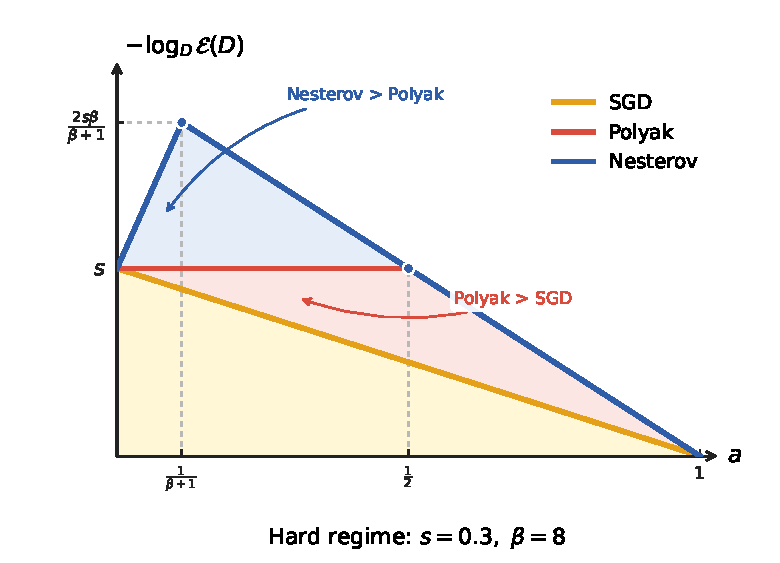
\includegraphics[
              width=\linewidth
          ]{figures/noiseless_fixed_batch_hard.pdf}
          \caption{Hard regime.}
          \label{fig:noiseless-fixed-batch-hard}
      \end{subfigure}
      \hfill
      \begin{subfigure}[t]{0.49\textwidth}
          \centering
          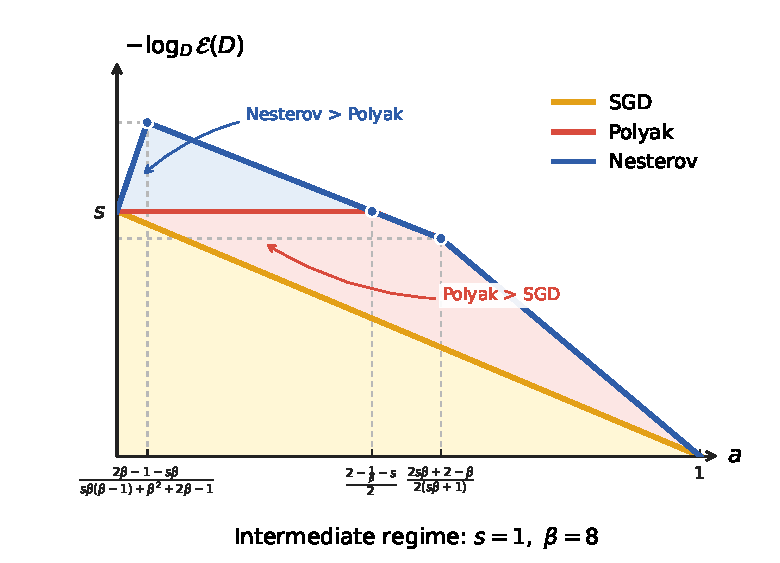
\includegraphics[
              width=\linewidth
          ]{figures/noiseless_fixed_batch_intermediate.pdf}
          \caption{Intermediate regime.}
          \label{fig:noiseless-fixed-batch-intermediate}
      \end{subfigure}

      \medskip

      \begin{subfigure}[t]{0.49\textwidth}
          \centering
          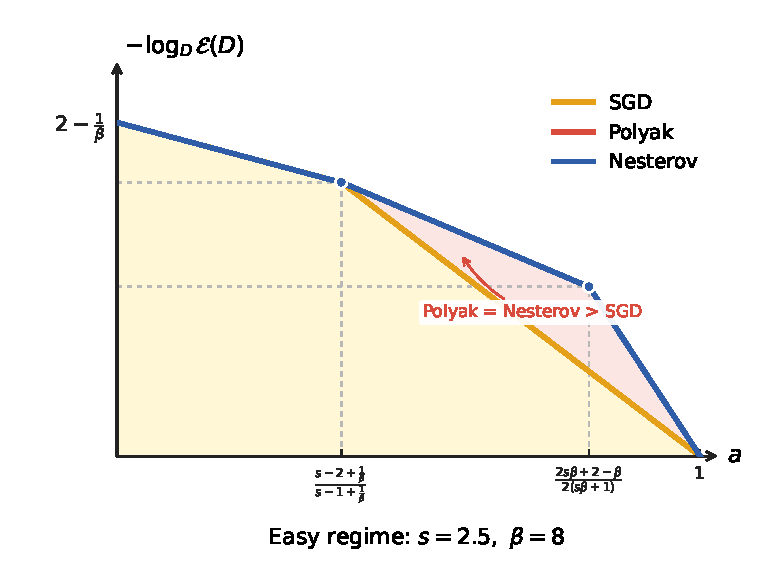
\includegraphics[
              width=\linewidth
          ]{figures/noiseless_fixed_batch_easy.pdf}
          \caption{Easy regime.}
          \label{fig:noiseless-fixed-batch-easy}
      \end{subfigure}

      \caption{
          Optimal fixed-batch data scaling rates in the noiseless setting
          for $\beta=8$. Panels (a), (b), and (c) correspond to
          Theorems~\ref{thm:fixed-batch-data-scaling-noiseless-hard},
          \ref{thm:fixed-batch-data-scaling-noiseless-intermediate}, and
          \ref{thm:fixed-batch-data-scaling-noiseless-easy}, and use
          $s=0.3$, $s=1$, and $s=2.5$, respectively. The horizontal axis
          is the batch-size exponent $a$ in $B\eqsim D^a$, and the vertical
          axis is the optimal loss-decay exponent. Yellow, red, and blue
          denote the rates attainable by SGD, Polyak momentum, and Nesterov
          momentum, respectively.
      }
      \label{fig:noiseless-fixed-batch-phase-diagrams}
  \end{figure*}
  
\begin{theorem}[Fixed-batch scaling in the easy noiseless regime]
\label{thm:fixed-batch-data-scaling-noiseless-easy}
Suppose
\(s\geq2-\frac1\beta.\)
Then
\[
r_{\mathrm{SGD}}(a)
=
\begin{cases}
\left(2-\dfrac1\beta\right)-\left(1-\dfrac1\beta\right)a,
&0\leq a\leq\dfrac{s-2+\frac1\beta}{s-1+\frac1\beta},\\[3mm]
s(1-a),
&\dfrac{s-2+\frac1\beta}{s-1+\frac1\beta}<a<1,
\end{cases}
\]
and Polyak and Nesterov momentum have the same optimal decay exponent,
\[
r_{\mathrm{Pol}}(a)
=
r_{\mathrm{Nes}}(a)
=
\begin{cases}
\left(2-\dfrac1\beta\right)-\left(1-\dfrac1\beta\right)a,
&0\leq a\leq\dfrac{s-2+\frac1\beta}{s-1+\frac1\beta},\\[3mm]
\dfrac{s\beta(3-2a)}{s\beta+\beta+1},
&\dfrac{s-2+\frac1\beta}{s-1+\frac1\beta}<a
\leq\dfrac{2s\beta+2-\beta}{2(s\beta+1)},\\[3mm]
2s(1-a),
&\dfrac{2s\beta+2-\beta}{2(s\beta+1)}<a<1.
\end{cases}
\]
At the boundaries involving the strict transient condition, the stated value is understood in the supremal sense represented by the \(o(1)\) term.
\end{theorem}

\begin{proof}
\medskip

\noindent\textbf{SGD.}
The optimal choice is \(c=0\), so the signal and multiplicative-noise powers are
\[
s(1-a)
\qquad\text{and}\qquad
\left(2-\frac1\beta\right)-\left(1-\frac1\beta\right)a.
\]
They coincide when
\(a=\frac{s-2+\frac1\beta}{s-1+\frac1\beta}.\)
The multiplicative-noise power is smaller below this point and the signal power is smaller above it, giving the stated SGD formula.

\medskip

\noindent\textbf{Polyak momentum.}
The optimum has \(c=0\), \(0\leq b\leq a\), and \(b<1-a\). At \(b=0\), the multiplicative-noise power is smaller precisely when
\(a\leq\frac{s-2+\frac1\beta}{s-1+\frac1\beta},\)
which gives the first branch. Beyond this point, increasing \(b\) balances the signal and multiplicative-noise powers, giving
\(\frac{s\beta(3-2a)}{s\beta+\beta+1}.\)
The balance reaches the transient boundary \(b=1-a\) when
\[
a=\frac{2s\beta+2-\beta}{2(s\beta+1)}.
\]
For larger \(a\), the signal power at \(b\uparrow1-a\) is smaller and equals \(2s(1-a)\).

\medskip

\noindent\textbf{Nesterov momentum.}
The optimum has \(c=0\), \(0\leq b\leq\beta a\), and \(b<1-a\). In the easy regime, the optimum either occurs at \(b=0\), at the interior balance, or at the transient boundary. Each of these choices is admissible for both Polyak and Nesterov momentum, and the Nesterov stability boundary \(b=\beta a\) is never active. Consequently Nesterov has exactly the same three branches as Polyak momentum. The adjacent expressions agree at both boundaries, completing the proof.
\end{proof}

Figure~\ref{fig:noiseless-fixed-batch-phase-diagrams} summarizes the three fixed-batch phase diagrams in Theorems~\ref{thm:fixed-batch-data-scaling-noiseless-hard}, \ref{thm:fixed-batch-data-scaling-noiseless-intermediate}, and \ref{thm:fixed-batch-data-scaling-noiseless-easy}.


\newpage
\section{Experimental Details}
\label{app:experiment}

\subsection{Stability-Boundary Experiments}
\label{app:stability-experiment}

We simulate the power-law regression model from Section~\ref{sec:plkr} in a
finite-dimensional eigenbasis. At every iteration, a fresh Gaussian
mini-batch is sampled and the corresponding stochastic-gradient update is
applied. The three algorithms are initialized from the same point, with
\(\btheta_{-1}=\btheta_0=0\). For the momentum methods, we fix
\(1-\rho=2^{-24}\), while SGD uses \(\rho=0\). We scan batch sizes
\(B\in\{2^0,2^1,\ldots,2^{12}\}\) and 50 logarithmically spaced learning
rates between \(2^{-10}\) and \(8\). Each run lasts \(K=2000\) iterations, and
the exact population excess risk is evaluated after every update.

We classify a run as stable if the average population excess risk over the
last 20 iterations is finite and smaller than \(1\). If the loss becomes
non-finite or exceeds \(10^{12}\) during training, the run is terminated and
classified as unstable. For each algorithm, batch size, and random seed, the
empirical stability boundary is the largest learning rate on the search grid
that passes this criterion. We repeat the search over five independent random
seeds. The markers in Figure~\ref{fig:stability-beta15} report the
arithmetic mean of the five per-seed stability boundaries.

The dashed lines are fitted only after the empirical boundaries have been
computed. For Polyak momentum, we fix the slope to the theoretical form
\(B(1-\rho)\) and fit its multiplicative constant using all finite boundary
points. For Nesterov momentum, we divide the points at the onset of the visible
large-batch plateau. The points before this split are fitted to
\(B^\beta(1-\rho)\), with the exponent fixed to its theoretical value, whereas
the points after the split are fitted by a constant horizontal level. In each
case, the multiplicative constant or horizontal level is the geometric mean
of the pointwise ratios in log scale. The dotted vertical line indicates this
split; it affects only the reference fits and not the empirical stability
classification.

Figure \ref{fig:additional-stability-boundaries} presents additional empirical stability-boundary results under different choices of the source exponent \(s\) and capacity exponent \(\beta\).

\subsection{Data Scaling Experiments}
\label{app:data-scaling-experiments}
We simulate the power-law regression model with \(d=4096\), \(s=0.3\), \(\beta=4\), \(\sigma=0.1\), and \(D\in\{2000,4000,8000,16000,32000,64000,128000\}\). All algorithms are initialized at \(\btheta_{-1}=\btheta_0=\bm0\). At each iteration, we independently sample Gaussian noise according to the curvature-aligned covariance model in Proposition~\ref{prop:noise-geometry}.

\begin{figure*}
    \centering
    \begin{subfigure}[t]{0.325\textwidth}
        \centering
        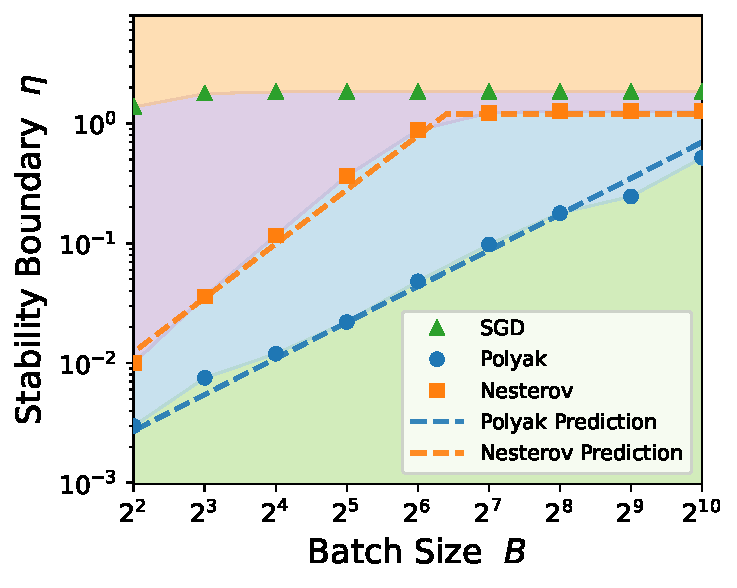
\includegraphics[width=\linewidth]{figures/beta1_5s3_plot.pdf}
        \caption{\(s=0.3,\beta=1.5\)}
    \end{subfigure}
    \hfill
    \begin{subfigure}[t]{0.325\textwidth}
        \centering
        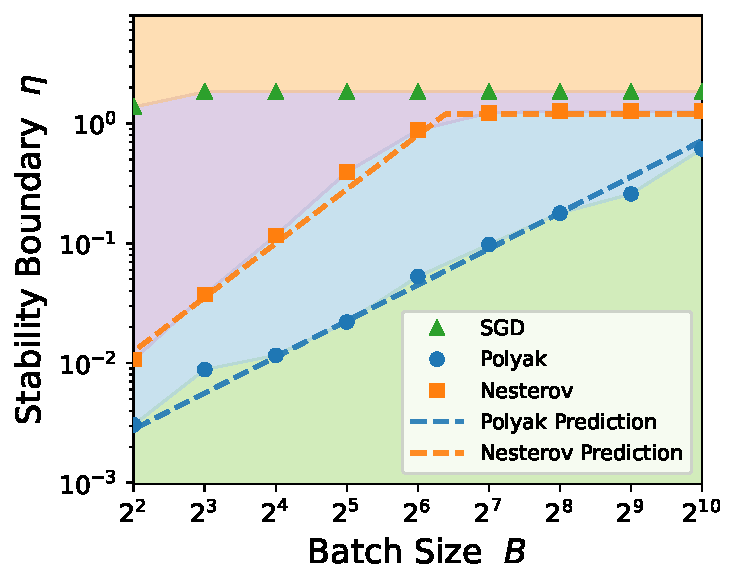
\includegraphics[width=\linewidth]{figures/beta1_5s5_plot.pdf}
        \caption{\(s=0.5,\beta=1.5\)}
    \end{subfigure}
    \hfill
    \begin{subfigure}[t]{0.325\textwidth}
        \centering
        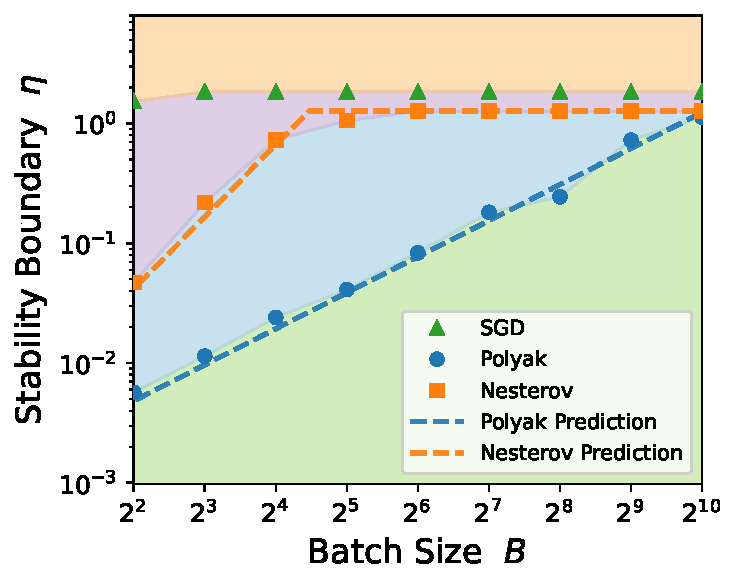
\includegraphics[width=\linewidth]{figures/beta2s2_plot.pdf}
        \caption{\(s=0.2,\beta=2\)}
    \end{subfigure}
    \medskip
    \begin{subfigure}[t]{0.325\textwidth}
        \centering
        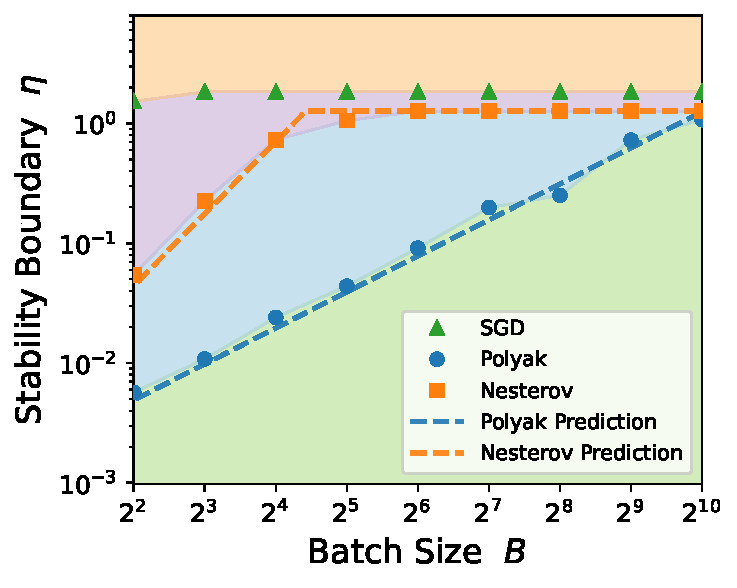
\includegraphics[width=\linewidth]{figures/beta2s3_plot.pdf}
        \caption{\(s=0.3,\beta=2\)}
    \end{subfigure}
    \hfill
    \begin{subfigure}[t]{0.325\textwidth}
        \centering
        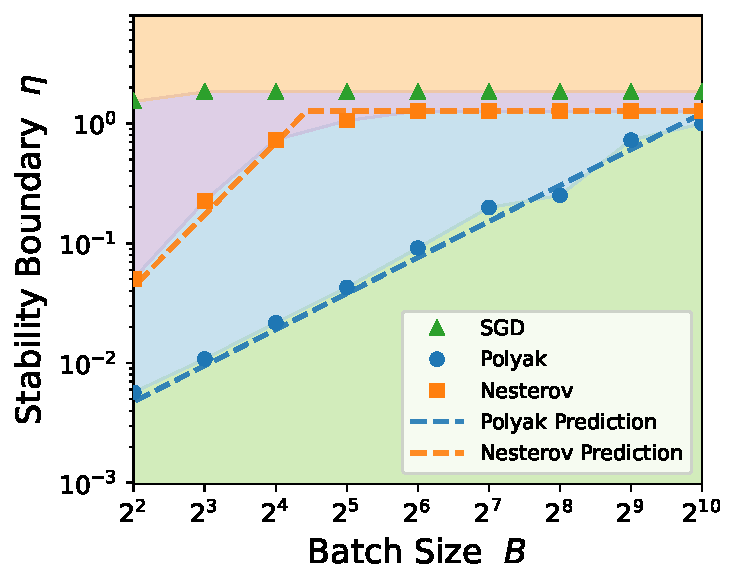
\includegraphics[width=\linewidth]{figures/beta2s5_plot.pdf}
        \caption{\(s=0.5,\beta=2\)}
    \end{subfigure}
    \hfill
    \begin{subfigure}[t]{0.325\textwidth}
        \centering
        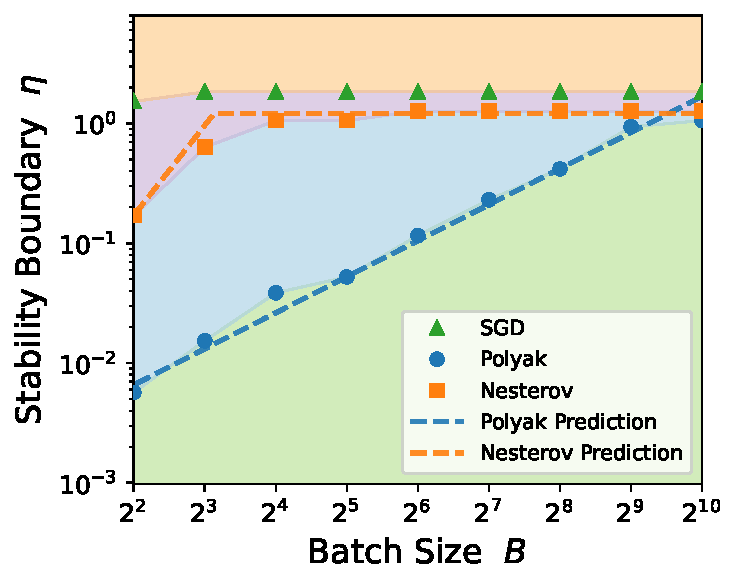
\includegraphics[width=\linewidth]{figures/beta2_5s3_plot.pdf}
        \caption{\(s=0.3,\beta=2.5\)}
    \end{subfigure}
    \medskip
    \begin{subfigure}[t]{0.32\textwidth}
        \centering
        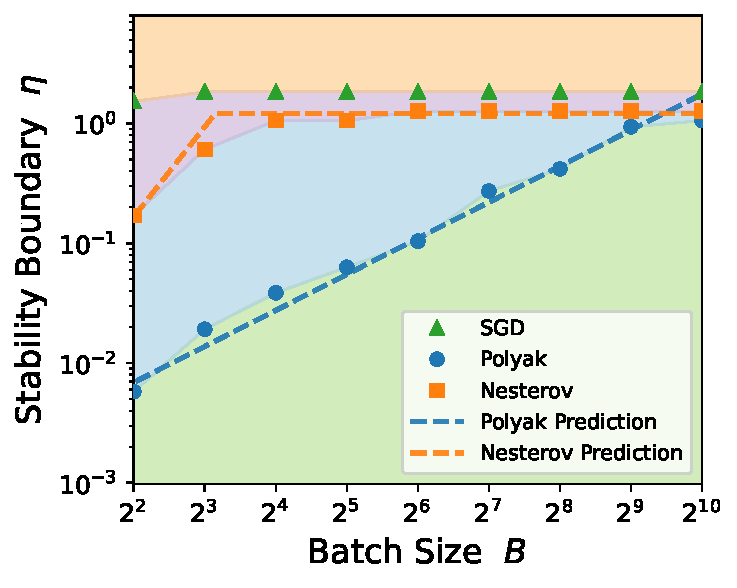
\includegraphics[width=\linewidth]{figures/beta2_5s5_plot.pdf}
        \caption{\(s=0.5,\beta=2.5\)}
    \end{subfigure}
    \caption{Additional empirical stability boundaries under different choices of \(s\) and \(\beta\)}
    \label{fig:additional-stability-boundaries}
\end{figure*}

\paragraph{Polyak critical-batch experiment.}
We compare SGD and Polyak momentum at \(B\eqsim D^{\frac{s}{s+1}}\) and \(B\eqsim D^{\frac{2s}{s+1}}\), with \(K=\lfloor D/B\rfloor\). At the smaller batch size, SGD uses \(\eta=0.1\), while Polyak uses \(\eta=0.1D^{-\frac{s}{s+1}}\) and \(1-\rho=D^{-\frac{s}{s+1}}\). At the larger batch size, SGD uses \(\eta=0.5\), while Polyak uses \(\eta=0.1\) and \(1-\rho=D^{-\frac{s}{s+1}}\). Each point reports the mean final excess risk over \(100\) independent runs.

\paragraph{Nesterov large-batch experiment.}
All three algorithms use \(B=\operatorname{round}(0.15D^a)\) and \(K=\lfloor D/B\rfloor\), where
\[
a=\frac{2s\beta+1}{2s\beta+\beta+1}-0.05.
\]
SGD uses \(\eta=0.3\). Polyak uses \(\eta=0.1\) and \(1-\rho=D^{-(a-\frac{s}{s+1})}\). For Nesterov, defining \(x=\frac{s\beta-(\beta-1)a}{s\beta+1}\), we use \(\eta=0.1\) and \(1-\rho=2D^{-(a-x)}\). Each point reports the mean over \(100\) independent runs of the excess risk averaged over the final \(1\%\) of training. 
